\documentclass[11pt]{book}

% Users of the {thebibliography} environment or BibTeX should use the
% scicite.sty package, downloadable from *Science* at
% www.sciencemag.org/about/authors/prep/TeX_help/ .
% This package should properly format in-text
% reference calls and reference-list numbers.

%\usepackage{scicite}

% Use times if you have the font installed; otherwise, comment out the
% following line.

%\usepackage{times}
\usepackage{apacite}
\usepackage{amsmath}
\usepackage{amsfonts} 
%\usepackage{algorithmic}
%\usepackage{algpseudocode}

% The preamble here sets up a lot of new/revised commands and
% environments.  It's annoying, but please do *not* try to strip these
% out into a separate .sty file (which could lead to the loss of some
% information when we convert the file to other formats).  Instead, keep
% them in the preamble of your main LaTeX source file.


% The following parameters seem to provide a reasonable page setup.

\usepackage[margin=1.3in]{geometry}
\usepackage{xcolor}
\usepackage{color}
%\usepackage{tabularx}



\usepackage[T1]{fontenc}
\usepackage[utf8]{inputenc}

\usepackage{algorithm}
\usepackage{algpseudocode}
\usepackage{chngcntr}
\usepackage{dirtytalk}
\usepackage{dsfont}
\usepackage[shortcuts]{extdash}
\usepackage{fancyhdr}
\usepackage{float}
\usepackage{hyphenat}
\usepackage{mathtools}
\usepackage{moresize}
\usepackage{newunicodechar}
\usepackage{nicefrac}
\usepackage{setspace}
%\usepackage{subcaption}
%\usepackage{algorithm2e}
\usepackage{titlesec}
\usepackage{xr}
\usepackage{xspace}

\usepackage{amsmath}
\usepackage{amssymb}
\usepackage{amscd}
\usepackage{mathtools}

\makeatletter\@ifclassloaded{ieeeconf}{}{
	\usepackage{amsmath, amssymb, amscd}
}\makeatother

\usepackage{cleveref}\newcommand*{\crefrangeconjunction}{--}
\usepackage[nonumberlist, nopostdot, sort=def]{glossaries}\glsdisablehyper\makenoidxglossaries
\usepackage{mathabx}
\usepackage{mleftright}
\usepackage{pdfpages}
\usepackage{thmtools}
\usepackage{zref}

%consecutive equation numbering across chapters
\makeatletter
\ifcsname c@chapter\endcsname
\counterwithout{equation}{chapter}
\fi
\makeatother
\newcommand*\num{\addtocounter{equation}{1}\tag{\theequation}}

\newtheorem{thm}{Theorem}
\newtheorem{defn}{Definition}
\newtheorem{lem}{Lemma}
\newtheorem{prob}{Problem}


\newcommand*{\elab}[1]{\label{eq:#1}}
\newcommand*{\eref}[1]{\eqref{eq:#1}}
\newcommand*{\slab}[1]{\label{sec:#1}}
\newcommand*{\sref}[1]{Section~\ref{sec:#1}}

\newcommand*{\B}[1]{\mathbf{#1}}
\newcommand*{\C}[1]{\mathcal{#1}}
\newcommand*{\F}[1]{\mathbb{#1}}
\newcommand*{\R}[1]{\mathrm{#1}}
\newcommand*{\M}[1]{\strut\smash{#1}}
\newcommand*{\V}[1]{\texttt{#1}}
\newcommand*{\Z}[1]{\mathds{#1}}

\DeclareMathOperator{\1}{\Z1}
\DeclareMathOperator*{\argmax}{arg\,max}
\DeclareMathOperator*{\argmin}{arg\,min}
\let\S\undefined\DeclareMathOperator{\S}{\Sigma}
\DeclareMathOperator{\cov}{cov}
\DeclareMathOperator{\D}{\Z D}
\DeclareMathOperator{\diag}{diag}
\DeclareMathOperator{\dif}{\partial}
\DeclareMathOperator{\Do}{do}
\DeclareMathOperator{\E}{\Z E}
\DeclareMathOperator{\erf}{erf}
\DeclareMathOperator{\EVD}{EVD}
\let\H\undefined\DeclareMathOperator{\H}{\Z H}
\DeclareMathOperator{\I}{\Z I}
\DeclareMathOperator{\p}{\Z P}
\DeclareMathOperator{\rank}{rank}
\DeclareMathOperator{\range}{range}
\DeclareMathOperator*{\softmin}{soft\,min}
\DeclareMathOperator{\spn}{span}
\DeclareMathOperator{\tr}{tr}

\newcommand*{\+}{\dag}
\newcommand*{\ccell}[1]{\omit\hfil$\displaystyle#1$\hfil}
\newcommand*{\const}{\textnormal{const}}
\newcommand*{\copr}{\pagestyle{fancy}\thispagestyle{fancy}\renewcommand{\headrulewidth}{0pt}\lhead{}\rhead{}\rfoot{\tiny Roy Fox, \the\year}}
\newcommand*{\dash}{\mathrel{\textnormal{ --- }}}
\newcommand*{\defeq}{\stackrel{\mathclap{\text{def}}}{=}}
\newcommand*{\dto}{\twoheadrightarrow}
\newcommand*{\eq}[1]{\begin{align*}#1\end{align*}}
\newcommand*{\eqa}[1]{\begin{aligned}#1\end{aligned}}
\newcommand*{\eqat}[2]{\begin{alignat*}{#1}#2\end{alignat*}}
\newcommand*{\eqatn}[2]{\begin{alignat}{#1}#2\end{alignat}}
\newcommand*{\eqdat}[2]{\begin{alignedat}{#1}#2\end{alignedat}}
\newcommand*{\eqg}[1]{\begin{gather*}#1\end{gather*}}
\newcommand*{\eqn}[1]{\begin{align}#1\end{align}}
\newcommand*{\eqs}[1]{\begin{subequations}#1\end{subequations}}
\newcommand*{\figinc}[3]{\begin{figure}\centering\includegraphics[#1]{#2}\caption{#3}\label{fig:#2}\end{figure}}
\newcommand*{\figinp}[2]{\begin{figure}\centering\vspace{.5em}\input{#1}\vspace{-.5em}\caption{#2}\label{fig:#1}\end{figure}}
\newcommand*{\getsto}{\leftrightarrow}
\newcommand*{\given}{\vert}
\newcommand*{\idag}{{\rotatebox[origin=c]{180}{$\scriptstyle\dag$}}}
\newcommand*{\lan}{\langle}
\newcommand*{\lr}[1]{\mleft(#1\mright)}
\newcommand*{\lra}[1]{\mleft\lan#1\mright\ran}
\newcommand*{\lrc}[1]{\mleft\{#1\mright\}}
\newcommand*{\lrs}[1]{\mleft[#1\mright]}
\newcommand*{\mat}[1]{\begin{bmatrix}#1\end{bmatrix}}
\newcommand*{\matr}[1]{\begin{bmatrix*}[r]#1\end{bmatrix*}}
\newcommand*{\mrlap}{\mathrlap}
\newcommand*{\nd}{\prec}
\newcommand*{\nsd}{\preceq}
\newcommand*{\nn}{\nonumber}
\newcommand*{\opt}[3]{\eqat{2}{&\ccell{#1}&\quad&#2\\&\ccell{\st}&&#3}}
\newcommand*{\optn}[3]{\eqatn{2}{&\ccell{#1}&\quad&#2\\&\ccell{\st}&&#3}}
\newcommand*{\pd}{\succ}
\newcommand*{\pro}{\mathrel{\propto}}
\newcommand*{\psd}{\succeq}
\newcommand*{\ran}{\rangle}
\newcommand*{\st}{\textnormal{s.t.}}
\newcommand*{\subs}{\subseteq}
\newcommand*{\T}{\intercal}
\newcommand*{\TODO}[1]{\footnote{#1}}
\renewcommand*{\vdots}{\vbox{\baselineskip=4pt\lineskiplimit=0pt\kern2pt\hbox{.}\hbox{.}\hbox{.}}}
\newcommand*{\x}{\times}
\newcommand*{\xto}[1][]{\xrightarrow[#1]{}}



\newcommand{\detectlib}{\texttt{IsoDetect}\xspace}
\newcommand{\company}{\texttt{Company X}\xspace}
\newcommand{\cond}{\textrm{pred}\xspace}
\newcommand{\dataset}{data set\xspace}
\newcommand{\datasets}{data sets\xspace}
\newcommand{\spview}{\textsf{SPView}\xspace}
\newcommand{\fjview}{\textsf{FJView}\xspace}
\newcommand{\aggview}{\textsf{AggView}\xspace}
\newcommand{\hashfunc}[1]{\textsf{hash}(#1)\xspace}
\newcommand{\hashop}{\textsf{hash}\xspace}
\newcommand{\nsc}{\textsf{NormalizedSC}\xspace}
\newcommand{\rsc}{\textsf{RawSC}\xspace}

\newcommand{\avgfunc}{\ensuremath{\texttt{avg} }\xspace}
\newcommand{\maxfunc}{\ensuremath{\texttt{max} }\xspace}
\newcommand{\minfunc}{\ensuremath{\texttt{min} }\xspace}
\newcommand{\histfunc}{\ensuremath{\texttt{histogram\_numeric} }\xspace}
\newcommand{\countfunc}{\ensuremath{\texttt{count}}\xspace}
\newcommand{\sumfunc}{\ensuremath{\texttt{sum} }\xspace}
\newcommand{\varfunc}{\ensuremath{\texttt{var} }\xspace}
\newcommand{\stdfunc}{\ensuremath{\texttt{std} }\xspace}
\newcommand{\covfunc}{\ensuremath{\texttt{cov} }\xspace}
\newcommand{\corrfunc}{\ensuremath{\texttt{corr} }\xspace}
\newcommand{\medfunc}{\ensuremath{\texttt{median} }\xspace}
\newcommand{\percfunc}{\ensuremath{\texttt{percentile} }\xspace}
\newcommand{\havingfunc}{\ensuremath{\texttt{HAVING} }\xspace}
\newcommand{\selectfunc}{\ensuremath{\texttt{select} }\xspace}
\newcommand{\ratio}{\ensuremath{\rho }\xspace}


\newcommand{\insertion}{\ensuremath{\texttt{INSERT} }\xspace}
\newcommand{\update}{\ensuremath{\texttt{UPDATE} }\xspace}
\newcommand{\delete}{\ensuremath{\texttt{DELETE} }\xspace}

\newcommand{\sysfull}{AlphaClean\xspace}
\newcommand{\sys}{AlphaClean\xspace}
\newcommand{\sysnospace}{AlphaClean}
\newcommand{\alg}{DDO\xspace}
\newcommand{\tsc}{TSC\xspace}


\newcommand{\tbl}[1]{\textsf{#1}\xspace}
\newcommand{\field}[1]{\textsf{#1}\xspace}
\newcommand{\cost}{\textrm{cost}\xspace}
\newcommand{\ans}{\textsf{ans}\xspace}
\newcommand{\dans}{\Delta\textsf{ans}\xspace}
\newcommand{\cqp}{correction query processing\xspace}
\newcommand{\Cqp}{Correction query processing\xspace}

\newcommand{\reminder}[1]{{{\textcolor{magenta}{\{\{\bf #1\}\}}}\xspace}}
\newcommand{\ewu}[1]{{{\textcolor{blue}{\{\{\bf ewu:\} #1\}}}\xspace}}
\newcommand{\mps}[1]{{{\textcolor{red}{\{\{\bf meelap:\} #1\}}}\xspace}}
\newcommand{\stitle}[1]{\smallskip\noindent\textbf{#1: }}
\newcommand{\ititle}[1]{\smallskip\noindent\textit{#1: }}
\newcommand{\btitle}[1]{\smallskip\noindent\textbf{#1}}


\definecolor{light-gray}{gray}{0.95}
\definecolor{mid-gray}{gray}{0.85}
\definecolor{green}{RGB}{0,176,80}
\definecolor{darkred}{rgb}{0.7,0.25,0.25}
\definecolor{darkgreen}{rgb}{0.15,0.55,0.15}
\definecolor{darkblue}{rgb}{0.1,0.1,0.5}
\definecolor{orange}{RGB}{237,125,49}
\definecolor{blue}{RGB}{68,114,196}
\definecolor{pop}{RGB}{0,21,245}

\newcommand{\white}[1]{{\textcolor{white}{#1}\xspace}}
\newcommand{\blue}[1]{{\textcolor{blue}{{\bf #1}}\xspace}}
\newcommand{\orange}[1]{{\textcolor{orange}{{\bf #1}}\xspace}}
\newcommand{\pop}[1]{{\textcolor{pop}{{\textit{\textbf{#1}}}}\xspace}}
\newcommand{\red}[1]{\textcolor{red}{#1}}
\newcommand{\green}[1]{\textcolor{green}{#1}}
\newcommand{\gray}[1]{\textcolor{light-gray}{#1}}




\newcommand{\specialcell}[2][c]{%
  \begin{tabular}[#1]{@{}c@{}}#2\end{tabular}}

\def\ojoin{\setbox0=\hbox{$\bowtie$}%
  \rule[-.02ex]{.25em}{.4pt}\llap{\rule[\ht0]{.25em}{.4pt}}}
\def\leftouterjoin{\mathbin{\ojoin\mkern-5.8mu\bowtie}}
\def\rightouterjoin{\mathbin{\bowtie\mkern-5.8mu\ojoin}}
\def\fullouterjoin{\mathbin{\ojoin\mkern-5.8mu\bowtie\mkern-5.8mu\ojoin}}
%%\IEEEoverridecommandlockouts
%\overrideIEEEmargins

%floats and figures
%\usepackage{graphics} %imported in the main document.
%\usepackage[pdftex]{graphicx}
\usepackage[font={small}]{caption}
\usepackage{subcaption}
%\usepackage[center]{subfigure} %DONT USE BOTH SUBCAPTION AND SUBFIGURE
%\DeclareGraphicsExtensions{.pdf,.png,.jpg}
%\usepackage{overpic}
\usepackage[rightcaption]{sidecap}
%\usepackage{pbox}

%Math Stuff
\

%DOCUMENT WIDE
\usepackage{times} % assumes new font selection scheme installed
\usepackage{xspace}
%\usepackage[english]{babel} %for hyphenation rules
%\usepackage{flushend}%balance columns on last page
\usepackage{fixltx2e} %fix latex issue across versions
\usepackage{bm}
\usepackage{units}
\usepackage{subfiles} %individual file compilation--makes it quick 
\usepackage{setspace}%line spacing within document

\usepackage{makeidx}
\usepackage{enumitem}
\usepackage[yyyymmdd,hhmmss]{datetime}
\usepackage[english]{babel}

%Bibliography and cross-ref
\makeatletter
\let\NAT@parse\undefined
\makeatother
\usepackage[numbers]{natbib}
\renewcommand{\bibfont}{\footnotesize}
% \usepackage{cite} %DONT USE NATBIB AND CITE TOGETHER

%hyperlinking
\usepackage{url}
\makeatletter
\g@addto@macro{\UrlBreaks}{\UrlOrds}
\makeatother
\usepackage{color}
%\usepackage[usenames,dvipsnames,table,xcdraw]{xcolor}
\usepackage[T1]{fontenc}


%=======U S E R  D E F I N E D  M A C R O S=======
% \newcommand{\bibhref}[2]{#2}
\newcommand{\todo}[1]{\textcolor{red}{[?#1?]}}
\newcommand{\tocite}[1]{\textcolor{red}{[cite]}}
\newcommand{\del}[1]{}
\newcommand{\etal}[1]{et al.}

% Usage:
% \figlabel{myfigure} creates \label{fig:myfigure}
% \figref{myfigure} references it
\newcommand{\figlabel}[1]{\label{fig:#1}}
\newcommand{\figref}[1]{Figure~\ref{fig:#1}}

% Usage:
% \seclabel{mysection} creates \label{sec:mysection}
% \secref{mysection} references it
\newcommand{\seclabel}[1]{\label{sec:#1}}
\newcommand{\secref}[1]{Section~\ref{sec:#1}}

% Usage:
% \tablabel{mytable} creates \label{tab:mytable}
% \tabref{mytable} references it
\newcommand{\tablabel}[1]{\label{tab:#1}}
\newcommand{\tabref}[1]{Table~\ref{tab:#1}}

% use this command instead of writing "da Vinci" so it's never split 
\newcommand{\davinci}{da~Vinci\xspace}

%for table
% \usepackage{floatrow}
% Table float box with bottom caption, box width adjusted to content
% \newfloatcommand{capbtabbox}{table}[][\FBwidth]

%The next command sets up an environment for the abstract to your paper.

\newenvironment{sciabstract}{%
\begin{quote} \bf}
{\end{quote}}
\newcommand{\hirl}{SWIRL\xspace}
\newcommand{\tpsalgo}{TPS\xspace}
\newcommand{\HIRL}{SWIRL\xspace}

% If your reference list includes text notes as well as references,
% include the following line; otherwise, comment it out.

\renewcommand\refname{References and Notes}

% The following lines set up an environment for the last note in the
% reference list, which commonly includes acknowledgments of funding,
% help, etc.  It's intended for users of BibTeX or the {thebibliography}
% environment.  Users who are hand-coding their references at the end
% using a list environment such as {enumerate} can simply add another
% item at the end, and it will be numbered automatically.

\newcounter{lastnote}
\newenvironment{scilastnote}{%
\setcounter{lastnote}{\value{enumiv}}%
\addtocounter{lastnote}{+1}%
\begin{list}%
{\arabic{lastnote}.}
{\setlength{\leftmargin}{.22in}}
{\setlength{\labelsep}{.5em}}}
{\end{list}}

\newtheorem{theorem}{Theorem}
\newtheorem{example}{Example}
\newtheorem{definition}{Definition}
\newtheorem{problem}{Problem}
\newtheorem{property}{Property}
\newtheorem{proposition}{Proposition}
\newtheorem{lemma}{Lemma}
\newtheorem{corollary}{Corollary}


% Include your paper's title here

\title{Policy Search in Markov Decision Processes with High Dimensional Action Spaces and Long Time Horizons} 

% Place the author information here.  Please hand-code the contact
% information and notecalls; do *not* use \footnote commands.  Let the
% author contact information appear immediately below the author names
% as shown.  We would also prefer that you don't change the type-size
% settings shown here.

\author
{Sanjay Krishnan\\
\\
\normalsize{$^{1}$Department of Electrical Engineering and Computer Science, University of California Berkeley,}\\
\normalsize{$^\ast$To whom correspondence should be addressed; E-mail:  sanjay@eecs.berkeley.edu.}
}

% Include the date command, but leave its argument blank.

\date{}



%%%%%%%%%%%%%%%%% END OF PREAMBLE %%%%%%%%%%%%%%%%



\begin{document} 

% Double-space the manuscript.

\baselineskip26pt

% Make the title.

\maketitle 



% Place your abstract within the special {sciabstract} environment.


\begin{sciabstract}
Markov Decision Processes are ubiquitous from problems in robot path planning to cluster task scheduling. 
Policy search in MDPs suffers greatly from the ``curse of dimensionality'' when the space of possible decisions at each time-step is very high-dimensional or when time horizon is very long. 
This main thesis of this dissertation is that it is possible to learn important structural features of an MDP to guid the search process from offline data to significantly improve the sample-efficiency, stability, and robustness of solutions even with high dimensional action spaces and long time horizons.
It presents applications to surgical robot control, data cleaning, and generating efficient execution plans for relational queries. 
The dissertation contributes: (1) Sequential Windowed Reinforcement Learning: a framework that approximates a long-horizon MDP with a sequence of shorter term MDPs with smooth quadratic cost functions from a small number of expert demonstrations, (2) Deep Discovery of Options: an algorithm that discovers hierarchical structure in the action space from observed demonstrations, (3) AlphaClean: a system that decomposes a data cleaning task into a set of independent search problems and uses deep q-learning to share structure across the problems, and (4) Learning Query Optimizer: a system that observes executions of a dynamic program for SQL query optimization and learns a model to predict cost-to-go values to greatly speed up future search problems. 
\end{sciabstract}


\clearpage

\tableofcontents

\clearpage


% In setting up this template for *Science* papers, we've used both
% the \section* command and the \paragraph* command for topical
% divisions.  Which you use will of course depend on the type of paper
% you're writing.  Review Articles tend to have displayed headings, for
% which \section* is more appropriate; Research Articles, when they have
% formal topical divisions at all, tend to signal them with bold text
% that runs into the paragraph, for which \paragraph* is the right
% choice.  Either way, use the asterisk (*) modifier, as shown, to
% suppress numbering.



\setcounter{secnumdepth}{0}
\chapter{Introduction}
Bellman's ``Principle of Optimality'' and the characterization of dynamic programming is one of the most important results in computing~\cite{bellman2013dynamic}. Its importance stems from the ubiquity of Markovian decision processes (MDPs), which formalize a wide range of problems from path planning to scheduling~\cite{howard1966dynamic}. In the most abstract form, there is an agent who makes a sequence of decisions to effect change on a system that processes these decisions and updates its internal state possibly non-deterministically. 
The process is ``Markovian'' in the sense that the system's current state completely determines its future progression. As an example of an MDP, one might have to plan a sequence of motor commands to a robot to control it to a target position. Or, one might have to schedule a sequence of cluster computing tasks while avoiding double scheduling on a node. 
The solution to a MDP is a decision making policy: the optimal decision to make given any current state of the system. 

Since the MDP framework is extremely general---it encompasses shortest-path graph search, supervised machine learning, and optimal control---the difficulty in solving a particular MDP relates to what assumptions can be made about the system.
A setting of interest is when one only assumes black-box access to the system, where no parametric model of the system is readily available and the agent must iteratively query the system to optimize its decision policy.
This setting, also called \emph{reinforcement learning}~\cite{sutton1998reinforcement}, has been the subject of significant recent research interest.
First, there are many dynamical problems for which a closed-form analytical description of a system's behavior is not available but one has a programatic approximation of how the system transitions (i.e., simulation).
Reinforcement Learning (RL) allows for direct optimization of decision policies over such simulated systems.
Next, by virtue of the minimal assumptions, RL algorithms are extremely general and widely applicable across many different problem settings.
From a software engineering perspective, this unification allows the research community to develop a small number of optimized libraries for RL rather each domain designing/maintaining problem-specific algorithms.
Over the last few years, the combination deep neural networks and reinforcement learning, or Deep RL, have emerged as in robotics, AI, and machine learning as an important area of research~\cite{mnih2015human,silver2017mastering, sunderhauf2018limits, stoica2017berkeley}.
Deep RL correlates features of states to successful decisions using neural networks. 

Due to the nature of these black-box queries, RL can be very inefficient in problems where the decision space is high-dimensional and when the decision horizon (the length of the sequence of decisions the agent needs to make) is very long. 
The algorithm has to simultaneously correlate features that are valuable for making a decision in a state while also searching through the space of decisions to figure out which sequence of decisions are valuable. A failure to learn means that the algorithm cannot intelligently search the space of decisions, and a failure to find promising sequences early means that the algorithm cannot learn.
This creates a fundementally unstable algorithm setting, where the hope is the algorithm discovers good decision sequences by chance and can bootstrap from these relatively rare examples.
The higher the dimensionality of the problem, the less likely purely random search will be successful. 

Since Deep RL suffers such limitations, how do practioners solve such large scale ``black-box'' problems today (with non-Deep RL methods)? Every domain has pragmatic approximation algorithms that exploit heuristics, domain knowledge, and other known structure of typical solutions in the problem domain. Consider the following examples:

\begin{example}[SQL Query Optimization]
Most relational database management systems support only dyadic join operations (joining two tables) as primitive operations, a query optimizer must choose the ``best'' sequence of two-way joins to achieve the k-way join of tables requested by a query. The exhaustive decision space is super exponential in k. Since it is common for data to be organized in one large table with several smaller reference tables and typical cost functions are linear in the size of the input tables, most query optimization algorithms restrict their search to left-deep plans.
\end{example}

\begin{example}[Robot Task and Motion Planning]
Planning collision free motions of a robot to meet a control objective is exponential in the time-horizon. Long-term tasks are decomposed into shorter nearly independently solvable planning subtasks. This reduces the effective planning horizon and allows the robot to reuse plans if a subtask is repeated.
\end{example}

Exploiting such structure in Deep RL poses a dilemma---either one sacrifices generality by incorporating problem-specific knowledge into the Deep RL algorithm or one pays the price of exploring an immense search space. Building and maintaining domain-specific Deep RL implementations defeats the unifying premise of Deep RL.

In several domains of interest, a limited amount of expert knowledge is available, e.g., a human teleoperator can guide the motion of a robot to show an example solution of one problem instance.
Collecting such ``demonstrations'' to exhaustively learn a solution for possible progressions on MDP can be very challenging (called imitation learning~\cite{osa2018algorithmic}), but we might have sufficient data to find important structural features of a search problem including task decomposition, subspaces of actions that are irrelevant to the task, and the structure of the cost function.
My thesis is that \emph{learning such structure can significantly improve the sample-efficiency, stability, and robustness of Deep RL in high-dimensional and long-horizon search problems.} 
With this additional supervision, the search process can be restricted to those sequences that are similar to the supervision provided by the expert.
My work over the last 6 years explores this architecture in several Deep RL systems for control of imprecise cable-driven surgical robots, automatically synthesizing data-cleaning programs to meet quality specifications, and generating efficient execution plans for relational queries. I describe algorithmic contributions, theoretical analysis about the implementations themselves, and the architecture of the RL systems.

\vspace{0.75em} \noindent \textbf{Contributions: }  This dissertation contributes:

\begin{enumerate}
    \item Deep Discovery of Options (DDO): A new bayesian learning framework for learning parametrized control hierarchies from expert data (Chapter 2). DDO infers the parameters of an Abstract HMM model to decomposes the action space into a hierarchy of discrete skills relevant to a task. I show that the hierarchical model represents policies more efficiently (requires less data to learn) than a flat model on real and simulated robot control tasks. I also show that this hierarchy can be used to guide exploration in search problems through compositions of the discrete skills seen in the data rather than arbitrary sequences of actions. I apply this model to significantly accelerate learning in self-play of Atari games.

    \emph{Krishnan, Sanjay, Roy Fox, Ion Stoica, and Ken Goldberg. DDDO: Discovery of Deep Continuous Options for Robot Learning from Demonstrations. Proceeding of Machine Learning Research: Conference on Robot Learning. 2017.} 
    
    \item Sequential Windowed Inverse Reinforcement Learning (SWIRL): A learning framework for approximating an MDP with a sequence of shorter horizon MDPs with quadratic cost functions (Chapter 3). SWIRL can be thought of as a special parametric case of DDO where skills terminate at goal states. I show on two surgical robot control tasks, cutting along a line and tensioning fabric, SWIRL significantly reduces the policy search time of a Q-Learning algorithm. I also demonstrate improvements in a robot planning task (parallel parking a car with noisy dynamics) and classical control problems (controlling a two-link pendulum).

    \emph{Krishnan, Sanjay, Animesh Garg, Richard Liaw, Brijen Thananjeyan, Lauren Miller, Florian T. Pokorny, and Ken Goldberg. SWIRL: A Sequential Windowed Inverse Reinforcement Learning Algorithm for Robot Tasks with Delayed Rewards. International Journal of Robotics Research. 2018.}

    \item Transition State Clustering (TSC): The underlying task decomposition algorithm in SWIRL is a Bayesian clustering framework called TSC (Chapter 3). This model correlates spatial and temporal features with changes in motion of the demonstrator. The crucial advantage of this framework is that it can exploit ``third person'' demonstrations data where only the states of the MDP are visible but not the decisions the expert took. The motivating application is learning from expert surgeons by analyzing data from a surgical robot. I show that TSC is more robust to spatial and temporal variation compared to other segmentation methods and can apply to both kinematic and visual demonstration data.

    \emph{Krishnan, Sanjay, Animesh Garg, Sachin Patil, Colin Lea, Gregory Hager, Pieter Abbeel, and Ken Goldberg. Transition State Clustering: Unsupervised surgical trajectory segmentation for robot learning. International Journal of Robotics Research. 2018.}

    \item Alpha Clean: A system for synthesizing data cleaning programs to enforce database integrity constraints (Chapter 4). The main algorithm in the system decomposes the integrity constraints on a table into a collection of independent search problems called blocks. The algorithm starts by exhaustively searching the initial blocks and then incrementally learns a Q-function to make the search on future increasingly precise. This process leverages the fact that data cleaning is not an arbitrary constraint satisfaction problem and most database corruption is systematic, i.e., correlated with features of the data. 

     \emph{Krishnan, Sanjay, Eugene Wu, Michael Franklin, and Ken Goldberg. Alpha Clean: Data Cleaning with Distributed Tree Search and Learning. 2018.}

    \item A new approximate dynamic programming framework for SQL query optimization. Classical query optimizers leverage dynamic programs for optimally nesting join queries. This process creates a table that memoizes cost-to-go estimates of intermediate subplans. By representing the memoization table with a neural network, the optimizer can estimate the cost-to-go of even previously unseen plans allowing for a vast expansion of the search space. I show that this process is a form of Deep Q-Learning where the state is a query graph and the actions are contractions on the query graph. One key result is that the same optimization algorithm can adaptively learn search strategies for both in-memory databases (where the search space is often heuristically restricted based to maximize index accesses) and disk-based databases (where the search space is often heuristically restricted to maximize re-use of intermediate results).

    \emph{Krishnan, Sanjay, Zongheng Yang, Ion Stoica, Joseph Hellerstein, and Ken Goldberg. Learning to Efficiently Enumerate Joins with Deep Reinforcement Learning. 2018.}
    
    \item An application of deep reinforcement learning to synthesizing surgical thin tissue tensioning policies. To improve the search time, the algorithm initializes its search with an analytical approximation of the equilibrium state of a FEM simulator. The result is a search algorithm that searches for a policy over several hundred timesteps in less than a minute of latency (Chapter 6). 

     \emph{Krishnan, Sanjay and Ken Goldberg. Sanjay Krishnan and Ken Goldberg. Bootstrapping Deep Reinforcement Learning of Surgical Tensioning with An Analytic Model. C4 Surgical Workshop 2017.}
    
\end{enumerate}






\setcounter{secnumdepth}{0}
\section{Background}
Most of the problems that I will consider have the following sequential decision structure~\cite{bertsekas1995dynamic}:
\begin{equation}
\min_{a_1,...,a_T} \sum_{i=1}^T \gamma^i \cdot J(s_i, a_i) 
\label{eq:main}
\end{equation}
\[
\text{subject to:} ~~ s_{i+1} = f(s_i, a_i)
\]
\[
a_i \in \mathcal{A} ~~ s_i \in \mathcal{S} ~~ s_1 = \mathbf{c}
\]
The problem is to select $T$ decisions where each decision $u_i$ resides in an action space $\mathcal{A}$. The decision making problem is stateful where the world has an initial state $s_1$ and this state is affected by every decision the decision-making agent selects through the transition model $f(s_i, a_i)$ which transitions the state to another state in the set $\mathcal{S}$. The objective is to optimize the cumulative cost of these decisions $J(s_i,a_i)$ potentially subject to an exponential discount $\gamma$ that controls a bias towards short term or long term costs. Sometimes the cost is described as a \emph{reward} ($R(s_i,a_i) = - J(s_i,a_a)$) to make the problem a maximization problem:
\[
\max_{a_1,...,a_T} \sum_{i=1}^T \gamma^i \cdot J(s_i, a_i) 
\]

\subsection*{The Q-Function}
Sequential decision problems are challenging because simply minimizing the cost at each individual time-step (also known as a ``greedy'' solution) is sub-optimal. The decision-making agent needs to consider the long-term value of its actions where one sacrifices a short term benefit for a long term payoff.
We can concisely describe Equation \ref{eq:main} as the function $V(\mathbf{c})$, i.e., given the initial state $s_1 = \mathbf{c}$, what is the value of acting optimally till the end of the decision horizon--conveniently named the \emph{value function}. Bellman's ``Principle of Optimality'' noted that optimal behavior over an entire decision horizon implies optimal behavior from any starting time $t>1$ as well, which is the basis for the idea of dynamic programming.
So, $V(\mathbf{c})$ can be then defined recursively for any $s \in \mathcal{S}$:
\begin{equation}
V(s) = \min_{a \in ~ \mathcal{A} }\{~J(s, a) + \gamma \cdot V( f(s,a) ) ~\}
\label{eq:value}
\end{equation}
Usually, write this value recursion in the following form:
\[
Q(s,a) = J(s, a) + \gamma \cdot V( f(s,a) )
\]
Leading to the following recursive definition of the Q-Function (or cost-to-go function):
\begin{equation}
Q(s,a) = J(s, a) + \gamma \cdot \min_{a' \in ~ \mathcal{A} } Q( f(s,a) ,a')
\label{eq:q}
\end{equation}

The Q-Function describes the long-term value of each action at every state. 
That means at each $s_i$ local optimization of $\min_{a' \in ~ \mathcal{A} } Q(s_i,a')$ is sufficient to derive an optimal sequence of decisions. \emph{In other words, the Q-function determines the solution to the sequential decision problem.} 

In all but the most special of cases, the Q-function cannot be exactly derived analytically (the LQR problem is a notable exception~\cite{kalman1960contributions}. Therefore, solutions to Equation \ref{eq:main} have to be solved through numerical optimization.
Depending on the nature of the problem, different algorithms can be used (e.g., iLQR~\cite{li2004iterative}, Sequential Convex Programming~\cite{augugliaro2012generation}). Similarly, classical dynamic programming studies the case where sub-problems can be analytically or numerically optimized. In the discrete case, this is exactly the problem of constructing a table to represent the Q-function (also called memoization).

\subsection*{Markov Decision Processes}
The general deterministic framework in Equation \ref{eq:main} can be extended to the stochastic setting.
In the stochastic setting, the solution is the form of a conditional probability distribution (called a policy) that samples an action given the state.
We consider a discrete-time discounted Markov Decision Process (MDP), described by a 6-tuple $\langle \mathcal{S}, \mathcal{A}, p_0, p, R, \gamma \rangle$, where $\mathcal{S}$ denotes the state space, $\mathcal{A}$ the action space, $p_0(s_0)$ the initial state distribution, $p(s_{t+1} \mid s_{t}, a_{t})$ the state transition distribution, $R(s_t, a_t) \in \mathbb{R}$ is the reward function (the MDP literature considers maximization), and $\gamma \in [0,1)$ the discount factor. A policy $\pi(a_t \mid s_t)$ defines a conditional probability distribution over actions given the state.  In a given MDP, a policy $\pi$ induces the distribution over trajectories:
\[
P_\pi(\xi) = p_0(x_0) \prod_{t=0}^{T-1} \pi(a_t \mid s_t) p(s_{t+1} \mid s_{t}, a_{t}).
\]
The \emph{return} of a policy is its expected total discounted reward over trajectories
\[
V_\pi = \mathbf{E}_{\xi \sim P_\pi}\left[\sum_{t=0}^{T-1} \gamma^t R(s_t,a_t)\right].
\]



\subsection*{Approximating the Q-Function}
The particular MDP setting of interest is when one only assumes black-box access to $p$ and $R$, i.e., we can only sample them at specified states and actions. There is no local or global structure available to the algorithm \emph{a priori}. Without any structure the only way to truly compute an arbitrary Q-function is to exhaustively enumerate all possible action sequences $(a_i)^T$. This is at best exponential (in the discrete case) and at worst impossible (in the continuous case). This challenge forms a key motivation of a general class of algorithms called Reinforcement Learning~\cite{sutton1998reinforcement}, where statistical machine learning techniques are used to approximate optimal behavior while observing substantially less data that full enumeration. 

In the popular Q-Learning approach~\cite{sutton1998reinforcement}, the algorithm enumerates random samples of action sequences containing $(x,u,r, x')$ tuples forming a trajectory. From these tuples, one can calculate the following value:
\[
y_i = R(s,a) + \arg \max_{a} Q(s',a)
\]
Each of the $y_i$ can be used to define a loss function since if $Q$ were the true Q function, then the following recurrence would hold:
\[
Q(s,a) = R(s,a) + \arg \max_{a} Q(s',a)
\]
So, Q-Learning defines a loss:
\[
L(Q) = \sum_{i} \|y_i - Q(s,a)\|_2^2
\]
This loss can be optimized with gradient descent. When the state and action space is discrete, the representation of the Q function is a table, and we get the familiar Q-Learning algorithm~\cite{sutton1998reinforcement}--where each gradient step updates the table with the appropriate value. When Q function needs to be approximated, then we get the Deep Q Network algorithm~\cite{mnih2015human}.

\subsection*{High-Dimensional Action Spaces}
While the DQN algorithm has demonstrated impressive results in learning to play Atari games autonomously~\cite{mnih2015human}, many typical sequential problems have very different characteristics. While partial observability and perceptual uncertainty is significant challenge, an often under appreciated concern is the extension of RL to high-dimensional action spaces. For example, in program synthesis, the search branching factors can extend into the millions~\cite{menon2013machine}. And, in graph search problems, the number of actions available at each expansion grows with the number of connected vertices. From a control theoretic perspective, both of these scenarios are ``perfectly observable''; however, applying existing RL approaches to such problems can still be very challenging (see the challenges in solving Montezuma's revenge~\cite{bellemare2016unifying}).
In these high-dimensional action spaces, the vast majority of action sequences are irrelevant to the task at hand.
Therefore, purely random exploration is likely to be prohibitively wasteful.
What makes many sequential problems particularly challenging is that all of these random action sequences are equally irrelevant. 
This means that there might not be any signal in the sampled data that the Q-learning algorithm can exploit.
Until the agent serendipitously discovers such a sequence, no learning can occur.







%\section{Supervision}
It should now be clear that discovering a viable policy purely through exploration can be extremely difficult, especially if there are narrow criteria for task success.
In long tasks, it can be very difficult to quantify the advantage of taking a particular action without a large number of repeated trials. This section describes the notion of expert information, or demonstrations, that can be leveraged to structure the search problem.

All of the proposed techniques in the following section assume access to a supervisor, who samples from an unknown policy $\pi: S \mapsto \Delta(A)$ that maps states to a probability distribution over actions. These samples form sequences of length $T$ called demonstrations. 
The goal of these demonstrations is to provide an initial dataset from which we can learn about the structure of the MDP. As we will later see, these demonstrations are not necessarily provided by a human and can be derived from another algorithm.

\subsection{Imitation Learning}
The study of learning control policies from demonstrations is called imitation learning~\cite{osa2018algorithmic}. In the most basic form, a demonstration is defined as follows consisting of a sequence of state, action, reward tuples. 

\begin{definition}[Demonstration]
A demonstration $\mathbf{d}$ is a sequence of tuples of states, actions, and rewards:
\[\mathbf{d} = [(s_0,a_0,r_0),(s_1,a_1,r_1),...,(s_T,a_T,r_2)]\]
\end{definition}

Imitation learning studies the problem of synthesizing a control policy from such demonstrations.

\begin{problem}[Policy Search]
Given an MDP and a set of demonstration trajectories $D = \{d_1,...,d_N\}$ from a supervisor, return a policy $\pi: S \mapsto \Delta(A)$ that maximizes the cumulative reward of the MDP.
\end{problem}

Noting this definition, this is exactly the data needed for the approximate q-learning approaches described in the previous section.
The DQN reinforcement learning algorithm can be thought of as bootstrapping demonstrations from its current best guess of the Q-Function~\cite{mnih2015human}. Thus, the difference between reinforcement learning and imitation learning is purely semantics when state, actions, and rewards are observed from the data generating agent. However, the distinction becomes more apparent when the nature of demonstration change. Depending on what information is available, different algorithms might be used. 

\subsubsection{Supervised Imitation Learning}
A popular problem setting in robotics is where the reward function is not available to the demonstrator. Consider a worker in a factory moving a robot with a joystick. Here the objective of the worker is unknown but simply a trajectory of states and action. Similarly, in programming-by-examples, one only observes input and output data and not a complete specification of the program.

\begin{definition}[Reward-Free Demonstration]
A reward-free demonstration is a sequence of tuples of states and actions:
\[\mathbf{d} = [(s_0,a_0,\_),(s_1,a_1,\_),...,(s_T,a_T,\_)]\]
\end{definition}

Such a setting is used in works such as DAgger~\cite{ross2011reduction}, Aggravate~\cite{sun2017deeply}, DART~\cite{laskey2017iterative}, and  several others in the robotics community~\cite{osa2018algorithmic}. In the most basic form, such a problem reduces to Maximum Likelihood Estimation. We model the system as discrete-time, having at time $t$ a state $s_t$ in some state space $\C S$, such that applying the control $a_t$ in control space $\C A$ induces a stochastic state transition $s_{t+1}\sim p(s_{t+1}|s_t,a_t)$. The initial state is distributed $s_0\sim p_0(s_0)$. We assume that the set of demonstrations consists of trajectories, each a sequence of states and controls $\xi = (s_0, a_0, s_1, \ldots, s_T)$ of a given length $T$.

A flat, non-hierarchical policy $\pi_\theta(a_t \given s_t)$ defines the distribution over controls given the state, parametrized by $\theta\in\Theta$. In Behavior Cloning (BC), we train the parameter $\theta$ so that the policy fits the dataset of observed demonstrations and imitates the supervisor. For example, we can maximize the log-likelihood $L[\theta;\xi]$ that the stochastic process induced by the policy $\pi_\theta$ assigns to each demonstration trajectory $\xi$:
\eq{
L[\theta;\xi] = \log p_0(s_0) + \sum_{t=0}^{T-1} \log(\pi_\theta(a_t \given s_t)p(s_{t+1} \given s_t, a_t)).
}
When $\log\pi_\theta$ is parametrized by a deep neural network, we can perform stochastic gradient descent by sampling a batch of transitions, e.g. one complete trajectory, and computing the gradient
\eq{
\nabla_\theta L[\theta;\xi] = \sum_{t=0}^{T-1} \nabla_\theta \log \pi_\theta(a_t \given s_t).
}
Note that this method can be applied model-free, without any knowledge of the system dynamics $p$.
This paper considers $\pi_\theta(a_t|s_t)$ to be an isotropic Gaussian distribution, with a computed mean $\mu_\theta(s_t)$ and a fixed variance $\sigma^2$ (a hyper-parameter that can be set by cross-validation), simplifying the gradient to the standard quadratic loss:
\eqn{\label{eq:square}
\nabla_\theta L[\theta;\xi] = -\sum_{t=0}^{T-1} \nabla_\theta \frac{(\mu_\theta(s_t)-a_t)^2}{2\sigma^2} = \sum_{t=0}^{T-1} \left(\frac{a_t - \mu_\theta(s_t)}{\sigma^2}\right)^\T \nabla_\theta \mu_\theta(s_t).
}
Admittedly, BC is the most straight-forward imitation algorithm in the reward-free setting but the other algorithms can be thought of as either changing the way that data is collected or the way the optimization is performed.

\subsubsection{Inverse Reinforcement Learning}
Another approach to the ``reward free'' setting is Inverse Reinforcement Learning~\cite{abbeel2011inverse,ziebart2008maximum,ng2000algorithms}. This approach infers a reward function from the observed data (and possibly the system dynamics)--thus, reducing the problem to the original RL problem setting. \cite{abbeel2004apprenticeship} argue that the reward function is often a more concise representation of task than a policy. As such, a concise reward function is more likely to be robust to small perturbations in the task description. 
The downside is that the reward function is not useful on its own, and ultimately a policy must be retrieved. In the most general case, an RL algorithm must be used to optimize for that reward function~\cite{abbeel2004apprenticeship}.

\subsubsection{Unsupervised Imitation Learning}
While the state-action is typical of the imitation learning literature~\cite{osa2018algorithmic}, one may have a more limited access to a limited supervisor where only the states are observed. The actions that the supervisor applied are latent.

\begin{definition}[State Demonstration]
A state demonstration $d$ is a sequence of tuples of states and actions:
\[d = [(s_0,\_,\_),(s_1,\_,\_),...,(s_T,\_,\_)]\]
\end{definition}

The state demonstration setting differs from what is classically studied in imitation learning. 
This can happen when the demonstration modality differs from the execution setting, e.g., learning from third person videos, motion capture of a human doing a task, or kinesthetic demonstrations. 
In this problem setting, the data cannot be directly used to derive a controller since the actions are not visible.
The either actions must be implicitly inferred from a inverse dynamics model or the data must be used to learn general task structure.
Examples include the work on Time Constrastive Networks~\cite{sermanet2017time}, third-person imitation learning~\cite{stadie2017third}, and watch-and-patch~\cite{wu2018watch}.

\subsection{Between Imitation and Reinforcement}
However, imitation learning places a significant burden on the supervisor to exhaustively cover the scenarios the robot may encounter during execution~\cite{laskey2017iterative}.
To address the limitations on either extreme of imitation and reinforcement, this dissertation proposes a hybrid of the exploration and demonstration learning paradigms. This is an idea that has gotten recent traction in the robot learning community~\cite{duan2017one, james2017transferring}. I explore this problem in detail and study different learning methodologies to combine a small amount of expert data with exploration based algorithms. A common theme in all of the projects is to apply unsupervised learning techniques to a small number of initial expert demonstrations to structure future autonomous exploration. In different projects, we explore different structure learning tasks.

One such structure is hierarchy.
Real-world tasks often naturally decompose into a sequence of simpler, locally-solvable sub-tasks.
For example, an assembly task might decompose into completing the part's constituent sub-assemblies or a surgical task might decompose into a sequence of movement primitives.
Or a program synthesis problem might have various stages (functions) that need to be completed to meet the specification.
Such structure imposes a strong prior on the class of successful policies and can focus exploration in reinforcement learning.
It reduces the effective time horizon of learning to the start of the next subtask rather than until task completion.
I present algorithms for learning such structure from all three types of demonstrations in Section \ref{ddco} and Section \ref{swirl}.

Additionally, we find that in many search problems, the vast majority of actions are simply irrelevant to the task at hand. The relevant action sequences lie on a subspace and this subspace can be transferred between instances of the task. I show how algorithms similar to DQN can be used to learn such subspaces and restrict tree-based enumeration algorithms to search along the subspaces of actions that are likely to have value. I present results in Section \ref{ac} for data cleaning program synthesis and Section \ref{rlqopt} for SQL query optimization.




\chapter{Learning Hierarchies From Data}
\setcounter{secnumdepth}{1}
\section{Introduction}
While \emph{ab initio} (no prior model) RL  has demonstrated impressive results, it is difficult to apply to many sequential decison problems of interest. 
In particular, one challenge is high-dimensional and/or combinatorial action spaces.
 For example, in program synthesis, the search branching factors can extend into the millions~\cite{menon2013machine}. And, in graph search problems, the number of actions available at each expansion grows with the number of connected vertices. From a control theoretic perspective, both of these scenarios are ``perfectly observable''; however, applying existing RL approaches to such problems can still be very challenging (see the challenges in solving Montezuma's revenge~\cite{bellemare2016unifying}).

In these high-dimensional action spaces, the vast majority of action sequences are irrelevant to the task at hand.
Therefore, purely random exploration is likely to be prohibitively wasteful.
What makes many sequential problems particularly challenging for is that all of these random action sequences are, in a sense, equally irrelevant. 
This means that there might not be any signal in the sampled data that the Q-learning algorithm can exploit.
Until the agent serendipitously discovers such a sequence, no learning can occur.

In the first section of this dissertation, I explore this problem in the context of robotics, self-play in atari games, and program imitatation. 
The basic insight is that while the space of all action sequences $\mathcal{A}^T$ is very large, there is often a much smaller subset of those that are potentially relevant to typical problem instances $\mathcal{A}_{relevant} \subset \mathcal{A}^T$. 
Given a small amount of expert information, I describe techniques for learning $\mathcal{A}_{relevant}$ from data.

How do we parametrize $\mathcal{A}_{relevant}$?
One approach is to describe the agent's actions as a composition higher-level behaviors called~\cite{suttonPS99}, each consisting of a control policy for one region of the state space, and a termination condition recognizing leaving that region. This augmentation naturally defines a hierarchical structure of high-level \emph{meta-control} policies that invoke lower-level options to solve sub-tasks.
This leads to a ``divide and conquer'' relationship between the levels, where each option can specialize in short-term planning over local state features, and the meta-control policy can specialize in long-term planning over slowly changing state features.
This means that any search can be restricted to the action sequences that can be formed as a composition of skills.


Abstractions for decomposing an MDP into subtasks have been studied in the area of hierarchical reinforcement learning (HRL)~\cite{parr98,suttonPS99,barto03}.
Early work in hierarchical control demonstrated the advantages of hierarchical structures by handcrafting hierarchical policies~\cite{brooks1986robust} and by learning them given various manual specifications: state abstractions~\cite{dayanH92,hengst02,kolterAN07,konidarisB07}, a set of waypoints~\cite{kaelbling93}, low-level skills~\cite{huberG97,baconP15,liaw17composing}, a set of finite-state meta-controllers~\cite{parrR97}, or a set of subgoals~\cite{suttonPS99,dietterich00}.
The key abstraction in HRL is the ``options framework''~\cite{suttonPS99}, which defines a hierarchy of increasingly complex meta-actions.
 An option represent a lower-level control primitive that can be invoked by the \emph{meta-control} policy at a higher-level of the hierarchy, in order to perform a certain subroutine (a useful sequence of actions).
The meta-actions invoke specialized policies rather than just taking primitive actions.

 Formally, an option $h$ is described by a triplet \[\langle \mathcal{I}_h, \pi_h, \psi_h \rangle,\] where $\mathcal{I}_h \subset \mathcal{X}$ denotes the initiation set, $\pi_h(u_t \mid x_t)$ the control policy, and $\psi_h(s_t) \in [0,1]$ the termination policy. When the process reaches a state $s \in \mathcal{I}_h$, the option $h$ can be invoked to run the policy $\pi_h$. After each action is taken and the next state $s'$ is reached, the option $h$ terminates with probability $\psi_h(s')$ and returns control up the hierarchy to its invoking level. The options framework enables multi-level hierarchies to be formed by allowing options to invoke other options. A higher-level meta-control policy is defined by augmenting its action space $\mathcal{A}$ with the set $\mathcal{H}$ of all lower-level options. 

The options framework has been applied in robotics~\cite{konidarisKGB12, krishnan2016swirl, sermanet2016unsupervised} and in the analysis of biological systems~\cite{botvinick08,botvinick2009hierarchically,solway2014optimal,zacksKEH11,whitenFBL06}.Since then, the focus of research has shifted towards discovery of the hierarchical structure itself, by: trading off value with description length~\cite{thrunS94}, identifying transitional states~\cite{mcgovernB01,menacheMS02,simsekB04,stolle04,lakshminarayananKKR16}, inference from demonstrations~\cite{buiVW02,krishnan2015transition,daniel2012hierarchical,krishnan2016swirl}, iteratively expanding the set of solvable initial states~\cite{konidarisB09,konidarisKGB12}, policy gradient~\cite{LevyS11}, trading off value with informational constraints~\cite{geneweinLGB15,foxMT16,jonssonG16,florensaDA17}, active learning~\cite{hamidiTGF15}, or recently value-function approximation~\cite{baconHP16,heess2016learning,sharmaLR17}.



\section{Overview}
\label{ddco}
First, I describe a new learning framework for discovering a parametrized option structure from a small amount of expert demonstrations.
I assume that these demonstrations are \emph{state-action} demonstrations.
Despite recent results in option discovery, some proposed techniques do not generalize well to multi-level hierarchies~\cite{kulkarni2016hierarchical, heess2016learning, baconHP16}, while others are inefficient for learning expressive representations (e.g., options parametrized by neural networks)~\cite{daniel2012hierarchical,lakshminarayananKKR16,hamidiTGF15,buiVW02}.

I introduce the \emph{Discovery of Deep Options (DDO)}, an algorithm for efficiently discovering deep hierarchies of deep options. DDO is a policy-gradient algorithm that discovers parametrized options from a set of demonstration trajectories (sequences of states and actions) provided either by a supervisor or by roll-outs of previously learned policies. These demonstrations need not be given by an optimal agent, but it is assumed that they are informative of the preferred actions to take in each visited state, and are not just random walks. DDO is an inference algorithm that applies to the \textbf{supervised demonstration setting}.

Given a set of trajectories, the algorithm discovers a fixed, predetermined number of options that are most likely to generate the observed trajectories. Since an option is represented by both a control policy and a termination condition, my algorithm simultaneously (1) infers option boundaries in demonstrations which segment trajectories into different control regimes, (2) infers the meta-control policy for selecting options as a mapping of segments to the option that likely generated them, and (3) learns a control policy for each option, which can be interpreted as a soft clustering where the centroids correspond to prototypical behaviors of the agent.

\section{Generative Model}
First, we describe a generative model for expert demonstrations.
This can be thought of as a generalization of standard imitation learning to hierarchical control. In this generative model, the meta-control signals that form the hierarchy are unobservable, latent variables of the generative model, that must be inferred.

Consider a trajectory $\xi=(s_0,a_0,s_1,\ldots,s_T)$ that is generated by a two-level hierarchy. The low level implements a set $\C H$ of options $\lan \pi_h, \psi_h \ran_{h\in\C H}$. The high level implements a meta-control policy $\eta(h_t \given s_t)$ that repeatedly chooses an option $h_t\sim\eta(\cdot|s_t)$ given the current state, and runs it until termination. Our hierarchical generative model is:
\begin{algorithmic}
\State Initialize $t\gets0$, $s_0 \sim p_0$, $b_0 \gets 1$
    \For{$t\gets0,\ldots,T-1$}
        \If{$b_t=1$}
            \State Draw $h_t \sim \eta(\cdot \given s_t)$
        \Else
            \State Set $h_t \gets h_{t-1}$
        \EndIf
        \State Draw $a_t \sim \pi_{h_t}(\cdot \given s_t)$
	\State Draw $s_{t+1} \sim p(\cdot \given s_t, a_t)$
	\State Draw $b_{t+1} \sim \R{Ber}(\psi_{h_t}(s_{t+1}))$
    \EndFor
\end{algorithmic}


\section{Expectation-Gradient Inference Algorithm}
\slab{eg}
We denote by $\theta$ the vector of parameters for $\pi_h$, $\psi_h$ and $\eta$. For example, $\theta$ can be the weights and biases of a feed-forward network that computes these probabilities. This generic notation allows us the flexibility of a completely separate network for the meta-control policy and for each option, $\theta=(\theta_\eta,(\theta_h)_{h\in\C H})$, or the efficiency of sharing some of the parameters between options, similarly to a Universal Value Function Approximator~\cite{schaul2015universal}.

We want to find the $\theta\in\Theta$ that maximizes the log-likelihood assigned to a given dataset of trajectories. The likelihood of a trajectory depends on the latent sequence $\zeta = (b_0,h_0,b_1,h_1,\ldots,h_{T-1})$ of meta-actions and termination indicators, and in order to use a gradient-based optimization method we rewrite the gradient using the following \emph{EG-trick}:
\eq{
\nabla_\theta L[\theta;\xi] &= \nabla_\theta \log \p_\theta(\xi) = \frac 1 {\p_\theta(\xi)} \sum_{\zeta\in(\{0,1\}\times\C H)^T} \nabla_\theta \p_\theta(\zeta,\xi) \\
&= \sum_\zeta \frac {\p_\theta(\zeta,\xi)} {\p_\theta(\xi)} \nabla_\theta \log \p_\theta(\zeta,\xi) = \E_{\zeta|\xi;\theta}[\nabla_\theta \log \p_\theta(\zeta,\xi)],
}
which is the so-called \emph{Expectation-Gradient} method \cite{salakhutdinov2003optimization,mclachlan2007algorithm}. $\theta^-$ denotes the current parameter taken as fixed outside the gradient.

The generative model in the previous section implies the likelihood
\eq{
\p_\theta(\zeta,\xi) = p_0(s_0) \delta_{b_0=1}\eta(h_0 \given s_0) \prod_{t=1}^{T-1} \p_\theta(b_t, h_t \given h_{t-1}, s_t) \prod_{t=0}^{T-1} \pi_{h_t}(a_t \given s_t) p(s_{t+1} \given s_t, a_t) ,
}
with
\eq{
\p_\theta(b_t {=} 1, h_t \given h_{t-1}, s_t) &= \psi_{h_{t-1}}(s_t) \eta(h_t \given s_t) \\
\p_\theta(b_t {=} 0, h_t \given h_{t-1}, s_t) &= (1 - \psi_{h_{t-1}}(s_t)) \delta_{h_t = h_{t-1}}.
}
$\delta_{h_t = h_{t+1}}$ denotes the indicator that $h_t = h_{t+1}$.

Applying the EG-trick and ignoring the terms that do not depend on $\theta$, we can simplify the gradient to:
\eq{
\nabla_\theta L[\theta;\xi] = \E_{\zeta|\xi;\theta}\Bigg[\nabla_\theta \log \eta(h_0 \given s_0) + \sum_{t=1}^{T-1}\nabla_\theta \log \p_\theta(b_t, h_t \given h_{t-1}, s_t) + \sum_{t=0}^{T-1} \nabla_\theta \log \pi_{h_t}(a_t \given s_t) \Bigg].
}
%\eq{
%= {}& \mrlap{\sum_{h\in\C H} \p_\theta(h_0=h \given \xi) \nabla_\theta \log \eta_\theta(h \given s_0)} \\
%& + \mrlap{\sum_{t=0}^{T-1}\sum_{h\in\C H} \p_\theta(h_t=h \given \xi) \nabla_\theta \log \pi_{\theta;h}(a_t \given s_t) }\\
%& + \mrlap{\sum_{t=0}^{T-1}\sum_{h\in\C H} \p_\theta(h_t=h, b_t=1 \given \xi) \nabla_\theta \log \psi_{\theta;h}(s_{t+1})} \\
%& + \mrlap{\sum_{t=0}^{T-1}\sum_{h\in\C H} \p_\theta(h_t=h, b_t=0 \given \xi) \nabla_\theta \log (1 - \psi_{\theta;h}(s_{t+1}))} \\
%& + \mrlap{\sum_{t=0}^{T-1}\sum_{h\in\C H} \p_\theta(b_t=1, h_{t+1}=h \given \xi) \nabla_\theta \log \eta_\theta(h \given s_{t+1}).}
%}
The log-likelihood gradient can therefore be computed as the sum of the log-probability gradients of the various parameterized networks, weighed by the marginal posteriors
\eq{
u_t(h) &= \p_\theta(h_t {=} h \given \xi) \\
v_t(h) &= \p_\theta(b_t {=} 1, h_t {=} h \given \xi) \\
w_t(h) &= \p_\theta(h_t {=} h, b_{t+1} {=} 0 \given \xi).
}
In the Expectation-Gradient algorithm, the E-step computes $u$, $v$ and $w$, and the G-step updates the parameter with a gradient step, namely
\eq{
\nabla_\theta L[\theta;\xi] = \sum_{h\in\C H} \Biggl(& \sum_{t=0}^{T-1}\mrlap{ \Biggl(v_t(h) \nabla_\theta \log \eta(h \given s_t) +  u_t(h)\nabla_\theta \log \pi_h(a_t \given s_t)\Biggr)} \\ 
& + \sum_{t=0}^{T-2} \Biggl((u_t(h)-w_t(h)) \nabla_\theta \log \psi_h(s_{t+1}) + w_t(h) \nabla_\theta \log (1 - \psi_h(s_{t+1})) \Biggr)\Biggr).
}

These equations lead to the natural iterative algorithm. In each iteration, the marginal posteriors $u$, $v$ and $w$ can be computed with a forward-backward message-passing algorithm similar to Baum-Welch~\cite{baum1972equality}, with time complexity $O(|\C H|^2 T)$. Importantly, this algorithm can be performed without any knowledge of the state dynamics. 
Then, the computed posteriors can be used in a gradient descent algorithm to update the parameters:
\eq{
\theta \gets \theta + \alpha \sum_i \nabla_\theta L[\theta;\xi_i].
}
This update can be made stochastic using a single trajectory, uniformly chosen from the demonstration dataset, to perform each update.

Intuitively, the algorithm attempts to jointly optimize three objectives:
\begin{itemize}
    \item Infer the option boundaries in which $b=1$ appears likely relative to $b=0$, as given by $(u-w)$ and $w$ respectively --- this segments the trajectory into regimes where we expect $h$ to persist and employ the same control law; in the G-step we reduce the cross-entropy loss between the unnormalized distribution $(w,u-w)$ and the termination indicator $\psi_h$;
    \item Infer the option selection after a switch, given by $v$; in the G-step we reduce the cross-entropy loss between that distribution, weighted by the probability of a switch, and the meta-control policy $\eta$; and
    \item Reduce the cross-entropy loss between the empirical action distribution, weighted by the probability for $h$, and the control policy $\pi_h$.
\end{itemize}
This can be interpreted as a form of soft clustering. 
The data points are one-hot representations of each $a_t$ in the space of distributions over actions.
Each time-step $t$ is assigned to option $h$ with probability $u_t(h)$, forming a soft clustering of data points.
The G-step directly minimizes the KL-divergence of the control policy $\pi_h$ from the weighted centroid of the corresponding cluster.

Let $\delta_{a_t}(a|s_t)=\delta_{a=a_t}$ be the degenerate ``empirical'' action distribution of step $t$.
The KL divergence of $\pi_h$ from the weighted centroid of the cluster corresponding to option $h$.

\subsection*{Forward-Backward Algorithm}
\slab{forwardbackward}
Despite the exponential domain size of the latent variable $\zeta$, Expectation-Gradient for trajectories allows us to decompose the posterior $\p_\theta(\zeta \given \xi)$ and only concern ourselves with each marginal posterior separately. These marginal posteriors can be computed by a forward-backward dynamic programming algorithm, similar to Baum-Welch~\cite{?}.

Omitting the current parameter $\theta$ and trajectory $\xi$ from out notation, we start by computing the likelihood of a trajectory prefix
\eq{
\phi_t(h) = \p(s_0,a_0,\ldots,s_t,h_t=h),
}
using the forward recursion
\eq{
\phi_0(h) &= p_0(s_0) \eta(h \given s_0) \\
\phi_{t+1}(h') &= \sum_{h\in\C H} \nu_t(h) \pi_h(a_t \given s_t) p(s_{t+1} \given s_t, a_t) \p(h' \given h, s_{t+1}),
}
with
\eq{
\p(h' \given h, s_{t+1}) = \psi_h(s_{t+1}) \eta(h' \given s_{t+1}) + (1 - \psi_h(s_{t+1})) \delta_{h, h'}.
}
We similarly compute the likelihood of a trajectory suffix
\eq{
\omega_t(h) = \p(a_t,s_{t+1},\ldots,s_T \given s_t, h_t=h),
}
using the backward recursion
\eq{
\omega_T(h) &= 1 \\
\omega_t(h) &= \pi_h(a_t \given s_t) p(s_{t+1} \given s_t, a_t) \sum_{h'\in\C H} \p(h' \given h, s_{t+1}) \omega_{t+1}(h').
}

We can now compute our target likelihood using any $0\le t\le T$
\eq{
\p(\xi) = \sum_{h\in\C H} \p(\xi, h_t=h) = \sum_{h\in\C H} \phi_t(h) \omega_t(h).
}
The marginal posteriors are
\eq{
u_t(h) &= \frac{\phi_t(h) \omega_t(h)} {\p(\xi)} \\
v_t(h) &= \frac{\phi_t(h) \pi_h(a_t \given s_t) p(s_{t+1} \given s_t, a_t) \psi_h(s_{t+1}) \sum_{h'\in\C H} \eta(h' \given s_{t+1}) \omega_{t+1}(h')} {\p(\xi)} \\
w_t(h') &= \frac{\sum_{h\in\C H} \phi_t(h) \pi_h(a_t \given s_t) p(s_{t+1} \given s_t, a_t) \psi_h(s_{t+1}) \eta(h' \given s_{t+1}) \omega_{t+1}(h')} {\p(\xi)}.
}
Note that the constant $p_0(s_0) \prod_{t=0}^{T-1} p(s_{t+1} \given s_t, a_t)$ is cancelled out in these normalizations. This allows us to omit these terms during the forward-backward algorithm, which can thus be applied without any knowledge of the dynamics.

\subsection*{Stochastic Variant}
We may collect a large number of trajectories making it difficult to scale the EG algorithm.
The expensive step in this algorithm is usually the forward-backward calculation, which is an $O(h^2T)$ operation.
To address this problem, we can apply a stochastic variant of the EG algorithm, which optimizes a single trajectory for each iterate:
\begin{itemize}
    \item \textbf{E-Step: } Draw a trajectory $i$ at random, calculate $q_i(t,h)$, and $b_i(t,h)$ with the forward-backward algorithm.
   \item \textbf{G-Step: } Update the parameters of the policies and the termination conditions:
    \[
\theta_h^{(j+1)} \leftarrow \theta_i^{(j)} - \alpha  \sum_{t=1}^{T} w_i(h,t) \nabla_\theta \log \pi_\theta(a_t \given s_t).
\]
\[
\mu_h^{(j+1)} \leftarrow \mu_i^{(j)} - \alpha \sum_{t=1}^{T} q_i(h,t) \nabla_\mu \log \rho_\mu(\perp \given s_t).
\]
\end{itemize}


\subsection*{Deeper Hierarchies}
Our ultimate goal is to use the algorithm presented here to discover a multi-level hierarchical structure --- the key insight being that the problem is recursive in nature.
A $D$-level hierarchy can be viewed as a 2-level hierarchy, in which the ``high level'' has a $(D-1)$-level hierarchical structure. 
The challenge is the coupling between the levels; namely, the value of a set of options is determined by its usefulness for meta-control~\cite{foxMT16}, while the value of a meta-control policy depends on which options are available. This potentially leads to an exponential growth in the size of the latent variables required for inference.
The available data may be insufficient to learn a policy so expressive.

We can avoid this problem by using a simplified parametrization for the intermediate meta-control policy $\eta_d$ used when discovering level-$d$ options. In the extreme, we can fix a uniform meta-control policy that chooses each option with probability $\nicefrac 1 {|\C H_d|}$. Discovery of the entire hierarchy can now proceed recursively from the lowest level upward: level-$d$ options can invoke already-discovered lower-level options; and are discovered in the context of a simplified level-$d$ meta-control policy, decoupled from higher-level complexity.
One of the contributions of this work is to demonstrate that, perhaps counter-intuitively, this assumption does not sacrifice too much during option discovery.
An informative meta-control policy would serve as a prior on the assignment of demonstration segments to the options that generated them, but with sufficient data this assignment can also be inferred from the low-level model, purely based on the likelihood of each segment to be generated by each option.

We use the following algorithm to iteratively discover a hierarchy of $D$ levels, each level $d$ consisting of $k_d$ options:
\begin{algorithmic}
    \For{$d=1,\ldots,D-1$}
        \State Initialize a set of options $\C H_d=\{h_{d,1},\ldots,h_{d,k_d}\}$
        \State \alg: train options $\lan \pi_h, \psi_h \ran_{h\in\C H_d}$ with $\eta_d$ fixed
        \State Augment action space $\C A \gets \C A \cup \C H_d$
    \EndFor
    \State Use RL algorithm to train high-level policy
\end{algorithmic}

%To illustrate this point, some of our experiments model the meta-control policy as uniformly choosing each option with probability $\nicefrac 1 {|\C H|}$, only at the option discovery stage.

\vspace{1.0em}

First, we approximate the high-level policy $\psi$, which selects policies based on the current state, with a i.i.d selection of policies based on only the previous primitive:
\[
\psi \sim \mathbf{P}(h' \given h)
\]
This approximation is so that we do not have to simultaneously learn parameters for the high-level policy, while trying to optimize for the parameters of the policies and termination conditions.
Next, if we collect trajectories from multiple high-level policies, there may not exist a single high-level policy that can capture all of the trajectories.
The approximation allows us to make the fewest assumptions about the structure of this policy.

Using an approximation that $\psi^*$ is a state-independent uniform distribution and sampled i.i.d, I will show the we can apply an algorithm similar to typical imitation learning approaches that recovers the most likely parameters to estimate $\pi^*_{1},...,\pi^*_{k}$ and $\{\rho^*_{1},...,\rho^*_{k}\}$. The basic idea is to define a probability that the current $(s_t,a_t)$ tuple is generated by the particular primitive $h$:
\[
w(h,t) = \mathbf{P}[h \given (s_t, a_t), \tau_{0<t}],
\]
and given that the current selected primitive is $h$ probability that the current time-step is termination:
\[
q(h,t) = \mathbf{P}[\perp \given (s_t, a_t), \tau_{0<t}, h].
\]
Given these probabilities, we can define an Expectation-Gradient descent over the parameter vector $\theta$
\eq{
\theta \gets \theta + \alpha \nabla_\theta L[\theta;\xi].
}

\subsection*{Cross-Validation For Parameter Tuning}
The number of options $k$ is a crucial hyper-parameter of the algorithm.
In simulation experiments, one can roll out the learned hierarchy online and tune the hierarchy based on task success.
Such tuning is infeasible on a real robot as it would require many executions of the learned policy.
We explored whether it is possible to tune the number of options offline.
\alg is based on a maximum-likelihood formulation, which describes the likelihood that the observed demonstrations are generated by a hierarchy parametrized by $\theta$.
However, the model expressiveness is strictly increasing in $k$, causing the optimal training likelihood to increase even beyond the point where the model overfits to the demonstrations and fails to generalize to unseen states.

This likelihood is a proxy for task success.
Therefore, we tune $k$ in a way that maximizes the likelihood.
However, we sometimes encounter a problem similar to over-fitting.
Increasing $k$ actually changes expressiveness the hierarchy, as with more options it can fit to more complicated behaviors.
This means that the tuned parameters may not generalize.

We therefore adopt a cross-validation technique that holds out 10\% of the demonstration trajectories for each of $10$ folds, trains on the remaining data, and validates the trained model on the held out data.
We select the value of $k$ that achieves the highest average log-likelihood over the $10$ folds, suggesting that training such a hierarchical model generalizes well.
We train the final policy over the entire data.
This means the tuned parameter must work well on a hold out set.
We find empirically that the cross-validated log-likelihood serves as a good proxy to actual task performance.

\subsection*{Vector Quantization For Initialization}
One challenge with DDO is initialization.
When real perceptual data is used, if all of the low-level policies initialize randomly the forward-backward estimates needed for the Expectation-Gradient will be poorly conditioned where there is an extremely low likelihood assigned to any particular observation.
The EG algorithm relies on a segment-cluster-imitate loop, where initial policy guesses are used to segment the data based on which policy best explains the given time-step, then the segments are clustered, and the policies are updated.
In a continuous control space, a randomly initialized policy may not explain any of the observed data well.
This means the small differences in initialization can lead to large changes in the learned hierarchy.

We found that a necessary pre-processing step was a variant of vector quantization, originally proposed for problems in speech recognition. 
We first cluster the state observations using a \textsf{k-means} clustering and train $k$ behavioral cloning policies for each of the clusters.
We use these $k$ policies as the initialization for the EG iterations.
Unlike the random initialization, this means that the initial low level policies will demonstrate some preference for actions in different parts of the state-space.
We set $k$ to be the same as the $k$ set for the number of options, and use the same optimization parameters.

\section{Experiments: Imitation}
In the first set of experiments, we evaluate DDO in its ability to represent hierarchical control policies. 

\subsection*{Box2D Simulation: 2D Surface Pushing with Friction and Gravity}
In the first experiment, we simulate a 3-link robot arm in Box2D (Figure \ref{fig:b2dcspace}). This arm consists of three links of lengths 5 units, 5 units, and 3 units, connected by ideal revolute joints. The arm is controlled by setting the values of the joint angular velocities $\dot{\phi}_1, \dot{\phi}_2, \dot{\phi}_3$. In the environment, there is a box that lies on a flat surface with uniform friction. The objective is to push this box without toppling it until it rests in a randomly chosen goal position. After this goal state is reached, the goal position is regenerated randomly.
The task is for the robot to push the box to as many goals as possible in 2000 time-steps.
Our algorithmic supervisor runs the RRT Connect motion planner of the Open Motion Planning Library, \textsf{ompl}, at each time-step planning to reach the goal. 
Due to the geometry of the configuration space and the task, there are two classes of trajectories that are generated, when the goal is to the left or right of the arm. 

We designed this experiment to illustrate how options can lead to more concise representations since they can specialize in different regions of the state-spaces.
Due to the geometry of the configuration space and the task, there are two classes of trajectories that are generated, when the goal is to the left or right of the arm.
The 50 sampled trajectories plotted in joint angle space in Figure \ref{fig:b2dcspace} are clearly separated into two distinct skills, backhand and forehand. 
Furthermore, these skills can be implemented by a locally affine policies in the joint angle space.

\begin{figure}[ht!]
    \centering
    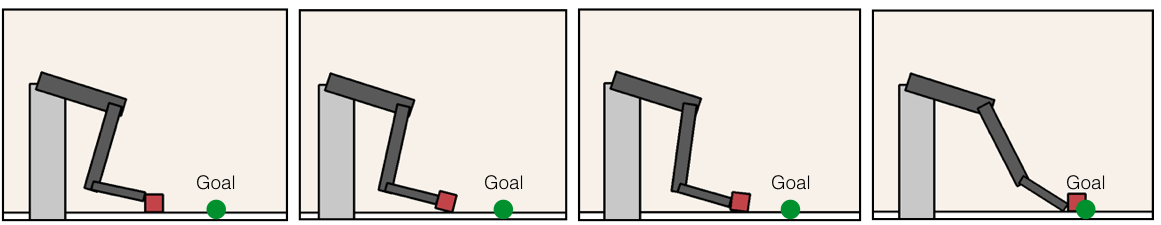
\includegraphics[width=\textwidth]{ddco-experiments/2d-sp-friction.png}
    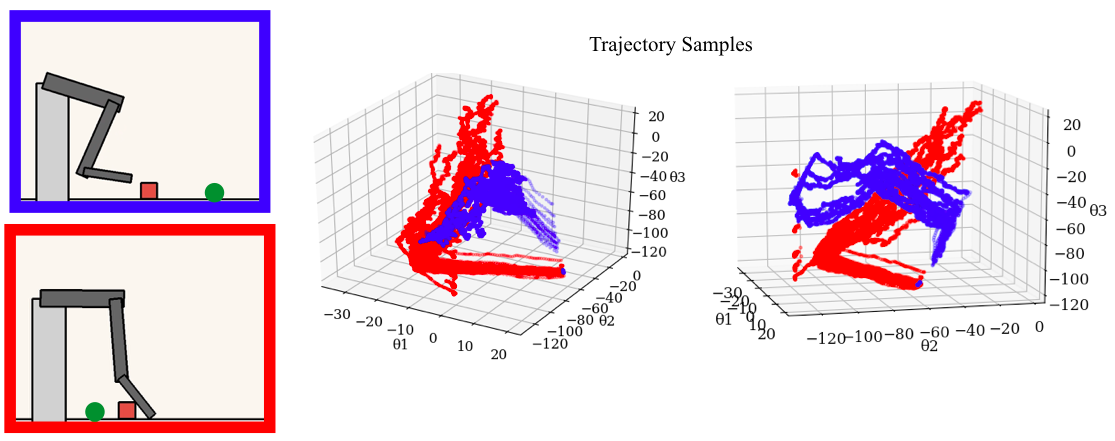
\includegraphics[width=\textwidth]{ddco-experiments/c-space.png}
    \caption{A 3-link robot arm has to push a box along a surface with friction to a randomly chosen goal state to the box's left or right without toppling it. Due to the collision and contact constraints of the 2D Surface Pushing task, it leads to two geometrically distinct pushing skills, backhand and forehand, for goals on the left and on the right. Right: 50 sampled trajectories from a motion-planning supervisor. \label{fig:b2dcspace}}
\end{figure}

Our algorithmic supervisor runs an RRT Connect motion planner (from the Open Motion Planning Library \textsf{ompl}) at each time-step planning till the goal. The motion planning algorithm contains a single important hyper-parameter which is the maximum length of branches to add to the tree. We set this at 0.1 units (for a 20 x 20 unit space). First, we consider the case where we observe the full low-dimensional state of the system: three joint angles, the box's position and orientation, and the position of the goal state. 
We compare our hierarchical policies with two flat, non-hierarchical policies. One baseline policy we consider is an under-parametrized linear policy which is not expressive enough to approximate the supervisor policy well. The other baseline policy is a multi-layer perceptron (MLP) policy.
We train each of these policies via Behavior Cloning (BC), i.e. by maximizing the likelihood each gives to the set of demonstrations.
As expected, the flat linear policy is unsuccessful at the task for any number of observed demonstrations (Figure \ref{fig:b2dexp1-1} Top-A). The MLP policy, on the other hand, can achieve the maximum reward when trained on 60 demonstrations or more. 

We apply \alg and learn two 2-level hierarchical policies, one with linear low-level options, and the other with MLP low-level options of the same architecture used for the flat policy. 

\vspace{0.25em}\noindent \textbf{Multi-Layer Perceptron Flat Policy: } One of the baseline policies is a multi-layer perceptron (MLP) policy which has a single ReLU hidden layer of 64 nodes.
This policy is implemented in Tensorflow and is trained with an ADAM optimizer with learning rate $1e-5$.

\vspace{0.25em}\noindent \textbf{\alg Policy 1: } In the first policy trained by \alg, we have a logistic regression meta-policy that selects from one of $k$ linear sub-policies. The linear sub-policies execute until a termination condition determined again by a logistic regression. This policy is implemented in Tensorflow and is trained with an ADAM optimizer with learning rate $1e-5$. For the linear hierarchy, we set \alg to discover 5 options, which is tuned using the cross-validation method described before.

\vspace{0.25em}\noindent \textbf{\alg Policy 2: } In the second policy trained by \alg, we have a logistic regression meta-policy that selects from one of $k$ multi-layer perceptron sub-policies. 
As with the flat policy, it has a single ReLU hidden layer of 64 nodes.
The MLP sub-policies execute until a termination condition determined again by a logistic regression. This policy is implemented in Tensorflow and is trained with an ADAM optimizer with learning rate $10^{-5}$. For the MLP hierarchy, we set \alg to discover 2 options, which is tuned using the cross-validation method described before.

In both cases, the termination conditions are parametrized by a logistic regression from the state to the termination probability, and the high-level policy is a logistic regression from the state to an option selection.
The MLP hierarchical policy can achieve the maximum reward with  30 demonstrations, and is therefore 2x more sample-efficient than its flat counterpart (Figure \ref{fig:b2dexp1-1} Top A).
We also vary the number of options discovered by \alg, and plot the reward obtained by the resulting policy (Figure \ref{fig:b2dexp1-1} Top-B). While the performance is certainly sensitive to the number of options, we find that the benefit of having sufficiently many options is only diminished gradually with each additional option beyond the optimum. Importantly, the peak in the cross-validated log-likelihood corresponds to the number of options that achieves the maximum reward (Figure \ref{fig:b2dexp1-1} Top-C). This allows us to use cross-validation to select the number of options without having to evaluate the policy by rolling it out in the environment.

\begin{figure}[ht!]
    \centering
    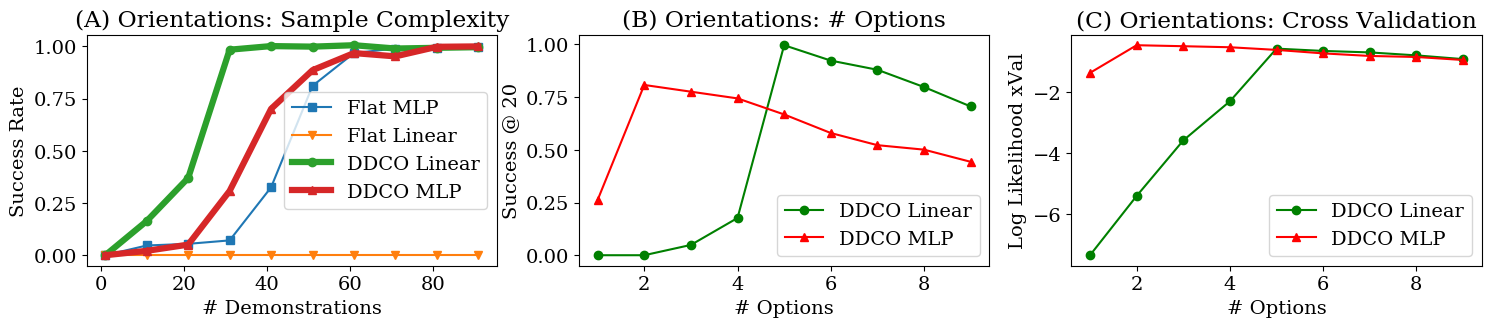
\includegraphics[width=\textwidth]{ddco-experiments/exp1-1.png}
    \caption{2D Surface Pushing from low-dimensional observations and image observations. (A) The sample complexity of different policy representations, (B) The success rate for different numbers of discovered options, (C) The peak in the reward correlates over the number of options with the 10-fold cross-validated log-likelihood. \label{fig:b2dexp1-1}}
\end{figure}

\vspace{0.25em}\noindent\textbf{Observing Images: } Next, we consider the case where the sensor inputs are 640x480 images of the scene. The low-dimensional state is still fully observable in these images, however these features are not observed explicitly, and must be extracted by the control policy. We consider two neural network architectures to represent the policy: a convolutional layer followed by either a fully connected layer or an LSTM, respectively forming a feed-forward (FF) network and a recurrent network (RNN).
We use these architectures both for flat policies and for low-level options in hierarchical policies.
For the hierarchical policies, as in the previous experiment, we consider a high-level policy that only selects options.
For the FF policy we discover 4 options, and for the RNN policy we discover 2 options.
 
 \vspace{0.25em}\noindent \textbf{\alg FF Policy: } First, we consider a neural network with a convolutional layer with 64 5x5 filters followed by a fully connected layer forming a feed-forward (FF) network. The high-level model only selects options and is parametrized by the same general architecture with an additional softmax layer after the fully connected layer. This means that the meta-control policy is a two-layer convolutional network whose output is a softmax categorical distribution over options. This policy is implemented in Tensorflow and is trained with an ADAM optimizer with learning rate $1e-5$.
 We used $k=2$ options for the FF policy.
 
 \vspace{0.25em}\noindent \textbf{\alg RNN Policy: } Next, we consider a neural network with a convolutional layer with 64 5x5 filters followed by an LSTM layer forming  a recurrent network (RNN). The high-level model only selects options and is parametrized by the same general architecture with an additional softmax layer after the LSTM. This policy is implemented in Tensorflow and is trained with a Momentum optimizer with learning rate $1e-4$ and momentum $4e-3$.
  We used $k=4$ options for the RNN policy.

  The hierarchical policies require 30\% fewer demonstrations than the flat policies to achieve the maximum reward (Figure \ref{fig:b2dexp1-1} Bottom-A).
Figure \ref{fig:b2dexp1-1} Bottom-B and C show how the success rate and cross-validated log-likelihood vary with the number of options.
As for the low-dimensional inputs, the success rate curve is correlated with the cross-validated log-likelihood.
We can rely on this to select the number of options offline without rolling out the learned hierarchical policy.

\begin{figure}[ht!]
    \centering
    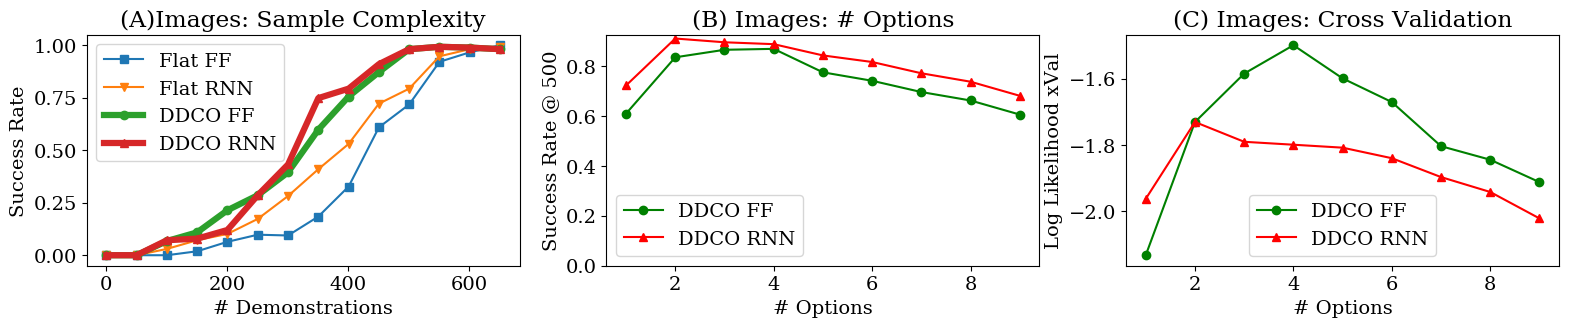
\includegraphics[width=\textwidth]{ddco-experiments/exp1-2.png}
    \caption{2D Surface Pushing from image observations and image observations. (A) The sample complexity of different policy representations, (B) The success rate for different numbers of discovered options, (C) The peak in the reward correlates over the number of options with the 10-fold cross-validated log-likelihood. \label{fig:b2dexp1-2}}
\end{figure}

\vspace{0.25em}\noindent\textbf{Control Space Augmentation (Kinematic): } 
We test two different architectures for the output layer of the high-level policy: either a softmax categorical distribution selecting an option, or the hybrid categorial--continuous distribution output described in~\sref{hybrid}.
The low-level policies are linear.

Figure \ref{fig:b2dexp1-3} describes the empirical estimation, through policy rollouts, of the success rate as a function of the number of options, and of the fraction of time that the high-level policy applies physical control.
When the options are too few to provide skills that are useful throughout the state space, physical controls can be selected instead to compensate in states where no option would perform well. This is indicated by physical control being selected with greater frequency. As more options allow a better coverage of the state space, the high-level policy selects physical controls less often, allowing it to generalize better by focusing on correct option selection. With too many discovered options, each option is trained from less data on average, making some options overfit and become less useful to the high-level policy.

\begin{figure}[ht!]
    \centering
    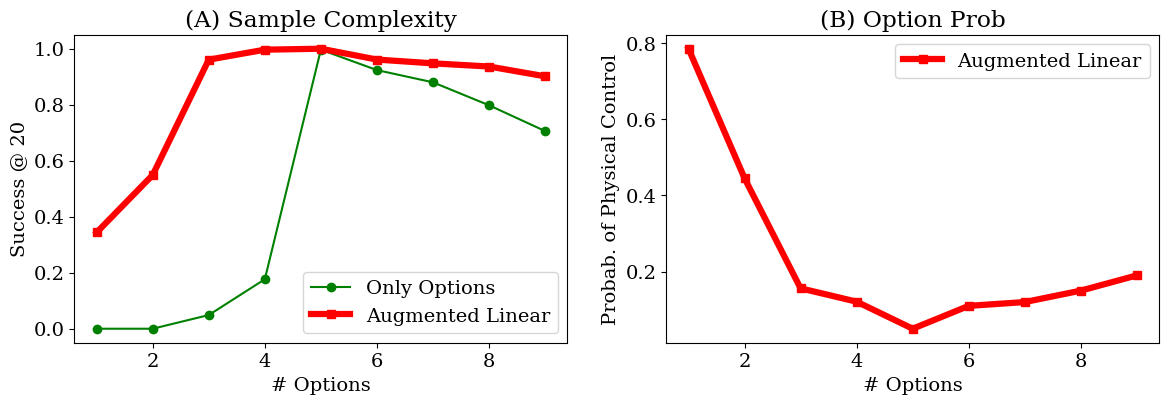
\includegraphics[width=\textwidth]{ddco-experiments/exp1-3.png}
    \caption{ (A) The sample complexity of augmented v.s. option-only high-level control spaces. (B) The fraction of high-level selections that are of physical control. The frequency of selecting a physical control first decreases with the number of options, then increases as options overfit. \label{fig:b2dexp1-3}}
\end{figure}


\vspace{0.25em}\noindent\textbf{Control Space Augmentation (Images): }  We ran the same experiment but on the image state-space instead of the low dimensional state.
The sensor inputs are 640x480 images of the scene and the task is the Box2D pushing task.
Figure \ref{fig:augimages} describes the empirical estimation, through policy rollouts, of the success rate as a function of the number of options, and of the fraction of time that the high-level policy applies physical control.
When the options are too few to provide skills that are useful throughout the state space, physical controls can be selected instead to compensate in states where no option would perform well. 

\begin{figure} [ht!]
\centering
    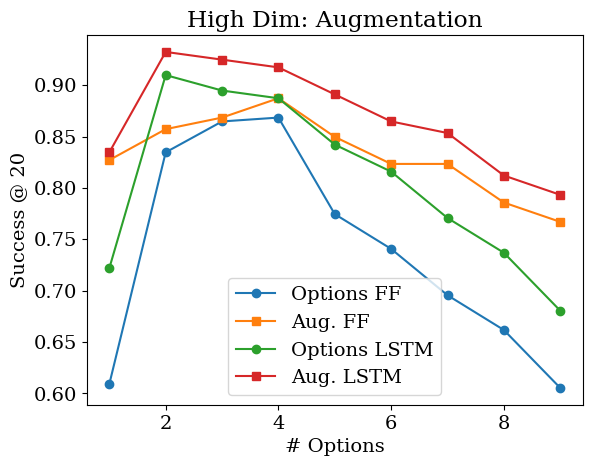
\includegraphics[width=0.4\textwidth]{ddco-experiments/exp7-1.png}
    \caption{Augmenting the action space instead of selecting only options with the meta-policy leads attenuates the losses when selecting too few or too many options. \label{fig:augimages}}
\end{figure}


\subsection*{Box2D Simulation: Discussion}
These results should be counterintuitive. While it is easy to reason about the low-dimensional kinematic case (where motions are essentially piecewise affine in the state), the results for image observations are less clear--why does hierarchy appear to help? 
To understand why, we ran a a follow up experiment. 
Figure \ref{fig:tsne} illustrates two plots color coded by kinematic class (forehand and backhand pushes).
The flat plot takes a TSNE visualizatio of the output first convolutional layer of the ``flat'' network and illustrates how the policy is structured. 
While there is clear structure, the \emph{same neuron are active for forehand motions and backhands}. On the other hand, when we visualize how the hierarchical policy partitions the trajectory space. It gives a cleaner seperation between the forehand and the backhand motions.
We speculate that while the action space is continuous there is a discontinuity in the set of actions relevant to the task due to the geometry and kinematic constraints.
The inherently discrete hierarchical representation captures this dicontinuity more accurately without a lot of data.

\begin{figure} [ht!]
\centering
    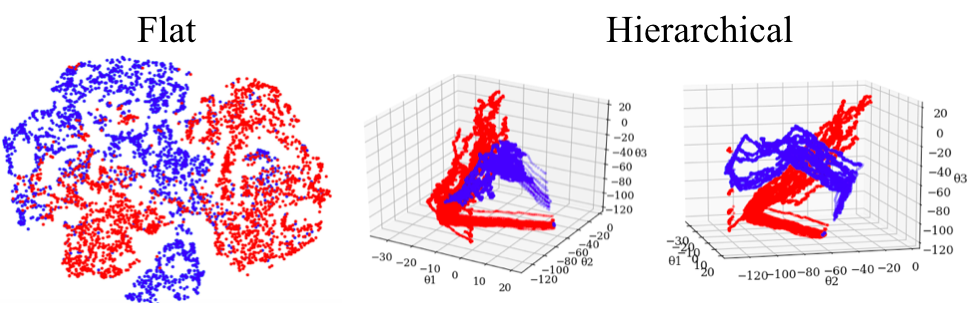
\includegraphics[width=\textwidth]{ddco-experiments/tsne.png}
    \caption{A visualization of how the flat and hierarchical policy seperate the space of observations. The flat policy is visualized with a tsne plot of its first\label{fig:tsne}}
\end{figure}

\subsection*{Physical Experiment 1: Needle Insertion}
We constructed a physical environment to replicate the simulation results on a real robotic platform.
We consider a needle orientation and insertion task on the da Vinci Research Kit (DVRK) surgical robot (Figure \ref{fig:dvrkexp3}). In this task, the robot must grasp a surgical needle, reorient it in parallel to a tissue phantom, and insert the needle into the tissue phantom.
The task is successful if the needle is inserted into a 1cm diameter target region on the phantom. Small changes in the needle's initial orientation can lead to large changes in the in-gripper pose of the needle due to deflection. 
The state is the current 6-DoF pose of the robot gripper, and algorithmically extracted visual features that describe the estimated pose of the needle.
These features are derived from an image segmentation that masks the needle from the background and fits an ellipsoid to the resulting pixels. 
The principal axis of this 2D ellipsoid is a proxy for the pose of the needle.
The task runs for a fixed 15 time-steps, and the policy must set the joint angles of the robot at each time-step.


\begin{figure}[ht!]
    \centering
    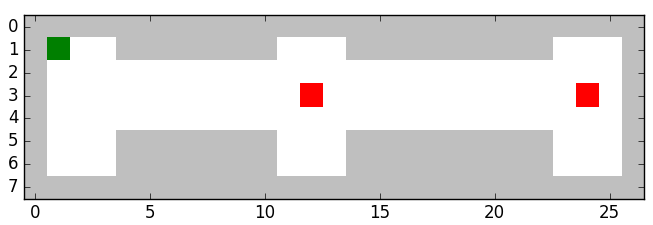
\includegraphics[width=\textwidth]{ddco-experiments/exp3.png}
    \caption{A needle orienting and insertion task. The robot must grasp a surgical needle, reorient it in parallel to a tissue phantom, and insert the needle.   \label{fig:dvrkexp3}}
\end{figure}

The needle's deflection coupled with the inaccurate kinematics of the DVRK make it challenging to plan trajectories to insert the needle properly.
A visual servoing policy needs to be trained that can both grasp the needle in the correct position, as well as reorient the gripper in the correct direction after grasping.
To collect demonstrations, we programmed an initial open-loop control policy, interrupted the robot via keyboard input when adjustment was needed, and kinesthetically adjusted the pose of the gripper. 
We collected 100 such demonstrations.

 We evaluated the following alternatives: (1) a single flat MLP policy with continuous output, (2) a flat policy consisting of 15 distinct MLP networks, one for each time-step, (3) a hierarchical policy with 5 options trained with \alg. We considered a hierarchy where the high-level policy is a MLP with a softmax output that selects the appropriate option, and each option is parametrized by a distinct MLP with continuous outputs.
 \alg learns 5 options, two of which roughly correspond to the visual servoing for grasping and lifting the needle, and the other three handle three different types of reorientation.
 For 100 demonstrations, the hierarchical policy learned with \alg has a 45\%  higher log-likelihood measured in cross-validation than the flat policy, and a 24\% higher log-likelihood than the per-timestep policy. 
 
\vspace{0.5em} \noindent \textbf{Task Description: } The robot must grasp a 1mm diameter surgical needle, re-orient it parallel to a tissue phantom, and insert the needle into a tissue phantom.
The task is successful if the needle is inserted into a 1 cm diameter target region on the phantom.
In this task, the state-space is the current 6-DoF pose of the robot gripper and visual features that describe the estimated pose of the needle.
These features are derived from an image segmentation that masks the needle from the background and fits an ellipsoid to the resulting pixels. 
The principal axis of this 2D ellipsoid is a proxy for the pose of the needle.
The task runs for a fixed 15 time-steps and the policy must set the joint angles of the robot at each time-step.

\vspace{0.5em} \noindent \textbf{Robot Parameters: } The challenge is that the curved needle is sensitive to the way that it is grasped. Small changes in the needle's initial orientation can lead to large changes to the in-gripper pose of the needle due to deflection.
This deflection coupled with the inaccurate kinematics of the DVRK leads to very different trajectories to insert the needle properly.

The robotic setup includes a stereo endoscope camera located 650 mm above the 10cm x 10 cm workspace.
After registration, the dvrk has an RMSE kinematic error of 3.3 mm, and for reference, a gripper width of 1 cm.
In some regions of the state-space this error is even higher, with a 75\% percentile error of 4.7 mm.
The learning in this task couples a visual servoing policy to grasp the needle with the decision of which direction to orient the gripper after grasping.

\vspace{0.5em} \noindent \textbf{Demonstration Protocol: }
To collect demonstrations, we programmed an initial open-loop control policy. This policy traced out the basic desired robot motion avoiding collisions and respecting joint limits, and grasping at where it believed the needle was and an open-loop strategy to pin the needle in the phantom.
This was implemented by 15 joint angle way points which were interpolated by a motion planner.
We observed the policy execute and interrupted the robot via keyboard input when adjustment was needed.
This interruption triggered a clutching mechanism and we could 
kinesthetically adjusted the joints of the robot and pose of the gripper (but not the open-close state).
The adjustment was recorded as a delta in joint angle space which was propagated through the rest of the trajectory.
We collected 100 such demonstrations and images of these adjustments are visualized in image (Figure \ref{fig:demo}).

  \begin{figure}[ht!]
    \centering
    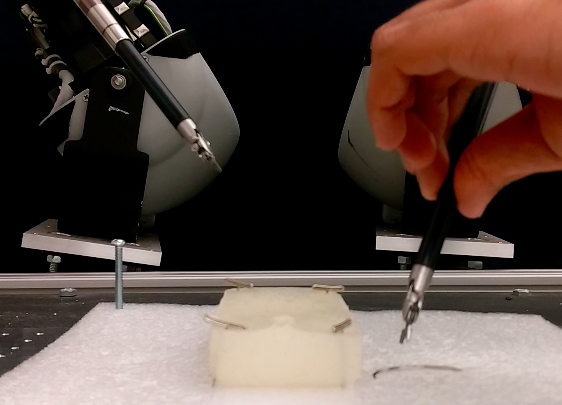
\includegraphics[width=0.48\textwidth]{ddco-experiments/demo-1.png}
    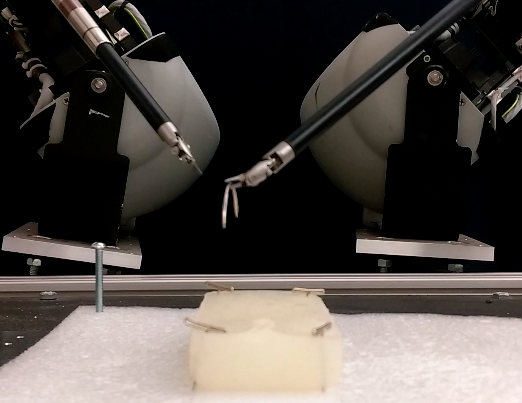
\includegraphics[width=0.455\textwidth]{ddco-experiments/demo-2.png}
    \caption{To collect demonstrations, we programmed an initial open-loop control policy. We observed the policy execute and interrupted the robot via keyboard input when adjustment was needed.  \label{fig:demo}}
\end{figure}


\vspace{0.25em} \noindent \textbf{Learning the Parameters: } Figure \ref{fig:dvrkexp1}A plots the cross-validation log-likelihood as a function of the number of demonstrations.
We find that the hierarchical model has a higher likelihood than the alternatives---meaning that it more accurately explains the observed data and generalizes better to held out data.
At some points, the relative difference is over 30\%.
It, additionally, provides some interpretability to the learned policy.
Figure \ref{fig:dvrkexp1}B visualizes two representative trajectories.
We color code the trajectory based on the option active at each state (estimated by \alg).
The algorithm separates each trajectory into 3 segments: needle grasping, needle lifting, and needle orienting.
The two trajectories have the same first two options but differ in the orientation step.
One of the trajectories has to rotate in a different direction to orient the needle before insertion.

\begin{figure}[ht!]
    \centering
    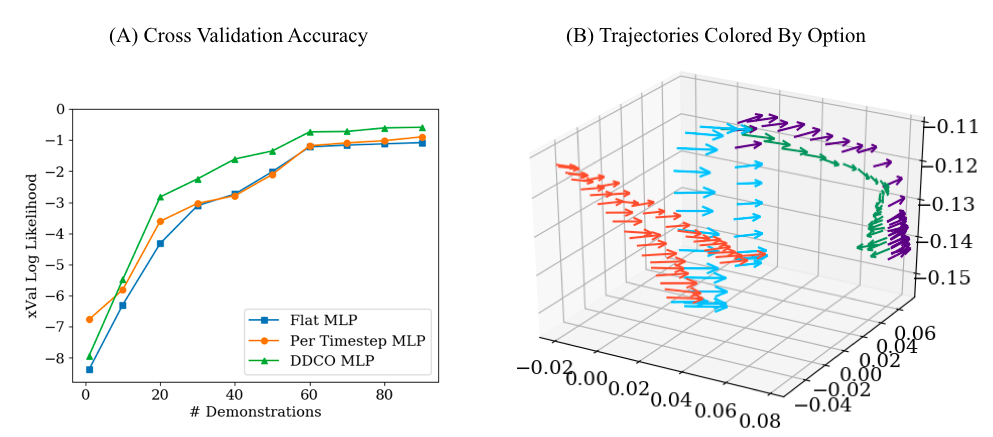
\includegraphics[width=\textwidth]{ddco-experiments/exp-5-1-1.png}
    \caption{(A) We plot the cross validation likelihood of the different methods as a function of the number of demonstrations. (B) We visualize two representative trajectories (position and gripper orientation) color coded by the most likely option applied at that timestep. We find that the two trajectories have the same first two options but then differ in the final step due to the re-orientation of the gripper before insertion.  \label{fig:dvrkexp1}}
\end{figure}


\vspace{0.25em} \noindent \textbf{Flat Policy: } One of the baseline policies is a multi-layer perceptron (MLP) policy which has a single ReLU hidden layer of 64 nodes.
This policy is implemented in Tensorflow and is trained with an ADAM optimizer with learning rate $1e-5$.

\vspace{0.25em} \noindent \textbf{Per-Timestep Policy: } Next, we consider a degenerate case of options where each policy executes for a single-timestep. We train 15 distinct multi-layer perceptron (MLP) policies each of which has a single ReLU hidden layer of 64 nodes.
Thes policies are implemented in Tensorflow and are trained with an ADAM optimizer with learning rate $1e-5$.

\vspace{0.25em} \noindent \textbf{\alg Policy: } \alg trains a hierarchical policy with 5 options. We considered a hierarchy where the meta policy is a multilayer perceptron with a softmax output that selects the appropriate option, and the options are parametrized by another multilayer perceptron with continuous outputs. Each of the MLP policies has a single ReLU hidden layer of 64 nodes.
Thes policies are implemented in Tensorflow and are trained with an ADAM optimizer with learning rate $1e-5$.


\vspace{0.25em} \noindent \textbf{Execution: } 
For each of the methods, we execute ten trials and report the success rate (successfully grasped and inserted the needle in the target region), and the accuracy.
The results are described in aggregate in the table below:

\begin{table}[ht!]\footnotesize
\centering
\label{my-label}
\begin{tabular}{l|l|l|l|l|}
             & Overall Success & Grasp Success & Insertion Success & Insertion Accuracy \\
             \hline
Open Loop    & 2/10   & 2/10  & 0/0 & $7 \pm 1$ mm                  \\
Behavioral Cloning & 3/10 & 6/10  & 3/6 &   $6 \pm 2$ mm     \\
Per Timestep & 6/10  & 7/10  & 6/7 &   $5 \pm 1$ mm \\ 
\alg & 8/10 & 10/10 & 8/10 &  $5 \pm 2$ mm  \\
\end{tabular}
\end{table}

We ran preliminary trials to confirm that the trained options can be executed on the robot.
For each of the methods, we report the success rate in 10 trials, i.e. the fraction of trials in which the needle was successfully grasped and inserted in the target region. %We also report the insertion accuracy.
All of the techniques had comparable accuracy in trials where they successfully grasped and inserted the needle into the 1cm diameter target region.
The algorithmic open-loop policy only succeeded 2/10 times.
Surprisingly, Behavior Cloning (BC) did not do much better than the open-loop policy, succeeding only 3/10 times.
Per-timestep BC was far more successful (6/10).
Finally, the hierarchical policy learned with \alg succeeded 8/10 times. On 10 trials it was successful 5 times more than the direct BC approach and 2 times more than the per-timestep BC approach.
While not statistically significant, our preliminary results suggest that hierarchical imitation learning is also beneficial in terms of task success, in addition to improving model generalization and interpretability.

\begin{figure}[ht!]
    \centering
    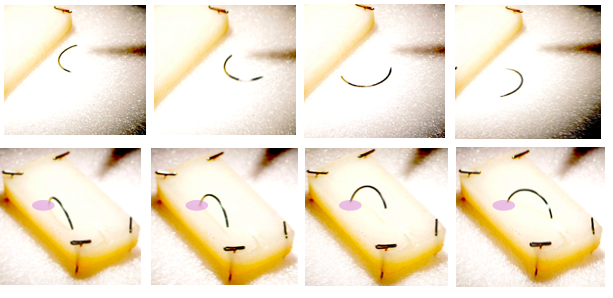
\includegraphics[width=\textwidth]{ddco-experiments/exp3-1.png}
    \caption{Illustration of the needle orientation and insertion task. Above are images illustrating the variance in the initial state, below are corresponding final states after executing \alg.  \label{fig:dvrkexp3-1}}
\end{figure}


\begin{figure}[ht!]
    \centering
    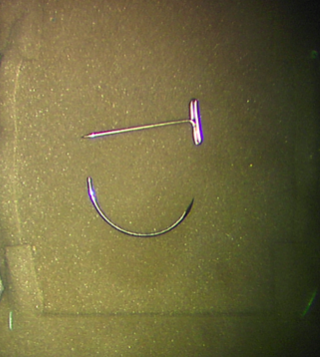
\includegraphics[width=0.25\textwidth]{ddco-experiments/image.png}
    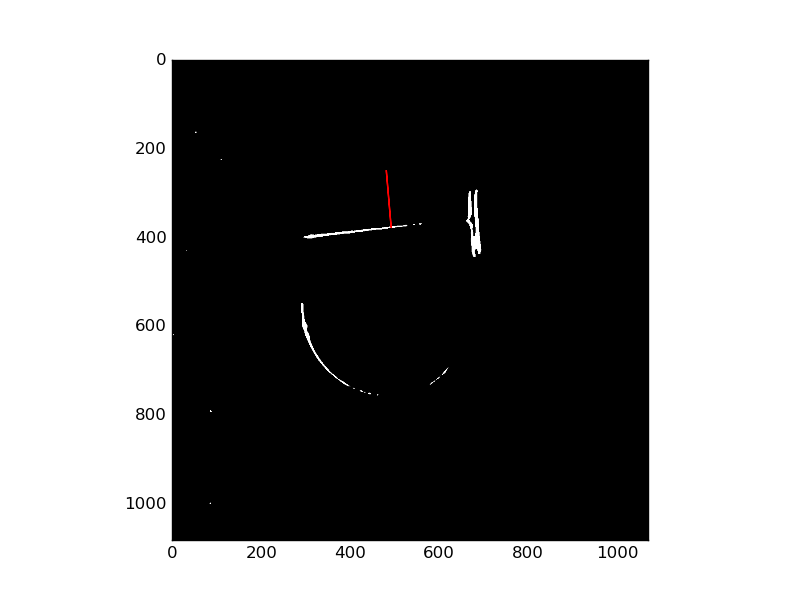
\includegraphics[width=0.4\textwidth]{ddco-experiments/binary-mask.png}
    \caption{The endoscope image and a corresponding binary mask with a selected grasp. The arrow corresponds to the orientation of the gripper along the grasp axis.  \label{fig:dvrkim}}
\end{figure}


\subsection*{Physical Experiment 2: Surgical Bin Picking}
In this task, the robot is given a foam bin with a pile of 5--8 needles of three different types, each 1--3mm in diameter.
The robot must extract needles of a specified type and place them in an ``accept'' cup, while placing all other needles in a ``reject'' cup.
The task is successful if the entire foam bin is cleared into the correct cups.

In initial trials, the kinematics of the DVRK were not precise enough for grasping needles.
We then realized that visual servoing is needed, which requires learning.
However, even with visual servoing, failures are common, and we would like to also learn automatic recovery behaviors. 
To define the state space for this task, we first generate binary images from overhead stereo images, and apply a color-based segmentation to identify the needles (the \textsf{image} input).
Then, we use a classifier trained in advance on 40 hand-labeled images to identify and provide a candidate grasp point, specified by position and direction in image space (the \textsf{grasp} input). 
Additionally, the 6 DoF robot gripper pose and the open-closed state of the gripper are observed (the \textsf{kin} input).
The state space of the robot is (\textsf{image}, \textsf{grasp}, \textsf{kin}), and the control space is the 6 joint angles and the gripper angle.

Each sequence of grasp, lift, move, and drop operations is implemented in 10 control steps of joint angle positions.
As in the previous task,  we programmed an initial open-loop control policy, interrupted the robot via keyboard input when adjustment was needed, and kinesthetically adjusted the pose of the gripper. 
We collected 60 such demonstrations, in each fully clearing a pile of 3--8 needles from the bin, for a total of 450 individual grasps.


\begin{figure}[ht!]
    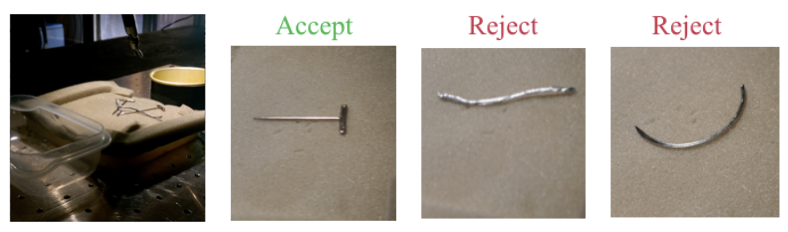
\includegraphics[width=0.58\textwidth]{ddco-experiments/needle-sorting2.png}
    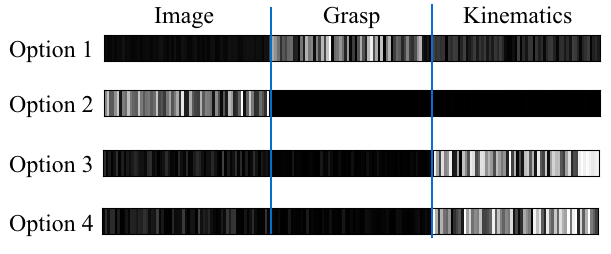
\includegraphics[width=0.4\textwidth]{ddco-experiments/ReLU-dvrk-options.png}
    \caption{(Left) Surgical Bin Picking: the robot is given a foam bin with a pile of 5--8 needles of three different types, each 1--3mm in diameter. The robot must extract needles of a specified type and place them in an ``accept'' cup, while placing all other needles in a ``reject'' cup. (Right) For each of the 4 options, we plot how heavily the different inputs are weighted (\textsf{image}, \textsf{grasp}, or \textsf{kin}) in computing the option's action. Nonzero values of the ReLU units are marked in white and indicate input relevance. \label{fig:dvrkexp4}} 
\end{figure}


We apply \alg to the collected demonstrations with the policy architecture described in \textbf{SM 1.4}. In this network, there are three inputs: a binary \textsf{image}, a candidate \textsf{grasp}, and kinematics (\textsf{kin}). These inputs are processed by distinct branches of the network before being aggregated into a single feature layer.  Using the cross-validation technique described in~\sref{k-validation}, we selected the number of options to be $k=4$.

We plot the average activations of the feature layer for each low-level option (Figure \ref{fig:dvrkexp4}). While this is only a coarse analysis, it gives some indication of which inputs (\textsf{image}, \textsf{grasp}, or \textsf{kin}) are relevant to the policy and termination. We see that the options are clearly specialized. The first option has a strong dependence only on the \textsf{grasp} candidate, the second option attends almost exclusively to the \textsf{image}, while the last two options rely mostly on \textsf{kin}.
The experimental details are described below:

\vspace{0.5em} \noindent \textbf{Task Description: } We consider a task with a more complicated high-level structure.
In this task, the robot is given a foam bin with 3 different types of needles (1mm-3mm in diameter) lying in a pile (5-8 needles in experiments).
The robot must extract a particular type of needle  and place it in the accept cup and place all others in a reject cup.
The task is successful if the entire foam bin is cleared.

Figure \ref{fig:dvrkcats} shows representive objects for this task. We consider three types of ``needles'': dissection pins, suturing needles, and wires.
Dissection pins are placed in the accept cup and the other two are placed in the reject cup.


\vspace{0.5em} \noindent \textbf{Robot and State-Space Parameters: } As in the previous task, the task requires learning because the kinematics of the dvrk are such that the precision needed for grasping needles requires visual servoing.
However, even with visual servoing, failures are common due to the pile (grasps of 2, 3, 4 objects).
We would like to automatically learn recovery behaviors. 
In our robotic setup, there is an overhead endoscopic stereo camera, and it is located 650mm above the workspace.

To define the state-space for this task, we first generate binary images from the stereo images and apply a color-based segmentation to identify the needles (we call this feature \textsf{image}).
Then, we use a classifier derived from 40 hand-labeled images to identify possible grasp points to sample a candidate grasp ( left pixel value, right pixel value, and direction) (we call this feature \textsf{grasp}). 
These features are visualized in Figure \ref{fig:dvrkim}.
Additionally, there is the 6 DoF robot gripper pose and the open-close state of the gripper (we call this feature \textsf{kin}).
The state-space of the robot is (\textsf{kin}, \textsf{image}, \textsf{grasp}), and the action space for the robot is 6 joint angles and the gripper angle.
Each grasp, lift, move, and drop operation consists of 10 time steps of joint angle positions. The motion between the joint angles is performed using a SLURP-based motion planner.

\begin{figure}[ht!]
    \centering
    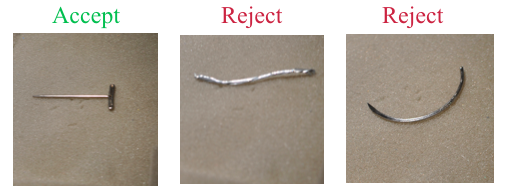
\includegraphics[width=\textwidth]{ddco-experiments/bin-picking-cats.png}
    \caption{There are two bins, one accept and one reject bin. In the accept bin, we place dissection pins and place the suturing needles and the wires in the other. \label{fig:dvrkcats}}
\end{figure}

\vspace{0.5em} \noindent \textbf{Demonstration Protocol: } As in the previous task, to collect demonstrations, we start with a hard-coded open-loop policy.
We roll this policy out and interrupt the policy when we anticipate a failure.
Then, we kinesthetically adjust the pose of the dvrk and it continues.
We collected 60 such demonstrations of fully clearing the bin filled with 3 to 8 needles each--corresponding to 450 individual grasps.
We also introduced a key that allows the robot to stop in place and drop it current grasped needle.
Recovery behaviors were triggered when the robot grasps no objects or more than one object.
Due to the kinesthetic corrections, a very high percentage of the attempted grasps (94\%) grasped at least one object. 
Of the successful grasps, when 5 objects are in the pile 32\% grasps picked up 2 objects, 14\% picked up 3 objects, and 0.5\% picked up 4.
In recovery, the gripper is opened and the epsiode ends leaving the arm in place.
The next grasping trial starts from this point.


\begin{figure} [ht!]
    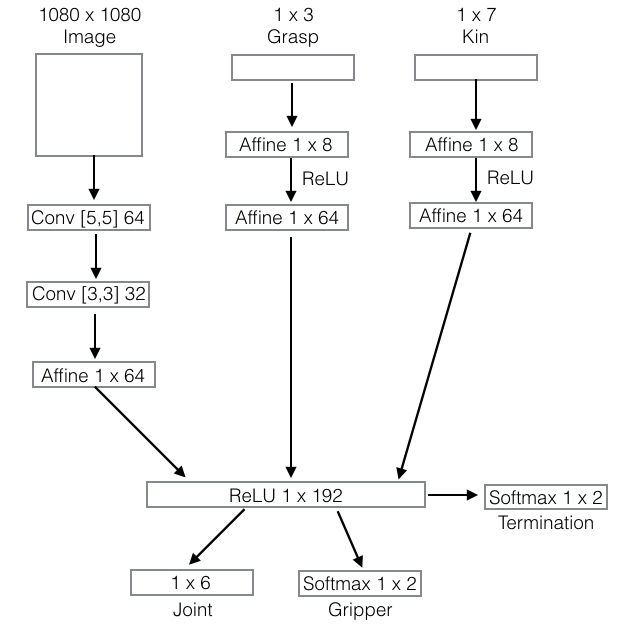
\includegraphics[width=0.48\textwidth]{ddco-experiments/net.png}
    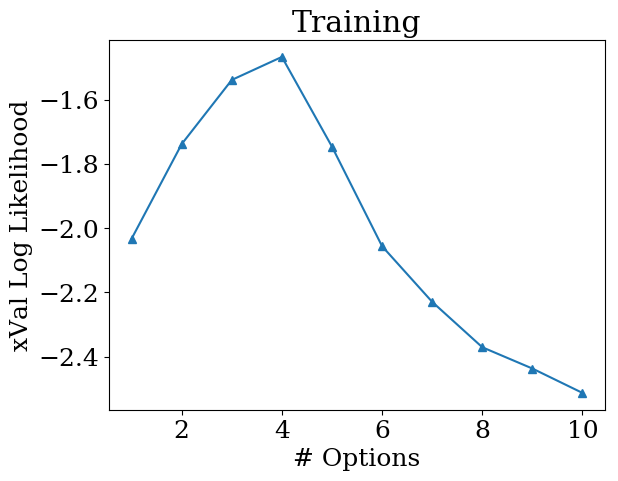
\includegraphics[width=0.48\textwidth]{ddco-experiments/exp6-1.png}
    \caption{We use the above neural network to parametrize each of the four options learned by \alg. In this network, there are three inputs the a binary image, a candidate grasp, and kinematics. These inputs are processed through individual neural net branches and aggregated into a single output layer. This output layer sets the joint angles of the robot and the gripper state (open or closed). Option termination is also determined from this output. \label{fig:dvrknet}}
\end{figure}

\vspace{0.25em} \noindent \textbf{Policy Parametrization: } We apply \alg to the collected demonstrations with the policy parametrization described in Figure \ref{fig:dvrknet}. In this network, there are three inputs the a binary image, a candidate grasp, and kinematics. These inputs are processed through individual neural net branches and aggregated into a single output layer. This output layer sets the joint angles of the robot and the gripper state (open or closed). Option termination is also determined from this output. Using the cross-validation technique described in before, we identify 4 options (Figure \ref{fig:dvrknet}). The high-level policy has the same parametrization but after the output layer there is a softmax operation that selects a lower-level option.  

\begin{figure} [ht!]
    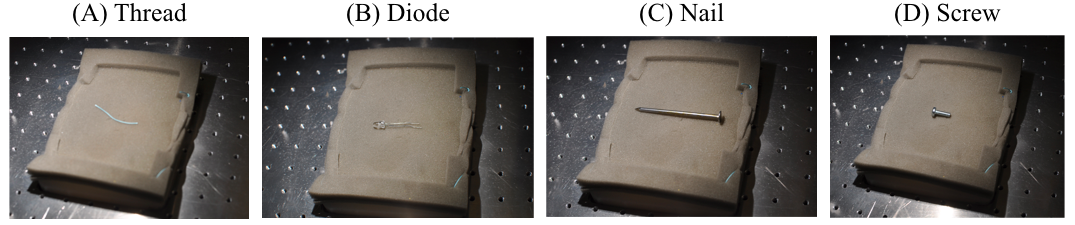
\includegraphics[width=\textwidth]{ddco-experiments/unseen.png}
    \caption{We evaluated the generalization of the learned policy on a small set of unseen objects. This was to understand what features of the object binary mask is used to determine behaviors.\label{fig:dvrkgen}}
\end{figure}

\vspace{0.25em} \noindent \textbf{Coordinate Systems: } We also experimented with different action space representations to see if that had an effect on single object grasps and categorizations. We trained alternative policies with the collected dataset where instead of predicting joint angles, we alternatively predicted 6 DoF end-effector poses with a binary gripper open-close state , and end-effector poses represented a rotation/translation matrix with a binary gripper open-close state. 
We found that the joint angle representation was the most effective. 
In particular, we found that for the grasping part of the task, a policy that controlled the robot in terms of tooltip poses was unreliable.

\begin{table}[ht!]\footnotesize
\centering
\label{my-label}
\begin{tabular}{l|l|l|l|l|}
       & Items & Successful Grasp & Successful Recovery & Successful Categorizations \\
       \hline
Joint Angle & 8     & 7/8         & 2/2    & 7/7                         \\
Tooltip Pose  & 8     & 3/8         & 5/5    & 3/3                             \\
Rotation   & 8     & 2/8          & 0/8    & 0                     
\end{tabular}
\end{table}
\begin{figure} [ht!]
\centering
    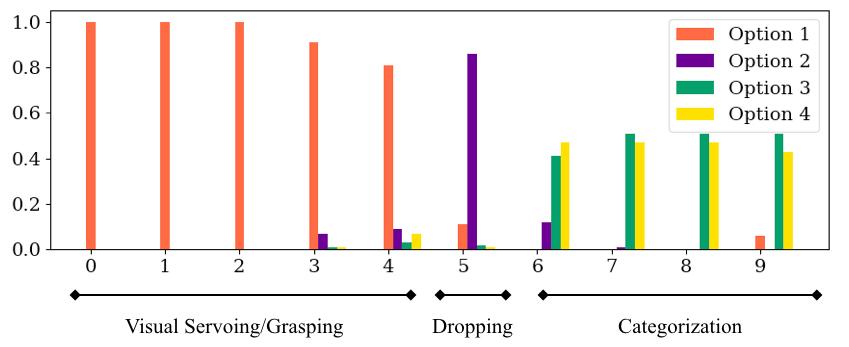
\includegraphics[width=0.8\textwidth]{ddco-experiments/highlevel-options.png}
    \caption{We plot the time distribution of the options selected by the high-level policy. The x-axis represents time, and the bars represent the probability mass assigned to each option. We find that the structure of the option aligns with key phases in the task such as servoing to the needle, grasping it, and categorizing. \label{fig:dvrkhl}}
\end{figure}

\vspace{0.25em} \noindent \textbf{Interpreting Learned Options: }
We additionally analyzed the learned options to see if there was an interpretable structure.
We examined the collected demonstrations and looked at the segmentation structure.
We average over the 60 trials the probability for the high-level policy to choose each option in each of first 10 time-steps during training (Figure \ref{fig:dvrkhl}). We find that the options indeed cluster visited states and segment them in alignment with key phases in the task, such as servoing to the needle, grasping it, dropping it if necessary, and categorizing it into the accept cup. 

\vspace{0.25em} \noindent \textbf{Full Break Down of Experimental Results: }
In 10 trials, 7 out of 10 were successful (Table \ref{big-experiment}). The main failure mode was unsuccessful grasping (defined as either no needles or multiple needles). As the piles were cleared and became sparser, the robot's grasping policy became somewhat brittle. The grasp success rate was 66\% on 99 attempted grasps. In contrast, we rarely observed failures at the other aspects of the task. Of the grasps that failed, nearly 34\% were due to grasping multiple objects.


\begin{table*}[ht!]\footnotesize
\centering
\label{big-experiment}
\begin{tabular}{l|l|l|l|l|l|}
{Trial \#} & { \# of Needles} & { \# Needles Cleared} & { Grasping} & { Recovery} & { Categorization} \\
\hline
1                               & 6                                    & {\color[HTML]{32CB00} \textbf{6}}         & 6/9                             & 3/3                             & 6/6                                   \\
2                               & 8                                    & 6                                         & 7/12                            & 5/6                             & 6/7                                   \\
3                               & 7                                    & {\color[HTML]{32CB00} \textbf{7}}         & 7/8                             & 1/1                             & 7/7                                   \\
4                               & 6                                    & {\color[HTML]{32CB00} \textbf{6}}         & 6/10                            & 4/4                             & 6/6                                   \\
5                               & 7                                    & 6                                         & 6/11                            & 5/5                             & 6/6                                   \\
6                               & 8                                    & {\color[HTML]{32CB00} \textbf{8}}         & 8/13                            & 5/5                             & 8/8                                   \\
7                               & 6                                    & 5                                         & 5/9                             & 4/4                             & 5/5                                   \\
8                               & 7                                    & {\color[HTML]{32CB00} \textbf{7}}         & 7/10                            & 3/3                             & 7/7                                   \\
9                               & 8                                    & {\color[HTML]{32CB00} \textbf{8}}         & 8/10                            & 2/2                             & 8/8                                   \\
10                              & 6                                    & {\color[HTML]{32CB00} \textbf{6}}         & 6/7                             & 1/1                             & 6/6                                   \\
Totals                          & 69                                   & Success: 70\%                             & Success: 66\%                   & Success: 97\%                   & Success: 98\%                        
\end{tabular}
\end{table*}



\vspace{0.25em} \noindent \textbf{Generalization to unseen objects: } We also evaluated the learned policy on a few unseen objects (but similarly sized and colored) to show that there is some level of generalization in the learning. We tried out four novel objects and evaluated what the learned policy did for each (Figure \ref{fig:dvrkgen}). For each of the novel objects we tried out 10 grasps in random locations and orientations in the bin (without any others). We evaluated the grasp success and whether it was categorized consistently (i.e., does the learned policy consistently think it is a pin or a needle).

We found that the diode was consistently grasped and categorized as a dissection pin. We conjecture this is because of its head and thin metallic wires. On the other hand, the screw and the thread were categorized in the reject cup. For 8/10 of the successful grasps, the nail was categorized as a failure mode. We conjucuture that since it is the large object it looks similar to the two object grasps seen in the demonstrations.

% Please add the following required packages to your document preamble:
% \usepackage[normalem]{ulem}
% \useunder{\uline}{\ul}{}
\begin{table}[ht!]\footnotesize
\centering
\label{my-label}
\begin{tabular}{l|l|l|l|l|l}
       & Grasps & Successful & Drop & Categorize Accept & Categorize Reject \\
       \hline
Thread & 10     & 10         & 1    & 0              & 9                 \\
Diode  & 10     & 10         & 0    & 10             & 0                 \\
Nail   & 10     & 8          & 8    & 0              & 0                 \\
Screw  & 10     & 4          & 0    & 0              & 4                
\end{tabular}
\end{table}


Finally, we evaluate the success of the learned hierarchical policy in 10 full trials, according to 4 different success criteria. First, the overall task success is measured by the success rate of fully clearing the bin without failing 4 consecutive grasping attempts. Second, we measure the success rate of picking exactly one needle in individual grasp attempts. Third, we measure the success rate of appropriately reacting to grasps, by dropping the load and retrying unsuccessful grasps, and not dropping successful grasps. Fourth, we measured the success rate of needle categorization.

In 10 trials, 7/10 were successful. The main failure mode was unsuccessful grasping due to picking either no needles or multiple needles. As the piles were cleared and became sparser, the robot's grasping policy became somewhat brittle. The grasp success rate was 66\% on 99 attempted grasps. In contrast, we rarely observed failures at the other aspects of the task, reaching 97\% successful recovery on 34 failed grasps. 


\subsection*{Vector Quantization For Initialization}
One challenge with \alg is initialization.
When real perceptual data is used, if all of the low-level policies initialize randomly the forward-backward estimates needed for the Expectation-Gradient will be poorly conditioned where there is an extremely low likelihood assigned to any particular observation.
The EG algorithm relies on a segment-cluster-imitate loop, where initial policy guesses are used to segment the data based on which policy best explains the given time-step, then the segments are clustered, and the policies are updated.
In a continuous control space, a randomly initialized policy may not explain any of the observed data well.
This means the small differences in initialization can lead to large changes in the learned hierarchy.

We found that a necessary pre-processing step was a variant of vector quantization, originally proposed for problems in speech recognition. 
We first cluster the state observations using a \textsf{k-means} clustering and train $k$ behavioral cloning policies for each of the clusters.
We use these $k$ policies as the initialization for the EG iterations.
Unlike the random initialization, this means that the initial low level policies will demonstrate some preference for actions in different parts of the state-space.
We set $k$ to be the same as the $k$ set for the number of options, and use the same optimization parameters.

\subsection*{Layer-wise Hierarchy Training}
We also found that layer-wise training of the hierarchy greatly reduced the likelihood of a degenerate solution.
While, at least in principle, one can train 
When the meta-policy is very expressive and the options are initialized poorly, sometimes the learned solution can degenerate to excessively using the meta-policy (high-fitting). 
We can avoid this problem by using a simplified parametrization for the meta-control policy $\eta_d$ used when discovering the low-level options. For example, we can fix a uniform meta-control policy that chooses each option with probability $\nicefrac 1 {k}$. Now, once these low-level options are discovered, then we can augment the action space with the options and train the meta-policy.

This same algorithm can recursively proceed to deep hierarchies from the lowest level upward: level-$d$ options can invoke already-discovered lower-level options; and are discovered in the context of a simplified level-$d$ meta-control policy, decoupled from higher-level complexity.
Perhaps counter-intuitively, this layer-wise training does not sacrifice too much during option discovery, and in fact, initial results seem to indicate that it improves the stability of the algorithm.
An informative meta-control policy would serve as a prior on the assignment of demonstration segments to the options that generated them, but with sufficient data this assignment can also be inferred from the low-level model, purely based on the likelihood of each segment to be generated by each option.

\begin{figure} [ht!]
\centering
    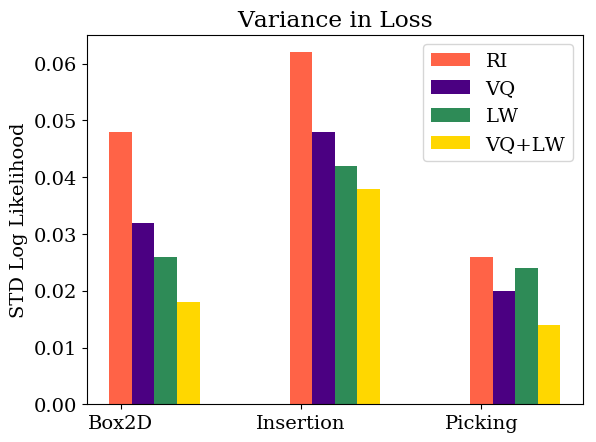
\includegraphics[width=0.3\textwidth]{ddco-experiments/exp8-1.png}
    \caption{This experiment measures the variance in log likelihood over 10 different runs of \alg with different training and initialization strategies. Vector Quantization (VQ) and Layer-Wise training (LW) help stabilize the solution. \label{fig:exp81}}
\end{figure}


\subsection*{Results: Stability of \alg}
In the first experiment, we measure the variance in log likelihood over 10 different runs of \alg with different training and initialization strategies (Figure \ref{fig:exp81}). 
We use the entire datasets presented before and use the FF architecture for the Box2D experiments.
Vector Quantization (VQ) and Layer-Wise training (LW) help stabilize the solution and greatly reduce the variance of the algorithm.
This reduction in variance is over 50\% in the Box2D experiments, and a little more modest for the real data.

In the next experiment, we measure the consistency of the solutions found by \alg (Figure \ref{fig:exp82}).
For each of the demonstration trajectories, we annotate the time-step by the most likely option.
One can view this annotation as a hard clustering of the state-action tuples.
Then, we measure the average normalized mutual information (NMI) between all pairs of the 10 different runs of \alg.
NMI is a measure of how aligned two clusterings are between 0 and 1, where 1 indicates perfect alignment.
As with the likelihood, Vector Quantization (VQ) and Layer-Wise training (LW) significantly improve the consistency of the algorithm.


In the last experiment, we measure the symptoms of the ``high-fitting'' problem (Figure \ref{fig:exp83}).
We plot the probability that the high-level policy selects an option.
In some sense, this measures how much control the high-level policy delegates to the options.
Surprisingly, VQ and LW have an impact on this.
Hierarchies trained with VQ and LW have a greater reliance on the options.

\begin{figure} [ht!]
\centering
    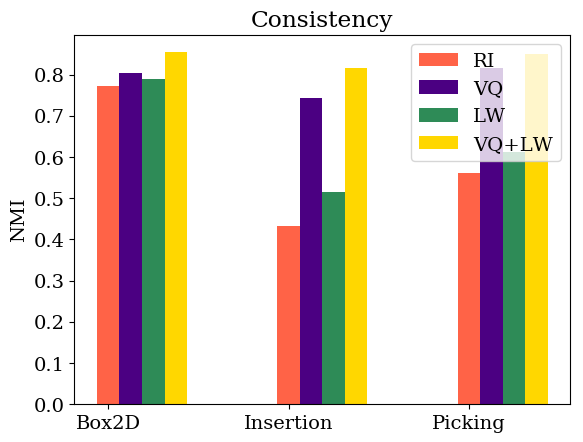
\includegraphics[width=0.5\textwidth]{ddco-experiments/exp8-2.png}
    \caption{We measure the average normalized mutual information between multiple runs of \alg. This measures the consistency of the solutions across intializations. \label{fig:exp82}}
\end{figure}


\begin{figure} [ht!]
\centering
    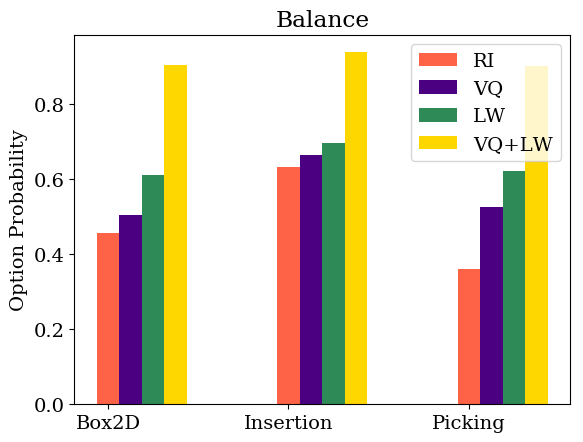
\includegraphics[width=0.5\textwidth]{ddco-experiments/exp8-3.png}
    \caption{We measure probability that an option is selected by the high-level policy. \label{fig:exp83}}
\end{figure}

\subsection*{The Effects of Dropout}
For the real datasets, we leverage a technique called dropout, which has been widely used in neural network training to prevent overfitting.
Dropout is a technique that randomly removes a unit from
the network along with all its connections.
We found that this technique improved performance when the datasets were small. We set the dropout parameter to 0.5 and measured the performance on a hold out set.
We ran an experiment on the needle insertion task dataset, where we measured the cross-validation accuracy on held out data with and without dropout (Figure \ref{fig:exp9}).
Dropout seems to have a substantial effect on improving cross-validation accuracy on a hold out set.

\begin{figure} [ht!]
\centering
    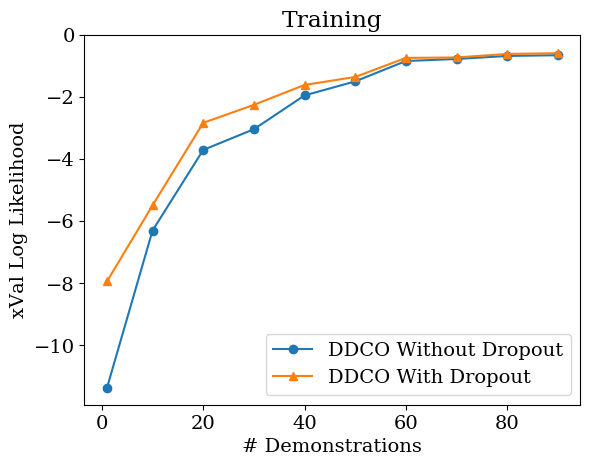
\includegraphics[width=0.4\textwidth]{ddco-experiments/exp9.png}
    \caption{Dropout seems to have a substantial effect on improving cross-validation accuracy on a hold out set. \label{fig:exp9}}
\end{figure}

\section{Segmentation of Robotic-Assisted Surgery}
In this section, we illustrate the wide applicability of the \alg framework by applying it to human demonstrations in a robotic domain. We apply \alg to long robotic trajectories (e.g. 3 minutes) demonstrating an intricate task, and discover options for useful subtasks, as well as segmentation of the demonstrations into semantic units.
The JIGSAWS dataset consists of surgical robot trajectories of human surgeons performing training procedures~\cite{gao2014jigsaws}. 
The dataset was captured using the da Vinci Surgical System from eight surgeons with different skill levels, performing five repetitions each of \emph{needle passing}, \emph{suturing}, and \emph{knot tying}.
This dataset consists of videos and kinematic data of the robot arms, and is annotated by experts identifying the activity occurring in each frame.

Each policy network takes as input a three-channel RGB $200 \times 200$ image, downscaled from $640 \times 480$ in the dataset, applies three convolutional layers with ReLU activations followed by two fully-connected dense layers reducing to $64$ and then eight real-valued components. An action is represented by 3D translations and the opening angles of the left and right arm grippers.

We investigate how well the segmentation provided by \alg corresponds to expert annotations, when applied to demonstrations of the three surgical tasks. Figure \ref{surgery-1} shows a representative sample of $10$ trajectories from each task, with each time step colored by the most likely option to be active at that time. Human boundary annotations are marked in $\times$. We quantify the match between the manual and automatic annotation by the fraction of option boundaries that have exactly one human annotation in a $300$ ms window around them. By this metric, \alg obtains $72$\% accuracy, while random guessing gets only $14$\%. These results suggest that \alg succeeds in learning some latent structure of the task.

\begin{figure}[ht!]
    \centering
    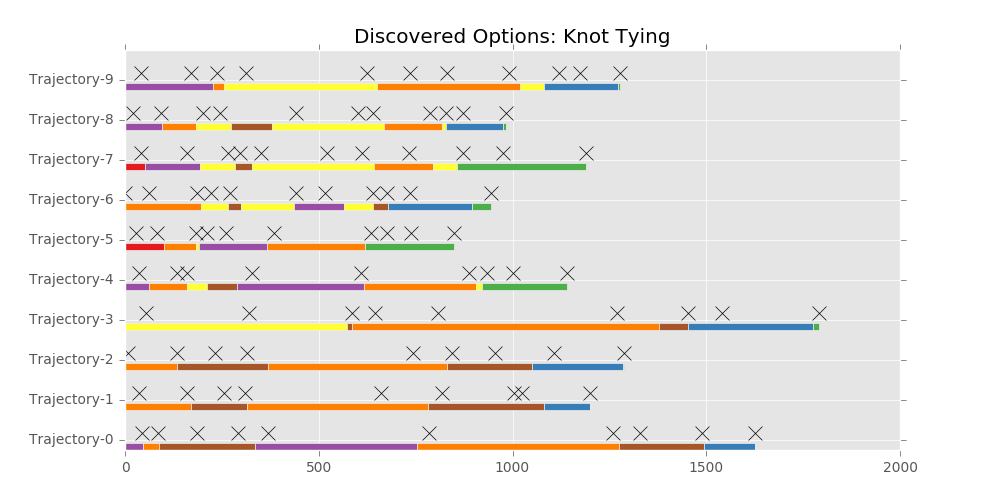
\includegraphics[width=0.7\columnwidth]{ddco-experiments/options-knot-tying.png}
    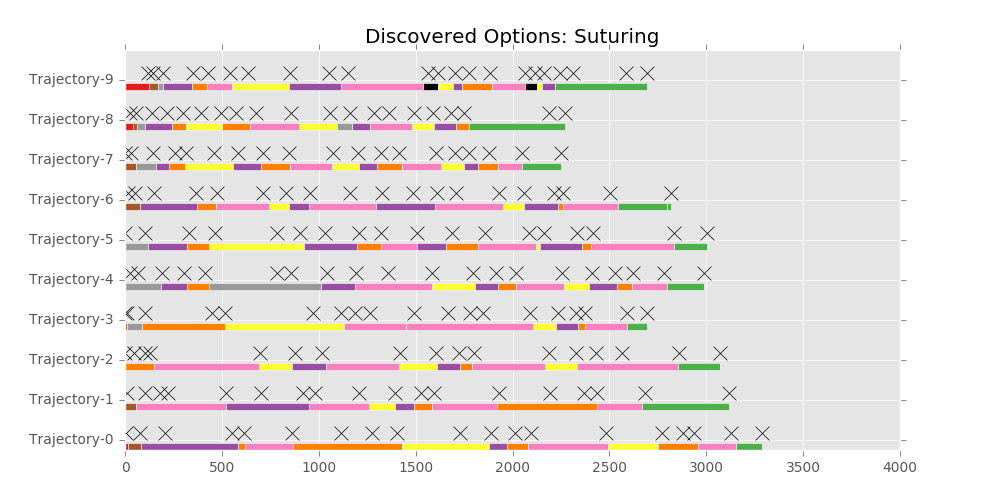
\includegraphics[width=0.7\columnwidth]{ddco-experiments/options-suturing.png}
    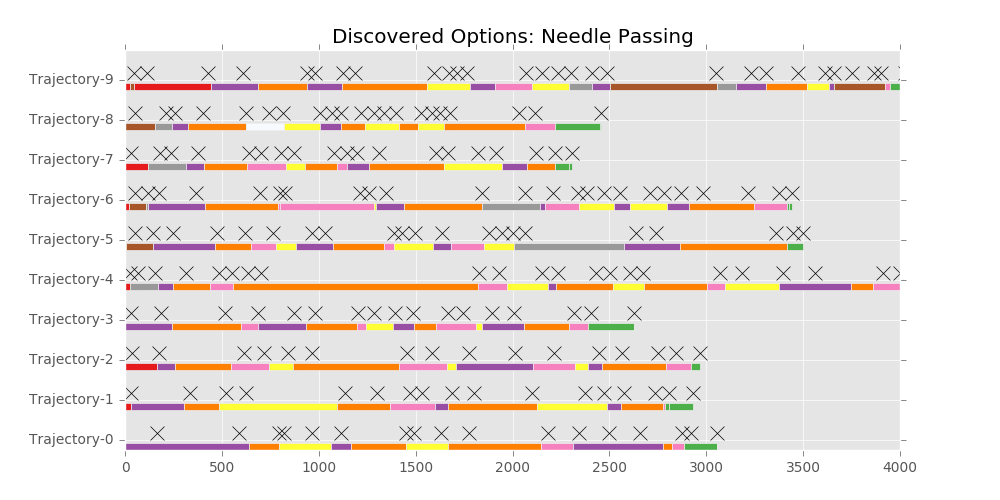
\includegraphics[width=0.7\columnwidth]{ddco-experiments/options-needle-passing.png}
    \caption{Segmentation of human demonstrations in three surgical tasks. Each line represents a trajectory, with segment color indicating the option inferred by \alg as most likely to be active at that time. Human annotations are marked as $\times$ above the segments. Automated segmentation achieves a good alignment with human annotation --- 72\% of option boundaries have exactly one annotation in a 300 ms window around them. \label{surgery-1}}
\end{figure}

\section{Experiments: Reinforcement}
We present an empirical study of \alg in the Reinforcement Learning setting. Our results suggest that \alg can discover options that accelerates reinforcement learning.

\subsection*{Four Rooms GridWorld \label{exp:gw-four-rooms}}
We study a simple four-room domain~(Figure~\ref{gw-1}). On a $15\times11$ grid, the agent can move in four directions; moving into a wall has no effect. To simulate environment noise, we replace the agent's action with a random one with probability $0.3$. An observable apple is spawned in a random location in one of the rooms. Upon taking the apple, the agent gets a unit reward and the apple is re-spawned.

We use the following notation to describe the different ways we can parametrize option discovery: \textsf{A} a baseline of only using atomic actions; \textsf{H1u} discovering a single level of options where the higher-level is parametrized by a uniform distribution; \textsf{H1s} discovering a single level of options where the higher-level is parametrized by an multi-layer perceptron (MLP); \textsf{H2u} and \textsf{H2s} are the two-level counterparts of \textsf{H1u} and \textsf{H1s}, respectively. All of these discovered options are used in an RL phase to augment the action space of a high-level global policy.

\begin{figure}[ht!]
    \centering
    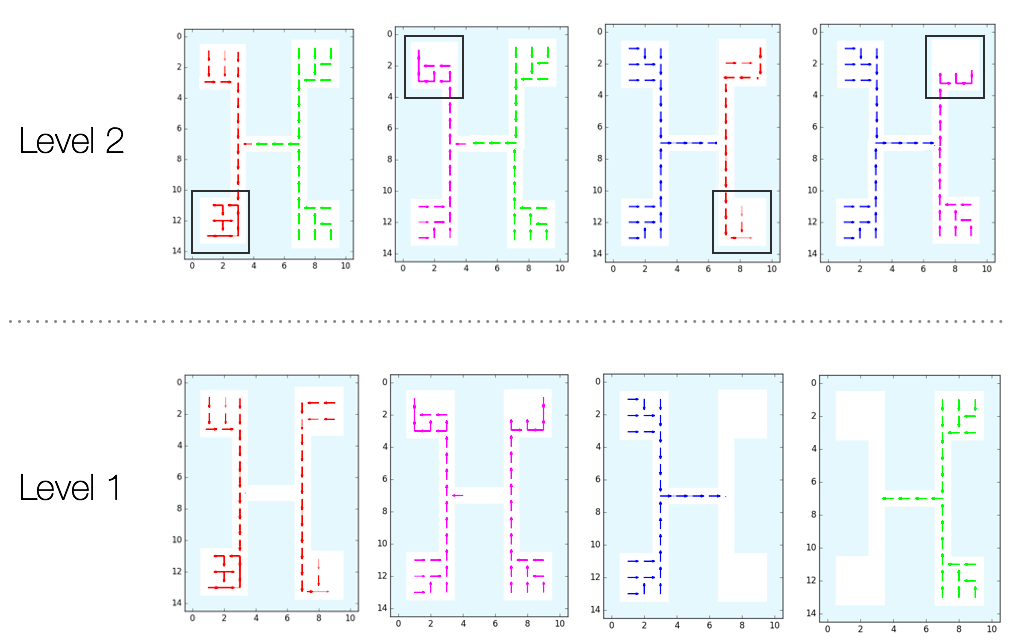
\includegraphics[width=\columnwidth]{ddco-experiments/ddo-4-rooms-results.png}
    \caption{Trajectories generated by options in a hierarchy discovered by \alg. Each level has 4 options, where level 2 builds on the level 1, which in turn uses atomic actions. In the lower level, two of the options move the agent between the upper and lower rooms, while the other two options move it from one side to the other. 
    In the higher level, each option takes the agent to a specific room. The lower-level options are color-coded to show how they are composed into the higher-level options. \label{gw-1}} 
\end{figure}

\begin{figure}[ht!]
    \centering
    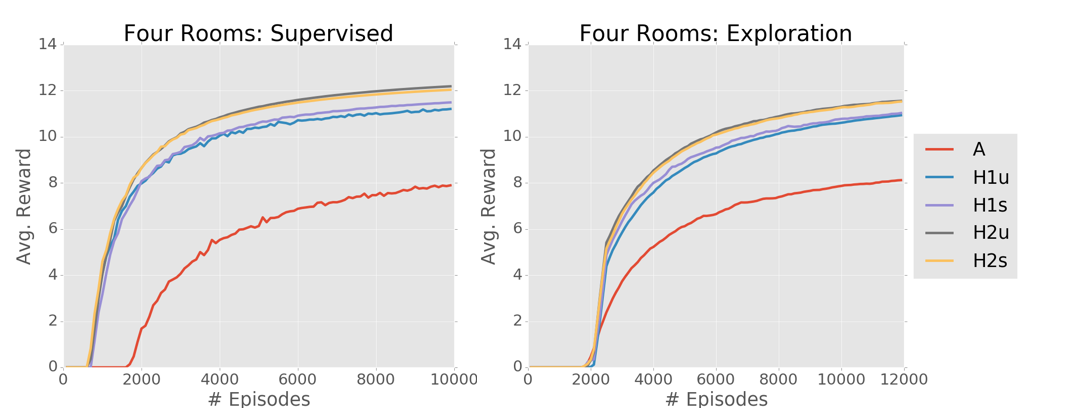
\includegraphics[width=\columnwidth]{ddco-experiments/4-rooms-clean.png}
    \caption{$15$-trial mean reward for the Supervised and Exploration problem settings when running DQN with no options (\textsf{A}), low-level options (\textsf{H1u}) and lower- and higher-level options (\textsf{H2u}) augmenting the action space. The options discovered by \alg can accelerate learning, since they benefit from not being interrupted by random exploration.  \label{gw-2}}
\end{figure}

{\bf Baseline.} We use Value Iteration to compute the optimal policy, and then use this policy as a supervisor to generate 50 trajectories of length 1000. All policies, whether for control, meta-control or termination, are parametrized by a MLP, with a single two-node hidden layer, and $\tanh$ activation functions. The MLP's input consists of the full state (agent and apple locations), and the output is computed by a $\mathrm{softmax}$ function over the MLP output vector, which has length $|\C A|$ for control policies and two for termination.

The options corresponding to \textsf{H2u} are visualized in Figure~\ref{gw-1} by trajectories generated using each option from a random initial state until termination. At the first level, two of the discovered options move the agent between the upper and lower rooms, and two move it from one side to the other. At the second level, the discovered options aggregate these primitives into higher-level behaviors that move the agent from any initial location to a specific room.

{\bf Impact of options and hierarchy depth.} To evaluate the quality of the discovered options, we train a Deep Q-Network (DQN) with the same MLP architecture, and action space augmented by the options. The exploration is $\epsilon$-greedy with $\epsilon=0.2$ and the discount factor is $\gamma=0.9$. Figure~\ref{gw-2} shows the average reward in $15$ of the algorithm's runs in the Supervised and Exploration experimental settings.
The results illustrate that augmenting the action space with options can significantly accelerate learning. Note that the  options learned with a two-level hierarchy (\textsf{H2u}) provide significant benefits over the options learned only with a single-level hierarchy \textsf{H1u}.
The hierarchical approaches achieve roughly the same average reward after 1000 episodes as \textsf{A} does after 5000 episodes.

{\bf Impact of policy parametrization.} To evaluate the effect of meta-control policy parametrization, we also compare the rewards during DQN reinforcement learning with options discovered with MLP meta-control policies (\textsf{H1s} and \textsf{H2s}). Our empirical results suggest that less expressive parametrization of the meta-control policy does not significantly hurt the performance, and in some cases can even provide a benefit (Figure \ref{gw-2}). This is highly important, because the high sample complexity of jointly training all levels of a deep hierarchy necessitates simplifying the meta-control policy --- which would otherwise be represented by a one level shallower hierarchy. We conjecture that the reason for the improved performance of the less expressive model is that more complex parametrization of the meta-control policy increases the prevalence of local optima in the inference problem, which may lead to worse options.

{\bf Exploration Setting.} Finally, we demonstrate that options can also be useful when discovered from self-demonstrations by a partially trained agent, rather than by an expert supervisor. We run the same DQN as above, with only atomic actions, for 2000 episodes. We then use the greedy policy for the learned $Q$-function to generate 100 trajectories.  We reset the $Q$-function (except for the baseline \textsf{A}), and run DQN again with the augmented action space. Figure \ref{gw-2} illustrates that even when these options are not discovered from demonstrations of optimal behavior, they are useful in accelerating reinforcement learning.
The reason is that options are policy fragments that have been discovered to lead to interesting states, and therefore benefit from not being interrupted by random exploration. 

%\ion{This paragraph is confusing. Not sure what does "30\% probability of random action" exactly mean. Not sure where the 11 goals are coming from.}In the first scenario, we construct a 15x10 GridWorld environment with four rooms with a 30\% probability of random action. Goal states are randomly drawn in each room and the agent has accumulate as many goals as possible in 1000 timesteps or a maximum of 11 total goals (each goal results in a reward of 1). We generate 50 demonstrations using Value Iteration. 

%\vspace{0.25em} \noindent \textbf{Model Parameterization: } The agent's state is a 4-dimensional vector $(x,y, g_x, g_y)$ where $(g_x,g_y)$ is the current goal. \ion{What does {\bf current} goal mean?} For this experiment, each  low-level option is a multi-layer perceptron (MLP) with a single hidden layer consisting of $2$ nodes that employ $\textsf{tanh}$ activation functions. The high-level meta-policy is parameterized by an i.i.d  uniform distribution. One of our hypotheses is that in the option discovery phase simple high-level policies suffice, as these policies will ultimately be re-learned on the transfer instance.

%\vspace{0.25em} \noindent \textbf{Learned Hierarchy: } We apply \alg to learn a two-level hierarchy where each level has four options (Figure \ref{gw-1}). The visualization shows trajectories sampled from the inferred options, i.e., start at a random state and apply the option until termination. Out of the four options we discover at the low level, two move the agent from the upper two rooms to the lower two rooms, and two move the agent from one side to the other. By adding a second level to the hierarchy \Roy{so this is L2+L3 after L1+U?}, we get higher level behaviors by aggregating the low-level options. In particular, the options we discover at the second level move an agent to a {\em particular} room starting from a random location.

%\vspace{0.25em} \noindent \textbf{Evaluating the Options: } Consider a new task instance where goal states are randomly sampled. Next, we evaluate whether (and how much) the options we learned in the two-level hierarchy improve the convergence of an RL algorithm. We use a Deep Q Network (DQN) as the RL algorithm. The Q-Network uses the same architecture as the options, i.e., a single-hidden layer MLP with two hidden nodes. We train the network with an $\epsilon$-greedy policy with discount factor of $\gamma=0.9$, and $\epsilon=0.2$, respectively.
%We compare three approaches: (1) DQN using only primitive actions, (2) DQN using the low-level options, in additions to all primitive actions, and (3) DQN using the options at both levels of the hierarchy, as well as all primitive actions.
%Figure \ref{gw-2} shows the average reward for each approach versus the number of episodes. These results clearly illustrate that augmenting the action space with options can significantly improve the convergence. There are two points worth noting. First, approach 3 (i.e., leveraging all options and primitive actions) achieves the same average reward as approach 1, 5x faster. Indeed, after less than $1000$ episodes, approach 3 achieves roughly the same average reward as approach 1 after $5000$ episodes. Second, the deeper hierarchy provides significant benefits over the single-level hierarchy. This is because options allow the agent to receive a reward faster.



%\vspace{0.25em} \noindent \textbf{Evaluating the Parameterization: } Next, we evaluate different parameterization strategies for the \alg. In particular, we consider the impact of the high-level meta policy's parameterization during the learning stag. In particular, we consider the following variants of the two-level hierarchy described before: (\textsf{L0}) No options, (\textsf{L1u}) single level of options with a uniform meta policy, (\textsf{L2u}) two levels of options both learned with uniform meta policies, (\textsf{L1s}) a single level of options learned with a state-dependent MLP meta policy, and (\textsf{L2s}) two levels of options both learned with state-dependent MLP meta policies. Using a uniform meta policy during the inference stage significantly reduces the number of parameters for learning, and our experimental results suggest that such a parameterization does not significantly hurt the performance (Figure \ref{gw-3}). In fact, results suggest that in some cases, the additional parameters can actually hurt. We conjecture this is because the more complex parameterization of the meta policies increases the number of local minima in the inference problem, which ultimately leads to some lower quality options.

%The decoupling between the low-level options and the high-level meta-policy is interesting because it facilitates scaling the hierarchy. If each level is decoupled from the previous one, it is easy to scale the number of levels in the hierarchy. Furthermore, the reduced parameterization improves learning performance (i.e., requires fewer demonstrations). However, we must caution that this is not a definitive result and warrants further investigating, which we plan to do in future work. There are clearly situations where using a more complex parameterization of the high-level policy can help differentiate between equally likely option assignments. Nonetheless, next, we leverage these preliminary results as a motivation for using a simplified high-level structure during the option discovery phase. 


%\subsection{GridWorld: Incremental}
%The previous scenario illustrates how options can facilitate transfer between task instances. Next, we show how within a task options can be used to improve the convergence of an RL algorithm by incrementally constructing options.
%We use the same four-room GridWorld as before.
%We use a Deep Q Network (DQN) as the RL algorithm.
%The Q-Network is constructed with the same basic architecture as the options (single-hidden layer MLP, 2 hidden nodes), and we train the network with an $\epsilon$-greedy policy with discount factor of $\gamma=0.9$ and $\epsilon=0.2$.
%We run the DQN over the original primitive action space for $2000$ episodes, then sample $100$ demonstrations from the current best policy, and then apply \alg. The future $13000$ episodes of the DQN are run with an augmented action space.
%This DQN is re-initialized and trained from scratch. 
%Figure \ref{gw-4} illustrates that even when these options are not derived from an optimal supervisor, they are useful in improving the long term performance of the agent.
%This is because that the agent is allowed to reuse previously learned behaviors without having to re-learn them through exploration.


\subsection*{Atari RAM Games}
The RAM variant of the popular Atari Deep Reinforcement Learning domains considers a game-playing agent which is given not the screen, but rather the RAM state of the Atari machine.
This RAM state is a 128-byte vector that completely determines the state of the game, and can be encoded in one-hot representation as $s\in\F R^{128 \times 256}$.
The RAM state-space illustrates the power of an automated option discovery framework, as it would be infeasible to manually code options without carefully understanding the game's memory structure.
With a discovery algorithm, we have a general-purpose approach to learn in this environment.

All policies are parametrized with a deep network. There are three dense layers, each with $\tanh$ activations, and the output distribution is a $\mathrm{softmax}$ of the last layer, which has length $|\C A|$ for control policies and two for termination. We use a single level of options, with the number of options tuned to optimize performance, and given in Figure~\ref{atari-1}.

For each game, we first run the DQN for $1000$ episodes, and then generate $100$ trajectories from the greedy policy, and use them to discover options with \alg.
The DQN has the same architecture, using $\epsilon$-greedy exploration for $1000$ episodes with $\epsilon=0.05$ and discount factor $\gamma=0.85$ (similar to the parameters used in~\citep{sygnowski2016learning}). 
Finally, we augment the action space with the discovered options and rerun DQN for $4000$ episodes. 
We compare this to the baseline of running DQN for $5000$ episodes with actions only.

Figure \ref{atari-1} plots the estimate value, averaged over $50$ trials, of the learned policies for five Atari games: Atlantis, Pooyan, Gopher, Space Invaders, and Sea Quest.
In four out of five games, we see a significant acceleration learning.
The relative improvements are the largest for the three hardest domains: Gopher, Sea Quest, and Space Invaders.
It is promising that \alg offers such an advantage where other methods struggle. 
Figure \ref{atari-3} shows four frames from one of the options discovered by \alg for the Atlantis game. %\footnote{In the final version, we will provide a link to the videos of the learned options.}.
The option appears to identify an incoming alien and determine when to fire the gun, terminating when the alien is destroyed.
As in the GridWorld experiments, the options are policy fragments that have been discovered to lead to high-value states, and therefore benefit from not being interrupted by random exploration.

\begin{figure}[ht!]
    \centering
    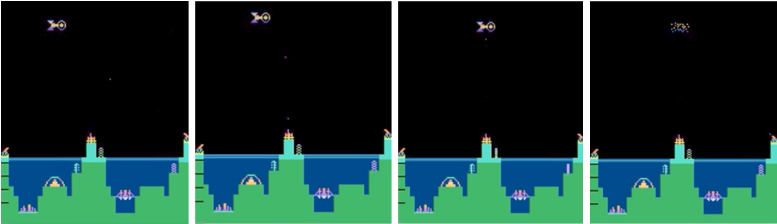
\includegraphics[width=\columnwidth]{ddco-experiments/atlantis-primitive.png}
    \caption{Frames sampled from a demonstration trajectory assigned to one of the primitives learned from \alg.  \label{atari-3}}
\end{figure}


\begin{figure}[ht!]
    \centering
    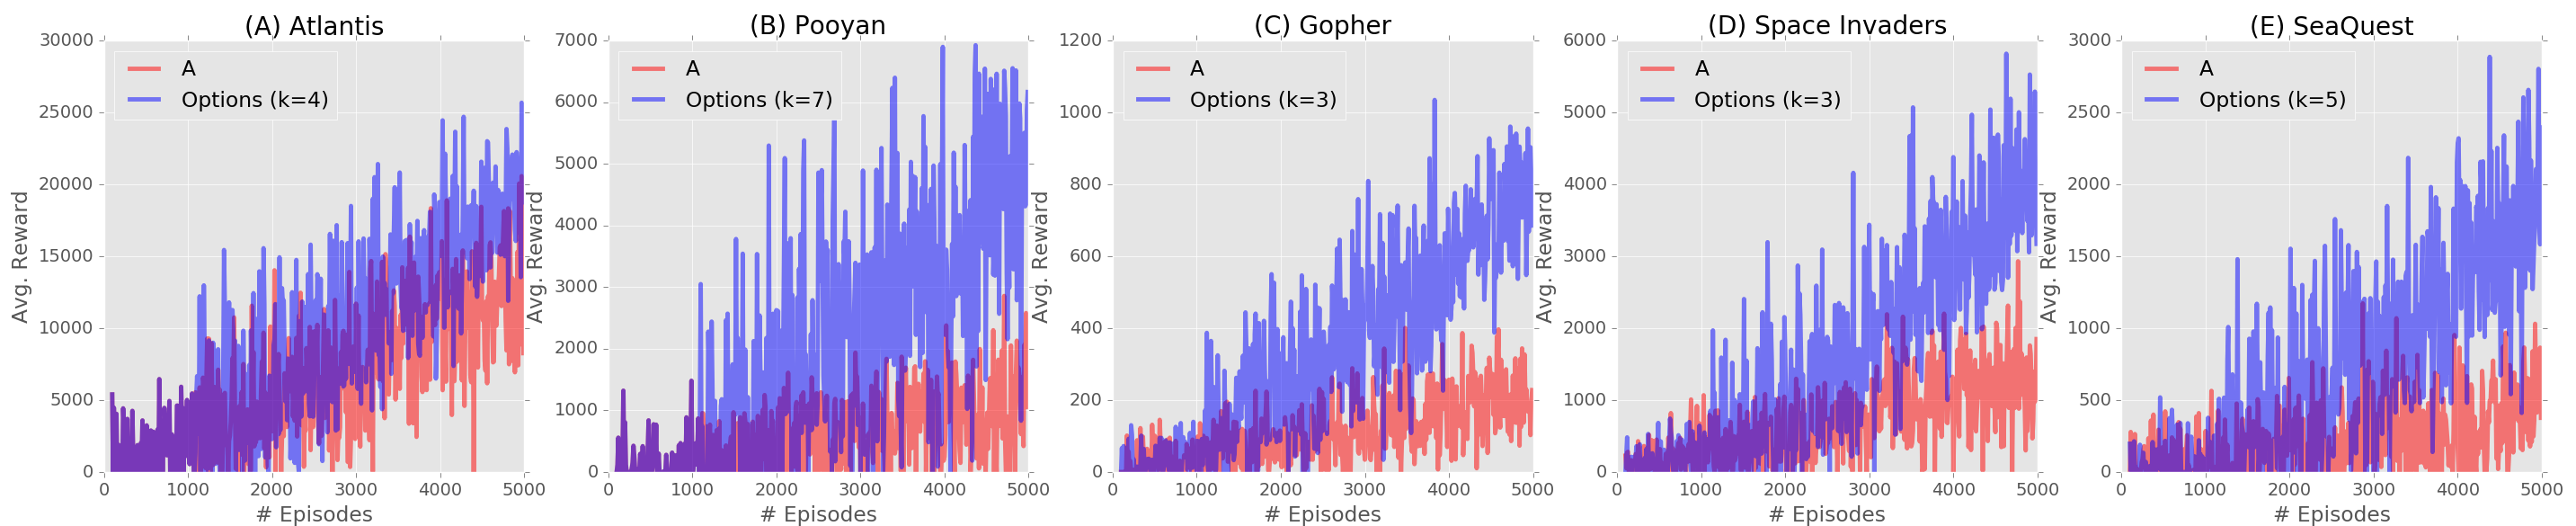
\includegraphics[width=\textwidth]{ddco-experiments/exp5-atari.png}
    \caption{Atari RAM Games: Average reward computed from 50 rollouts when running DQN with atomic actions for 1000 episodes, then generating 100 trajectories from greedy policy, from which \alg discovers options in a 2-level hierarchy. DQN is restarted with action space augmented by these options, which accelerates learning in comparison to running DQN with atomic actions for 5000 episodes. Results suggest significant improvements in 4 out of 5 domains. \label{atari-1}}
\end{figure}


\chapter{Sequential Windowed Inverse Reinforcement Learning: Learning Reward Decomposition From Data}
\chaptermark{SWIRL}
In the previous chapter, I considered a model where sequences of state-action tuples from an expert demonstrator were available.
Next, we consider a setting where only the state sequence is observed.
This can happen when the demonstration modality differs from the execution setting, e.g., learning from third person videos, motion capture of a human doing a task, or kinesthetic demonstrations. 
Thus, the data cannot be directly used to derive a controller since the actions are not visible.
So, we approach this problem with a simple premise;  \emph{change in reward function implies change in behavior}.
Like DDO, we apply unsupervised learning to a small number of initial expert demonstrations to learn a latent reward structure. This requires two pieces: robustly detecting consistent changes in state trajectories and constructing reward functions around those change points.

As a motivating example from the problem setting consider the widespread adoption of robot-assisted minimally invasive surgery (RMIS), which is generating datasets of kinematic and video recordings of surgical procedures~\cite{gao2014jigsaws}.
Explicitly modeling the system dynamics can require learning a large number of parameters.
This makes a direct system identification approach somewhat sensitive to any noise in the dataset, especially when the datasets are small. 
Furthermore, the states are often high-dimensional with combinations of kinematic and visual features.

Suppose, one could decompose a surgical task into a consistent sequence of sub-tasks.
While each demonstration motion may vary and be noisy, each demonstration also contains roughly the same order of true segments.
This consistent, repeated structure can be exploited to infer global segmentation criteria.
By assuming known sequential segment-to-segment ordering, the problem reduces to identifying a common set of segment-to-segment transition events--not corresponding entire the trajectory segments across the whole dataset.
This allows us to apply coarser, imperfect motion-based segmentation algorithms first that create a large set of candidate transitions.
Then, we can filter this set by identifying transition events that occurred at similar times and states.
Our experiments suggest that this approach has improved robustness and sample-efficiency, while approximating the behavior of more complicated dynamical systems-based approaches in many real problems.

I formalize this intuition into a new hierarchical clustering algorithm for unsupervised segmentation called Transition State Clustering.
The proposed approach is also relevant to problems in other domains, but I will focus on results from surgical applications.
\tsc first applies a motion-based segmentation model over the noisy trajectories and identifies a set of candidate segment transitions in each.
\tsc then clusters the transition states (states at times transitions occur) in terms of kinematic, sensory, and temporal similarity. 
The clustering process is hierarchical where the transition states are first assigned to Gaussian Mixture clusters according to kinematic state, then these clusters are sub-divided using the sensory features, and finally by time.
We present experiments where these sensory features are constructed from video.
The learned clustering model can be applied to segment previously unseen trajectories by the same global criteria.
To avoid setting the number of clusters at each level of the hierarchy in advance, the number of regions are determined by a Dirichlet Process prior.
A series of merging and pruning steps remove sparse clusters and repetitive loops.


\section{Transition State Clustering}
This section describes the problem setting, assumptions, and notation.
Let $D=\{d_i\}$ be a set of demonstrations of a robotic task.
Each demonstration of a task $d$ is a discrete-time sequence of $T$ state vectors in a feature-space $\mathcal{X}$.
The feature space is a concatenation of kinematic features $X$ (e.g., robot position) and sensory features $V$ (e.g., visual features from the environment).

\begin{definition}[Segmentation]
A segmentation of a task is defined as a function $\mathbf{S}$ that assigns each state in every demonstration trajectory to an integer $1,2,...,k$:
\[
\mathcal{S}: d \mapsto (a_n)_{1,...,|d|}, a_n \in {1,...,k}.
\]
and $\mathcal{S}$ is a non-decreasing function in time (no repetitions).
\end{definition}

Suppose we are given a function that just identifies candidate segment endpoints based on the kinematic features.
Such a function is weaker than a segmentation function since it does not globally label the detected segments.
This leads to the following definition:

\begin{definition}[Transition Indicator Function]
A transition indicator function $\mathbf{T}$ is a function that maps each kinematic state in a demonstration $d$ to $\{0,1\}$:
\[
\mathbf{T}: d \mapsto (a_n)_{1,...,|d|}, a_n \in {0,1}.
\]
\end{definition}

The above definition naturally leads to a notion of transition states, the states and times at which transitions occur.

\begin{definition}[Transition States]
For a demonstration $d_i$, let $o_{i,t}$ denote the kinematic state, visual state, and time $(x,v,t)$ at time $t$.
Transition States are the set of state-time tuples where the indicator is 1:
\[
\Gamma = \bigcup_{i}^N ~\{o_{i,t} \in d_i ~: \mathbf{T}(d_i)_t = 1\}.
\]
\end{definition}

The goal of \tsc is to take the transition states $\Gamma$ and recover a segmentation function $\mathbf{S}$. This segmentation function is stronger than the provided $\mathbf{T}$ since it not only indicates that a transition has occurred but labels the segment transition consistently across demonstrations.

\subsection*{Assumptions}
We assume that all possible true segments are represented in each demonstration by at least one transition (some might be false positives).
Given the segmentation function $\mathcal{S}(d_i)$, one can define a set of \emph{true} transition states:
\[\Gamma^* = \{
o_{i,t} \in d_i : ~\mathcal{S}(d_i)_{t-1} \ne \mathcal{S}(d_i)_t,~ t > 0\}.
\]
These satisfy the following property:
\[
 \Gamma^* \subseteq \Gamma.
\]
In other words, we assume that a subset of transition states discovered by the indicator function correspond with the true segment transitions.
There can be false positives but no false negatives (a demonstration where a segment transition is missed by the transition indicator function).
Since the segmentation function is sequential and in a fixed order, this leads to a model where we are trying to find the $k-1$ true segment-segment transition points in $\Gamma$.

\subsection*{Problem Statement and Method Overview}\label{ps}
These definitions allow us to formalize the transition state clustering problem. 

\begin{problem}[Transition State Clustering]
Given a set of regular demonstrations $D$ and transition identification function $\mathbf{T}$, find a segmentation $\mathbf{S}$.
\end{problem}

\noindent \textbf{Candidate Transitions: } To implement $\mathbf{T}$, \tsc fits a Gaussian mixture model to sliding windows over each of the demonstration trajectories and identifies consecutive times with different most-likely mixture components.

\vspace{0.25em}

\noindent \textbf{Transition State Clusters: } The states at which those transitions occur are called transition states.
\tsc uses a GMM to cluster the transition states in terms of spatial and temporal similarity to find $\mathbf{S}$.

\vspace{0.25em}

\noindent \textbf{Optimizations: } To avoid setting the number of clusters at each level of the hierarchy in advance, the number of regions are determined by a Dirichlet Process prior.
A series of merging and pruning steps remove sparse clusters and repetitive loops.

\subsection*{Gaussian Mixture Transition Identification}
While we can use any transition identification function to get $\Gamma$ (as long as it satisfies the assumptions), we present one implementation based of Gaussian Mixtures that we used in a number of our experiments.
We found that this GMM approach was scalable (in terms of data and dimensionality) and had fewer hyper-parameters to tune than more complex models.
Combined with the subsequent hierarchical clustering, this approach proved to be robust in all of our experiments.

\begin{algorithm}[t]
\caption{Transition Identification \label{ialgotext}}
\begin{algorithmic}[1]
\State \textsf{Input: } $D$ demonstrations, $\ell$ a window size, and $\alpha$ a Dirichlet Process prior.

\State For each demonstration, generate a set of sliding windows of $\mathbf{w}^{(\ell)}_t = [\mathbf{x}_{t-\ell},...,\mathbf{x}_{t}]^\intercal$. Let $W$ be the set of all sliding windows across all demonstrations.

\State Fit a mixture model to $W$ assigning each state to its most likely component. 

\State Identify times $t$ in each demonstration when $\mathbf{w}_t$ has a different most likely mixture component than $\mathbf{w}_{t+1}$, start and finish times ($t=0,t=T_i$) are automatically transitions. 

\State \textsf{Return: } A set of transition states $\Gamma$, the $(x,v, t)$ tuples at which transitions occur.

\end{algorithmic}

\end{algorithm}

Each demonstration trajectory $d_i$ is a trajectory of $T_i$ state-vectors $[x_1,...,x_{T_i}]$.
For a given time $t$, we can define a window of length $\ell$ as:
\[
\mathbf{w}^{(\ell)}_t = [s_{t-\ell},...,s_{t}]^\intercal
\]
We can further normalize this window relative to its first state:
\[
\mathbf{n}^{(\ell)}_t = [s_{t-\ell}-s_{t-\ell},...,s_{t}-s_{t-\ell}]^\intercal
\]
This represents the ``delta'' in movement over the time span of a window.
Then, for each demonstration trajectory we can also generate a trajectory of $T - \ell$ windowed states:
\[
\mathbf{d}^{(\ell)} = [\mathbf{n}^{(\ell)}_\ell,...,\mathbf{n}^{(\ell)}_{T}]
\]
Over the entire set of windowed demonstrations, we collect a dataset of all of the $\mathbf{n}^{(\ell)}_t$ vectors.
We fit a GMM model to these vectors.
The GMM model defines $m$ multivariate Gaussian distributions and a probability that each observation $\mathbf{n}^{(\ell)}_t$ is sampled from each of the $m$ distributions.
We annotate each observation with the most likely mixture component.
Times such that $\mathbf{n}^{(\ell)}_t$ and $\mathbf{n}^{(\ell)}_{t+1}$ have different most likely components are marked as transitions.
This model captures some dynamical behaviors while not requiring explicit modeling of the state-to-state transition function.

Sometimes the MDP's states are more abstract and do not map to space where the normalized windows make sense.
We can still apply the same method when we only have a positive definite kernel function over all pairs of states $\mathbf{\kappa}(s_i,s_j)$.
We can construct this kernel function for all of the states observed in the demonstrations and apply Kernelized PCA to the features before learning the transitions--a technique used in Computer Vision~\cite{DBLP:conf/nips/MikaSSMSR98}.
The top $p'$ eigenvalues define a new embedded feature vector for each $\omega$ in $\mathbb{R}^{p'}$.
We can now apply the algorithm above in this embedded feature space.


\subsection*{TSC Inference Algorithm}
We present the clustering algorithm which is summarized in Algorithm \ref{algotext}.
In a first pass, the transition states are clustered with respect to the kinematic states, then sub-clustered with respect to the sensory states, and then, we temporally sub-cluster.
The sub-clusters can be used to formulate the segmentation criteria.

\begin{algorithm}[t]
\caption{Transition State Clustering \label{algotext}}
\begin{algorithmic}
\State \textsf{Input: } $\Gamma$ Transition States, $\rho$ pruning parameter

\State Fit a mixture model to the set of transition states $\Gamma$ in the kinematic states.

\State Fit a mixture model to the sensory features for transitions within every kinematic cluster $i$.

\State Fit a mixture model to the times from every kinematic and sensory cluster pair $(i,j)$.

\State Remove clusters that contain fewer than transition states from fewer than $\rho \cdot N$ distinct demonstrations.

\State \textsf{Output: } A set of transitions, which are regions of the state-space and temporal intervals defined by Gaussian confidence intervals.

\end{algorithmic}

\end{algorithm}

\vspace{0.5em}\noindent\textbf{Kinematic Step: } We want our model to capture that transitions that occur in similar positions in the state-space across all demonstrations are actual transitions, and we would like to aggregate these transitions into logical events. 
Hypothetically, if we had infinite demonstrations $\Gamma$ would define a density of transition events throughout the state-space.
The modes of the density, which intuitively represent a propensity of a state $x$ to trigger a segment change, are of key interest to us. 

We can think of the set of identified transition states $\Gamma$ as a sample of this density.
We fit a DP-GMM to kinematic features of the transition states.
Each transition state will have an assignment probability to one of the mixture components.
We convert this to a hard assignment by assigning the transition state to the most likely component.

\vspace{0.5em}\noindent\textbf{Sensory Step: }
Then, we apply the second level of DP-GMM fitting over the sensory features (if available).
Within each kinematic cluster, we fit a DP-GMM to find sub-clusters in the sensory features.
Note that the transitions were only identified with kinematic features.
This step grounds the detected transitions in sensory clusters.

\vspace{0.5em}\noindent\textbf{Temporal Step: }Finally, we apply the last level of DP-GMM fitting over the time axis.
Without temporal localization, the transitions may be ambiguous.
For example, in a figure 8 motion, the robot may pass over a point twice in the same task.
Conditioned on the particular state-space cluster assignment, we can fit a DP-GMM each to each subset of times.
The final result contains sub-clusters that are indexed both in the state-space and in time.

\vspace{0.5em}\noindent\textbf{Enforcing Consistency: }
The learned clusters will vary in size as some may consist of transitions that appear only in a few demonstrations. The goal of \tsc is to identify those clusters that correspond to state and time transition conditions common to all demonstrations of a task.
We frame this as a pruning problem, where we want to enforce that all learned clusters contain transitions from a fraction of $\rho$ distinct demonstrations.
Clusters whose constituent transition states come from fewer than a fraction $\rho$ demonstrations are \emph{pruned}.
$\rho$ should be set based on the expected rarity of outliers.
For example, if $\rho$ is 100\% then the only mixture components that are found are those with at least one transition state from every demonstration (i.e., the regularity assumption).
If $\rho$ is less than 100\%, then it means that every mixture component must cover some subset of the demonstrations.
In our experiments, we set the parameter $\rho$ to 80\% and show the results with and without this step.

\vspace{0.5em}\noindent\textbf{Segmentation Criteria: }
Finally, if there are $k$ remaining clusters $\{C_1,...,C_k\}$, we can use these clusters to form a criteria for segmentation. 
Each cluster is formed using a GMM triplet in the kinematic state, visual state, and time.
The quantiles of the three GMMs will define an ordered sequence of regions $[\rho_1,...,\rho_k]$ over the state-space and each of these regions has an associated time interval defined by the Gaussian confidence interval for some confidence level $z_{\alpha}$.


\subsection{TSC Simulated Experimental Evaluation}
 We evaluate \tsc's robustness in the following way:
\begin{enumerate}
   \item \emph{Precision. } Results suggest \tsc significantly reduces the number of false positive segments in simulated examples with noise.
   \item \emph{Recall. } Among algorithms that use piecewise linear segment models, results suggest \tsc recovers segments of a generated piecewise linear trajectory more consistently in the presence of process and observation noise.
   \item \emph{Applicability to Real-World Data. } Result suggest that \tsc recovers qualitatively relevant segments in real surgical trajectory data.
\end{enumerate}

\subsubsection{Precision in Synthetic Examples}
Our first experiment evaluates the following hypothesis: \tsc significantly reduces the number of false positive segments in a simple simulated example with noise. These experiments evaluate \tsc against algorithms with a single level of clustering.

Comparison of 7 alternative segmentation criteria:
\begin{enumerate}
    \item \emph{Zero-Velocity Crossing (VEL): } This algorithm detects a change in the sign of the velocity. 
    \item \emph{Smoothed Zero-Velocity Crossing (VELS): } This algorithm applies a low-pass filter (exponentially weighted moving average) to the trajectory, and then detects a change in the sign of the velocity.
    \item \emph{Acceleration (ACC): } This algorithm detects any change in the velocity by looking for non-zero acceleration.
    \item \emph{Gaussian Mixture Model (GMM): } This algorithm applies a GMM model to the observed states and detects changes in most likely assignment. The number of clusters were set to 2.
    \item \emph{Windowed Gaussian Mixture Model (GMMW): } This algorithm is the first phase of \tsc. It applies a GMM to windows of size 2, and detects changes in most likely assignment. The number of clusters was set to 2, unlike in \tsc where we use the DP to set the number of clusters.
    \item \emph{Auto-Regressive Mixture (AR): } This model fits a piecewise linear transition law to the observed data.
    \item  \emph{Coresets (CORE): } We evaluate against a standard coreset model~\cite{sung2012trajectory, volkov2015coresets}, and the particular variant is implemented with weighted k-means. We applied this to the same augmented state-vector as in the previously mentioned GMM.
    \item \emph{\tsc: } Our proposed approach with a pruning threshold of $0.8$ and no loop compaction.
\end{enumerate}

\begin{figure}[ht!]%[t]
\centering
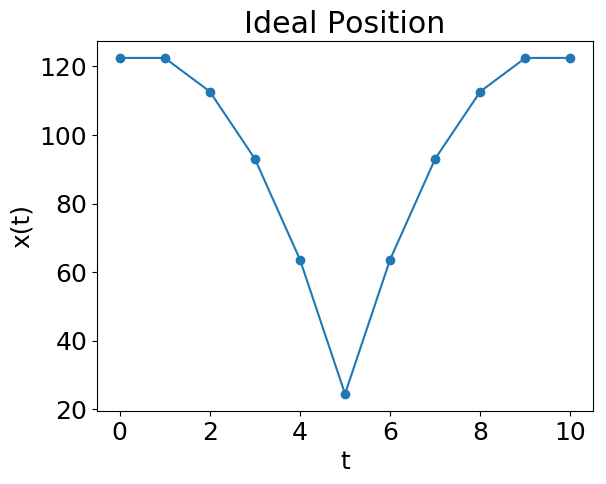
\includegraphics[width=0.48\columnwidth]{tsc-experiments/a.png}
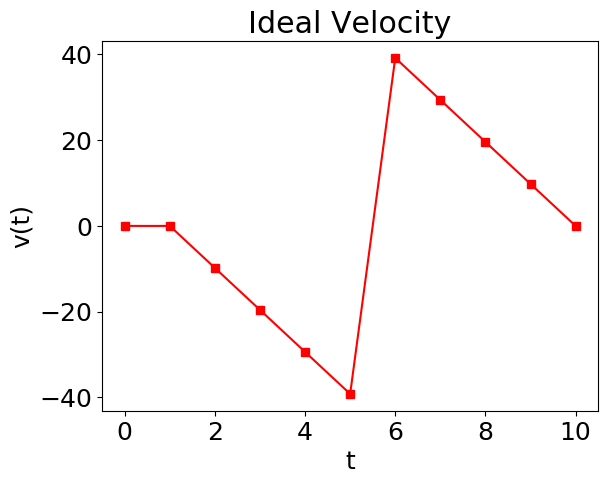
\includegraphics[width=0.48\columnwidth]{tsc-experiments/b.png}
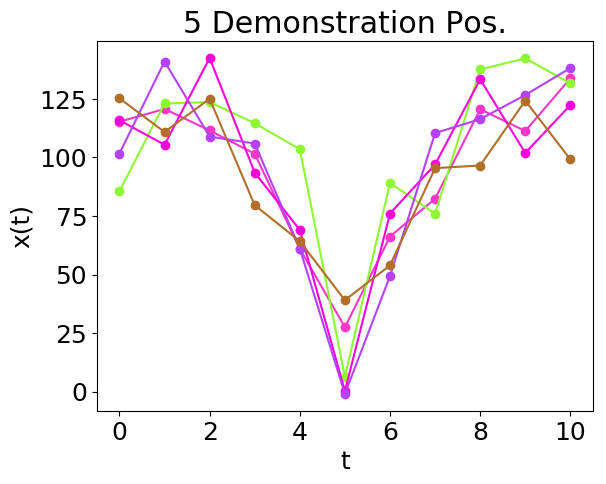
\includegraphics[width=0.48\columnwidth]{tsc-experiments/c.png}
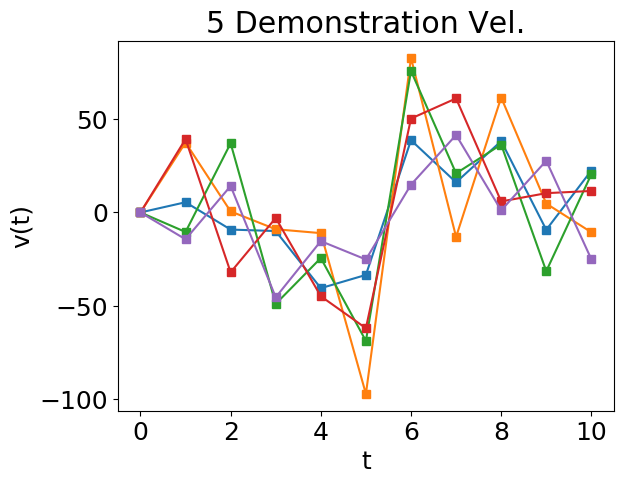
\includegraphics[width=0.48\columnwidth]{tsc-experiments/d.png}
\caption{(Above) The position and velocity of the bouncing ball without noise. (Below) 5 trajectories of the ball with different realizations of the noise. \label{ball-diagram}}
% \vspace{-1em}
\end{figure}

\begin{figure}[ht!]
\centering
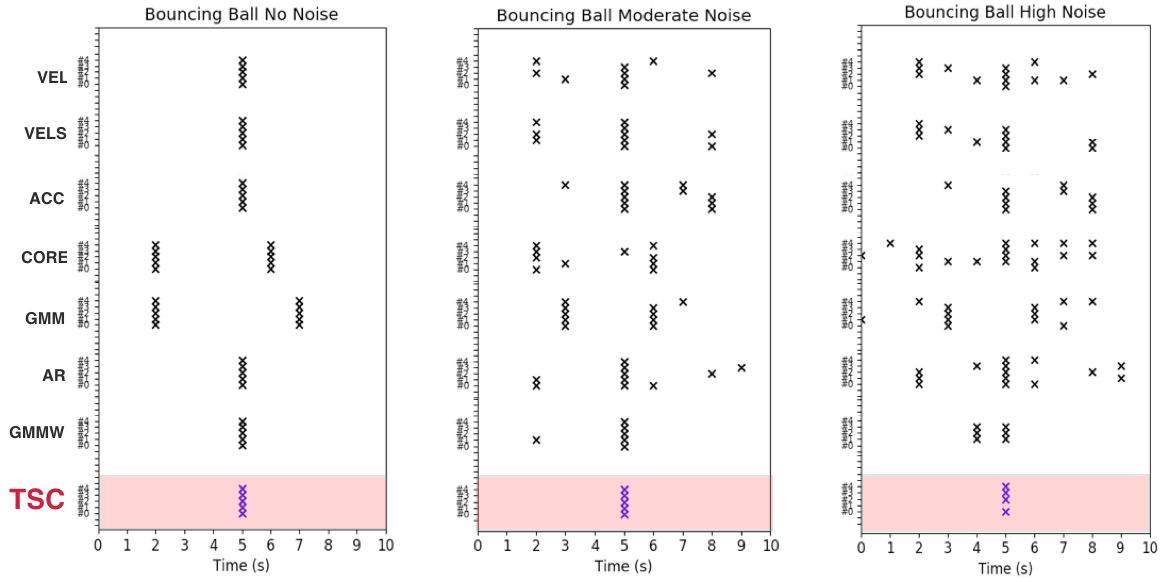
\includegraphics[width=\columnwidth]{tsc-experiments/ball-results.png}
\caption{Plots the identified transitions with each segmentation algorithm with and without noise. While all techniques are precise when there is no noise, \tsc is the most robust in the presence of noise. \label{ball-results}}
% \vspace{-1em}
\end{figure}


\textbf{Bouncing Ball: }
We first revisit the example in the introduction of the bouncing ball, which can be modeled as the following 1D double-integrator system:
\[ \ddot{x} = \unitfrac[-9.8]{\metre}{\second^2} \]
This system is observed with additive Gaussian white noise with std. 10 (Moderate Noise):
\[
y = x + N(0,10)
\]
and std. 20 (High Noise):
\[
y = x + N(0,20)
\]
The system is initialized at $x_0 = 122.5$ and bounces when $x=20$, at which point the velocity is negated.
Figure \ref{ball-diagram} illustrates the ideal trajectory and noisy realizations of these trajectories.

We apply the segmentation algorithms to the trajectories and plot the results in Figure \ref{ball-results}.
When there is no noise, all of the algorithms are equally precise, and there is no trouble corresponding segments across demonstrations.
All of the ``rate-of-change'' methods (VEL, VELS, ACC) reliably identify the point where the ball bounces.
The GMM and the Coreset methods do not segment the trajectory at the bounce point. 
On the other hand, the windowed GMM takes two consecutive positions and velocities into account during the clustering.
Similarly, the autoregressive model can accurately identify the bounce point.
With no noise, \tsc has little difference with the windowed GMM.

Differences arise when we observe the trajectory with additive Gaussian noise.
The ``rate-of-change'' methods have some spurious segmentation points due to noise. 
The GMM based methods are more robust to this noise, and they retain similar precision.
This motivates our choice of the first phase of the \tsc algorithm using a windowed GMM approach.
However, the GMM approaches still have some spurious transitions.
With these spurious points, it becomes challenging to reliably correspond trajectories across segments.
So, \tsc applies a second phase of clustering to correspond the transitions and prune the sparse clusters.
This results in accurate segmentation even in the presence of noise.

As the noise increases, \tsc is still able to find accurate segments.
In the high noise case, the bounce point is still identified in 4 out of 5 trajectories.
It is important to note that we do not claim that one segmentation algorithm is more accurate than another, or that \tsc more accurately reflects ``real'' segments.
These results only suggest that \tsc is more precise than alternatives; that is, given the assumptions in \tsc it consistently recovers segments according to those assumptions.
The next experiments will study the recall characteristics.

\begin{figure}[ht!]%[t]
\centering
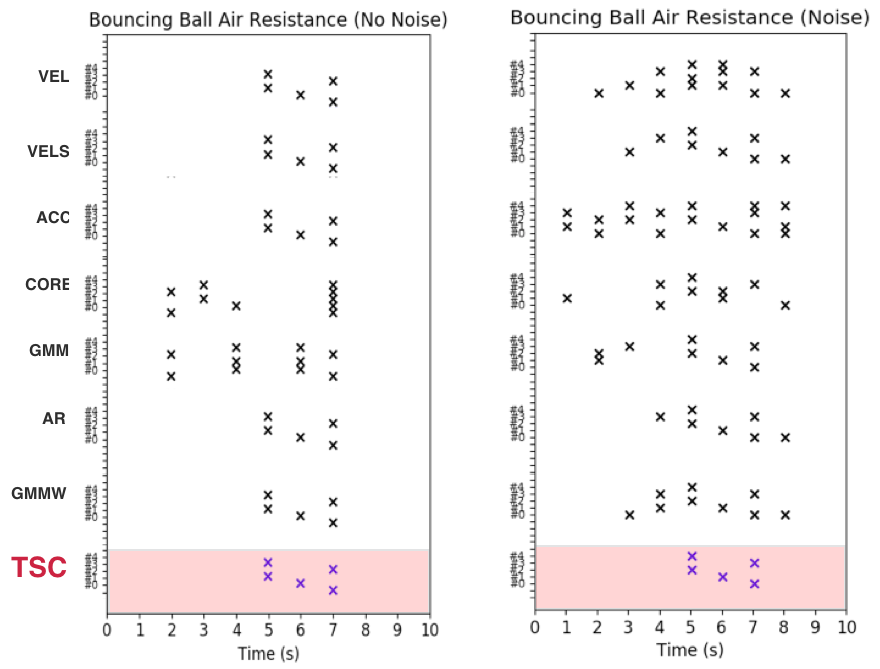
\includegraphics[width=\columnwidth]{tsc-experiments/ball-results2.png}
\caption{Plots the identified transitions with each segmentation algorithm with and without noise. In this example, temporal variation is added by incorporating a random ``air resistance'' factor.
\tsc is consistent even in the presence of this temporal variation. \label{ball-results2}}
% \vspace{-1em}
\end{figure}

\textbf{Bouncing Ball with Air Resistance: }
In the first set of experiments, we illustrate \tsc's robustness to variance in the state-space.
Next, we illustrate how \tsc can still correspond segments with temporal variation.
Consider the dynamics of the bouncing ball with an term to account for air resistance:
\[ \ddot{x} = \unitfrac[-9.8]{\metre}{\second^2} + K_v \dot{x} \]
We draw the air-resistance constant $K_v$ uniformly from $K_v \sim U[1,5]$.
The consequence is that that the ball will bounce at different times in different trajectories.

Figure \ref{ball-results2} illustrates the results.
In the 5 trajectories, the ball bounces between time-step 5 and 7.
With no noise VEL, VELS, ACC, GMMW, and \tsc can identify the bounce point.
Then, the system is observed with additive Gaussian white noise with std. 10:
\[
y = x + N(0,10)
\]
We find that \tsc recovers a consistent set of segments even with the temporal variation.

\begin{figure}[ht!]%[t]
\centering
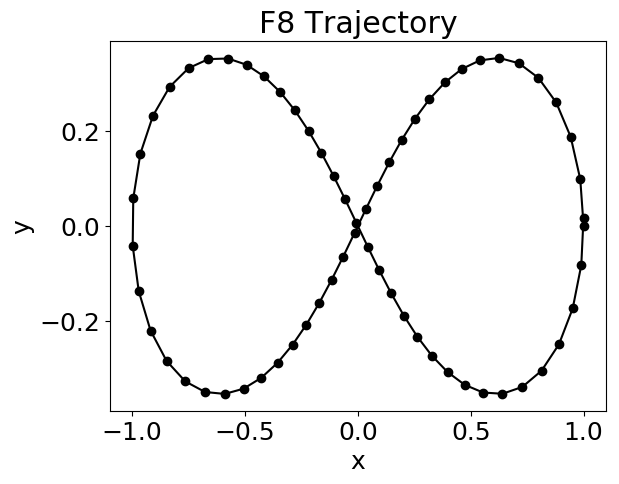
\includegraphics[width=0.48\columnwidth]{tsc-experiments/a1.png}
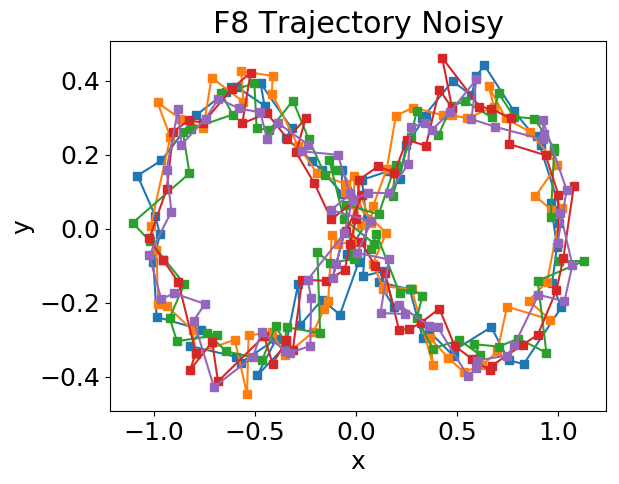
\includegraphics[width=0.48\columnwidth]{tsc-experiments/b1.png}
\caption{A ``figure 8'' trajectory in the plane, and 5 noisy demonstrations. The trajectory starts at the far right and progresses until it returns to the same spot. \label{f8-diagram}}
% \vspace{-1em}
\end{figure}

\begin{figure}[ht!]%[t]
\centering
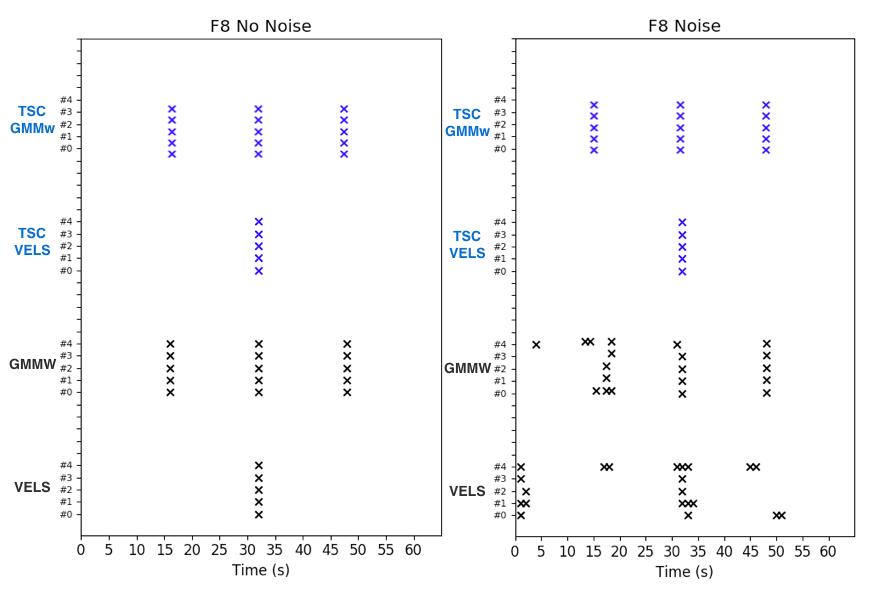
\includegraphics[width=\columnwidth]{tsc-experiments/hybrid_approach.png}
\caption{Plots the identified transitions with each segmentation algorithm with and without noise. Velocity based segmentation finds one transition point where there is a change in direction. A windowed GMM where the number of clusters is set by a DP finds three transition points. \tsc can improve the precision of both techniques.  \label{f8-results}}
% \vspace{-1em}
\end{figure}


\textbf{Hybrid Approaches: } In the previous experiments, we presented \tsc using a windowed GMM approach to identify transitions. Next, we consider \tsc with alternative transition identification functions.
Consider a ``Figure 8'' trajectory defined parametrically as:
\[
x = \textbf{cos}(t)
\]
\[
y = 0.5\textbf{sin}(2t)
\]
The trajectory is visualized in Figure \ref{f8-diagram}. The trajectory starts at the far right and progresses until it returns to the same spot. Velocity based segmentation finds one transition point where there is a change in direction (far left of the trajectory) (Figure \ref{f8-results}). 
A windowed GMM where the number of clusters is set by a DP finds three transition points. 
These three points correspond to the far left point as well as the crossing point in the figure 8 (happens twice).
These are two different segmentation criteria, and both are reasonable with respect to their respective assumptions.

Next, this parametric trajectory is observed with additive Gaussian noise of std. 0.1 (Figure \ref{f8-diagram}).
We see that both the GMM approach and the velocity approach have several spurious transitions (Figure \ref{f8-results}).
\tsc can improve the precision of both techniques by adding a layer of clustering.

\subsubsection{Rotations}
Handling orientations is a challenging problem due to the topology of $SO(3)$~\cite{ude2014orientation}. 
As an example of what can go wrong consider a 2D square rotating in the plane.
We construct a 1x1 meter 2D square and track a point on the corner of the 2D square.
The 2D square rotates clockwise in $\frac{\pi}{10}$ radian/s for 
10 time-steps, then switches, and rotates the other direction at the same angular speed.
The state of the system is the $(x,y)$ position of the corner.
We add .1 meter standard deviation Gaussian observation noise to the observed trajectories.

\begin{figure}[ht!]%[t]
\centering
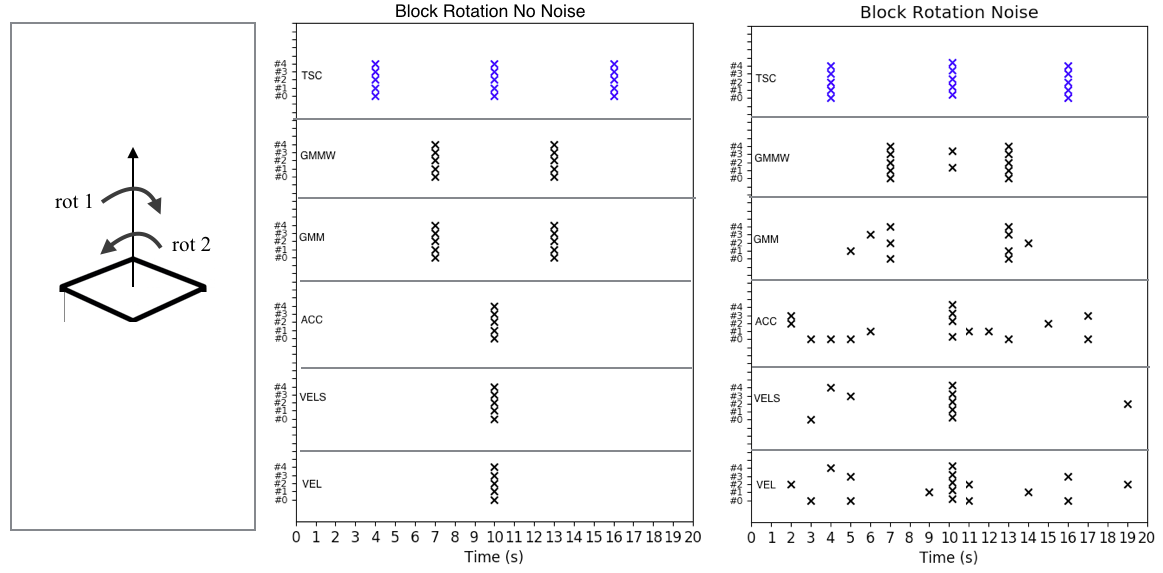
\includegraphics[width=\columnwidth]{tsc-experiments/block-results2.png}
\caption{Plots the identified transitions with each segmentation algorithm with and without noise. While all techniques are precise when there is no noise, \tsc is the most robust in the presence of noise but finds additional segments. \label{block-results}}
% \vspace{-1em}
\end{figure}


We apply the segmentation algorithms to 5 trajectories and plot the results in Figure \ref{block-results}.
As before, with no noise, all of the techniques are equally precise.
In this example, there is a difference between how the different techniques segment the trajectories.
The rate-of-change methods segment the trajectory at the point when the block changes rotation direction.
The GMM and the windowed GMM approaches cuts the trajectory into 3 even segments--missing the direction change.
\tsc cuts the trajectory into 4 segments including the direction change.
\tsc differs from the windowed GMM because it sets the number of clusters using the Dirichlet Process prior.
With noise, the rate-of-change techniques have a number of spurious segments.
The GMM-based approaches are more robust and \tsc improves the windowed GMM even further by clustering the detected transitions.
However, if the initial transitions were found in angular space, then \tsc would have found one segment.
In this sense, the definition of the state-space changes the segments found.
We hope to explore these issues in more detail in future work.


\begin{figure}[ht!]%[t]
\centering
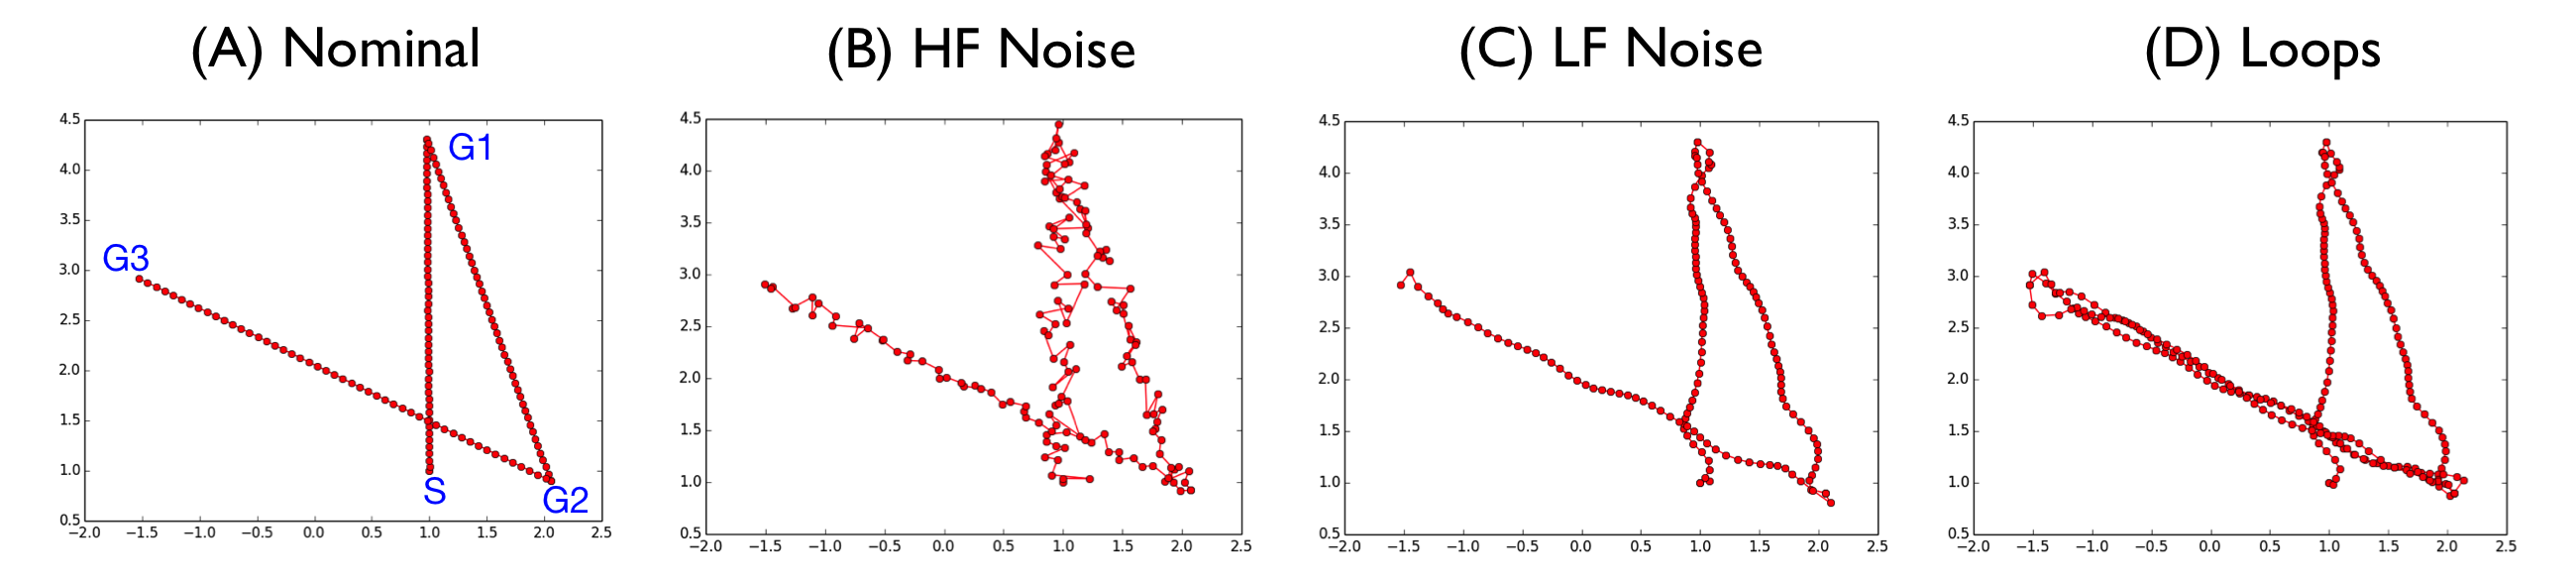
\includegraphics[width=\textwidth]{tsc-experiments/tsc_segmentation_benchmark.png}
\caption{One of 20 instances with random goal points $G1$, $G2$, $G3$. (a) Observations from a simulated demonstration with three regimes, (b) Observations corrupted with Gaussian white sensor noise, (c) Observations corrupted with low frequency process noise, and (d) Observations corrupted with an inserted loop. See Figure~\ref{exp3} for evaluation on loops. \label{simulated}}
% \vspace{-1em}
\end{figure}

\begin{figure}[ht!]%[t]
\centering
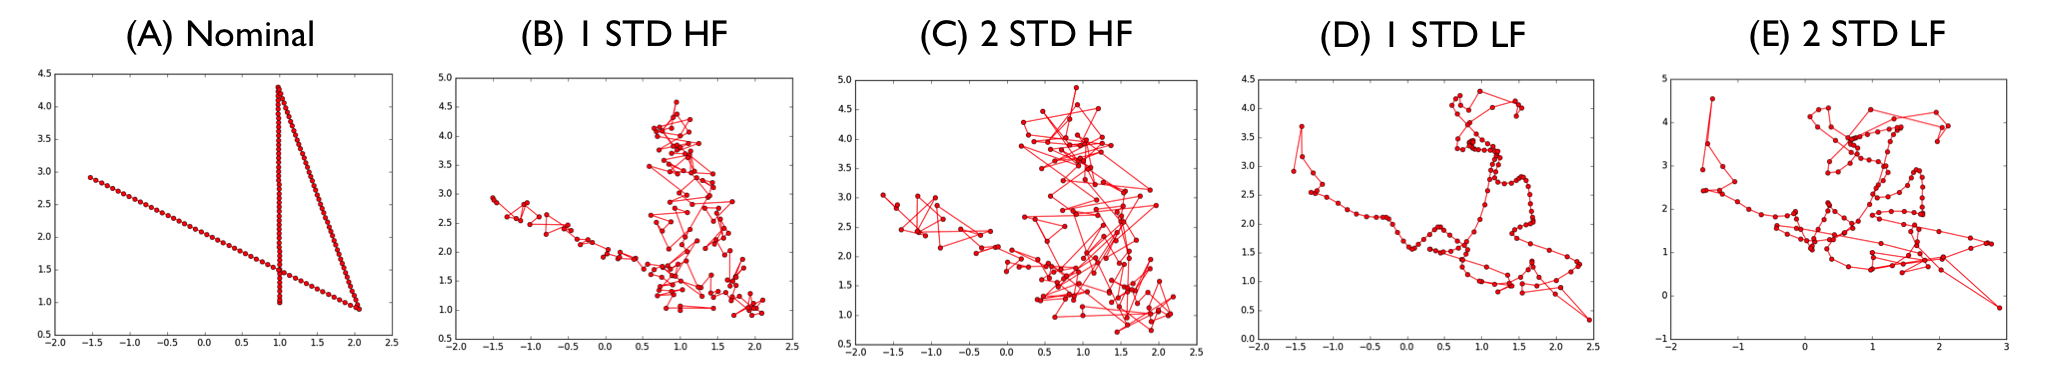
\includegraphics[width=\textwidth]{tsc-experiments/noise_illustration.png}
\caption{(a) Nominal trajectory, (b) 1 std. of high frequency observation noise, (c) 2 std. of high frequency observation noise,  (d) 1 std. of low frequency process noise, and (e) 2 std. of low frequency process noise. \label{simulated-noise}}
% \vspace{-1em}
\end{figure}

\subsubsection{Recall in Synthetic Examples}
Comparing different segmentation models can be challenging due to differing segmentation criteria. However, we identified some algorithms that identify locally linear or near linear segments.
We developed a synthetic dataset generator to generate piecewise linear segments and compared the algorithms on the generated dataset.
Note, we do not intend this to be a comprehensive evaluation of the accuracy of the different techniques, but more a characterization of the approaches on a locally linear example to study the key tradeoffs.

We model the trajectory of a point robot with two-dimensional position state $(x,y)$ between $k$ goal points $\{g_1,...,g_k\}$. 
We apply position control to guide the robot to the targets and without disturbance, this motion is linear (Figure \ref{simulated}a).
We add various types of disturbances (and in varying amounts) including Gaussian observation noise, low-frequency process noise, and repetitive loops (Figure \ref{simulated}b-d).
We report noise values in terms of standard deviations. Figure \ref{simulated-noise} illustrates the relative magnitudes.
A demonstration $d_i$ is a sample from the following system.

\vspace{0.5em}
\noindent\textbf{Task: } Every segmentation algorithm will be evaluated in its ability to identify the $k-1$ segments (i.e., the paths between the goal points).
Furthermore, we evaluate algorithms on random instances of this task.
In the beginning, we select $3$ random goal points.
From a fixed initial position, we control the simulated point robot to the goal points with position control. 
Without any disturbance, this follows a linear motion.
For a given noise setting, we sample demonstrations from this system and apply/evaluate each algorithm.
We present results aggregated over 20 such random instances.
This is important since many of the segmentation algorithms proposed in literature have some crucial hyper-parameters, and we present results with a \emph{single} choice of parameters averaged over multiple tasks.
This way, the hyper-parameter tuning cannot overfit to any given instance of the problem and has to be valid for the entire class of tasks.
We believe that this is important since tuning these hyper-parameters in practice (i.e., not in simulation) is challenging since there is no ground truth. 
The experimental code is available at: \url{http://berkeleyautomation.github.io/tsc/}.

\vspace{0.5em}
\noindent\textbf{5 Algorithms: } We compare \tsc against alternatives where the authors explicitly find (or approximately find) locally linear segments. It is important to reiterate that different segmentation techniques optimize different objectives, and this benchmark is meant to characterize the performance on a common task. All of the techniques are based on Gaussian Distributions or Linear auto-regressive models.


\begin{enumerate}
    \item \emph{(GMM)} (Same as previous experiment). In this experiment, we set the parameter to the optimal choice of $3$ without automatic tuning.
    \item \emph{(GMM+HMM)} A natural extension to this model is to enforce a transition structure on the regimes with a latent Markov Chain~\cite{asfour2006imitation,calinon2004stochastic,kruger2010learning, vakanski2012trajectory}. 
    We use the same state vector as above, without time augmentation as this is handled by the HMM. We fit the model using the forward-backward algorithm.
    \item \emph{Coresets} (Same as previous experiment).
    \item \emph{HSMM} We evaluated a Gaussian Hidden Semi-Markov Model as used in \cite{tanwani2016learning}. We directly applied this model to the demonstrations with no augmentation or normalization of features. This was implemented with the package \textsf{pyhsmm}. We directly applied this model to the demonstrations with no augmentation as in the GMM approaches. We ran our MCMC sampler for 10000 iterations, discarding the first 2500 as burn-in and thinning the chain by 15. 
    \item \emph{AR-HMM} We evaluated a Bayesian Autoregressive HMM model as used in \cite{niekum2012learning}. This was implemented with the packages \textsf{pybasicbayes} and \textsf{pyhsmm-ar}. The autoregressive order was $10$ and we ran our MCMC sampler for 10000 iterations, discarding the first 2500 as burn-in and thinning the chain by 15. 
\end{enumerate}

\vspace{0.5em}
\noindent\textbf{Evaluation Metric: } There is considerable debate on metrics to evaluate the accuracy of unsupervised segmentation and activity recognition techniques, e.g. frame accuracy ~\citep{wu2015watch}, hamming distance~\citep{fox2009sharing}. Typically, these metrics have two steps: (1) segments to ground truth correspondence, and (2) then measuring the similarity between corresponded segments. We have made this feature extensible and evaluated some different accuracy metrics (Jaccard Similarity, Frame Accuracy, Segment Accuracy, Intersection over Union). We found that the following procedure led to the most insightful results--differentiating the different techniques.

In the first phase, we match segments in our predicted sequence to those in the ground truth. We do this with a procedure identical to the one proposed in~\cite{wu2015watch}. We define a bi-partite graph of predicted segments to ground truth segments, and add weighted edges where weights represent the overlap between a predicted segment and a ground-truth segment (i.e., the recall over time-steps). Each predicted segment is matched to its highest weighted ground truth segment. Each predicted segment is assigned to exactly one ground-truth segment, while a ground-truth segment may have none, one, or more corresponding predictions.

After establishing the correspondence between predictions and ground truth, we consider a true positive (a ground-truth segment is correctly identified) if the overlap (intersection-over-union) between the ground-truth segment and its corresponding predicted segments is more than a default threshold 60\%.  Then, we compute \textsf{Segment Accuracy} as the ratio of the ground-truth segments that are correctly detected. In~\cite{wu2015watch}, the authors use a 40\% threshold but apply the metric to real data. Since this is a synthetic example, we increase this threshold to 60\%, which we empirically found accounted for boundary effects especially in the Bayesian approaches (i.e., repeated transitions around segment endpoints).

% In the second phase, we count the number of prediction-ground truth pairs where the intersection-over-union of time-steps is greater than 0.6 (a corresponded segment is predicted with at least 60\% accuracy). 
% We call this metric \textsf{Segment Accuracy} as in~\cite{wu2015watch}.
% The reported metric is an average over all predicted segments. 

%\subsubsection{Overview}

\subsubsection{Accuracy vs. Noise}
In our first experiment, we measured the segment accuracy for each of the algorithms for 50 demonstrations.
We also varied the amount of process and observation noise in the system.
As Figure \ref{simulated-noise} illustrates, this is a very significant amount of noise in the data, and successful techniques must exploit the structure in multiple demonstrations.
Figure \ref{exp1}a illustrates the performance of each of the techniques as a function of high-frequency observation noise.
Results suggest that \tsc is more robust to noise than the alternatives (nearly 20\% more accurate for 2.5 std of noise).
The Bayesian ARHMM approach is nearly identical to \tsc when the noise is low but quickly loses accuracy as more noise is added.
We attribute this robustness to the \tsc's pruning step which ensures that only transition state clusters with sufficient coverage across all demonstrations are kept.
These results are even more pronounced for low-frequency process noise (Figure \ref{exp1}b). \tsc is 49\% more accurate than all competitors for 2.5 std of noise added.
We find that the Bayesian approaches are particularly susceptible to such noise.
Furthermore, Figure \ref{exp1}c shows \tsc requires no more data than the alternatives to achieve such robustness.
Another point to note is that \tsc is solved much more efficiently than ARHMM or HSMM which require expensive MCMC samples.
While parameter inference on these models can be solved more efficiently (but approximately) with Mean-Field Stochastic Variational Inference, we found that the results were not as accurate.
\tsc is about 6x slower than using Coresets or the direct GMM approach, but it is over 100x faster than the MCMC for the ARHMM model.
Figure \ref{runtime} compares the runtime of each of the algorithms as a function of the number of demonstrations.

\begin{figure}[ht!]
\centering
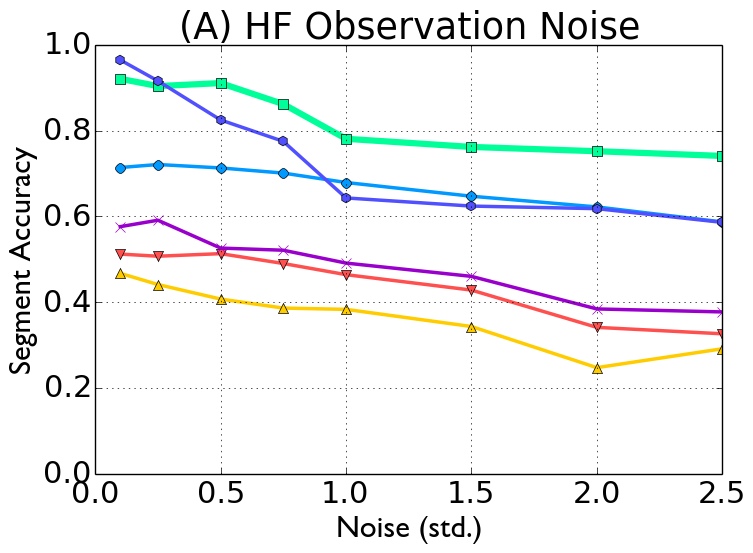
\includegraphics[width=0.32\textwidth]{tsc-experiments/exp1.png}
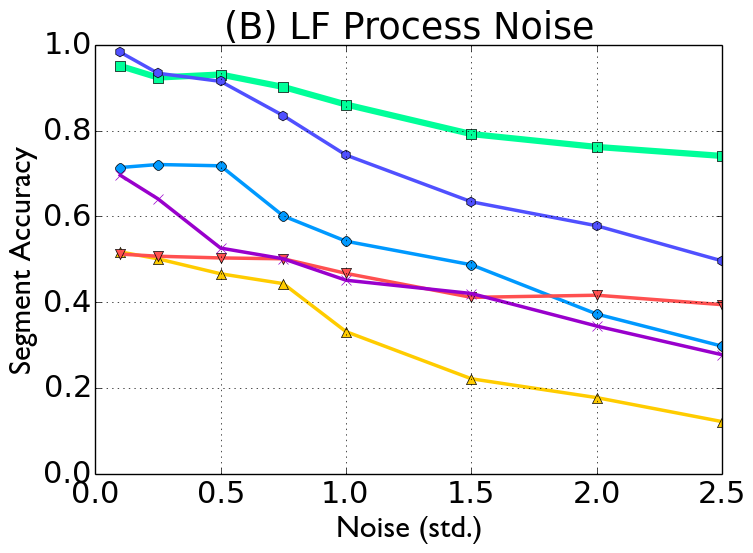
\includegraphics[width=0.32\textwidth]{tsc-experiments/exp2.png}
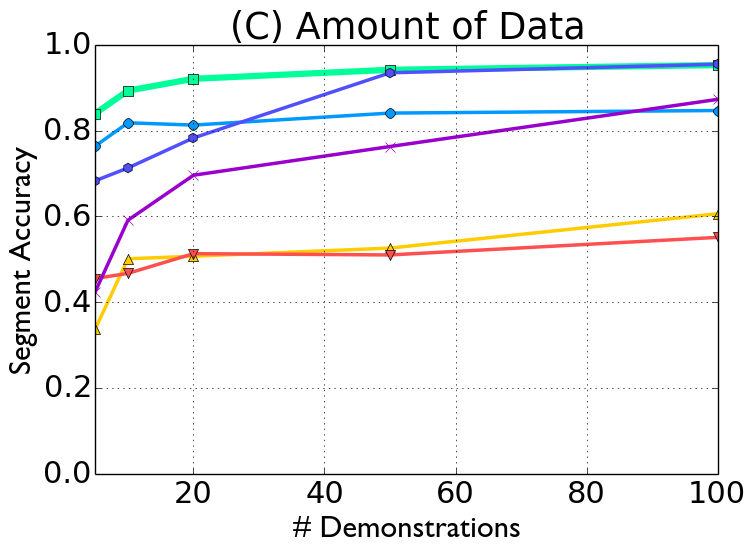
\includegraphics[width=0.32\textwidth]{tsc-experiments/exp5.png}
%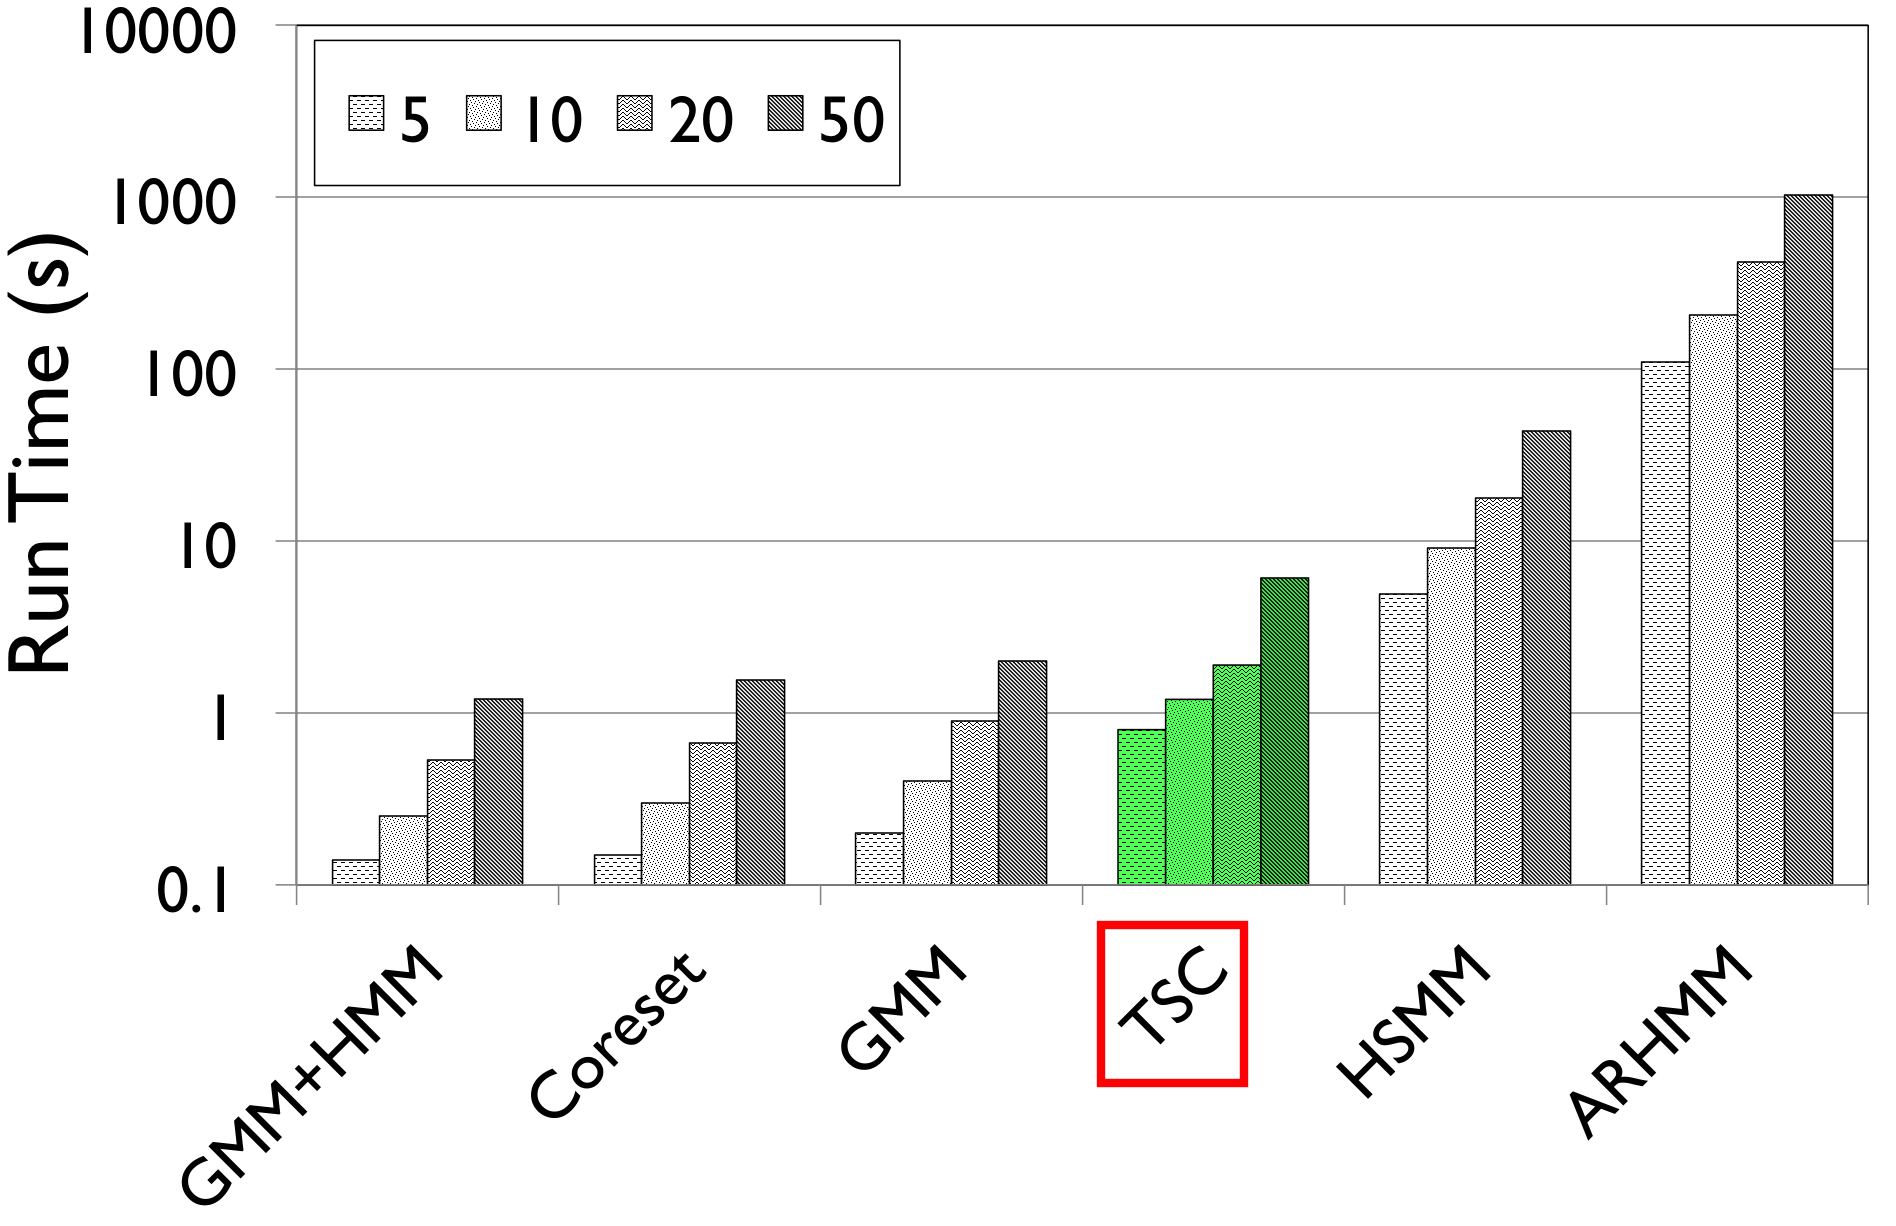
\includegraphics[width=0.24\textwidth]{tsc-experiments/bw_runtime.png}
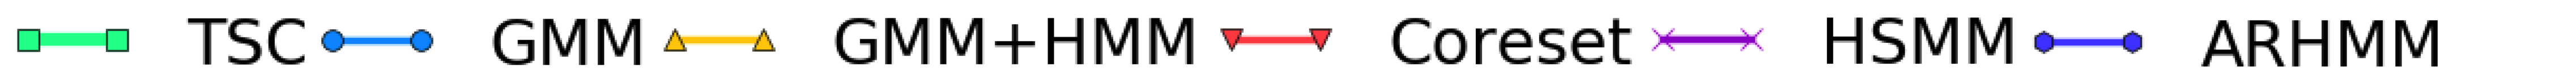
\includegraphics[width=0.8\textwidth]{tsc-experiments/big-legend.png}
\caption{Each data point represents 20 random instances of a 3-segment problem with varying levels of high-frequency noise, low-frequency noise, and demonstrations. We measure the segmentation accuracy for the compared approaches. (A) \tsc finds a more a accurate segmentation than all of the alternatives even under significant high-frequency observation noise, (B) \tsc is more robust to low-frequency process noise than the alternatives, 
% (C) \todo {\tsc performance on data with noisy loops.}
(C) the Bayesian techniques solved with MCMC (ARHMM, HSMM) are more sensitive to the number of demonstrations provided than the others.
%(D) \tsc runs over a 100x faster than the nearest alternative in terms of accuracy (ARHMM).  
\label{exp1}}
\end{figure}

\begin{figure}[ht!]
\centering
\includegraphics[width=0.8\columnwidth]{tsc-experiments/bw_runtime.png}
\caption{\tsc is about 6x slower than using Coresets or the direct GMM approach, but it is over 100x faster than the MCMC for the ARHMM model.\label{runtime}}
\end{figure}


\textbf{\tsc Hyper-Parameters: }
Next, we explored the dependence of the performance on the hyper-parameters for \tsc.
We focus on the window size and the pruning parameter.
Figure \ref{exp3}a shows how varying the window size affects the performance curves.
Larger window sizes can reject more low-frequency process noise.
However, larger windows are also less efficient when the noise is low.
Similarly, Figure \ref{exp3}b shows how increasing the pruning parameter affects the robustness to high-frequency observation noise.
However, a larger pruning parameter is less efficient at low noise levels. 
Based on these curves, we selected $(w=3, \rho=0.3)$ in our synthetic experiments.

\begin{figure}[ht!]
\centering
\includegraphics[width=0.48\columnwidth]{tsc-experiments/exp3.png}
\includegraphics[width=0.48\columnwidth]{tsc-experiments/exp4.png}
\caption{(A) shows the performance curves of different choices of windows as a function of the process noise. Larger windows can reject higher amounts of process noise but are less efficient at low noise levels. (B) the performance curves of different choices of the pruning threshold. Larger pruning thresholds are more robust to high amounts of observation noise but less accurate in the low noise setting. We selected $(w=3, \rho=0.3)$ in our synthetic experiments. \label{exp3}}
\end{figure}

\textbf{Loops: }
Finally, we evaluated 4 algorithms on how well they can detect and adjust for loops.
\tsc compacts adjacent motions that are overly similar, while HMM-based approaches correspond similar looking motions.
An HMM grammar over segments is clearly more expressive than \tsc's, and we explore whether it is necessary to learn a full transition structure to compensate for loops.
We compare the accuracy of the different segmentation techniques in detecting that a loop is present (Figure \ref{exp4}).
Figure \ref{exp4}a shows that \tsc is competitive with the HMM approaches as we vary the observation noise; however, the results suggest that ARHMM provides the most accurate loop detection.
On the other hand, Figure \ref{exp4}b suggests that process noise has a very different effect.

\begin{figure}[ht!]
\centering
\includegraphics[width=0.48\columnwidth]{tsc-experiments/exp6.png}
\includegraphics[width=0.48\columnwidth]{tsc-experiments/exp7.png}
\caption{(A) illustrates the accuracy of \tsc's compaction step as a function of observation noise. \tsc is competitive with the HMM-based approaches without having to model the full transition matrix. (B) \tsc is actually more robust to low-frequency process noise in the loops than the HMM-based approaches. \label{exp4}}
\end{figure}
\tsc is actually more accurate than the HMM approaches when the process noise is high--even without learning a transition structure.

\textbf{Scaling with Dimensionality: }
We investigate how the accuracy of \tsc scales with the dimensionality of the state-space.
As in the previous experiments, we measured the segment accuracy for each of the algorithms for 50 demonstrations.
This time we generated the line segments in increasingly higher dimensional spaces (from 2-D to 35-D).
The noise added to the trajectories has a std of 0.1.
Figure \ref{exps}a plots the segment accuracy as a function of the dimensionality of the state-space.
While the accuracy of \tsc does decreases as the dimensionality increases it is more robust than some of the alternatives: ARHMM and HSMM.
One possible explanation is that both of those techniques rely on Gibbs Sampling for inference, which is a little more sensitive to dimensionality than the expectation-maximization inference procedure used in GMM and GMM+HMM.
Figure \ref{exps}b shows one aspect of \tsc that is more sensitive to the dimensionality.
The loop compaction step requires a dynamic time-warping and then a comparison to fuse repeated segments together.
This step is not as robust in higher dimensional state-spaces.
This is possibly due to the use of the $L_2$ distance metric to compare partial trajectories to compact.
\tsc runs in $4$ seconds on the 2-D case, $16$ seconds on the 10-D case, and in $59$ seconds on the 35-D case. 


\begin{figure}[ht!]
\centering
\includegraphics[width=0.48\columnwidth]{tsc-experiments/exp11.png}
\includegraphics[width=0.48\columnwidth]{tsc-experiments/exp12.png}
\caption{We investigate how the accuracy of \tsc scales with the dimensionality of the state-space. In (A) we consider the problem with no loops or compaction, and in  (B) we measure the accuracy of the compaction step as a function of dimensionality. \label{exps}}
\end{figure}


\subsection{Surgical Data Experiments}
We describe the three tasks used in our evaluation and the corresponding manual segmentation (Figure \ref{demo}).
This will serve as ground truth when qualitatively evaluating our segmentation on real data.
This set of experiments primarily evaluates the utility of segments learned by \tsc.
Data was collected before hand as a part of prior work.
Our hypothesis is that even though \tsc is unsupervised, it identifies segments that often align with manual annotations.
In all of our experiments, the pruning parameter $\rho$ is set to $80\%$ and the compaction heuristic $\delta$ is to 1cm.

\begin{figure}[ht!]
\centering
\includegraphics[width=0.7\textwidth]{tsc-experiments/conceptual_plots}
 \caption{Hand annotations of the three tasks: (a) circle cutting, (b) needle passing, and (c) suturing. Right arm actions are listed in dark blue and left arm actions are listed in yellow. \label{demo}}
%  \vspace{-2em}
\end{figure}


The state-space is the 6D end-effector position.
In some experiments, we augment this state-space with the following visual features:
\begin{enumerate}
\item \emph{Grasp}. 0 if empty, 1 otherwise.
\item \emph{Needle Penetration}. We use an estimate of the penetration depth based on the robot kinematics to encode this feature. 
If there is no penetration (as detected by video), the value is 0, otherwise the value of penetration is the robot's $z$ position.
\end{enumerate}
Our goal with these features was to illustrate that \tsc applies to general state-spaces as well as spatial ones, and not to address the perception problem.
These features were constructed via manual annotation, where the Grasp and Needle Penetration were identified by reviewing the videos and marking the frames at which they occurred.

\vspace{0.5em}

\noindent\textbf{Circle Cutting: }
A 5 cm diameter circle drawn on a piece of gauze.
The first step is to cut a notch into the circle.
The second step is to cut clockwise half-way around the circle.
Next, the robot transitions to the other side cutting counter clockwise.
Finally, the robot finishes the cut at the meeting point of the two cuts.
As the left arm's only action is to maintain the gauze in tension, we exclude it from the analysis. 
In Figure \ref{demo}a, we mark 6 manually identified transitions points for this task from \cite{murali2015learning}: (1) start, (2) notch, (3) finish 1st cut, (4) cross-over, (5) finish 2nd cut, and (6) connect the two cuts.
For the circle cutting task, we collected 10 demonstrations by researchers who were not surgeons but familiar with operating the da~Vinci Research Kit~(dVRK).

\vspace{0.5em}
We also perform experiments using the JIGSAWS dataset~\cite{gao2014jigsaws} consisting of surgical activity for human motion modeling. The dataset was captured using the da Vinci Surgical System from eight surgeons with different levels of skill performing five repetitions each of Needle Passing and Suturing.

\vspace{0.5em}

\noindent\textbf{Needle Passing: } We applied \tsc to 28 demonstrations of the needle passing task.
The robot passes a needle through a hoop using its right arm, then its left arm to pull the needle through the hoop. Then, the robot hands the needle off from the left arm to the right arm. This procedure is repeated four times as illustrated with a manual segmentation in Figure~\ref{demo}b.

\vspace{0.5em}

\noindent\textbf{Suturing: }Next, we explored 39 examples of a 4 throw suturing task (Figure \ref{demo}c). Using the right arm, the first step is to penetrate one of the points on right side. The next step is to force the needle through the phantom to the other side. Using the left arm, the robot pulls the needle out of the phantom and then the robot hands it off to the right arm for the next point. 



\subsubsection{Results}\label{results:real}

\noindent\textbf{Circle Cutting: }
Figure\,\ref{exp:circ}a shows the transition states obtained from our algorithm. And Figure\,\ref{exp:circ}b shows the \tsc clusters learned (numbered by time interval midpoint).
The algorithm found 8 clusters, one of which was pruned using our $\rho=80\%$ threshold rule.

The remaining 7 clusters correspond well to the manually identified transition points.
It is worth noting that there is one extra cluster (marked $2'$), that does not correspond to a transition in the manual segmentation.
At $2'$, the operator finishes a notch and begins to cut.
While at a logical level notching and cutting are both penetration actions, they correspond to two different linear transition regimes due to the positioning of the end-effector.
Thus, \tsc separates them into different clusters even though the human annotators did not.
This illustrates why supervised segmentation is challenging.
Human annotators segment trajectories on boundaries that are hard to characterize mathematically, e.g., is frame 34 or frame 37 the segment boundary.
Supervisors may miss crucial motions that are useful for automation or learning.

\begin{figure}[ht!]
    \includegraphics[width=\columnwidth]{tsc-experiments/new_circle_cutting}
    \caption{(a) The transition states for the circle cutting task are marked in black. (b) The \tsc clusters, which are clusters of the transition states, are illustrated with their 75\% confidence ellipsoid.\label{exp:circ}}
\end{figure}



% \vspace{0.5em}

\noindent\textbf{Needle Passing: } 
In Figure\,\ref{exp:np}a, we plot the transition states in $(x,y,z)$ end-effector space for both arms.
We find that these transition states correspond well to the logical segments of the task (Figure\,\ref{demo}b).
These demonstrations are noisier than the circle cutting demonstrations, and there are more outliers.
The subsequent clustering finds 9 clusters (2 pruned).
Next, Figures\,\ref{exp:np}b-c illustrate the \tsc clusters.
We find that again \tsc learns a small parametrization for the task structure with the clusters corresponding well to the manual segments.
However, in this case, the noise does lead to a spurious cluster (4 marked in green).
One possible explanation is that the demonstrations contain many adjustments to avoid colliding with the needle hoop and the other arm while passing the needle through leading to numerous transition states in that location.

\begin{figure}[ht!]
\centering
    \includegraphics[width=0.8\textwidth]{tsc-experiments/new_needle_passing2.eps}
    \vspace{-0.7em}
    \caption{(a) The transition states for the task are marked in orange (left arm) and blue (right arm). (b-c) The \tsc clusters, which are clusters of the transition states, are illustrated with their 75\% confidence ellipsoid for both arms}
    \label{exp:np}
    \vspace{-0.5em}
\end{figure}


%Our technique is not limited to x,y,z states for the robot and works with more general configurations. In Figure \ref{exp:np}b, at each of the first 5 clusters, we plot the learned mean pose. 
%This shows that the robot has to orient its end-effector horizontal to the loop during the pass through and pull and vertical during the handoff.

\vspace{0.5em}

\noindent\textbf{Suturing: }
In Figure\,\ref{exp:su}, we show the transition states and clusters for the suturing task.
As before, we mark the left arm in orange and the right arm in blue.
This task was far more challenging than the previous tasks as the demonstrations were inconsistent.
These inconsistencies were in the way the suture is pulled after insertion (some pull to the left, some to the right, etc.), leading to transition states all over the state space. 
Furthermore, there were numerous demonstrations with looping behaviors for the left arm.
In fact, the DP-GMM method gives us $23$ clusters, $11$ of which represent less than $80$\% of the demonstrations and thus are pruned (we illustrate the effect of the pruning in the next section).
In the early stages of the task, the clusters clearly correspond to the manually segmented transitions.
As the task progresses, we see that some of the later clusters do not.


\begin{figure}[ht!t]
\centering
    \includegraphics[width=0.8\textwidth]{tsc-experiments/new_suturing2.eps}
    \vspace{-0.7em}
    \caption{ (a) The transition states for the task are marked in orange (left arm) and blue (right arm). (b-c) The clusters, which are clusters of the transition states, are illustrated with their 75\% confidence ellipsoid for both arms}
    \label{exp:su}
    % \vspace{-0.5em}
\end{figure}


\begin{table*}
\caption{This table compares transitions learned by \tsc and transitions identified by manual annotators in the JIGSAWS dataset. We found that the transitions mostly aligned. $83\%$ and $73\%$ of transition clusters for needle passing and suturing respectively contained exactly one surgeme transition when both kinematics and vision were used. Results suggest that the hierarchical clustering is more suited for mixed video and kinematic feature spaces.}
\centering
\scriptsize
\begin{tabular}{| l | c | c | c | c | c |}
\hline
 & No. of Surgeme Segments & No. of Clusters & seg-surgeme & surgeme-seg \\ 
\hline
Needle Passing TSC(Kin+Video)  & $14.4 \pm 2.57$ & 11 & 83\% & 74\% \\ \hline
Needle Passing TSC(Video) & $14.4 \pm 2.57$ & 7 & 62\% & 69\% \\ \hline
Needle Passing TSC(Kin) & $14.4 \pm 2.57$ & 16 & 87\% & 62\% \\ \hline
Needle Passing TSC(VELS) & $14.4 \pm 2.57$ & 13 & 71\% & 70\% \\ \hline
Needle Passing TSC(No-H)  & $14.4 \pm 2.57$ & 5 & 28\% & 34\% \\\hline
\hline
Suturing TSC(Kin+Video) & $15.9 \pm 3.11$ & 13 & 73\% & 66\% \\ \hline
Suturing TSC(Video) & $15.9 \pm 3.11$ & 4 & 21\% & 39\% \\ \hline
Suturing TSC(Kin) & $15.9 \pm 3.11$ & 13 & 68\% & 61\% \\ \hline
Suturing TSC(VELS) & $15.9 \pm 3.11$ & 17 & 48\% & 57\% \\ \hline
Suturing TSC(No-H) & $15.9 \pm 3.11$ & 9 & 51\% & 52\% \\ \hline
\end{tabular}
 \label{exp:surgemes}
\end{table*}


\subsubsection{Comparison to Surgemes}
%\todo{SK: Clean up the metrics}
Surgical demonstrations have an established set of primitives called surgemes, and we evaluate if segments discovered by our approach correspond to surgemes. 
In Table \ref{exp:surgemes}, we compare the number of \tsc segments for needle passing and suturing to the number of annotated surgeme segments.
We apply different variants of the \tsc algorithm and evaluate its ability to recover segments similar to surgemes.
We consider: (Kin+Video) which is the full \tsc algorithm, (Kin) which only uses kinematics, (Video) which only uses the visual annotations, (VELS) which uses the zero-crossing velocity heuristic to get the initial transitions, and (NO-H) which treats all of the variables as one big feature space and does not hierarchically cluster.
A key difference between our segmentation and number of annotated surgemes is our compaction and pruning steps.
To account for this, we first select a set of surgemes that are expressed in most demonstrations (i.e., simulating pruning), and we also apply a compaction step to the surgeme segments.
When surgemes appear consecutively, we only keep the one instance of each.
We explore two metrics: \textbf{seg-surgeme} the fraction of \tsc clusters with only one surgeme switch (averaged over all demonstrations), and \textbf{surgeme-seg} the fraction of surgeme switches that fall inside exactly one \tsc cluster.

 We found that the transitions learned by \tsc with both the kinematic and video features were the most aligned with the surgemes. 
 $83\%$ and $73\%$ of transition clusters for needle passing and suturing respectively contained exactly one surgeme transition when both were used.
 For the needle passing task, we found that the video features alone could give a reasonably accurate segmentation.
 However, this did not hold for the suturing dataset.
 The manual video features are low dimensional and tend to under-segment.
 For the suturing dataset, a combination of the visual and kinematic features was most aligned with the surgemes.
 Similarly, this scaling problem affects the variant that does not hierarchically cluster--leading to a small number of clusters--and inaccuracy.
 
 
 
\subsubsection{Pruning and Compaction} \label{sec:pruningCompaction}
In Figure \ref{exp:removal}, we highlight the benefit of pruning and compaction using the Suturing task as exemplar.
First, we show the transition states without applying the compaction step to remove looping transition states (Figure \ref{exp:removal}a).
We find that there are many more transition states at the ``insert" step of the task.
Compaction removes the segments that correspond to a loop of the insertions.
Next, we show all of the clusters found by the first step of segmentation.
The centroids of these clusters are marked in Figure \ref{exp:removal}b.
In all, 11 clusters are pruned by this rule.

% \begin{figure}[ht!t]
%     \centering
%     \includegraphics[width=0.35\textwidth]{tsc-experiments/suturing_milestones_no_compaction}
%     \includegraphics[width=0.35\textwidth]{tsc-experiments/suturing_milestones_no_pruning}
%     \caption{We illustrate the benefits of pruning small clusters and our retry compaction algorithm. We first show the transition states without compaction, and then show the clusters without pruning.}
%      \label{exp:removal}
% \end{figure}

\begin{figure}[ht!]
    \centering
    \includegraphics[width=0.35\columnwidth]{tsc-experiments/suturing_milestones_no_compaction}
    \includegraphics[width=0.35\columnwidth]{tsc-experiments/suturing_milestones_no_pruning}
    \caption{We first show the transition states without compaction (in black and green), and then show the clusters without pruning (in red). Compaction sparsifies the transition states and pruning significantly reduces the number of clusters.}
    \label{exp:removal}
\end{figure}
 
\subsection*{TSC with Deep Features}
Inspired by the recent success of deep neural networks in reinforcement learning~\cite{levine2015end, lenz2015deep}, we then explored how visual features extracted from Convolutional Neural Networks can be used for transition state identification.

We use layers from a pre-trained Convolutional Neural Network (CNNs) to derive the features frame-by-frame. In particular, we explore two architectures designed for image classification task on natural images: (a) \textbf{AlexNet: } Krizhevsky et al. proposed multilayer (5 in all) a CNN architecture \cite{krizhevsky2012imagenet}, and (b)~\textbf{VGG: } Simoyan et al. proposed an alternative architecture termed VGG (acronym for Visual Geometry Group) which increased the number of convolutional layers significantly (16 in all)~\cite{simonyan2014very}. In our experiments, we explore the level of generality of features required for segmentation. We also compare these features to other visual featurization techniques such as SIFT for the purpose of task segmentation using \tsc. 


\subsubsection{Evaluation of Visual Featurization}
In our first experiment, we explore different visual featurization, encoding, and dimensionality reduction techniques.
We applied \tsc to our suturing experimental dataset and measured the silhouette score of the resulting transition state clusters.
On this dataset, our results suggest that features extracted from the pre-trained CNNs resulted in tighter transition state clusters compared to SIFT features with a 3\% lower \textsf{ss} than the worst CNN result.
We found that features extracted with the VGG architecture resulted in the highest \textsf{ss} with a 3\% higher \textsf{ss} than the best AlexNet result.
We also found that PCA for dimensionality reduction achieved a \textsf{ss} performance of 7\% higher than the best GRP result and 10\% higher than best CCA result.
Because CCA finds projections of high correlation between the kinematics and video, we believe that CCA discards informative features resulting in reduced clustering performance. 
We note that neither of the encoding schemes, VLAD or LCD\del{LCD$_{VLAD}$} significantly improves the \textsf{ss}.

There are two hyper-parameters for \tsc which we set empirically: sliding window size (T = 3), and the number of PCA dimensions (k = 100).
In Figure \ref{fig:sensitvity}, we show a sensitivity plot with the \textsf{ss} as a function of the parameter.
We calculated the \textsf{ss} using the same subset of the suturing dataset as above and with the VGG conv5\_3 CNN.
We found that T = 3 gave the best performance.
We also found that PCA with k = 1000 dimensions was only marginally better than k = 100 yet required $>$30 mins to run.
For computational reasons, we selected k = 100.


\begin{figure}[ht!]
% \vspace{-10pt}
\centering
    \includegraphics[width=0.95\linewidth]{tsc-experiments/sensitivity}
    \caption{We evaluate the sensitivity of two hyperparameters set in advance: number of PCA dimensions and sliding window size. The selected value is shown in red double circles.\label{fig:sensitvity}}
% \vspace{-10pt}
\end{figure}


\subsubsection{t-SNE visualization of visual features}
One of the main insights of this study is that features from pre-trained CNNs exhibit locally-linear behavior which allows application of a switching linear dynamical system model. 
% One of the main insights of this paper is that, surprisingly, trajectories of convolutional features sometimes exhibit the necessary local-linearity needed to apply Transition State Clustering.
We experimentally tested this by applying dimensionality reduction to trajectories of features from different video featurization techniques.
Figure \ref{fig:tsne} shows t-SNE embeddings of visual features extracted for a single demonstration of suturing. The deep features display clear locally-linear properties and can be more easily clustered than SIFT features extracted for the corresponding frames. 
We speculate that SIFT breaks up trajectory structure due to its natural scale and location invariance properties.
We also compared to using the raw RGB image pixel values and discovered that the deep features result in more well-formed locally linear trajectories.
However, it is important to note that unlike spatial trajectories there are discrete jumps in the convolutional trajectories.
We hope to explore this problem in more detail in future work.

\begin{figure}[!ht]
\centering
    \includegraphics[width=0.45\linewidth]{tsc-experiments/t-SNE_suturing_v3}
    \caption{Each data point in the figure corresponds to a t-SNE visualization of features of a single frame in the video. (a) RGB pixel values of original image (b) shallow SIFT features (c) CNN features from AlexNet pool5 (d)  CNN features from VGG Conv5\_3.
    %The changepoints recovered from \tsc are highlighted as black triangles.
    \label{fig:tsne}}
\end{figure}

\subsubsection{End-to-End Evaluation}
For all subsequent experiments on real data, we used a pre-trained VGG CNN conv5\_3 and encoded with PCA with 100 dimensions. 


\vspace{0.25em}
\noindent\textbf{1. Suturing: } 
We apply our method to a subset of the JIGSAWS dataset~\cite{gao2014jigsaws} consisting of surgical task demonstrations under teleoperation using the da~Vinci surgical system. The dataset was captured from eight surgeons with different levels of skill, performing five repetitions each of suturing and needle passing.
\tabref{jigsaws} lists quantitative results for both needle passing and suturing with both \textsf{ss} and NMI agreement with the human labels.
Demonstrations from the JIGSAWS dataset were annotated with the skill-level of the demonstrators (Expert (E), Intermediate (I), and Novice (I)).
For the suturing dataset, we find that using both kinematics and video gives up-to 30.1\% improvement in \textsf{ss} and 52.3\% improvement in NMI over using kinematics alone.
Not surprisingly, we also find that the expert demonstrations, which are usually smoother and faster, lead to improved segmentation performance when using only the kinematic data.
However, when we incorporate the visual data, the trend is not as clear.
We speculate this has to do with the tradeoff between collecting more data (denser clusters and more accurate modeling) versus inconsistencies due to novice errors, and this tradeoff is evident in higher dimensional data.

We visualize the results of the segmentation on one representative trajectory~(Figure \ref{fig:suturing}).
With combined kinematics and vision, \tsc learns many of the important segments identified by annotation in \cite{gao2014jigsaws}.
Upon further investigation of the false positives, we found that they corresponded to meaningful actions missed by human annotators.
\tsc discovers that a repositioning step where many demonstrators penetrate and push-through the needle in two different motions.
While this is largely anecdotal evidence, we were able to find some explanations for some of the false positives found by \tsc.

%This emphasizes than manual annotation and pre-defined dictionary methods are sensitive to human bias and inconsistency in segmentation criteria.

% applies a more consistent criteria than manual annotation based on domain knowledge.

% ALL OF JIGSAWS RESULTS
\begin{figure}[!ht]
%\vspace{-10pt}
    \centering
    \includegraphics[width=\linewidth]{tsc-experiments/suturing-v4}
    \caption{The first row shows a manual segmentation of the suturing task in 4 steps: (1) Needle Positioning, (2) Needle Pushing, (3) Pulling Needle, (4) Hand-off. \tsc extracts many of the important transitions without labels and also discovers un-labled transition events.
    \label{fig:suturing}}
% \vspace{-15pt}
\end{figure}



\begin{figure}[!ht]
%\vspace{-10pt}
    \centering    
    \caption{Comparison of \tsc performance on Suturing and Needle Passing Tasks. We compare the prediction performance by incrementally adding demonstrations from Experts~(E), Intermediates~(I), and Novices~(N) respectively to the dataset.\label{tab:jigsaws}}
    \includegraphics[width=0.8\linewidth]{tsc-experiments/tsc-table.png}}
% \vspace{-15pt}
\end{figure}


\vspace{0.25em}
\noindent\textbf{2. Needle Passing: } Next, we applied \tsc to 28 demonstrations of the needle passing task.
These demonstrations were annotated in \cite{gao2014jigsaws}. 
In this task, the robot passes a needle through a loop using its right arm, then its left arm to pull the needle through the loop. Then, the robot hands the needle off from the left arm to the right arm. This is repeated four times. 
 Similar to the suturing dataset, we find that the combination of the features gives the best results.
 For the needle passing dataset, we find that using both kinematics and video gives up to 22.2\% improvement in \textsf{ss} and 49.7\% improvement in NMI over using the best of either kinematics or vision alone.

We found that the learned segments for the needle passing task were less accurate than those learned for the suturing task.
We speculate that this is due to the multilateral nature of this task.
This task uses both arms more than the suturing task, and as a result, there are many visual occlusions for a fixed camera. 
Important features such as the needle pose and the thread may be obscured at different points during the task.
Furthermore, we constructed the state-space using the states of both arms.
For such a task, it may be better to segment each of the arms independently.



%In this task, the robot passes a needle through a loop using its right arm, then its left arm to pull the needle through the loop. Then, the robot hands the needle off from the left arm to the right arm. This is repeated four times. 

% \begin{figure}[!t]
% \centering
% \includegraphics[width=\linewidth]{tsc-experiments/insert.png}
% \caption{The figure illustrates the performance of unsupervised segmentation of the 3 Step Lego Assembly Task performed with tele-operated PR2 with two techniques of manual demonstrations.}
%  \label{fig:lego-pr2}
% \vspace{-10pt} 
% \end{figure}

% \begin{figure}[!t]
% \centering
% \includegraphics[width=\linewidth]{tsc-experiments/insert.png}
% \caption{The figure illustrates the comparison of unsupervised segmentation of the Toy Example performed with tele-operated PR2 with two techniques of manual demonstrations.}
%  \label{fig:toyPlane-pr2human}
% \vspace{-10pt} 
% \end{figure}




\vspace{5pt}
\noindent \textbf{3. PR2: Legos and Toy Plane Assembly: }
In our next experiment, we explore segmenting a multi-step assembly task using (1) large \textit{Lego} blocks and (2) toy \textit{Plane} from the YCB dataset~\cite{calli2015corr}. 
We demonstrate that \tsc applies generally outside of surgical robotics.
We collect eight kinesthetic demonstrations for each task through kinesthetic demonstrations of the task on the PR2 robot.
Figure \ref{pr2toyplane} illustrates the segmentation for the plane assembly task.
We find the plane assembly task using kinematics or vision alone results in a large number of segments.
The combination can help remove spurious segments restricting our segments to those transitions that occur in most of the demonstrations--agreeing in similarity both kinematically and visually.


\begin{figure}[!t]
\centering
\includegraphics[width=\linewidth]{tsc-experiments/pr2_plane_assembly-v5}
\caption{We compare \tsc on 12 kinesthetic demonstrations (top) and
8 human demonstrations (bottom).
No kinematics were available for the human demonstrations.
We illustrate the segmentation for an example demonstration of each.
Our manual annotation of the task has five steps and \tsc recovers this structure separately for both Kinesthetic demos on PR2 and Human demos with the same visual features. \label{pr2toyplane}}
\end{figure}

% \subsubsection{Human Demonstration of Toy Plane Assembly}
\vspace{5pt}
\noindent \textbf{4. Human Demonstration of Toy Plane Assembly: }
We extend the toy plane assembly experiment to collect eight demonstrations each from two human users. These examples only have videos and no kinematic information. We note that there was a difference between users in the grasping location of fuselage. 
 We also \TSC to learn segmentation for human demonstrations.
The results of \tsc performance are summarized in Table~\ref{tab:pr2}.
We omit a visualization of the results for the Lego assembly. However, we summarize the results quantitatively in the table.

% one example each of the \textit{Lego} and \textit{Plane} assembly task is illustrated in Figures~\ref{fig:lego-pr2} and \ref{fig:pr2_toyplane} respectively.
% The results for clustering evaluation and comparison with a set of manual labels using dynamic time warping distance are tabulated in \tabref{pr2}.


% PR2 TABLE
\begin{table}[!t]
\centering
\resizebox{\linewidth}{!}{% put in textwidth
    \begin{tabular}{l|l|l|l}
        \hline
        \multicolumn{1}{c|}{}& \multicolumn{1}{c|}{K} & \multicolumn{1}{c|}{Z} & \multicolumn{1}{c}{K+Z} \\ \hline \hline 
        \multicolumn{4}{l}{Silhouette Score -- Intrinsic Evaluation}  \\
        Lego (Robot)    & 0.653$\pm$0.003 & 0.644$\pm$0.026 & 0.662$\pm$0.053 \\
         Plane (Robot)   & 0.741$\pm$0.011 & 0.649$\pm$0.007 & 0.771$\pm$0.067 \\
        Plane (Human 1) & -- & 0.601 $\pm$0.010  & -- \\ 
        Plane (Human 2) & -- & 0.628 $\pm$0.015  & -- \\ \hline \hline
        \multicolumn{4}{l}{NMI Score -- Extrinsic evaluation against manual labels}  \\ 
        Lego (Robot)    & 0.542 $\pm$ 0.058  & 0.712 $\pm$ 0.041  & 0.688 $\pm$ 0.037  \\
         Plane (Robot)   & 0.768 $\pm$ 0.015  & 0.726 $\pm$ 0.040  & 0.747 $\pm$ 0.016    \\ 
        Plane (Human 1) & -- & 0.726 $\pm$ 0.071  & -- \\ 
        Plane (Human 2) & -- & 0.806 $\pm$ 0.034  & -- \\ \hline
    \end{tabular} 
    }
\caption{Plane and Lego Assembly Tasks. Both tasks show improvements in clustering and prediction accuracy using multi-modal data as compared to either modality. Further, only vision ($Z$) is available for human demos of the plane assembly task. Comparable segmentation results are obtained using only video input for human demos. \textit{Higher} Silhoutte Scores and NMI scores are better, respectively. \label{tab:pr2}}
\vspace{-10pt}
\end{table}

\section{SWIRL: Learning With Transition States}
\label{swirl}
Next, we build on TSC to construct a planner that leverages the structure learned by TSC.
Real-world tasks often naturally decompose into a sequence of simpler, locally-solvable sub-tasks.
For example, an assembly task might decompose into completing the part's constituent sub-assemblies or a surgical task might decompose into a sequence of movement primitives.
Such structure imposes a strong prior on the class of successful policies and can focus exploration in reinforcement learning.
It reduces the effective time horizon of learning to the start of the next subtask rather than until task completion.
We apply a clustering algorithm to identify a latent set of state-space subgoals that sequentially compose to form the global task.
This leads to a novel policy search algorithm, called Sequential Windowed Inverse Reinforcement Learning (SWIRL),  where the demonstrations can bootstrap a self-supervised Q-learning algorithm.

 Transitions are defined as significant changes in the state trajectory. These transitions can be spatially and temporally clustered to identify if there are common conditions that trigger a change in motion across demonstrations.
SWIRL extends this basic model with an Inverse Reinforcement Learning step that extracts subgoals and computes local cost functions from the learned clusters. 
Learning a policy over the segmented task is nontrivial because solving $k$ independent problems neglects any shared structure in the value function during the policy learning phase (e.g., a common failure state).
Jointly learning over all segments introduces a dependence on history, namely, any policy must complete step $i$ before step $i+1$.
Learning a memory-dependent policy could lead to an exponential overhead of additional states. 
We show that the problem can be posed as a proper MDP in a lifted state-space that includes an indicator variable of the highest-index $\{1,...,k\}$ transition region that has been reached so far if there are Markovian regularity assumptions on the clustering algorithm.

\subsection*{Model and Notation}
Directly optimizing the reward function $\mathcal{R}$ in the MDP from the previous section might be very challenging.
We propose to approximate $\mathcal{R}$ with a sequence of smoother reward functions.

\begin{definition}[Proxy Task]
A proxy task is a set of $k$ MDPs with the same state set, action set, and dynamics. 
Associated with each MDP $i$ is a reward function  $R_i: S \times A \mapsto \mathbb{R}$. Additionally, associated with each $R_i$ is a transition region $\rho_i \subseteq S$, which is a subset of the state-space. A robot accumulates a reward $R_i$ until it reaches the transition $\rho_i$, then the robot switches to the next reward and transition pair.
This process continues until $\rho_k$ is reached.
\end{definition}

A robot is deemed \emph{successful} when all of the $\rho_i$ are reached in sequence within a global time-horizon $T$. \hirl uses a set of initial supervisor demonstrations to construct a proxy task that approximates the original MDP. To make this problem computationally tractable, we make some modeling assumptions.

\vspace{0.5em}\noindent\textbf{Modeling Assumption 1. Successful Demonstrations: } We need conditions on the demonstrations to be able to infer the sequential structure. We assume that all demonstrations are successful, that is, they visit each $\rho_i$ in the same sequence.

\vspace{0.5em}\noindent\textbf{Modeling Assumption 2. Quadratic Rewards: } We assume that each reward function $R_i$ can be expressed as a quadratic of the form $-(s-s_0)^T \Psi (s - s_0)$ for some positive semi-definite $\Psi$ and a center point $s_0$ with $s_0^T \Psi s_0 = 0$. 

\vspace{0.5em}\noindent\textbf{Modeling Assumption 3. Ellipsoidal Approximation: } Finally, we assume that the transition regions in $\rho_i$ can be approximated by a set of disjoint ellipsoids.

\subsubsection{Algorithm Overview}
\hirl can be described in terms of three sub-algorithms:

\vspace{4pt}

\noindent\textbf{Inputs:} Demonstrations $D$
\begin{enumerate}
    \item \textbf{Sequence Learning: } Given $D$, \hirl applies \tsc to partition the task into $k$ sub-tasks whose start and end are defined by arrival at a sequence of transitions $G = [\rho_1,...,\rho_k]$.
    \item \textbf{Reward Learning: } Given $G$ and $D$, \hirl associates a local reward function with each segment resulting in a sequence of rewards $\mathbf{R}_{seq} = [R_1,...,R_k]$. 
    \item \textbf{Policy Learning: } Given $\mathbf{R}_{seq}$ and $G$, \hirl applies reinforcement learning to optimize a policy for the task $\pi$. 
\end{enumerate}

\noindent\textbf{Outputs:} Policy $\pi$

\vspace{4pt}

In principle, one could couple steps 1 and 2 similar to the results in~\cite{ranchod2015nonparametric}. We separate these steps since that allows us to use a different set of features for segmentation than used for reward learning. Perceptual features can provide a valuable signal for segmentation but quadratic reward functions may not be meaningful in all perceptual feature spaces. 

\subsubsection{Sequence Learning Algorithm}
First, \hirl applies a clustering algorithm to the initial demonstrations to learn the transition regions. The clustering model is based on our prior work on Transition State Clustering (TSC)~\cite{krishnan2015tsc,murali2016}. Transitions are defined as significant changes in the state trajectory. These transitions can be spatially and temporally clustered to identify if there are common conditions that trigger a change in motion across demonstrations.

\subsection{Reward Learning Algorithm}\label{sec:reward}
After the sequence learning phase, each demonstration is partitioned into $k$ segments.
The reward learning phase uses the learned $[\rho_1,...,\rho_k]$ to construct the local rewards $[R_1,...,R_k]$ for the task.
Each $R_i$ is a quadratic cost parametrized by a positive semi-definite matrix $\Psi$.


The role of the reward function is to guide the robot to the next transition region $\rho_i$.
A first approach is for each segment $i$, we can define a reward function as follows:
\[
R_i(s) = -\|s - \mu_{i}\|_2^2, 
\]
which is just the Euclidean distance to the centroid.

A problem with using Euclidean distance directly is that it uniformly penalizes disagreement with $\mu$ in all dimensions.
During different stages of a task, some directions will likely naturally vary more than others.
To account for this, we can derive :
\[
\Psi[j,l] = \Sigma^{-1},
\]
which is the inverse of the covariance matrix of all of the state vectors in the segment:
\begin{equation}
\Psi = (\sum_{t=start}^{end} s s^T)^{-1},
\label{localq}
\end{equation}
which is a $p \times p$ matrix defined as the covariance of all of the states in the segment $i-1$ to $i$.
Intuitively, if a feature has low variance during this segment, deviation in that feature from the desired target it gets penalized. 
This is exactly the Mahalonabis distance to the next transition. 

For example, suppose one of the features $j$ measures the distance to a reference trajectory $u_t$. 
Further, suppose in step one of the task the demonstrator's actions are perfectly correlated with the trajectory ($\Psi_{i}[j,j]$ is low where variance is in the distance) and in step two the actions are uncorrelated with the reference trajectory ($\Psi_{i}[j,j]$ is high).
Thus, $\Psi$ will respectively penalize deviation from $\mu_{i}[j]$ more in step one than in step two.


\begin{algorithmic}[t]
\small
\caption{Reward Inference \label{alg:tsh2}}
\KwData{Demonstration $\mathcal{D}$ and sub-goals $[\rho_1,...,\rho_k]$}

Based on the transition states, segment each demonstration $d_i$ into $k$ sub-sequences where the $j^{th}$ is denoted by $d_i[j]$.

Apply Equation \ref{localq} to each set of sub-sequences $1...k$.

\KwResult{$\mathbf{R}_{seq}$}
\end{algorithmic}



\subsection{Policy Learning}
\seclabel{policy-learning}
 \hirl uses the learned transitions $[\rho_1,...,\rho_k]$ and $\mathbf{R}_{seq}$ to construct a proxy task to solve via Reinforcement Learning. In this section, we describe learning a policy $\pi$ given rewards $\mathbf{R}_{seq}$ and an ordered sequence of transitions $G$.
However, this problem is not trivial since solving $k$ independent problems neglects potential shared value structure between the local problems (e.g., a common failure state).
Furthermore, simply taking the aggregate of the rewards can lead to inconsistencies since there is nothing enforcing the order of operations.
We show that a single policy can be learned jointly over all segments over a modified problem where the state-space with additional variables that keep track of the previously achieved segments.
We present a Q-Learning algorithm~\cite{mnih2015human,sutton1998reinforcement} that captures the coupling noted above between task segments.
In principle, similar techniques can be used for any other policy search method.

\subsubsection{Jointly Learning Over All Segments}
In our sequential task definition, we cannot transition to reward $R_{i+1}$ unless all previous transition regions $\rho_{1},...\rho_{i}$ are reached in sequence.
We can leverage the definition of the Markov Segmentation function formalized earlier to jointly learn across all segments, while leveraging the segmented structure.
We know that the reward transitions ($R_{i}$ to $R_{i+1}$) only depend on an arrival at the transition state $\rho_{i}$ and not any other aspect of the history.
Therefore, we can store an index $v$, that indicates whether a transition state $i \in 0,...,k$ has been reached.
This index can be efficiently incremented when the current state $s \in \rho_{i+1}$.
The result is an augmented state-space $\binom{s}{v}$ to account for previous progress.
In this lifted space, the problem is a fully observed MDP.
Then, the additional complexity of representing the reward with history over $S \times  [k]$ is only $\mathcal{O}(k)$ instead of exponential in the time horizon.

\subsubsection{Segmented Q-Learning}
At a high-level, the objective of standard Q-Learning is to learn the function $Q(s,a)$ of the optimal policy, which is the expected reward the agent will receive taking action $a$ in state $s$, assuming future behavior is optimal. 
Q-Learning works by first initializing a random $Q$ function. Then, it samples rollouts from an exploration policy collecting $(s,a,r, s')$ tuples. From these tuples, one can calculate the following value:
\[
y_i = R(s,a) + \arg \max_{a} Q(s',a)
\]
Each of the $y_i$ can be used to define a loss function since if $Q$ were the true Q function, then the following recurrence would hold:
\[
Q(s,a) = R(s,a) + \arg \max_{a} Q(s',a)
\]
So, Q-Learning defines a loss:
\[
L(Q) = \sum_{i} \|y_i - Q(s,a)\|_2^2
\]
This loss can be optimized with gradient descent. When the state and action space is discrete, the representation of the Q function is a table, and we get the familiar Q-Learning algorithm~\cite{sutton1998reinforcement}--where each gradient step updates the table with the appropriate value. When Q function needs to be approximated, then we get the Deep Q Network algorithm~\cite{mnih2015human}.

\hirl applies a variant of Q-Learning to optimize the policy over the sequential rewards. This is summarized in Algorithm~\ref{alg:tsh3}. The basic change to the algorithm is to augment the state-space with indicator vector that indicates the transition regions that have been reached. So each of the rollouts, now records a tuple $(s,\textbf{v},a,r, s', \textbf{v'})$ that additionally stores this information. The Q function is now defined over states, actions, and segment index--which also selects the appropriate local reward function:
\[
Q(s,a,v) = R_v(s,a) + \arg \max_{a} Q(s',a, v')
\]
We also need to define an exploration policy, i.e., a stochastic policy with which we will collect rollouts. To initialize the Q-Learning, we apply Behavioral Cloning locally for each of the segments to get a policy $\pi_i$. We apply an $\epsilon$-greedy version of these policies to collect rollouts.

\begin{algorithmic}[t]
\small
\caption{Q-Learning With Segments \label{alg:tsh3}}
\KwData{Transition States $G$, Reward Sequence $\mathbf{R}_{seq}$, exploration policy $\pi$}

Initialize $Q(\binom{s}{v},a)$ randomly

\ForEach{$iter \in 0,...,I$}{
    Draw $s_0$ from initial conditions
    
    Initialize $v$ to be $[0,...,0]$
    
    Initialize $j$ to be $1$
    
    \ForEach{$t \in 0,...,T$}{
        Choose action $a$ based on $\pi$.
        
        Observe Reward $R_{j}$
        
        Update state to $s'$ and $Q$ via Q-Learning update
        
        If $s'$ is $\in  \rho_{j}$ update $v[j] = 1$ and $j = j +1$
    }
}

\KwResult{Policy $\pi$}
\end{algorithmic}

\subsection{Simulated Experiments}
We constructed a parallel parking scenario for a robot car with non-holonomic dynamics and two obstacles (Figure \ref{domains}a), and we also experimented on the standard acrobot domain (Figure \ref{domains}b).

\subsubsection{Experimental Methodology}
First, we overview our basic experimental methodology. We evaluate \hirl on two simulated RL benchmarks and two deformable manipulation tasks on the da Vinci surgical robot~\cite{kazanzides2014open}. In all of these tasks, there is a single MDP of interest where the  reward is sparse (for a substantial amount of the state-space the reward is zero). The goal of \hirl is to improve convergence on this task.

\subsubsection{Supervision}
In both of the RL benchmarks, the reward function defines a target configuration of the robot.
We generated the initial demonstrations using an RRT* motion planner (assuming deterministic dynamics)~\cite{karaman2010incremental}. As both the RL benchmarks are stochastic in nature, we used an MPC-style re-planning approach to control the robot to the target region.
On the physical experiments, we provided the robot with demonstrations collected in tele-operation. We collected fully observed trajectories with both states and actions.

\subsubsection{Basic Baselines}

\vspace{0.25em}\noindent \textbf{Pure Exploration: } The first set of baselines study a pure exploration approach to learning a policy. The baseline approach applies RL to the global task. In all of our experiments, we use variants of Q-Learning with different function approximators. The Q function is randomly initialized and is updated with data collected from episodic rollouts. The hyper-parameters for each experiment are listed in the appendix. We use approximate Q-Learning~\cite{thrun1993issues, bertsekas1995neuro} in the simulated benchmarks and Deep Q-Networks in the physical experiments~\cite{mnih2015human}.

\vspace{0.25em}\noindent \textbf{Pure Demonstration: } This baseline directly learns a policy from an initial set of demonstrations using supervised learning. This approach is called Behavioral Cloning~(see survey of imitation learning in ~\cite{osa2018algorithmic}), and in each of our experiments, we describe the policy models used.  It is important to note that this approach requires fully observed demonstrations.

\vspace{0.25em}\noindent \textbf{Warm Start Exploration: } Next, we consider approaches that leverage both demonstrations and exploration. One approach is to use demonstrations to initialize the Q-function for RL and then perform rollouts. This approach requires fully observed demonstrations as well.

\vspace{0.25em}\noindent \textbf{Inverse Reinforcement Learning: } Alternatively, we can also use the demonstrations to infer a new reward function. We use IRL to infer a smoother quadratic reward function that explains the demonstrator's behavior. We infer this quadratic reward function using MaxEnt-IRL. We consider both using estimated dynamics and ground truth dynamics for this baseline. When the dynamics are estimated this approach requires fully observed demonstrations. After inferring the reward, the task is solved with RL w.r.t the quadratic reward function.

\begin{figure}[ht!]
\centering
 \includegraphics[width=\columnwidth]{swirl-experiments/domains.png}
 \caption{(A) Simulated control task with a car with noisy non-holonomic dynamics. The car ($A_1$) is controlled by accelerating and turning in discrete increments. The task is to park the car between two obstacles. \label{domains}}
\end{figure}

\subsubsection{Tasks}
For the car domain, the car can accelerate or decelerate in discrete $\pm 0.1$ meters per second squared increments (the car can reverse), and change its heading by $5^\circ$ degree increments.
The car's velocity and heading $\theta$ are inputs to a bicycle steering model which computes the next state.
The car observes its x position, y position, orientation, and speed in a global coordinate frame.
The car's dynamics are noisy and with probability 0.1 will randomly add or subtract $2.5^\circ$ degrees to the steering angle.
If the car parks between the obstacles, i.e., 0 speed within a $15^\circ$ tolerance and a positional tolerance of $1$ meter, the task is a success and the car receives a reward of $1$. 
The obstacles are 5 meters apart (2.5 car lengths).
If the car collides with one of the obstacles or does not park in 200 timesteps, the episode ends with a reward of $0$.

The acrobot domain consists of an under-actuated two-link pendulum with gravity and with torque controls on the joint. 
There are 4 discrete actions that correspond to clockwise and counter-clockwise torques on each of the links. 
The robot observes the angle $\theta_1, \theta_2$ and angular velocity $\omega_1, \omega_2$ at each of the links.
The dynamics are noisy where a small amount of random noise is added to each torque applied to the pendulum. 
The robot has 1000 timesteps to raise the arm above horizontal ($y=1$ in the image). If the task is successful and the robot receives a reward of $1$. 
The expected reward is equivalent to the probability that the current policy will successfully raise the arm above horizontal.


\subsubsection{Pure Exploration vs. \hirl}
In the first set of experiments, we compare the learning efficiency of pure exploration to \hirl (Figure \ref{exp:pe}).  The baseline line Q-Learning approach (QL) is very slow because it relies on random exploration to achieve the goal at least once  before  it  can  start  estimating  the  value  of  states  and actions. We fix the number of initial demonstrations provided to \hirl. We apply the segmentation and reward learning algorithms and construct a proxy task. In both domains, \hirl significantly accelerates learning and converges to a successful policy with significantly fewer demonstrations. We find that in the parallel parking domain this improvement is more substantial. This is likely because the task more naturally partitions into discrete subtasks. In the appendix, we visualize the segments discovered by the algorithm.

\begin{figure}[ht!]
\centering
 \includegraphics[width=0.48\columnwidth]{swirl-experiments/ppfo-rl1.png}
 \includegraphics[width=0.48\columnwidth]{swirl-experiments/ppfo-rl2.png}
 \caption{Learning curves for Q Learning (QL) and \hirl on both simulated tasks. (Parallel Parking) For a fixed number of demonstrations 5, we vary the number of rollouts and measure the average reward at each rollout. (Acrobot) For a fixed number of demonstrations 15, we vary the number of rollouts and measure the average reward at each rollout. \label{exp:pe}}
\end{figure}


\subsubsection{Pure Demonstration vs. \hirl}
Next, we evaluate \hirl against a behavioral cloning approach  (Figure \ref{exp:pd}). We collect the initial set of demonstrations and directly learn a policy with an SVM. For the parallel parking task, we use a linear SVM. For the acrobot task, we use a kernel SVM with an RBF kernel. We fix the number of autonomous rollouts that \hirl can observe (500 for the parallel parking task and 3000 for the acrobot task). Note that the SVM technique requires observing the actions in the demonstration trajectories, which may not be possible in all applications. The SVM approach does have the advantage that it doesn't require any further exploration.
However, SWIRL and the pure demonstration approach are not mutually exclusive. 
As we show in our physical experiments, we can initialize Q-learning with a behavioral cloning policy. 
The combination of the two approaches allows us to take advantage of a small number of demonstrations and learn to refine the initial policy through exploration.


The SVM approach requires more than 10x the demonstrations to be competitive.
In particular, there is an issue with exhaustively demonstrating all the scenarios a robot may encounter. 
Learning from autonomous trials in addition to the initial demonstrations can augment the data without the burdening the supervisor.
Perhaps surprisingly, the initial dataset of demonstrations can be quite small.
On both tasks, with only five demonstrations, \hirl is within 20\% of its maximum reward. Representing a policy is often more complex than a reward function that guides the agent to valuable states. 
Learning this structure requires less data than learning a full policy.
This suggest that \hirl can exploit a very small number of expert demonstrations to dramatically reduce the number of rollouts needed to learn a successful policy.

\begin{figure}[ht!]
\centering
 \includegraphics[width=0.48\columnwidth]{swirl-experiments/ppfo-svm1.png}
 \includegraphics[width=0.48\columnwidth]{swirl-experiments/ppfo-svm2.png}
 \caption{Demonstration curves for imitation learning (SVM) and \hirl on both simulated tasks. (Parallel Parking) We fix the number of rollouts to $500$ and vary the number of demonstration trajectories each approach observes. (Acrobot) For a number of rollouts $3000$, we vary the number of demonstration trajectories given to each technique. \label{exp:pd}}
\end{figure}

\subsubsection{\hirl vs. Other Hybrid Approaches}
Finally, we compare \hirl to two other hybrid demonstration-exploration approaches (Figure \ref{exp:hyb}). The goal of these experiment is to show that the sequential structure learned in \hirl is a strong prior. As in the previous experiment, it is important to note that \hirl only requires a state-trajectory as a demonstration and does not need to explicitly observe the actions taken by the expert demonstrator.

Initializing the Q-Function with the demonstrations, did not yield a significant improvement over random initialization. This is because in expert demonstration one rarely observes failures, and if the q-learning algorithm does not observe poor decisions it will not be able to avoid them in the future. We also applied an IRL approach using estimated dynamics. The IRL approach is substantially better than the basic Q-Learning algorithm in the parallel parking domain. This is likely because it smooths out the sparse reward to fit a quadratic function. This does serve to guide the robot to the goal states to some extent. Finally, \hirl is the most sample-efficient algorithm. This is because the sequential quadratic rewards learned better align with the true value functions in both tasks. This structure can be learned from a small number of demonstrations.

\begin{figure}[ht!]
\centering
 \includegraphics[width=0.48\columnwidth]{swirl-experiments/ppfo-irl1.png}
 \includegraphics[width=0.48\columnwidth]{swirl-experiments/ppfo-irl2.png}
 \caption{Comparison of hybrid approaches. (Parallel Parking) For a fixed number of demonstrations 5, we vary the number of rollouts and measure the average reward at each rollout.  (Acrobot) For a fixed number of demonstrations 15, we vary the number of rollouts and measure the average reward at each rollout. \label{exp:hyb}}
\end{figure}

\begin{figure}[t]
\centering
 \includegraphics[width=0.8\columnwidth]{swirl-experiments/acr3.png}
 \caption{For a number of rollouts $3000$ and $250$ demonstrations, we measure the transfer as a function of varying the link size. (QL) denotes Q-learning, (SVM) denotes a baseline of behavioral cloning with a Kernel SVM policy representation, (IRL) denotes MaxEnt-IRL using estimated dynamics learned from the demonstrations, (SWIRL) denotes SWIRL. The SVM policy fails as soon the link size is changed. SWIRL is robust until the change becomes very large.  \label{exp:acr3}}
\end{figure}


\subsubsection{The Benefit Of Models}
Next, we consider the benefits of using Inverse Reinforcement Learning with the ground truth dynamics models compared to the ones estimated from data (Figure \ref{exp:mod}). One scenario where this problem setting is useful is when the demonstration dynamics (are known) but differ from the execution dynamics. Most common IRL frameworks, like Maximum Entropy IRL, assume access to the dynamics model. In the previous experiments, these models were estimated from data, and here we show the benefit of providing the true models to the algorithms. Both IRL and \hirl improve their sample efficiency significantly when ground truth models are given. This experiment illustrates that the principles behind \hirl are compatible with model-based methodologies.


\begin{figure}[ht!]
\centering
 \includegraphics[width=0.48\columnwidth]{swirl-experiments/ppfo-mod1.png}
 \includegraphics[width=0.48\columnwidth]{swirl-experiments/ppfo-mod2.png}
 \caption{(Parallel Parking) For a fixed number of demonstrations 5, we vary the number of rollouts and measure the average reward at each rollout.  (Acrobot) For a fixed number of demonstrations 15, we vary the number of rollouts and measure the average reward at each rollout. \label{exp:mod}}
\end{figure}


\subsubsection{Different Segmentation Methods}
In our general framework, \hirl is compatible with any heuristic to segment the initial demonstration trajectories. This heuristic serves to oversegment and the unsupervised learning model builds a model for sequential rewards from this heuristic. The previous experiments use a GMM-based approach as a segmentation heuristic, this experiment evaluates the same domains with other heuristics. In particular, we consider two other models: segmentation based on changes in direction of velocity and segmentation based on linear dynamical regimes. Figure \ref{exp:seg} illustrates the results. While there are differences between the performance of different heuristics, we found that the GMM-based approach was the most reliable across domains.

\begin{figure}[ht!]
\centering
 \includegraphics[width=0.48\columnwidth]{swirl-experiments/ppfo-seg1.png}
 \includegraphics[width=0.48\columnwidth]{swirl-experiments/ppfo-seg2.png}
 \caption{We compare to different transition indicator heuristics with \hirl.  (Parallel Parking) For a fixed number of demonstrations 5, we vary the number of rollouts and measure the average reward at each rollout.  (Acrobot) For a fixed number of demonstrations 15, we vary the number of rollouts and measure the average reward at each rollout. \label{exp:seg}}
\end{figure}



\subsubsection{Transfer}
We constructed two transfer scenarios to evaluate situations whether the structure learned overfits to the initial demonstrations. In essense, this is an evaluation of how well the approaches handle transfer if the dynamics change between demonstration and execution.
We collect demonstrations $N=100$ on the original task, and then used the learned rewards or policies on a perturbed task.
For the parallel parking task, we modified the execution environment such that the dynamics are coupled in a way that turning right causes the car to accelerate forward by $0.05$ meters per second.
In the perturbed task, the car must learn to adjust to this acceleration during the reversing phase.
In the new domain, each approach is allowed $500$ rollouts. 
We report the results (Figure \ref{exp:pp-fo3}).

The success rate of the policy learned with Q-Learning is more or less constant between the two domains.
This is because Q-learning does not use any information from the original domain.
The SVM behavioral cloning policy has a drastic change.
On the original domain it achieves a 95\% success rate (with 100 demonstrations), however, on the perturbed domain, it is never successful.
This is because the SVM learned a policy that causes it to crash into one of the obstacles in the perturbed environment.

The IRL techniques are more robust during the transfer.
This is because the rewards learned are quadratic functions of the state and do not encode anything specific about the dynamics.
Similarly, in SWIRL, the rewards and transition regions are invariant to the dynamics in this transfer problem.
For SWIRL-E and SWIRL-G, there is only a drop of 5\% in the success rate.
On the other hand, the model-free version of SWIRL reports a larger drop of 16\%.
This is because the model-free version is not a true IRL algorithm and may enocde some aspects of the dynamics in the learned reward function.

Coincidentally, this experiment also shows us how to construct a failure mode for \hirl.
If the perturbation in the task is such that it ``invalidates'' a transition region, e.g., a new obstacle, then \hirl may not be able to learn to complete the task.
However, the transition regions give us a formalism to detecting such problems during learning as we can keep track of which regions are possible to reach.

\begin{figure}[ht!]
\centering
 \includegraphics[width=0.8\columnwidth]{swirl-experiments/pp-fo3.png}
 \caption{For $500$ rollouts and $100$ demonstrations, we measure the robustness of the approaches to changes in the execution dynamics. (QL) denotes Q-learning, (SVM) denotes a baseline of behavioral cloning with a SVM policy representation, (IRL) denotes MaxEnt-IRL with estimated dynamics, and (SWIRL) denotes the model-free version of SWIRL. While the SVM is 95\% successful on the original domain, its success does not transfer to the perturbed setting. On the other hand, SWIRL learns rewards and segments that transfer to the new dynamics since they are state-space goals. \label{exp:pp-fo3}}
\end{figure}


As in the parallel parking scenario, we evaluate how the different approaches handle transfer if the dynamics change between demonstration and execution.
With $N=250$ demonstrations, we learn the rewards, policies, and segments on the standard pendulum, and then during learning, we vary the size of the second link in the pendulum.
We plot the success rate (after a fixed 3000 rollouts) as a function of the increasing link size (Figure \ref{exp:acr3}).

As the link size increases the even the baseline Q-learning becomes less successful. This is because the system becomes more unstable and it is harder to learn a policy.
The behavioral cloning SVM policy immediately fails as the link size is increased.
IRL is more robust but does not offer much of an advantage in this problem.
\hirl is robust until the change in the link size becomes large.
This is because for the larger link size, \hirl might require different segments (or one of the learned segments in unreachable).

\begin{figure}[ht!]
\centering
 \includegraphics[width=0.48\columnwidth]{swirl-experiments/ppfo-eb1.png}
 \includegraphics[width=0.48\columnwidth]{swirl-experiments/ppfo-eb2.png}
 \caption{Sensitivity of SWIRL. (Parallel Parking) We generate a random set of 5 demonstration, we vary the number of rollouts and measure the average reward at each rollout. We plot the mean and standard deviation over 100 trials.  (Acrobot) We generate a random set of 15 demonstration, we vary the number of rollouts and measure the average reward at each rollout. We plot the mean and 2 standard deviations over 100 trials \label{exp:eb}}
\end{figure}

\subsubsection{Sensitivity}
Next, we evaluated the sensitivity of \hirl to different initial demonstration sets (Figure \ref{exp:eb}). We sampled random initial demonstration sets and re-ran the algorithm on each of the two domains 100 times. Figure \ref{exp:eb} plots the mean reward as a function of the number of rollouts and 2 standard deviations over all of the trials. We find that \hirl is not very sensitive to the particular initial demonstration dataset. In fact, the 2 standard deviation error bar is less than the improvement in convergence in previous experiments.



\subsubsection{Segmentation and Partial Observation}
Next, we made the Parallel Parking domain more difficult to illustrate the connection between segmentation and memory in RL. 
We hid the velocity state from the robot, so the car only sees $(x,y,\theta)$. 
As before, if the car collides with one of the obstacle or does not park in 200 timesteps the episode ends.
We call this domain Parallel Parking with Partial Observation (PP-PO).

This form of partial observation creates an interesting challenge.
There is no longer a stationary policy that can achieve the reward.
During the reversing phase of parallel parking, the car does not know that it is currently reversing.
So there is ambiguity in that state whether to pull up or reverse.
We will see that segmentation can help disambiguate the action in this state.

As before, we generated 5 demonstrations using an RRT* motion planner (assuming deterministic dynamics) and applied each of the approaches.
The techniques that model this problem with a single MDP all fail to converge.
The Q-Learning approach achieves some non-zero rewards by chance.
The learned segments in \hirl help disambiguate dependence on history, since the segment indicator tells the car which stage of the task is currently active (pulling up or reversing)
After 250000 time-steps, the policy learned with model-based \hirl has a 95\% success rate in comparison to a <10\% success rate for the baseline RL, 0\% for MaxEnt-IRL, and 0\% for the SVM.


\begin{figure}[ht!]
\centering
 \includegraphics[width=0.8\columnwidth]{swirl-experiments/pp-po.png}
 \caption{We hid the velocity state from the robot, so the robot only sees $(x,y,\theta)$. For a fixed number of demonstrations $5$, we vary the number of rollouts and measure the average reward at each rollout. (QL) denotes Q-learning, (SVM) denotes a baseline of behavioral cloning with a SVM policy representation, (IRL) denotes MaxEnt-IRL with estimated dynamics, and (SWIRL) denotes SWIRL. SWIRL converges will the other approaches fail to reach a reliable success rate \label{exp:pp-po}}
\end{figure}



\subsection{Physical Experiments with the da Vinci Surgical Robot}
In the next set of experiments, we evaluate \hirl on two tasks on the da Vinci Surgical Robot.
The da Vinci Research Kit is a surgical robot originally designed for tele-operation, and we consider autonomous execution of surgical subtasks.
Based on a chessboard calibration, we found that the robot has an RMSE kinematic error of 3.5 mm, and thus, requires feedback from vision for accurate manipulation. 
In our robotic setup, there is an overhead endoscopic stereo camera that can be used to find visual features for learning, and it is located 650mm above the workspace.
This camera is registered to the workspace with a RSME calibration error of 2.2 mm.

\subsubsection{Deformable Sheet Tensioning} In the first experiment, we consider the task of deformable sheet tensioning. The experimental setup is pictured in Figure \ref{exp:dvrk3}. A sheet of surgical gauze is fixtured at the two far corners using a pair of clips. The unclipped part of the gauze is allowed to rest on soft silicone padding. The robot's task is to reach for the unclipped part, grasp it, lift the gauze, and tension the sheet to be as planar as possible.
An open-loop policy typically fails on this task because it requires some feedback of whether gauze is properly grasped, how the gauze has deformed after grasping, and visual feedback of whether the gauze is planar.
The task is sequential as some grasps pick up more or less of the material and the flattening procedure has to be accordingly modified.

The state-space is the 6 DoF end-effector position of the robot, the current load on the wrist of the robot, and a visual feature measuring the flatness of the gauze.
This is done by a set of fiducial markers on the gauze which are segmented by color using the stereo camera.
Then, we correspond the segmented contours and estimate a $z$ position for each marker (relative to the horizontal plane).
The variance in the $z$ position is a proxy for flatness and we include this as a feature for learning (we call this disparity).
The action space is discretized into an 8 dimensional vector ($\pm x$, $\pm y$, $\pm z$, open/close gripper) where the robot moves in 2mm increments.

We provided 15 demonstrations through a keyboard-based tele-operation interface.
The average length of the demonstrations was 48.4 actions (although we sampled observations at a higher frequency about 10 observations for every action).
From these 15 demonstrations, \hirl identifies four segments. Figure \ref{exp:dvrk3} illustrates the segmentation of a representative demonstration with important states plotted over time.
One of the segments corresponds to moving to the correct grasping position, one corresponds to making the grasp, one lifting the gauze up again, and one corresponds to straightening the gauze.
One of the interesting aspects of this task is that the segmentation requires multiple features.
Figure \ref{exp:dvrk3} plots three signals (current load, disparity, and z position), and segmenting any single signal may miss an important feature. 

Then, we tried to learn a policy from the rewards constructed by \hirl.
In this experiment, we initialized the policy learning phase of \hirl with the Behavioral Cloning policy.
We define a Q-Network with a single-layer Multi-Layer Perceptron with 32 hidden units and sigmoid activation.
For each of the segments, we apply Behavioral Cloning locally with the same architecture as the Q-network (with an additional softmax over the output layer) to get an initial policy. We rollout 100 trials with an $\epsilon=0.1$ greedy version of these segmented policies.

The learning results of this experiment are summarized below with different baselines.
The value of the policy is a measure of average disparity over the gauze accumulated over the task (if the gauze is flatter longer, then the value is greater).
As a baseline, we applied RL for 100 rollouts with no other information. RL did not successfully grasp the gauze even once.
Next, we applied behavioral cloning (BC) directly.
BC was able to reach the gauze and but not successfully grasping it.
Then, we applied the segmentation from \hirl  and applied BC directly to each local segment (without further refinement). 
This was able to complete the full task with a cumulative disparity score of $-3516$.
Finally, we applied all of \hirl and found the highest-value results ($-3110$).
For comparison, we applied \hirl without the BC initialization and found that it was only successful at the first two steps.
This indicates that in real tasks the initialization is crucial.

% Please add the following required packages to your document preamble:
% \usepackage[table,xcdraw]{xcolor}
% If you use beamer only pass "xcolor=table" option, i.e. \documentclass[xcolor=table]{beamer}
\begin{table}[ht!]
\centering
\scriptsize
\caption{Results from the deformable sheet tensioning experiment}
\label{my-label}
\begin{tabular}{llll}
\rowcolor[HTML]{000000} 
{\color[HTML]{FFFFFF} Technique} & {\color[HTML]{FFFFFF} \# Demonstrations} & {\color[HTML]{FFFFFF} \# Rollouts} & {\color[HTML]{FFFFFF} Value} \\
Pure Exploration (RL)                   & -                                        & 100                                & -8210                        \\
Pure Demonstration  (BC)                            & 15                                       & -                                  & -7591                        \\
Segmented Demos.                  & 15                                       & -                                  & -3516                        \\
\textbf{SWIRL}                  & 15                                       & 100                                & \textbf{-3110}                    
\end{tabular}
\end{table}


\subsubsection{Surgical Line Cutting}
In the next experiment, we evaluate generalization to different task instances.
We apply \hirl to learn to cut along a marked line in gauze similar to ~\cite{murali2015learning}.
This is a multi-step problem where the robot starts from a random initial state, has to move to a position that allows it to start the cut, and then cut along the marked line.
We provide the robot 5 kinesthetic demonstrations by positioning the end-effector and then following various marked straight lines.
The state-space of the robot included the end-effector position $(x,y)$ as well as a visual feature indicating its pixel distance to the marked line $(pix)$.
This visual feature is constructed using OpenCV thresholding for the black line.
Since the gauze is planar, the robot's actions are unit steps in the $\pm x, \pm y$ axes.
Figure\,\ref{exp:dvrk1} illustrates the training and test scenarios.

\hirl identifies two segments corresponding to the positioning step and the termination.
The learned reward function for the position step minimizes $x,y,pix$ distance to the starting point and for the cutting step the reward function is more heavily weighted to minimize the $pix$ distance.
We defined task success as positioning within $1$\,cm of the starting position of the line and during the following stage, missing the line by no more than $1$\,cm (estimated from pixel distance).
We evaluated the model-free version of \hirl, Q-Learning, and Behavioral Cloning with an SVM.
\hirl was the only technique able to achieve the combined task.

We evaluated the learned tracking policy to cut gauze.
We ran trials on different sequences of curves and straight lines. 
Out of the 15 trials, 11 were successful.
2 failed due to \hirl errors (tracking or position was imprecise) and 2 failed due to cutting errors (gauze deformed causing the task to fail).
1 of the failures was on the 4.5 cm curvature line and 3 were one the 3.5 cm curvature line.

% \begin{figure}[t]
% \centering
%  \includegraphics[width=0.7\textwidth]{swirl-experiments/dvrk-demos-1.png}
%  \caption{We collected demonstrations on the da Vinci surgical robot kinesthetically. The task was to cut a marked line on gauze. We demonstrated the location of the line without actually cutting it. The goal is to infer that the demonstrator's reward function has two steps: position at a start position before the line, and then following the line. We applied this same reward to lines that were not straight nor started in exactly the same position.\label{exp:dvrk1}}
% \end{figure}

% \begin{SCfigure}[10][t]
%     \centering
%     \vspace{-0.5em}
%     \includegraphics[width=0.5\textwidth]{swirl-experiments/dvrk-demos-1.png}
%     \caption{We collected demonstrations on the da Vinci surgical robot kinesthetically. The task was to cut a marked line on gauze. We demonstrated the location of the line without actually cutting it. The goal is to infer that the demonstrator's reward function has two steps: position at a start position before the line, and then following the line. We applied this same reward to lines that were not straight nor started in exactly the same position.}
%     \label{exp:dvrk1}
%     \vspace{-1.5em}
% \end{SCfigure}


\begin{figure}[ht!]
\centering
    \includegraphics[width=\columnwidth]{swirl-experiments/dvrk-demo-2.png}
    \caption{
      We collected demonstrations on the da Vinci surgical robot kinesthetically. The task was to cut a marked line on gauze. We demonstrated the location of the line without actually cutting it. The goal is to infer that the demonstrator's reward function has two steps: position at a start position before the line, and then following the line. We applied this same reward to curved lines that started in different positions.
    }
    \label{exp:dvrk1}
% \vspace{-15pt}
\end{figure}

\begin{table*}[ht!]
    \centering
    \caption{With 5 kinesthetic demonstrations of following marked straight lines on gauze, we applied \hirl to learn to follow lines of various curvature. After 25 episodes of exploration, we evaluated the policies on the ability to position in the correct cutting location and track the line. We compare to SVM on each individual segment. SVM is comparably accurate on the straight line (training set) but does not generalize well to the curved lines.
    \label{dvrk:res1}}
    \resizebox{\linewidth}{!}{% put in textwidth
    \begin{tabular}{c||c|c|c|c}
    \hline
    \rowcolor[HTML]{CBCEFB} 
    Curvature Radius (cm) & SVM Pos. Error (cm) & SVM Tracking Error (cm) & \hirl Pos. Error (cm) & \hirl Tracking Error (cm) \\
     \hline \hline
    straight & 0.46 & 0.23 & 0.42 & 0.21  \\
    \rowcolor[HTML]{E0E0E0} 
    4.0 & 0.43 & 0.59 & 0.45 & 0.33 \\
    3.5 & 0.51 & 1.21 & 0.56 & 0.38 \\
    \rowcolor[HTML]{E0E0E0} 
    3.0 & 0.86 & 3.03 & 0.66 & 0.57 \\
    2.5 & 1.43 & {\color{red}-} & 0.74 & 0.87 \\
    \rowcolor[HTML]{E0E0E0} 
    2.0 & - & - & 0.87 & 1.45 \\
    1.5 & - & - & 1.12 & 2.44 \\
     \hline
    \end{tabular}
    }
    % \vspace{-10pt}
\end{table*}

Next, we characterized the repeatability of the learned policy.
We applied \hirl to lines of various curvature spanning from straight lines to a curvature radius of 1.5 cm.
Table \ref{dvrk:res1} summarizes the results on lines of various curvature.
While the SVM approach did not work on the combined task, we evaluated its accuracy on each individual step to illustrate the benefits of \hirl.
On following straight lines, SVM was comparable to \hirl in terms of accuracy.
However, as the lines become increasingly curved, \hirl generalizes more robustly than the SVM.
A single SVM has to learn both the positioning and cutting policies. The combined policy is much more complicated than the individual policies, e.g., go to a  goal and follow a line.






\section{Learning to Clean Data}
It is widely known that data cleaning is one of the most time-consuming steps of the data analysis process~\cite{nytimes}, and
designing algorithms and systems to automate or partially automate data cleaning continues to be an active area of research~\cite{DBLP:conf/sigmod/ChuIKW16}.
Automation in data cleaning is challenging because real-world data is highly variable. 
A single data set can have many different types of data corruption such as statistical outliers, constraint violations, and duplicates.
Once an error is detected, there is a further question of how to repair this error, which often depends on how the data will be used in the future.

This variability creates a tension between generality and efficiency.
While one might want a single cleaning framework that addresses all types of errors and repair operations, it is far more efficient to consider more specialized frameworks.
Data cleaning tools are often highly optimized for particular problems  (e.g., see statistical outliers~\cite{hellerstein2008quantitative}, enforcing logical constraints~\cite{DBLP:conf/sigmod/ChuIKW16}, entity resolution~\cite{DBLP:journals/pvldb/KopckeTR10}). 
Consequently, a recent survey of industry suggests that data cleaning pipelines are often a patchwork of custom scripts and multiple specialized systems~\cite{krishnan2016hilda}.
The overhead to setup, learn, and manage multiple cleaning systems can easily outweigh the benefits.
Some data scientists eschew automated tools altogether and simply write data cleaning programs from scratch.
The customized programming approach quickly becomes difficult to mantain and interpret; especially for users without data engineering expertise~\cite{sculley2014machine}.

A single cleaning system that exposes a sufficiently flexible interface is clearly desirable; as long as the runtime and accuracy can be made comparable to existing alternatives.  
To achieve this, we turn to the contemporary AI literature, which has produced exciting results such as AlphaGo~\cite{silver2016mastering} that were previously considered not possible.    This work shows that a combination of machine learning and massively parallelized search can effectively optimize highly complex objective functions.
Our main observation is that data cleaning is very similar to the search problems considered in AI~\cite{russell1995modern}.
The classic application is a computer chess program that must plan a sequence of chess moves that change the state of the board in order to maximize the likelihood of a checkmate. Likewise, in data cleaning, one is given a dirty relation and a way to measure data quality (e.g., number of integrity constraints violated), and the data cleaning problem is to find a sequence of modifications to the relation that maximize the data quality metric.

Most non-trivial problems are very hard without good search heuristics.
Advances in machine learning have made it possible to replace hand-crafted heuristics with automatically learned pruning functions that estimate the expected quality of candidate plans. AlphaGo learned pruning heuristics using a neural network trained on data generated through self-play~\cite{silver2016mastering}.
This insight is highly relevant to data cleaning, where datasets tend to have structure amenable to learning heuristics adaptively.
Data errors are often systematic where they are correlated with with certain attributes and values in the dataset~\cite{rekatsinas2017holoclean,DBLP:journals/pvldb/KrishnanWWFG16}.
Consequently, as more data is cleaned, we can better identify common patterns to prioritize the search on future data.
We may not necessarily need a neural network for data cleaning, but the overall algorithmic structure of AlphaGo, tree-search combined with a learned heuristic, can be very useful.

\sys is a new data cleaning system that is designed around a search-based model. It takes as input a {\it quality function} that models the data quality of a relation as a real-value between $[0,1]$ and a {\it language} of parameterized data cleaning operators, and outputs a sequence of data cleaning transformations (a cleaning program) from the language that seeks to maximize the quality function.This API imposes minimal restrictions on the quality function, giving it tremendous flexibility in terms of the data errors that it can express.   As a comparison, a recent system called Holoclean~\cite{rekatsinas2017holoclean} is similar in that it provides a rich interface to specify denial constraints and lookup tables, and integrates them within a probabilistic model to more accurately resolve constraint violations.  In contrast, \sys's quality function is a user-defined function that can express {\it arbitrary combinations} of denial constraints {\it as well as} statistical, quantitative, text formatting, and other classes of data errors.  For instance, \Cref{s:expquant} shows how \sys can perform cleaning for machine learning applications by embedding machine learning training and evaluation within the quality function, while \Cref{s:expterror} combines entity resolution, outlier cleaning, and functional dependency violations within the same function.  


\sys uses a best-first search that greedily appends data transformations to the set of best candidate programs seen so far, and adopts parallelization and pruning ideas from the search-based planning literature.  In contrast to traditional search problems, where the search state (e.g., chess board) is compact and largely trivial to parallelize in a distributed setting, the data cleaning search state is the size of the input dataset and introduces a trade-off between communication costs to share intermediate state and the degree of parallelism possible.  
To further accelerate its runtime, \sys can also encode problem-specific optimizations as search pruning rules (e.g., disallowed transformation sequences) or modifications to the data representation (e.g., clustering similar records).  We find that many optimizations in existing cleaning systems may be cast as search pruning rules.

\sys can adaptively learn pruning rules to avoid unprofitable search branches during the search process.
While AlphaGo used a deep neural network and massive amounts of training data to model the heurisitic, we found that a simple logistic regression classifier and training data gathered during the search process was sufficient to reduce the runtime by multiple orders of magnitude. 
It is important to acknowledge that \sys loses many of the provable guarantees provided by specialized systems based on logical constraints, and is in some sense, best-effort.  
Across 8 real-world datasets used in prior data cleaning literature, we show that \sys matches or exceeds the cleaning accuracy and exhibits competitive run-times to state-of-the-art approaches that are specialized to a specific error domain (constraint, statistical, or quantitative errors).  

\begin{itemize}
\item \stitle{Optimization} Existing cleaning pipelines must combine disparate cleaning solutions and manage glue code to transfer data between systems.  However, data transfer can be a non-trivial portion of the total cleaning cost and recent work~\cite{palkar2017weld} has shown that a common runtime can avoid data movement and improve runtimes by up to $30\times$.  

\item \stitle{Generalization and Robustness} In contrast to existing cleaning systems, that output a cleaning relation, \sys outputs a composable cleaning program that is both simpler to understand because it groups common fixes together, and can be applied to new data.  In addition, the cleaning program allows us to analyze cleaning systems for overfitting.  We indeed find that the complexity of the quality function and cleaning language can lead to overfitting, and believe this is the case for any data cleaning system.  We also show that simple changes to the quality function can act as regularization terms to control the degree of overfitting.

\item \stitle{Software Engineering}  Users do not need to write and manage glue code; do not need to manage ETL between systems; and do not need to learn system specific abstractions, languages, and assumptions.  All of these are arguably intangible, but critical friction points in the highly iterative cleaning process.  

\item \stitle{New Cleaning Applications} We envision that a single API makes it possible to support an ecosystem of domain-specific cleaning specification libraries.  For instance,  interactive visualization interfaces akin to~\cite{trifacta,kandel2011wrangler,DBLP:journals/pvldb/0002M13,wu2012demonstration} can directly translate user interactions into a wide range of cleaning constraints.   
\end{itemize}


\subsection{Problem Setup}
First, we overview the basic formalism of \sys and present its relationship to related work.
We focus on data transformations that concern a single relational table. 
Let $R$ be a relation over a set of attributes $A$,  $\mathcal{R}$ denote the set of all possible relations over $A$, and $r.a$ be the attribute value of $a \in A$ for row $r \in R$.
A data transformation $T(R): \mathcal{R} \mapsto \mathcal{R}$ maps an input relation instance $R \in \mathcal{R}$ to a new (possibly cleaner) instance $R' \in \mathcal{R}$ that is union compatible with $R$.  For instance, ``replace all \texttt{city} attribute values equal to {\it San Francisco} with {\it SF}'' may be one data transformation, while ``delete the $10^{th}$ record'' may be another.   
Aside from union compatibility, transformations are simply UDFs.
Although it is desirable for the transformation to be deterministic and idempotent, if they are not, it simply makes the cleaning problem harder.
%We find that nearly all cleaning transformations in existing literature satisfy these properties \ewu{(See Appendix of technical report)}. 

Data transformations can be composed using the binary operator $\circ$ as follows: $(T_i \circ T_j)(R) =  T_i(T_j(R))$.
The composition of one or more data transformations is called a {\it cleaning program} $p$.   If $p = p' \circ T$, then $p'$ is the parent of $p$; the parent of a single data transformation is a NOOP.  In practice, users will specify {\it transformation templates} $\mathbb{T}(\theta_1,\cdots,\theta_k)$, and every assignment of the parameters represents one possible transformation.  
Although $\mathbb{T}$ can in theory be an arbitrary deterministic template function, our current implementation makes several simplifying assumptions to bound the number of data transformations that it can output.  We assume that a parameter $\theta_i$ is typed as an attribute or a value.  The former means that $\theta_i$'s domain is the set of attribute names in the relation schema; the latter means that $\theta_i$'s domain is the set of cell values found in the relation, or otherwise provided by the user. 

\begin{example}\label{ex1}
The following \texttt{City} relation contains two attributes \textsf{city\_name} and \textsf{city\_code}.  Suppose there is a one-to-one relationship between the two attributes. In this case, the relation is inconsistent with respect to the relationship and contains errors highlighted in \red{red}.

  \begin{table}[ht!]
	\small
  \centering
  \label{my-label}
  \begin{tabular}{|l|l|l|}
  \hline
  \rowcolor[HTML]{000000} 
  & \white{city\_name}            & \white{city\_code}   \\ \hline
  1 & San Francisco                    & SF                                  \\ \hline
  2& \red{\textbf{New York}}           & NY                                  \\ \hline
  3 & New York City                    & \red{\textbf{NYC}} \\ \hline
  4 & \red{\textbf{San Francisc}}      & SF                                  \\ \hline
  5 & San Jose                         & SJ                                  \\ \hline
  6 & San Mateo                        & SM                                  \\ \hline
  7 & New York City                    & NY                                  \\ \hline
  \end{tabular}
  \end{table}

The following transformation template uses three parameters: \texttt{attr} specifies an attribute, \texttt{srcstr} specifies a source string, and \texttt{targetstr} specifies a target string.   
{\small\[
T = \textsf{find\_replace}(\text{srcstr}, \text{targetstr}, \text{attr})
\]}
The output of the above is a transformation $T$ that finds all \texttt{attr} values equal to \texttt{srcstr} and replaces those cells with \texttt{targetstr}. 
For instance, \texttt{find\_replace(``NYC'', ``NY'', ``city\_code'')(City)} returns a data transformation that finds records in \texttt{City} whose city\_code is ``NYC'' and replaces their value with ``NY''.
\end{example}


Let $\Sigma$ be a set of distinct data transformations $\{T_1,\cdots,T_N\}$, and
$\Sigma^*$ be the set of all finite compositions of $\Sigma$, i.e., $T_i\circ T_j$.
A formal language $L$ over $\Sigma$ is a subset of $\Sigma^*$.
A program $p$ is valid if it is an element of $L$.

\begin{example}\label{ex2}
  Continuing \Cref{ex1}, $\Sigma$ is defined as all possible parameterizations of \texttt{find\_replace}.  Since many possible possible parameterizations are non-sensical (e.g., the source string does not exist in the relation), we may bound $\Sigma$ to only source and target strings present in each attribute's instance domain (a standard assumption in other work as well~\cite{DBLP:series/synthesis/2012Fan}).  In this case, there are $61$ possible data transformations, and $\Sigma^*$ defines any finite composition of these $61$ transformations.  The language $L$ can be further restricted to compositions of up to $k$ data transformations.  
\end{example}

Finally, let $Q(R): \mathcal{R} \mapsto [0,1]$ be a quality function where $1$ implies that the instance $R$ is clean, and a lower value correspond to a dirtier table.
Since running a program $p\in\mathcal{L}$ on the initial dirty table $R_{dirty}$ returns another table, $Q(p(R_{dirty}))$ returns a quality score for each program in the language.  
$Q$ is a UDF and we do not impose any restrictions on it. In fact, one experiment embeds training and evaluating a machine learning model {\it within} the quality function (\Cref{s:expquant}).  Another experiment shows that \sys can be robust to random noise injected in the function (\Cref{s:expoverfit}).   

Even so, we call out two special cases that provide optimization opportunities. 
We define two sub-classes of quality functions: row-separable and cell-separable quality functions.
The former expresses the overall quality based on row-wise quality function $q(r): R \mapsto [0,1]$ where $0$ implies that the record is clean:
$Q(R) \propto \sum\nolimits_{r \in R} q(r)$
Similarly, a cell-separable quality function means that there exists a cell-wise quality function $q(r, a): (R\times A) \mapsto [0,1]$, such that the quality function is the sum of each cell's quality: 
$Q(R) \propto \sum\nolimits_{r \in R} \sum_{a \in A} q(r,a)$.

These special cases are important because they can define hints on what types of transformations are irrelevant.
For example, if the quality function is cell-separable, and we have identified that a set of cells $C$ are dirty (e.g., they violate constraints), then we can ignore transformations that do not modify cells in $C$.  This restricts the size the language and makes the problem much easier to solve.


\noindent We are now ready to present data cleaning as the following optimization problem:
\begin{problem}[$\textsf{clean}(Q,R_{dirty},L)$]
Given quality function $Q$, relation $R_{dirty}$, and language $L$, find valid program $p^* \in L$ that optimizes $Q$:
\[
p^* = ~ \min_{p \in L} Q( p(R_{dirty}) ).  
\]
\end{problem}
$p^*(R_{dirty})$ returns the cleaned table, and $p^*$ can be applied to any table that is union compatible with $R_{dirty}$.
A desirable property of this problem formulation is that it directly trades off runtime with cleaning accuracy and can be stopped at any time (though the cleaning program may be suboptimal).  At the limit, \sys simply explores $L$ and identifies the optimal program.


\begin{example}\label{ex3}
Continuing~\Cref{ex1}, let us assume the following functional dependencies over the example relation: $\textsf{city\_name} \rightarrow \textsf{city\_code}$ and $\textsf{city\_code} \rightarrow \textsf{city\_name}$.
We can efficiently identify inconsistencies by finding the cities that map to $>1$ city code, and vice versa.   Let such city names and codes be denoted $D_{city\_name}$ and $D_{city\_code}$, respectively.
$Q(R)$ is a cell-separable quality function where the cell-wise quality function is defined as $q(r, a) = 1 - (r.a \in D_a)$, such that $r.a$ is $1$ if the attribute value does not violate a functional dependency, and $0$ otherwise.

By searching through all possible programs up to length 3 in $L$, we can find a cleaning program based on \texttt{find\_replace} that resolves all inconsistencies:
\begin{lstlisting}
    find_replace(New York, New York City, city_name)
    find_replace(San Francisc, San Francisco, city_name)
    find_replace(NYC, NY, city_code)
\end{lstlisting}
\end{example}


\subsubsection{Approach Overview and Challenges}
Our problem formulation is a direct instance of {\it planning} in AI~\cite{russell1995modern}, where an agent identifies a sequence of actions to achieve a goal.  In our setting, the agent (\sys) explores a state space ($\mathcal{R}$) from an initial state (the input relation) by following transitions (applying $T_i \in \Sigma$) such that the sequence of actions is valid (within $\Sigma^*$) and the quality of the final state ($Q(R_{final})$) is maximized.  

For readers familiar with stochastic processes, this search problem is equivalent to a deterministic Markov Decision Process (MDP), where the states are $\mathcal{R}$, the actions $\Sigma$, the transition function updates the instance with the transformation, the initial state is the dirty instance $R_{dirty}$, and the reward function is $Q$.

One may be hesitant in adopting our problem formulation because, although it is sufficiently general to model many existing data cleaning problems, such generality often comes at the expense of runtime performance.   The planning problem is APX-Hard, meaning there does not exist a polynomial time approximation unless P=NP.  
Let $R$ be a single-attribute relation of Booleans. Let $L$ be the set of all assignments to a single value.
Given a list of $N$ Boolean clauses over all the boolean variables, let $Q$ assign to each record one minus the fraction of clauses that evaluate to true. This formulation is equivalent to MAX-SAT and solution to the optimization problem. 

For this reason, {\it the key technical challenge is to show that \sys can solve data cleaning problems with comparable run-time as existing specialized systems, and can be easily extended to support new optimizations.}
Despite the problem's worst-case complexity, 
recent successes in similar planning problems---ranging from AlphaGo~\cite{silver2016mastering} to automatically playing Atari video games~\cite{mnih2015human} have shown that a prudent combination Machine Learning and distributed search can find practical solutions by leveraging the structure of the problem. 
Not every problem instance is as pathological as the worst case complexity suggests, and there are many reasonable local optima.


\subsection{Architecture and API}
\begin{figure}[t]
% \vspace{-5pt}
\centering
 \includegraphics[width=.8\columnwidth]{ac-experiments/alphacleanarch.pdf}
 \caption{\small \sys transforms high level cleaning goals (e.g., integrity constraints, statistical models, cleaning operations) into a quality measure and cleaning language, and uses an optimized tree search to find and optimize a sequence of transformations (cleaning program) to maximize the quality measure.   \label{fig:arch} }
\end{figure}
This section describes the three major components of the \sys system architecture (\Cref{fig:arch}), split between the user interface to specify the cleaning problem, the core search algorithm, and optimization of the resulting cleaning program.  We detail the interface and program optimization in this section, and focus on the search algorithm and optimizations in the rest of the paper. Designing data cleaning interfaces~\cite{DBLP:conf/uist/GuoKHH11} and query optimization for data cleaning~\cite{DBLP:conf/vldb/GalhardasFSSS01, khayyat2015bigdansing} are interesting problems in their own right, and we believe \sys can enable simpler and more powerful approaches.  However, these were not a focus of the current study.

The {\it Specification Interface} contains extensible libraries of domain-specific quality functions, cleaning data transformations, and pruning feature hints that the user can use to define a high level cleaning goal.  Our current implementation can translate a wide range of domain-specific goals---including type constraints, functional dependencies, denial constraints, lookup tables, parametric and non-parametric outlier models, and correlations between numeric attributes---into a single quality function.  Users can also constrain the cleaning language, and we currently support any type of conditional cell and record transformation that applies a black-box transformation to all cells or records satisfying a predicate; both the transformation parameters and the predicate are learned by \sys.  Finally, users can optionally provide features that \sys uses to dynamically learn pruning rules (Section~\ref{s:dynlearn}).

The {\it Search} component takes as input the quality function $Q$ and language $L$, and performs a greedy search heuristic to find a program $p^* \in L$ that maximizes $Q$.  Users can supply hints that exploit the problem structure to reduce the runtime by pruning the search space and parallelizing the search.  To bound the search space, users specify a maximum program length $k$.    \sys also supports three classes optimizations. {\it Static pruning} invalidates candidate programs based on the program structure (sequence of actions).  For instance, composing the same idempotent transformation (e.g., \texttt{find\_replace(SFO, SF, city\_name)}) in succession is unnecessary.  {\it Dynamic pruning} can access the result of a candidate program (search state) when making pruning decisions, and we propose a novel approach to learn automatic dynamic pruning rules that can reduce end-to-end runtimes by up to 75\% at the expense of slightly lower recall. Finally, \sys ~ {\it parallelizes} ~ the search in both shared memory and distributed settings.  Section~\ref{s:opts} describes the pruning rules and parallelization optimization in detail.


Finally, once search component outputs the cleaning program $p^*$, the {\it Program Optimizer} performs query compilation optimizations and provides an API to add new optimizations.  \sys currently replaces variables with literal values whenever possible, inlines data transformations into loops that scan over the input relation, and uses loop fusion~\cite{palkar2017weld, crotty2014tupleware} to avoid unnecessary scans over the input and intermediate relations for each transformation in $p^*$.  Consider the program in~\Cref{ex3}.  Since the \texttt{find\_replace} operations do not conflict, it is inefficient to loop through over the relation instance three separate times.  Since they do not conflict, it would be inefficient to execute them sequentially and iterate over the data three separate times.  Instead, they can be fused:
{\small
\begin{lstlisting}
    for r in rows:
     if r[city_name] == `New York':
       r[city_name] = `New York City'
     elif r[city_name] == `San Francisc':
       r[city_name] = `San Francisco'
     if r[city_code] == `NYC'
       r[city_code] = `NY'
\end{lstlisting}
}
These simple optimizations improve the final program runtime by up-to 20x, and we leave further improvements to future work (e.g., could be optimized with a framework like Weld~\cite{palkar2017weld}).


\subsection{Search Algorithm}
We now provide an overview of \sys's search algorithm and optimizations.

% The optimization algorithm takes a quality function, a language, and a dirty relation, and outputs a sequence of transformations (of max depth $k$) that maximizes the quality function.

{
\begin{algorithm}[t]
\KwData{Q, R, $\Sigma$, $L$, (k, $\gamma$)}

// Initialize priority queue of candidate programs\\
$P = \{NOOP\}$

\While{ $|\{p \in P\ |\ p.len < k\}| > 0$ }
{
    \For{$p \in P: \|p\| < k$ }{
        
        Pop $p$ from the queue.
        
        \For{$T \in \Sigma$}{
             $p' = p \circ T$ 
             
             \If{$p' \in L$}{
               $P.push(p', Q(p'(R)))$
             }
        }
    }
    
    $\bar{p} = \argmax_{p\in P} Q(p(R))$\\
    $P = \{p \in P\ |\ p < \gamma\times Q(\bar{p}(R)) \}$
}

\Return Highest priority item on the queue
\caption{Greedy Best-First Tree Search}
\label{alg:main}
\end{algorithm}
}

\subsubsection{Naive Search Procedures}
In principle, any tree search algorithm over $L$ would be correct.
However, the traversal order and expansion policy is important in this search problem.  We describe the algorithmic and practical reasons why two naive procedures---breadth-first search (BFS) and depth-first search (DFS)---exhibit poor search runtimes.

\stitle{BFS} This approach extends each program in the search frontier with every possible data transformation in $\Sigma$.  To extend a candidate program $l_c$ with $T \in \Sigma$, it evaluates $Q((T\circ l_c)(R))$.  Unfortunately, the frontier grows exponentially with each iteration.  Additionally, evaluating every new candidate program $T\circ l_c$ can be expensive if the input relation is large.   Although the cost can be reduced by materializing $l_c(R)$, it is not possible to materialize all candidate programs in the frontier for all but the most trivial cleaning problems.    It is desirable to use asearch procedure that bounds the size of the frontier and the materialization costs.

 The first problem with this algorithm is that since each node in this tree $o$ represents a sequence of transformations.
 Evaluating the value of $o$ can be very expensive since it would have to evaluate the entire path to the root.
 $o$ is a composition of many transformations and may require a number of passes over the dataset.
 This can be avoided if we can materialize (either to disk or memory) the frontier,that is, for each node in the priority queue $o \in O$, we have a cached result of $o(R)$. 
 However, with BFS, the frontier is exponential in the support of the language and the system would quickly run out of memory.

\stitle{DFS} Depth-first search only needs to materialize the intermediate results for a single program at a time, however it is highly inefficient since the vast majority of programs that it explores will have low quality scores.  


\subsubsection{Search Algorithm and Optimizations}
Best-first search expands the most promising nodes chosen according to a specified cost function.
We consider a greedy version of this algorithm, which removes nodes on the frontier that are more than $\gamma$ times worse than the current best solution (\Cref{alg:main}).
Making $\gamma$ smaller makes the algorithm asympotically consistent but uses more memory to store the frontier, whereas $\gamma=1$ is a pure greedy search with minimal memory requirements.  

The frontier is modeled as a priority queue $P$ where the priority is the quality of the candidate program, and is initialized with a NOOP program with quality $Q(R)$.  
The algorithm iteratively extends all programs in the queue with less than $k$ transformations; a program $p$ is extended by composing it with a transformation $T$ in $\Sigma$.  If the resulting program $p'$ is in the language $L$, then we add it to the queue.
Finally, let $\bar{p}$ be the highest quality program in the queue.  The algorithm removes all programs whose quality is $<\gamma\times Q(\bar{p}(R))$ from the frontier.  
This process repeats until the candidate programs cannot be improved, or all programs have $k$ transformations.

In a naive and slow implementation, the above algorithm computes $p$'s quality by fully running $p$ on the input relation before running $Q$ on the result, explores all possible data transformation sequences, and runs sequentially.  One of the benefits of its simple structure is that it is amenable to a rich set of optimizations to prune the search space, incrementally compute quality functions, and parallelize the search.  In fact, we find that many optimizations in existing specialized cleaning systems can be cast in terms of the following classes.

 We can materialize (either to disk or memory) the frontier,that is, for each node in the priority queue $p \in P$, we have a cached result of $p(R)$. 
 Then, when we expand the nodes to $p' = p \circ t$, we only have to incrementally evaluate $t(R)$.
 After the node is expanded, the result is added to the cache if it within $\gamma$ of the best solution.
 The basic algorithm described above is well-suited for this problem.
 Without the greediness, the frontier might be exponentially large leading to an impractical amount of materialization.
 By tuning $\gamma$, the user can essentially set how much memory is used for materialization.


\btitle{Static Pruning Rules} are boolean functions that take a candidate program $p$ as input and decides whether it should be pruned. \sys currently models static rules as regular expressions over $\Sigma$.  Static rules are can be viewed as filters over $L$.
\[\textsf{static\_rule}(p) \mapsto \{0,1\}\]
For example, since the find-and-replace operations are idempotent, i.e., $T(T(R)) = T(R)$, we may want to only consider the set of all sequences with no neighboring repeated transformations. Similarly, we may also want to prune all search branches that make no effect (i.e., find-and-replace New York with New York).
These two regular expressions alone reduce the above example's language by $48\%$ (from 226981 to 120050).
Other rules, such as avoiding changes that undo previous changes $T^{-1}(T(R)) = R$, are similarly easy to add.


\btitle{Dynamic Pruning Rules} also have access to the input relation and quality function, and can make instance-specific pruning decisions.
\[\textsf{dyn\_rule}(p, Q, R) \mapsto \{0,1\}\]
For example, suppose  $Q$ is based on functional dependencies and is cell-separable, and we want to ensure that cell-level transformations made by a candidate program $p$ individually improve $Q$.  In this case, we find the cells $C$ that initially violate the functional dependencies and ensure that the cells transformed by $p$ are all in $C$.  Applying this optimization, in addition to the others in \sys, to the example reduces the search space by $143\times$ from 226,981 candidate programs to only 1582.  

Since it can be challenging to hand-write pruning rules, \Cref{s:dynlearn} describes a dynamic approach that uses simple machine learning models to automatically identify the characteristics of candidate programs to decide whether a particular search brach will be promising.  In essence, it generates and refines static pruning rules during the search process.  

%  it is a promising  and relation instance to decide whether the candidate program is promising to further explore.  In essense, it estimates the quality function of the search space rooted at $p$.

For example, we may want to ensure that all the evaluations are ``correlated'' with the cost function--that is it makes modifications that are likely to affect the costs.  This is possible if the cost separable where we have a score for each cell. In this case, we can find all the cells in violation of the functional dependencies and make sure that the ``source'' field of the find-and-replace operations only match values that are in violation.  These optimizations are called ``dynamic' because they can be determined from the active domain (i.e., after applying a transformation, recalculate new optimization rules).  Applying this optimization (in addition to the others) to the example reduces the search space to 1582 evaluations v.s. 226981 unoptimized (143x reduction).

\stitle{Block-wise Cleaning} 
A major cost is that independent errors in the relation must be cleaned sequentially in the search algorithm.  For instance, records 2, 3, and 4 in~\Cref{ex1} exhibit independent errors and a fix for a given record does not affect the other records.  Thus, if each record were cleaned in isolation, the search space would be $O(|\Sigma|)$.  Unfortunately, the entire relation requires a program of three transformation to fix the records, which increases the search space to $O(|\Sigma|^3)$.

The main insight in block-wise cleaning is that many errors are local to a small number of records.  In these cases, it is possible to partition $R$ into a set of blocks $B_1,\cdots,B_m$, execute the search algorithm over each block independently, and concatenate their programs to generate the final cleaning program.  This gather-scatter approach can exponentially reduce the search space for each block, and reduces the cost of evaluating super-linear quality functions that require e.g., computing a pair-wise similarity scores for the input relation.    For example, quality functions derived from functional dependencies can define blocks by examining the violating tuples linked through the dependency.  Similarly, users can define custom partitioning functions or learn them via e.g., clustering algorithms.  In our current implementation, we partition the input relation by cell or row if the quality function is cell or row separable.


\stitle{Parallel Program Evaluation} It is clear that the candidate programs can be evaluated and pruning in a parallel fashion across multiple cores and multiple machines, and is one of the major innovations in modern planning systems.  However, unlike classic planning problems where communications are small due to the compact size of each state, \sys's state size is determined by the relation instance, and can lead to prohibitively high communication costs and memory caching requirements.   Section~\ref{s:parallel} describes how we manage the trade-offs when parallelizing \sys in shared memory and distributed settings.

\stitle{Materialization} Since each candidate program $p' = p\circ T$ is the composition of a previous candidate program and a transformation, an obvious optimization is to materialize the output of $p(R)$ and incrementally compute $p'(R)$ as $T(p(R))$ over the materialized intermediate relation.  Although this works well in a single threaded setting, memory and communication challenges arise when combining materialization with parallelization (\Cref{s:parallel}).



\subsection{Experiments}\label{s:exp}
Next, we present experimental results that suggest three main conclusions: (1) as a single framework, \sys can achieve parity in terms of accuracy with state-of-the-art approaches to a variety of different problems ranging from integrity constraint satisfaction, statistical data cleaning, and also data cleaning for machine learning, (2) it is possible to significantly reduce the runtime gap between \sys and specialized frameworks using simple pruning and distributed parallelization techniques, and (3) \sys enables automatic data cleaning for datasets containing a mixture of error types in an acceptable amount of time.  

\subsubsection{Datasets and Cleaning Tasks}
We list the main characteristics of the 8 experimental datasets.

\stitle{Flight} The flight dataset~\cite{data-flights} contains arrival time, departure time, and gate information aggregated from 3 airline websites (AA, UA, Continental), 8 airport websites (e.g., SFO, DEN), and 27 third-party websites.
There are 1200 flight departures and arrivals at airline hubs recorded from each source.  Each flight has a unique and globally consistent ID, and the task is to reconcile data from different sources using the functional dependency \texttt{ID$\rightarrow$ arrival, departure, gate information}.

% The data cleaning problem is to reconcile the differences between each sources.  Each flight has a unique flight identifier that is consistent across the websites.  Formally, we can model the reconciliation problem as functional dependency between the flight id and the arrival time, departure time, gate information.  This enforces that after resolution there will be a single canonical version of those values.

\stitle{FEC} The election contributions dataset has 6,410,678 records, and 18 numerical, discrete, and text attributes. This dataset records the contribution amount and contributor demographic information e.g., name, address, and occupation.  The task is to enforce \texttt{city$\rightarrow$zipcode}, and match occupation to a codebook on canonical occupations.  The quality function is 1 if the occupation is in the codebook, and 0 otherwise; we penalize the edit distance between the original and edited occupation values.

% In this dataset, we enforced functional dependency relationships between city and zipcodes. We also matched the occupation of the contributors to a code book of popular occupations. This was posed as a quality function that was 1 only if the cell belonged to the code book and 0 otherwise, and there was an additive penalty on the edit distance between the change and the previous value.   


\stitle{Malasakit} This dataset contains 1493 survey disaster preparedness responses from the Philippines, with 15 numeric and discrete attributes. The task removes improper numerical values and remove dummy test records. This consists of domain integrity constraints that force the values to be within a certain dictionary.

\stitle{Physician} This dataset from Medicare.gov contains 37k US physican records, 10 attributes, with spelling errors in city names, zipcodes, and other text attributes. We use the data cleaning rules described in~\cite{rekatsinas2017holoclean}, which consists of 9 functional dependencies. 

\stitle{Census} This US adult census data contains 32k records, and 15 numeric and discrete attributes.  There are many missing values coded as 999999.  The task is to clean numeric values to build a classification model that predicts whether an adult earns more than $\$50k$ annually. 

\stitle{EEG}  The 2406 records are each a variable-length time-series of EEG readings (16 numeric attributes), and labeled as ``Preictal'' for pre-seizure and ``Interictal'' for non-seizure.  The goal is to predict seizures based on 32 features computed as the mean and avriance of the numeric EEG attributes.  The task is to identify and remove outlier reading values.  

% The training data is organized into ten minute EEG clips labeled "Preictal" for pre-seizure data segments, or "Interictal" for non-seizure data segments.  There are 2406 records each of which is a variable-length time-series of 16 attributes. We featurize this dataset into records of 32 attributes--the mean and variance over the length of the time-series.  This dataset primarily contains numerical outliers, the clips have spurious readings.

\stitle{Stock} There are 1000 ticker symbols from 55 sources for every trading day in a month~\cite{data-flights}.  The cleaning task involves (1) integrating the schemas by matching attributes across the sources (e.g., `prev. close' vs `Previous Close'), and then (2) reconciling daily ticker values values using primary-key-based functional dependencies akin to the flight dataset.

\stitle{Terrorism} The Global Terrorism Database~\cite{data-terrorism} is a dataset of around terrorist attacks scraped from news sources.  Each record contains the date, location, details about the attack, and the number of fatalities and injuries.  The dataset contains a mixture of data errors:
(1) there are many duplicates for the same terrorist incident,
(2) many missing values in the fatalities and injuries attributes are encoded as zeros, which overlaps with attacks that did not have any fatalities/injuries, and
(3) the location attributes are inconsistently encoded.  
We used the dataset from 1970, and there are $170000$ records.  
We downloaded this dataset and sought to understand whether terrorist attacks have become more lethal than they were in the 1970s.  To do so, we hand cleaned the records to create a gold standard.  It turns out that, in this dataset, attacks have become more lethal, but fewer in number than 50 years ago.  This task was intentionally open-ended to represent the nature of the iterative analysis process.



\begin{figure}
    \centering
    \includegraphics[width=\columnwidth]{ac-experiments/exp1.png}
    \caption{\small Comparison with denial constraint systems on the Flight dataset.  (A) \sys (AC) matches or exceeds the accuracy of the specialized systems.  (B) The structure of the data errors, along the learning and parallelization (AC+L x64) lets \sys scale sub-linearly and outperform all but HoloClean's reported runtimes.  \label{exp1a}}
\end{figure}

\subsubsection{Denial Constraints}
Denial constraints express a wide range of integrity constraints and form the basis of many data cleaning systems.  Although \sys may not fully enforce integrity constraints, we can compose a quality function can quantifies the number of constraint violations and find transformation that reduce the number of violations.    We use the Flight dataset for these experiments.

% Several data cleaning systems use Denial Constraints for constraint specification.  While \sys does not enforce integrity constraints, we can create a data quality objective function that quantifies the number of unsatisfied constraints.  This will search over a set of transformations that maximally satisfy these constraints.

\stitle{Baselines} We run against (1) Llunatic, a denial constraint-based cleaning system~\cite{DBLP:conf/sigmod/DallachiesaEEEIOT13} implemented in C++ on top of PostgreSQL\footnote{Constraints are specified as Tuple-Generating Dependencies}, and (2) a restricted chase algorithm~\cite{benedikt2017benchmarking} implemented in Python. We compare against the chase because a large portion of denial constraints are functional dependencies, and can be resolved using fixed-point iteration.  We report numbers from the recent Holoclean publication~\cite{rekatsinas2017holoclean} that used the same datasets and constraints, but did not run the experiment ourselves.

\stitle{Results} Figure \ref{exp1a}a shows the precision and recall of each approaches based on known ground truth. \sys matches or beats the accuracy of the baselines, however its runtime (AC) without any learning scales poorly compared to alternatives (Figure~ \ref{exp1a}b).  Using learning (AC+L) shows performance on par with LLunatic, and parallelization on 64 threads is comparable to Holoclean's reported runtime. The results suggest that learning exhibits sublinear scaling due to \sys learning more effective pruning rules as it sees more data.  These performance gains are at the expense of slightly reduced accuracy. 

We also evaluated \sys (single threaded, without learning) on the FEC, Malasakit, and Physician datasets.  Their precision, recall, and runtimes are as follows: 
FEC: $94\%$ prec, $68\%$ rec, $5$hrs; 
Malasakit: $100\%$ prec, $85\%$ rec, $0.39$hrs;
Physician: $100\%$ prec, $84\%$, $3.4$hrs.

% \begin{table}[ht]
% \footnotesize
% \small
% \centering
% \begin{tabular}{|l|r|r|r|r|r|r|r|}
% \hline
%  & \#rows & \#cols & Precision & Recall & Runtime \\
% \hline
% \hline
% FEC	&6M&18&0.94&	0.68&	5hrs\\
% \hline
% Malasakit &1493& 15& 1.0 & 0.85& 0.39hrs\\
% \hline
% Physican	&37k&10&1.0&0.84& 3.2hrs\\
% \hline
% \end{tabular}
% \end{table}

\begin{figure}
    \centering
    \includegraphics[width=\columnwidth]{ac-experiments/exp2.png}
    \caption{\small Quantitative data cleaning on census and EEG datasets for a classification application.  \sys tranformation can clip outliers or set them to a default value. (A) \sys ha higher accuracy than outlier detection algorithms (MCD, dBoost), and \sys with a single transform template (DO).  (B) Optimizations improve \sys runtime by over an order of magnitude.  \label{exp2a}}
\end{figure}

\subsubsection{Quantitative Data Cleaning}\label{s:expquant}
This experiment performs numerical cleaning on machine learning data.  In these applications, prediction labels and test records are typically clean and available (e.g., results of a sales lead), whereas the training features are often integrated from disparate sources and exhibit considerable noise (e.g., outliers).  Our quality function is simply defined as the model's accuracy on a training hold-out set, and we report the test accuracy on a separate test set.

We trained a binary classification random forest model using \texttt{sklearn} on the Census and EEG datasets.  We used standard featurizers (hot-one encoding for categorical data, bag-of-words for string data, numerical data as is) similar to~\cite{gokhale2014corleone}. 
We split the dataset into 20\% test and 80\% training, and further split training into 20/80 into hold-out and training.  We run the search over the training data, and evaluate the quality function using the hold-out.  Final numbers are reported using the test data.


% The quality function for \sys is 0 for each record that is incorrectly predicted by the model, 1 for each record that is correctly predicted by the model.


% In many machine learning settings, cleanly labeled test data is often available (e.g., the results of following a sales lead). 
% Labels often represent directly observed phenomena making them relatively clean, while features are often weaker signals integrated from multiple disparate sources and subject to error and frequent change.
% This allows us to define a quality function in terms of the model's predictive accuracy--the data cleaning being a means to improving that predictive accuracy.

We defined the following three data transformation templates that sets numerical attribute values in $R$ if they satsify a predicate:

{\small
\begin{itemize}[leftmargin=*, topsep=0mm, itemsep=0mm]
  \item \stitle{\textsf{clip\_gt(attr, thresh)}} $R.attr = thresh$ if $R.attr>thresh$
  \item \stitle{\textsf{clip\_lt(attr, thresh)}} $R.attr = thresh$ if $R.attr<thresh$
  \item \stitle{\textsf{default(attr, badval)}} $R.attr$ set to mean val if $R.attr=badval$
\end{itemize}
}

\stitle{Baselines} We compare with 4 baselines: {\it No Cleaning (NC)}, {\it Minimum Covariance Determinant (MCD)} is a robust outlier detection algorithm used in~\cite{bailis2016macrobase} and sets all detected outliers to the mean value, {\it dBoost} uses a fast partitioned histogram technique to detect outliers~\cite{mariet2016outlier}, and {\it Default Only (DO)} runs \sys with only the \textsf{default()} transformation.  

\stitle{Results} The classifer achieves 82\% and 79\% accuracy on the uncleaned census and EEG data, respectively.  Most outliers in the census data are far from the mean, so MCD and dBoost can effectively find.  Further, setting census outliers to the mean is sensible. However, the same fix is not appropriate for the EEG data; it is better to clip the outlier values, thus MCD, dBoost, and DO have negligible or negative impact on accuracy.  When we realized this from running DO, it was straightforward to add the clipping transformations to the language, and with no other changes, re-run \sys with drastically improved EEG accuracies.  

Vanilla \sys (AC) is nearly $10\times$ slower than MCD, but the adding learning and 16-thread parallelization  matches MCD's runtimes.  dBoost is specialized for fast outlier detection and \sys is unlikely to match its runtime.  


\begin{figure}
    \centering
    \includegraphics[width=\columnwidth]{ac-experiments/exp3.png}
    \caption{\small Schema integration and functional dependency errors in the stock dataset.  Cleaning schema integration (SI) or functional dependencies (DC) in isolation results in high precision but poor recall.  \sys cleans both types of errors with higher recall, and is as fast as DC.  \label{exp3a}}
\end{figure}

\begin{figure}[ht]
    \centering
    \includegraphics[width=\columnwidth]{ac-experiments/exp7.png}
    \caption{The Global Terrorism Database is a dataset of terrorist attacks scraped from news sources since 1970. (A) Shows that \sys can integrate many different forms of cleaning that were previously handled by disparate systems, (B) \sys achieves a competitive runtime to using all of the different system and accounting for data transfer time between them. \label{exp7a}}
\end{figure}

\subsubsection{Schema Integration}
We now evaluate cleaning on the stock dataset~\cite{data-flights} from 55 different sources that contains a mixture of schema integration and functional dependency errors.

\vspace{0.5em}\noindent\textbf{Baselines: } We compare approaches for each error type in isolation.  Schema Integration  (SI) matches attributes based on attribute name string similarity, and Data Cleaning (DC) assumes schemas are consistent and enforces functions dependencies using a restricted chase~\cite{benedikt2017benchmarking}.

\vspace{0.5em}\noindent\textbf{Results: } The specialized cleaning approaches exhibit high precision but low recall, as they miss records with multiple errors (\Cref{exp3a}).  \sys can mix both tasks in the quality function and has comparable precision with much higher recall.  SI is significantly faster since it only reads schema metadata, however \sys with learning and 16 threads is competitive with DC.

\begin{figure}[ht]
    \centering
    \includegraphics[width=\columnwidth]{ac-experiments/exp7.png}
    \caption{\small The terrorism dataset contains 3 classe of errors. (A) A unified cleaning framework outperforms individual cleaning approaches and even a serial combination.  (B) \sys is easily parallelized to 8 threads to outperform the combined baselines.  \label{exp7a}}
\end{figure}

\begin{figure*}[ht]
\centering
 \includegraphics[width=\textwidth]{ac-experiments/exp4.png}
 \caption{\small (A) The degree of block-wise partitioning directly affects search time, (B) increasing the transformation language $\Sigma$ exponentially increases the search time, but learning is very effective at pruning the increased search space, (C) quality functions that couple errors between random records are significantly harder to optimize, (D) \sys degrades gracefully when adding irrelevant error types to the problem.  
 \label{fig:microbenchmarks}}
\end{figure*}

\subsubsection{Mixing Error Classes}\label{s:expterror}
This experiment, we use the multi-error Terrorism dataset~\cite{data-terrorism}. 

\stitle{Baselines} We hand-coded blocking-based entity matching (EM)  and restricted chase (FD) algorithms in Python, and used dBoost for missing values.  We also ran EM, dBoost, and Chase serially on the dataset (Combined). 

%algorithm that uses blocking to handle duplicate records.  We modeled the missing values as an outlier cleaning problem and used the dBoost~\cite{} library (dBoost). We modeled the location inconsistencies as a functional dependency problem and implemented a restricted chase algorithm (Chase).  


\stitle{Results} \Cref{exp7a}a shows that combining and cleaning all three classes of errors within the same \sys framework (AC) achieves higher precision and recall than all baselines.  In fact, the combined baselines still does not achieve \sys's level of accuracy because the cleaning operations need to be interleaved differently for different blocks.   Although \sys is slower than any individual baseline, parallelizing \sys to 8 threads is faster than the combined baseline by 2x. 


% Error type (1) is best handled with a blocking and matching entity matching approach. Error type (2) is best handled with an outlier detector, where outliers are replaced with null values. Error type (3) is best addressed by a Functional Dependency.
% Figure \ref{exp7a}a shows how each individual system is not sufficient to clean the data.
% For (1) and (3), we coded a specialized algorithm in Python to address those errors.
% For (2), we used the dBoost library.
% \sys can model all of these in a single framework and can get the best combined performance.
% \sys achieves the highest precision and recall.
% \sys also achieves a competitive runtime to using all of the different system and accounting for data transfer time between them.

 \begin{figure*}[t]
\centering
 \includegraphics[width=\textwidth]{ac-experiments/exp5.png}
 \caption{\small (A) Regularization by increasing an editCost penalty makes \sys more robust to noisy (mis-specified) quality functions, (B-C) overly expressive transformation templates can lead to overfitting (2 attr) or an infeasibly large search space (3 attr).  
 \label{fig:sensitivity}}
\end{figure*}

 \begin{figure*}[t]
\centering
 \includegraphics[width=\textwidth]{ac-experiments/exp6.png}
 \caption{\small 
   (A) Both the materialization (Cache) and distributed communication (Comm) optimizations contribute to improved scale-out runtimes.
   (B) The learned pruning rules improve the search costs for each subsequent block-wise partition.  
   (C) Best-first search is better than BFS and DFS; reducing $\gamma$ prunes more candidates at the expense of lower accuracy.  
 \label{fig:opt}}
\end{figure*}


\subsubsection{\sys In Depth}
This subsection uses the FEC setup to study the parameters that affect \sys's accuracy and runtime, the robustness of its cleaning programs, and its algorithmic properties.

\subsubsection{Algorithmic Sensitivity}

\stitle{Block-wise Cleaning} Partitioning the dataset into smaller blocks effectively reduces the problem complexity.  This can have tremendous performance benefits when each block exhibits very few errors that are independent of the other blocks.  \Cref{fig:microbenchmarks}a shows the performance benefits when varying the block size; we define the blocks by partitioning on three different attributes that have different domain sizes.  Reducing the block size directly improves the runtime; the search is effectively non-terminating when blocking is not used.    

\stitle{Language} \Cref{fig:microbenchmarks}b fixes the input to a single block, and evaluates the runtime based on the size of the language $|\Sigma|$.  Increasing the transformations increases the branching factor of the search problem. The search time is exponential in the language, however \sys's learning optimization can identify a pruning model that reduces the runtime to linear.

\stitle{Coupling in the Quality Function} The complexity of the quality function directly affects search time.  A cell-separable quality function is the simplest to optimize because each cell in the relation can be analyzed and cleaned in isolation.  In contrast, a quality function that couples multiple records together is more challenging to optimize because a longer sequence of transformation may be needed to sufficiently clean the records and improve the quality function.  

We evaluate this by artificially coupling between 1-10 records together, and creating a quality function that only improves when an attribute of the coupled records all have the same value.  We perform this coupling in two ways: {\it Random} couples randomly selected records, whereas {\it Correlated} first sorts the relation an attribute and couple records within a continuous range.  We expect that the random coupling requires individual cleaning operations for each record based on their IDs, whereas the correlated setting both allows \sys to exploit the correlated structure to learn effective pruning rules and to clean the coupled records using a single cleaning operation.  \Cref{fig:microbenchmarks}c shows that this is indeed the case when running \sys on a single fixed-size block. {\it Random} slows down exponentially with increased coupling, whereas {\it Correlated} increases linearly.

% The nature of the quality function also affects the search time. Quality functions that couple multiple records together are harder to optimize (Figure \ref{fig:microbenchmarks}c).
% Consider a function that requires that two different records must have the same attribute values.
% More transformations have to be achieved in a particular sequence before an improvement in quality is observed. 
% We selected between 1-10 records at random in each block and created a quality function that coupled these records together.
% As the degree of coupling increases, the search time grows quite drastically.
% We repeated the same experiment where now coupling is correlated with the data, i.e., we sort one of the attributes and couple ``nearby'' records.
% \sys performs significantly better on this version of the task.
% This is due to the learned pruning in \sys.
% Sorting the attributes introduces a systematic correlation in the quality function.
% \sys quickly learns a model which learns this correlation and uses that to prune the search space.

\stitle{Quality Function Complexity} Finally, we incrementally increase the quality function's complexity and show haw it affects the cleaning accuracy.  We add the following constraints in sequence: one functional dependency (FD), a second FD, an entity resolution similarity rule, and a third FD.  We define the quality function as the sum of each constraint's quality function.   \Cref{fig:microbenchmarks}d shows that the F1 accuracy decreases as more constraints are added, however the F1 score is still above $75\%$.  




\subsubsection{Cleaning Generalization and Overfitting}\label{s:expoverfit}
An important characteristic of generating cleaning solutions as {\it programs} is that we can evaluate the program's robustness in terms of machine learning concepts such as overfitting and generalization.    To this end, we examine two concepts in the context of data cleaning: regularizaton and overfitting.  We also find that \sys's high level interface is helpful for iteratively tuning the cleaning process.

\stitle{Regularization}  Misspecified quality functions can cause \sys to output poorly performing cleaning programs.  We simulate this by adding random noise to the output of the quality function. \Cref{fig:sensitivity}A plots the F1-score of \sys on the FEC experiment while varying the amount of noise.  As expected, the output program's F1-score rapidly degrades as the noise increases.  

Machine learning uses regularizing penalty terms to prevent overfitting.  We can similarly add a penalty to the quality function to prevent too many edits.  Each line line shows the edit cost penalty and shows that although the F1 is lower when there is no noise, \sys is more robust to larger amounts of noise. 

\stitle{Overfitting} In machine learning, over-parameterized models may be susceptible to overfitting.  A similar property is possible if the language $\Sigma$ is overly expressive.  We use a transformation template that finds records matching a parameterized predicate and sets an attribute to another value in its instance domain.   We then vary the language expressiveness by increasing number of attributes in the predicate between 1 and 3.  Finally, we run \sys on a training sample of the dataset (x-axis), and report F1 accuracy on the training and a separate test sample (\Cref{fig:sensitivity}B-C).  Note that overfitting occurs when the training accuracy is significantly higher than test accuracy.

Indeed we find an interesting trade-off.  The 1 attribute predicate performed worst on the training sample but outperformed the alternatives on the test sample.  The 2 attribute predicate was more expressive and overfit to the training data.  Finally, the 3 attribute predicate is overly expressive and computationally difficult to search.  Thus, it did not sufficiently explore the search space to reliably identify high quality cleaning programs. 

\stitle{Discussion} We have shown that data cleaning can overfit, and believe this is a potential issue in {\it any} cleaning procedure. These results highlight the importance of domain experts to judge and constrain the cleaning problem in ways that will likely generalize to future data. Further, it shows the value of a high-level interface that experts can use to express these contraints by iteratively tuning the quality function and cleaning language. 

% and evaluate the training and test        Figure \ref{fig:sensitivity}B-C illustrates another interesting aspect of \sys, namely, a property akin to overfitting in machine learning.
% We parametrized the transformation language with single attribute, double attribute, and triple attribute predicates.
% Then, we applied \sys to sample of data.
% We measured the ``in-sample error'' Figure \ref{fig:sensitivity}C, which is the F1 score with records inside the sample, and the ``out-of-sample'' error which is the F1 score on unseen records.
% The more expressive two attribute predicates are most accurate on the in-sample metric, however, we not as accurate as the single attribute predicates on the out-of-sample metric.
% The three sample predicates were very computationally expensive to search so the results are less reliable.
% This result highlights an important point overly specific rules may not apply to future data, and overly general rules, might introduce unwanted side-effects.


\subsubsection{Scaling}
Next, we present preliminary results illustrating the scaling properties of \sys. 

\vspace{1em}

\stitle{Parallelization Optimizations} The experiments run on a cluster of 4 mx.large EC2 instances, and we treat each worker in a distributed (not shared-memory) fashion.   \Cref{fig:opt}a shows the benefits of the materialization and communication optimizations in \Cref{s:parallel}.  {\it No opt.} simply runs best-first search in parallel without any materialization; workers only synchronize at the end of an iteration by sending their top-$\gamma$ candidate programs to the driver, which prunes and redistributes the candidates in the next iteration.  {\it Cache} extends No opt by locally materializing parent programs, and {\it Cache+Comm} further adds the communication optimizations for distributed parallelization.   

The single threaded No Opt setting runs in $4432$s, and the materialization optimization reduces the runtime by $10\times$ to $432$s.   Scaling out improves all methods: at 64 workers, {\it Cache+Comm} takes 67s while {\it Cache} takes 137s.  Surprisingly, although {\it No Opt} with 64 workers is slower than {\it Cache+Comm} by $10\times$, it scales the best because it only synchronizes at the end of an iteration and only communicates candidate programs and their quality values.  In contrast, the alternative methods may communicate materialized relation instances.  

\stitle{Within-Block Learning} Although we have shown how learning reduce the overall search runtime, we show that learning also improves the search speed for individual blocks.  We run single-threaded \sys and report the time to evaluate each block.  \Cref{fig:opt}b shows the $i^{th}$ block that is processed on the x-axis, and the time to process it on the y-axis.   We see that as more blocks are cleaned, the learned pruning classifier is more effective at pruning implausible candidate programs.  This reduces the per-block search time by up to $75\%$.  

\stitle{Search Algorithm Choice} \Cref{fig:opt}c shows that best-first search out-performs naive depth and breadth first search.  We also report \sys when $\gamma=\{0.5, 0.25\}$.  We see that as the block size increases, DFS and BFS quickly become infeasible, whereas \sys runs orders of magnitude more quickly.  In addition, reducing $\gamma$ improves the runtime, however can come at the cost of reduced accuracy by pruning locally sub-optimal but globally optimal candidate programs.  



\subsubsection{Program Structure}
Finally, we present results describing the structure of the data cleaning programs found with \sys.
It is often the case that the program found by \sys is a concise description of the needed data cleaning operations, that is, the total number of cell edits is much larger than the length of the program.
We consider the FEC dataset, the EEG dataset, and GTD dataset.

Sometimes, the program (FEC and GTD) encodes a significant amount of literal values. This happens in entity matching type problems. For these problems, the program length is relatively large, however, the number of cells modified is even larger (up to 10x more).
For datasets like the EEG dataset, the program is very concise (26x smaller than the number of cells modified).
Numerical thresholds are generalize better than categorical find-and-replace operations.

\begin{table}[ht!]
\centering
\label{my-label}
\begin{tabular}{|l|l|l|}
\hline
    & Program Length & Cells Modified \\ \hline \hline
FEC & 6416           & 78342          \\ \hline
EEG & 6              & 161            \\ \hline
GTD & 1014           & 104992 \\ \hline
\end{tabular}
\end{table}



\chapter{Reinforcement Learning for Surgical Tensioning}
Robotic surgical assistants (RSAs), such as Intuitive Surgical's da Vinci, facilitate precise minimally invasive surgery~\cite{veldkamp2005laparoscopic}. These robots currently operate under pure tele-operation control, but introducing assistive autonomy has potential to improve surgical training, assist surgeons, reduce fatigue, and facilitate tele-surgery.
For example, when cutting thin tissue with surgical scissors, a surgeon may use a second or even a third tool to pin down and fixture the tissue.
This technique, called tensioning (also called traction), adds additional constraints on the material to prevent deformations during the cutting from drastically changing the position of the desired cutting path.
The optimal direction and magnitude of the tensioning force changes as the cutting progresses, and these forces must adapt to any deformations that occur. 
However, practically, the surgeon's tensioning policy is often sub-optimal because: (1) surgeon can automatically manipulate only two of the tools at once leaving any third arm stationary, and (2) asymmetric multilateral tasks (arms doing different procedures) are known to be challenging without significant training with the tele-operative system.

Therefore, it would be beneficial to automatically synthesize tensioning policies to best assist an open loop cutting trajectory. The first challenge is modeling the dynamics of cutting and tensioning. One way to model deformable sheets is with a 3-dimensional mass-spring-damper network. A sheet is a planar graph of point masses connected by damped springs at edges. $k$ of the point masses are constrained to be fixed at a particular 3D location, i.e., they are tensioned, and the positions of the remaining masses is determined by the dynamics induced these constraints. At each time step, the constraint can be moved to a new location. Cutting is modeled by removing a single edge in the graph at each time-step.  For $k$ assistive arms, the optimization objective is to plan  sequence of $k$ movable boundary value constraints to maximize cutting accuracy.

This problem constitutes a highly non-convex optimal control problem, whether cutting accuracy is a non-convex objective that measures the symmetric difference between a perfectly cut contour and the actual cut. Furthermore, the underlying deformable manipulation system is also highly non-linear. 
Efficient policy search techniques are required if we want to effectively assist a human surgeon seamlessly during a procedure.
What is different about this problem is that we do not have access to ``expert demonstrations'' as in the previous chapters. 
Instead, we show that we can get an approximate suboptimal controller using physics-based approximations and then use Deep RL to fine-tune this controller. 
The archite

\section{Motivation}
Nienhuys and Van Der Stappen proposed the seminal work on modeling cutting with finite-element mesh models~\cite{nienhuys2001surgery}.
This work led to a bevy of follow-on work in robotics and graphics modeling the cutting problem, especially in the context of surgical simulation~\cite{bielser2004state, sifakis2007arbitrary, mendoza2003simulating, steinemann2006hybrid}.
In parallel, the graphics community studied fabric modeling with similar finite-element techniques~\cite{gale2016patterning, brookes16tearable}.
In our prior work, we implemented such an approach for the Pattern Cutting task in the Fundamentals of Laparoscopic Surgery (FLS)~\cite{thananjeyanmultilateral}.
This paper is inspired by the challenges noticed in our prior work, namely, that state-estimation of a deformable object when there are occlusions is very challenging. 
Therefore, we investigate whether synthesizing a tensioning plan \emph{a priori} can mitigate this problem.

Manipulation of deformable materials, particularly cutting, is a challenging area of research interest in robotic surgery \cite{nienhuys2001surgery, murali2015learning} as well as in computer graphics and computational geometry \cite{zhang2004cutting,Chentanez2009}. The use of expert demonstrations has been considered in prior work as an alternative to explicit models and simulations when studying and handling deformations in the environment. For example, Van den Berg et al. \cite{vandenBerg2010}, Osa et al. \cite{Osa2014}, and Schulman et al. \cite{Schulman2013} all approached manipulation of suture material using Learning From Demonstrations (LfD), an approach that uses demonstration trajectories to learn how to execute specific tasks.
RL has been a popular control method in robotics when dynamics are unknown or uncertain \cite{kober2013reinforcement}.
There are a few examples of RL applied to deformable object manipulation, e.g. folding \cite{balaguer2011combining} and making pancakes \cite{beetz2011robotic}.
The recent marriage between RL and Neural Networks (Deep RL)  opened a number of new opportunities for control in non-linear dynamical systems \cite{levine2015end}.
An obstacle to applying Deep RL to physical robots is that large amounts  of data are required for training, which makes sufficient collection difficult if not impossible using physical robotic systems--leading to our study of simulation-based learning.

\begin{figure}[t]
\centering
\includegraphics[width=0.32\textwidth]{tps-experiments/msd-1.png}
\caption{This illustration describes a basic mass-spring-damper system with spring constant $k$ and damping constant $c$. \label{illus:1}}
\end{figure}

\section{Physics of Multi-Dimensional Spring Systems}
As an introduction, we first describe the physics of a multi-dimensional spring system. This will provide the basic intuition for the deformable sheet model in the next section.
Figure \ref{illus:1} illustrates the most basic multi-dimensional spring system. A point mass $m$ is connected by a spring and damper to a infinitely strong block $T$. The spring constant is $k$ (let $\ell$ denote the resting length) and the damping constant is $c$. Let denote the acceleration vector $\mathbf{a} =  [ \ddot{x} ~~ \ddot{y} ~~ \ddot{z} ]^T$ of the point mass: 
\[
m \mathbf{a} = F_{spring} + F_{damper}.
\]
Hooke's law states that the magnitude of the force applied by a spring is proportional to its deviation $D$ from the rest length:
\[
|F_{spring}| = k D .
\]
Using unit vector notation, we can parametrize the force vector with spherical coordinates:
\[
F_{spring} =  ~\mathbf{i}~ k (D - \ell) \sin \theta \cos \psi +  ~\mathbf{j}~ k (D - \ell) \sin \theta \sin \psi + ~ \mathbf{k}~ k (D - \ell) \cos \theta 
\]
where $D = \sqrt{ (x-T_x)^2 + (y-T_y)^2 + (z-T_z)^2} $, $\theta = \cos^{-1} \frac{(z - T_z) }{D} $, $\psi = \tan ^{-1} \frac{(y - T_y) }{(x - T_x)}$.
For the damper, let $\mathbf{v} =  [ \dot{x} ~~ \dot{y} ~~ \dot{z} ]^T$ denote the velocity vector:
\[ F_{damper} = c \mathbf{v} .\]
The resulting equations of motion are:
\begin{equation}\footnotesize \selectfont
   m \mathbf{a} = ~\mathbf{i}~ (k (D - \ell) \sin \theta \cos \psi + c \mathbf{v}_x) +  ~\mathbf{j}~ (k (D - \ell) \sin \theta \sin \psi + c \mathbf{v}_y) + ~ \mathbf{k}~ (k (D - \ell) \cos \theta + c \mathbf{v}_z).
\end{equation}



\subsection*{Simulator}
We can use this model to design a simulator for cutting deformable sheets.
Let $G_{x,y,z} \subset \mathbf{R}^3 $ be a three-dimensional global coordinate frame. 
We denote the set of points on this sheet as $\Sigma$, and $\Sigma^{(G)}$ is the locations of these points in the global frame.
The points are connected by a graph of springs and dampers.
To apply the above equation of motion, we can treat each neighboring vertex as a wall.
For each $p \in \Sigma$, the neighboring vertex $q \in N(p)$ applies a force $F_{pq}$. 
Cutting is modeled as removing an edge from the graph.
In this paper, we assume that all of the springs have the same constant, natural length, and all the damping constants are the same.

The simulator is initialized with some initial state $\Sigma^{(G)}_0 \in G_{x,y,z}$. 
The state is then iteratively updated based on the derived equations of motion above.
For each $p \in \Sigma$, the updates have the following form:
%Interaction between the vertices is governed by:
\begin{align}
\label{eq:vertex}
m \ddot{p}  = \sum_{q \in N(p)} F_{pq} + F_{external}
\end{align}
To update the position $p$, we use the implicit Adams method with a standard python toolkit \footnote{https://docs.scipy.org/doc/scipy-0.14.0/reference/generated/scipy.integrate.ode.html}. Tensioning is simulated as a position constraint for a chosen pinch point $p' \in \Sigma$:
\[
p' = u
\]
This means that regardless of the forces applied to this point it will remain at position $u$.

\subsection*{Manipulation Actions}
We are given a rectangular planar sheet and a simple algebraic desired cutting contour of bounded curvature, which can be either closed or open.

\subsubsection{Cutting}
We assume that one arm of the robot is designated as the cutting arm and the other as the tensioning arm. A cutting contour is a sequence of points $C$ on the surface of the sheet. The cutting arm operates in an open-loop trajectory that attempts to cut along $C_0$, the position of the cutting contour in the global frame at time zero.
Error is measured using the symmetric difference between the desired contour on the sheet and the achieved contour cut. These will be different due to deformation of the sheet during cutting.
Let $X$ be the set of points inside a closed intended trajectory and let $Y$ be the set of points inside a closed simulated trajectory. The symmetric difference is then the exclusive-or $A \oplus B$ of the two sets. For open contours, the contours are closed by forming boundaries with the edges of the sheet.

\subsubsection{Tensioning}
Since the cutting is open-loop it cannot account for deformation, and this is why we need tensioning to apply feedback based on the state of the sheet.

\begin{definition}[Tensioning]
Let $s \in \Sigma$ be called a pinch point. 
Tensioning is defined as constraining the position of this pinch point to a specific location $u \in G_{x,y,z}$:
\[
T = \langle s, u \rangle
\]
\end{definition}

For each of the $k$ tensioning arms of the robot, we can have one tuple $T_i$. We consider a single pinch point for each arm for an entire cutting trajectory. This allows us to define a tensioning policy:

\begin{definition}[Tensioning Policy]
For arm $i\in \{1,..,k\}$, let $\Sigma^{(G)}_t$ be the locations of all of the points on the sheet in the global coordinate frame at time $t$. For a fixed pinch point $s$, a tensioning policy $\pi_s$ is a function where $\Delta_u = u_{t+1} - u_{t}$:
\[
\pi_i: \Sigma^{(G)}(t) \mapsto \Delta_u
\]

\end{definition}

\vspace{0.5em} \noindent\emph{Problem. Tensioning Policy Search: } For each arm $i$, find a tensioning policy that minimizes the symmetric difference of the desired vs. actual contour. 

\section{Reinforcement Learning For Policy Search}
We chose an RL algorithm since the symmetric difference reward function is non-convex and the system in non-linear.
We model the tensioning problem as a Markov Decision Process (MDP):
\[
\langle S,A,\xi(\cdot,\cdot), R(\cdot,\cdot),T \rangle.
\]
where the actions $A$ are 1$mm$ movements of the tensioning arm in the $x$ and $y$ directions, and the states $S$ are described below. The action space is tuned so the policy can generate sufficient tension to manipulate the cloth significantly over a few timesteps.  
Reward is measured using the symmetric difference between the desired contour and the achieved contour cut.
The robot receives 0 reward at all time-steps prior to the last step, and at the last time-step $T-1$ receives the symmetric difference. We do not shape the reward, as symmetric difference is exactly the error metric used for evaluation as well.

To optimize $\theta$, we leverage the TRPO implementation \cite{schulman2015trust} in Rllab \cite{duan2016benchmarking}. 
We use a neural network to parametrize the policy $\pi_\theta$, which maps an observation vector to a discrete action.
A two 32x32 Hidden Layer Multi-Layer Perceptron is used to represent this mapping. Since neural networks are differentiable, we can optimize the quantity $R(\theta)$.
The state space is a tuple consisting of the time index of the trajectory $t$, the displacement vector from the original pinch point $u_t$, and the location $x_i \in \mathbb{R}^3$ of fiducial points chosen randomly on the surface of the sheet. In all experiments we use $12$ fiducial points. 
This is a sample-based approximation of tracking $\Sigma^{(G)}_t$.


\section{Approximate Solution}
Directly applying the RL algorithm to the FEM simulator has a two problems: (1) large sample complexity and (2) local minima.
Even in an optimized simulator, every new contour required 5 minutes of learning before a viable policy was found.
The key insight was that ultimately the simulator used in RL was based on an analytic model.
Thus, we explored whether we could initialize learning with a prior developed from a simplified objective.

\subsection*{Small Deviation Approximation}
The equation of motion defines a non-linear system. We are, however, modeling point masses on a sheet that will have relatively small deformations from the resting length. 
We further assume that there is no damping $c=0$ or external forces.
For linearization, it is more convenient to work in Cartesian coordinates, so we can also re-parametrize the equations using Pythagorean identities:
\[
m a_x = k  \Delta_x - k \frac{\ell \Delta_x }{\sqrt{\Delta_x^2 + \Delta_y^2 + \Delta_z^2}} 
\]
\[
m a_y = k  \Delta_y - k \frac{\ell \Delta_y }{\sqrt{\Delta_x^2 + \Delta_y^2 + \Delta_z^2}}  
\]
\[
m a_z = k  \Delta_z - k\frac{\ell \Delta_z }{\sqrt{\Delta_x^2 + \Delta_y^2 + \Delta_z^2}} 
\]

To linearize, we can first take the gradient:
\[
\nabla(m a_x) = k \begin{bmatrix}
    1 - \frac{\ell (\Delta_y^2 + \Delta_z^2) }{(\sqrt{\Delta_x^2 + \Delta_y^2 + \Delta_z^2}) ^\frac{3}{2}} \\
    \frac{\ell \Delta_x \Delta_y }{(\sqrt{\Delta_x^2 + \Delta_y^2 + \Delta_z^2}) ^\frac{3}{2}} \\
    \frac{\ell \Delta_x \Delta_z }{(\sqrt{\Delta_x^2 + \Delta_y^2 + \Delta_z^2}) ^\frac{3}{2}} \\
\end{bmatrix} 
\]
We linearize around the operating point $\Delta_x, \Delta_y,\Delta_z = \rho = \frac{\ell}{\sqrt{3}}$, and let $\lambda = \frac{1}{3}\ell^{\frac{3}{2}}$:
\[
m a_x \approx  k \begin{bmatrix}
    1 - 2 \lambda \\
    \lambda \\
    \lambda \\
\end{bmatrix}^T \cdot \begin{bmatrix}
    (\Delta_x - \rho) \\
    (\Delta_y - \rho)\\
    (\Delta_z - \rho) \\
\end{bmatrix}, m a_y \approx  k \begin{bmatrix}
    \lambda \\
    1-2\lambda \\
    \lambda \\
\end{bmatrix}^T \cdot \begin{bmatrix}
    (\Delta_x - \rho) \\
    (\Delta_y - \rho)\\
    (\Delta_z - \rho) \\
\end{bmatrix}, m a_z \approx  k \begin{bmatrix}
    \lambda \\
    \lambda \\
    1-2\lambda \\
\end{bmatrix}^T \cdot \begin{bmatrix}
    (\Delta_x - \rho) \\
    (\Delta_y - \rho)\\
    (\Delta_z - \rho) \\
\end{bmatrix}
\]
We can define some notation to make the future algebra more concise:
\[
\mathbf{L} = \frac{k}{m} \begin{bmatrix}
   1- 2\lambda & \lambda & \lambda  \\
    \lambda & 1- 2\lambda & \lambda \\
    \lambda & \lambda  & 1-2\lambda \\
\end{bmatrix}
\]
The resulting system can be described in the state-space model for a position of a point mass $p$:
\begin{equation}
\ddot{p} = \mathbf{L} (\sum_{q \in N(p) }  (p - q) - \rho)
\end{equation}

\subsection*{Tensioning Problem}
The key trick to understanding tensioning based on this linearization is an efficient computation of the equilibrium state, i.e., $\ddot{p} = 0$.
Let $X \in \mathbb{R}^{N \times 3}$ denote the positional state of each of the masses.
For $N$ masses and $E$ edges, let $A$ be an $E \times N$ matrix where every $A_{ij} = 0$ if edge i is not incident to the mass $j$, $A_{ij} = \pm 1$ for edges incident to the mass (pushing or pulling, can be selected arbitrarily).
And, finally, let $R$ be an $\mathbb{R}^{E \times 3}$ matrix where each component is $\rho$, or the natural length of the spring.
It can be shown that the acceleration of all of the masses is:
\[
\ddot{\mathbf{P}} =  A^T A X L - A^T R L 
\]
making the equilibrium condition:
\[
 A^T A X  =  A^T R 
\]

To enforce constraints, we simply have to enforce that some subset of the components of $X$ are fixed.
This restricts the equilibrium solution to the subspace of values for which $X_{i,:} = u_i$.
These are exactly the tensioning constraints, and we can solve the system of equations by partitioning the masses into free and tensioned sets.

First, we can re-write the above equation as:
\[
B X =  A^T R
\]
which can in turn be written as:
\[
B_{free} X_{free}  = A^T R + B_{tens} U
\]
and solving for the least squares solution
\[
X_{free}  = (B_{free}^T B_{free})^{-1} [B_{free}^T A^T R + B_{free}^T B_{tens} U]
\]
This expression is just an affine function of the tensioning constraints:
\[
X_{free}  = C U + D
\]

\begin{figure*}[t]
\includegraphics[width=0.32\textwidth]{tps-experiments/trpo-full-a.png}
\includegraphics[width=0.32\textwidth]{tps-experiments/trpo-full-b.png}
\includegraphics[width=0.32\textwidth]{tps-experiments/trpo-full-c.png}
\caption{This plot shows the expected reward over 50 trials for TRPO, TRPO initialized with the analytic approximation (TRPO AN), and the analytic model on its own. Three cutting curves are visualized of increasing difficulty with a single pinch point marked in red. Results suggest that initializing with an analytic model can greatly accelerate learning.\label{fig:1}}
\end{figure*}

\subsection*{Optimization}
To find tensioning directions and magnitudes, we have to pose an optimization problem to set the values of U as the grid is cut.
The model and its equilibrium states give us a way to quantify deformation induced by cutting.
$C$ and $D$ depend on the structure of the graph at time $t$.

We cannot directly optimize for symmetric difference so instead, we optimize for minimizing total deformation from the original state:
\[ I_{t} =  \| X_{free}[0] - X_{free}[t+1] \|^2_2 \]
This measures the amount of change in the position of the points after a cut and the sheet has settled into a new equilibrium state.
This sets up our control objective for synthesizing a set of tensions from a fixed pinch point. 
\begin{equation}
   \min_{u_1,...,u_T} \sum_{t=0}^{T-1} I_{t} + q \|u_{t+1} - u_t \|_2^2  \label{obj}
\end{equation}
where $q \|u_{t+1} - u_t \|^2_2$ is a control penalty on changing the tensioning between time-steps for $q > 0$. 


This problem is a convex program which can be solved with standard solvers.
Once this open-loop strategy is learned, we can initialize TRPO by training the policy network to predict $u_{t}$ from the state.
Out intuition is that this analytic model gets close to the optimal policy and TRPO simply has to refine it.
This mitigates the effects of bad local minima far from the optimum and slow convergence.

\section{Experiments}

\subsection*{Performance}
We present a set of illustrative initial experiments in this paper.
In the first experiment, we generated three contours of increasing difficulty and learned tensioning policies for a single pinch point $k=1$.
We compare TRPO with no initialization, TPRO+An with the analytic initialization, and An which is just the analytic model.
Figure \ref{fig:1} plots the learning curves.
We stopped training when the reward was no longer reliably decreasing.
We find that in all three cases, the analytic initialization significantly reduces the time needed to learn a similarly successful policy.
Furthermore, the analytic model is within 25\% of the final reward of TRPO achieves indicating that it is a very good initialization.

The next experiment evaluates the run time of the algorithms as we increase the number of tensioning arms.
Figure \ref{fig:2}A measures the number of episodes needed for TRPO to crossover, i.e., match the performance of the analytic method, as a function of the number of tensioning arms to plan for.
While the analytic method is greedy, TRPO requires nearly 350000 episodes before it is at parity with this method for 4 tensioning arms.
For comparison, the analytic optimization requires two orders of magnitude less time to reach the same result (Figure \ref{fig:2}B).
And, we explore using the combination of the two to achieve higher accuracy results with less rollouts.

\begin{figure}[ht]
\includegraphics[width=\columnwidth]{tps-experiments/trpo-6.png}
\caption{(A) We measure the number of episodes needed for TRPO to crossover, i.e., match the performance of the analytic method, as a function of the number of tensioning arms to plan for. (B) For comparison, we plot the wall clock time of TRPO and the analytic optimization on a log scale. The optimization is order of magnitudes faster, but may be suboptimal. \label{fig:2}}
\end{figure}

\subsection*{End-to-End}
\newcommand{\shapesize}{0.75}
\begin{table}[t]
\centering
\caption{\textbf{Evaluation of \tpsalgo}: For the 17 contours shown, we evaluate the three tensioning policies described in \secref{policyeval}.  We measure and report performance in terms of relative percentage improvement in symmetric difference over a baseline of no tensioning for the tensioning trials. The 95\% confidence interval for 10 simulated trials is shown for fixed, analytic, and Deep RL tensioning, while the mean absolute symmetric difference error is reported for the no-tensioning baseline experiments.
%The formula to compute this is $100 \times \frac{\text{score}_i - \text{score}_j}{\text{score}_j}$, where $i \in$ \{fixed, analytic, Deep RL\} and $j=$no-tensioned.
The data suggest that \tpsalgo  performs significantly better in comparison to the fixed and analytic baseline. The corresponding pinch points used for fixed and \tpsalgo  are indicated in red. The analytic pinch point is the centroid of the shape.}
\resizebox{\linewidth}{!}{% put in textwidth
\begin{tabular}{llcccc}
% \toprule
\hline
&\textbf{Shape} & \multicolumn{4}{c}{\textbf{Tensioning Method}} \\
& & \multicolumn{1}{c}{\textbf{No-Tension}} & \multicolumn{1}{c}{\textbf{Fixed}} & \multicolumn{1}{c}{\textbf{Analytic}} & \multicolumn{1}{c}{\textbf{Deep RL}} \\
% \midrule
\hline  \hline
1  &  \includegraphics[height= \shapesize cm]{tps-experiments/shapes/pts_21.png} &        17.4 &          -20.69$\pm$4.44 &        -149.43$\pm$10.24 &  \textbf{64.37$\pm$5.77} \\
2  &  \includegraphics[height= \shapesize cm]{tps-experiments/shapes/pts_20.png} &        22.5 &           32.44$\pm$1.74 &         -117.78$\pm$0.00 &  \textbf{55.11$\pm$7.40} \\
3  &  \includegraphics[height= \shapesize cm]{tps-experiments/shapes/pts_12.png} &        23.2 &          -21.12$\pm$5.41 &           18.10$\pm$1.78 &  \textbf{38.36$\pm$9.43} \\
4  &  \includegraphics[height= \shapesize cm]{tps-experiments/shapes/pts_11.png} &       102.9 &            7.48$\pm$0.62 &           30.42$\pm$1.45 &  \textbf{36.15$\pm$3.97} \\
5  &  \includegraphics[height= \shapesize cm]{tps-experiments/shapes/pts_17.png} &        41.1 &            0.49$\pm$7.99 &            9.98$\pm$0.00 &  \textbf{52.31$\pm$7.26} \\
6  &  \includegraphics[height= \shapesize cm]{tps-experiments/shapes/pts_18.png} &        42.0 &  \textbf{55.00$\pm$1.77} &           11.43$\pm$1.52 &           45.95$\pm$6.60 \\
7  &  \includegraphics[height= \shapesize cm]{tps-experiments/shapes/pts_19.png} &        40.2 &           22.64$\pm$1.14 &            3.73$\pm$1.46 &  \textbf{33.83$\pm$3.99} \\
8  &  \includegraphics[height= \shapesize cm]{tps-experiments/shapes/pts_16.png} &        40.0 &           -1.25$\pm$0.82 &            1.75$\pm$2.83 &  \textbf{35.50$\pm$4.67} \\
9  &  \includegraphics[height= \shapesize cm]{tps-experiments/shapes/pts_14.png} &        66.6 &            2.85$\pm$2.60 &  \textbf{34.68$\pm$2.25} &           28.38$\pm$4.98 \\
10 &   \includegraphics[height= \shapesize cm]{tps-experiments/shapes/pts_1.png} &        63.6 &           25.63$\pm$2.98 &           20.60$\pm$3.60 &  \textbf{41.35$\pm$9.90} \\
11 &   \includegraphics[height= \shapesize cm]{tps-experiments/shapes/pts_9.png} &        73.6 &            2.31$\pm$1.66 &           24.32$\pm$0.98 &  \textbf{56.11$\pm$8.99} \\
12 &  \includegraphics[height= \shapesize cm]{tps-experiments/shapes/pts_10.png} &        79.3 &           22.82$\pm$4.51 &           55.49$\pm$0.38 &  \textbf{63.56$\pm$3.61} \\
13 &   \includegraphics[height= \shapesize cm]{tps-experiments/shapes/pts_8.png} &        94.3 &            3.29$\pm$2.05 &           27.15$\pm$0.32 &  \textbf{34.04$\pm$5.87} \\
14 &   \includegraphics[height= \shapesize cm]{tps-experiments/shapes/pts_3.png} &        71.7 &            3.07$\pm$7.15 &           -2.51$\pm$0.61 &  \textbf{39.89$\pm$8.20} \\
15 &   \includegraphics[height= \shapesize cm]{tps-experiments/shapes/pts_2.png} &       178.7 &           74.71$\pm$1.22 &           80.75$\pm$0.88 &  \textbf{81.25$\pm$1.38} \\
16 &   \includegraphics[height= \shapesize cm]{tps-experiments/shapes/pts_4.png} &       114.6 &           -8.03$\pm$2.16 &  \textbf{31.06$\pm$0.62} &           29.06$\pm$8.81 \\
17 &   \includegraphics[height= \shapesize cm]{tps-experiments/shapes/pts_7.png} &        74.8 &           10.29$\pm$2.08 &  \textbf{28.34$\pm$2.07} &            0.80$\pm$7.03 \\
\hline 
\multicolumn{2}{c} { Mean (\%)} &  &13.54$\pm$9.84 &
9.70$\pm$21.96 & 
\textbf{43.30$\pm$8.61}  \\
\hline
% \hline
\end{tabular}
}
\vspace{-10pt}
\end{table}

% \begin{figure*}
% \vspace{-10pt}
%     \centering
%     \vspace{-5pt}
%     \includegraphics[width=\textwidth]{./tps-experiments/tensioning-algos.png}
%     \caption{A comparison of all of the tensioning policies. (A) No tensioning cuts the trajectory without using the tensioning arm, (B) Fixed Tensioning applies a fixed tension at a point, (C) Analytic applies a proportional control policy that observes the difference between the line and the cutting arm and applies tension proportional to the error and (D) Adaptive tensioning is the proposed approach that tracks the state of the gauze using fiducial points.  }
%     \figlabel{noise}
%     \vspace{-15pt}
% \end{figure*}
	
% \subsection*{Simulation Experiments}
% \subsubsection{\tpsfull}
Next, we compare \tpsalgo to alternative tensioning approaches.
We first evaluate the techniques in terms of performance by calculating the symmetric difference between the target pattern and actual cut.
Then, we compare the techniques in terms of robustness by tuning the techniques for one simulated parameter setting and then applying them to perturbations.

% \subsubsection{Evaluation of \tps}
\subsection*{Cutting Accuracy}
\label{sec:policyeval}
We manually drew 17 different closed and open contour to evaluation in simulation, as illustrated in the table. 
%\todo{do you do all experiments for all 21 shapes? if not, make this into an experiment section not as part of setup}
For each of the contours, we evaluated four different tensioning methods:
\begin{itemize}
\item \emph{Not Tensioned:} Single-arm cutting is performed with no assisted tensioning other than the stationary corner clips that fix the sheet in place.
\item \emph{Fixed Tensioning:} The material is pinched at a single point with the gripper arm (with corner points still fixed in place), but no directional tensioning is applied. We simulate area contact by pinching a circular disc.
\item \emph{Centroid Tensioning:} Tensioning is proportional to the direction and magnitude of the error in the  3D position of the cutting tool and the closest point on the desired contour. The gain was hand-tuned on randomly-chosen contours and is fixed to 0.01.
\item \emph{\tpsalgo }  A separate policy is trained for each shape, this requires 20 iterations of TRPO in the simulator.
\end{itemize}

\vspace{0.5em}

% More formally, let $X$ be the set of points inside a closed intended trajectory and let $Y$ be the set of points inside a closed simulated trajectory. The symmetric difference is then simply the exclusive-or $A \oplus B$ of the two sets. Open curves are treated as closed curves by forming boundaries with the edges of the cloth. \todo{ replace with image, cut, or condense into footnote. don't need to go into detail of SD}.
For the analytic tensioning model, the centroid of the contour is used as the pinch point. For the fixed policy, the point was chosen by random search over the feasible set of points.
Performance is measured using the symmetric difference between the desired contour and the actual cut.

The averaged symmetric difference scores for each instance  and tensioning method are reported in table.  
The success of the different tensioning algorithms are presented as the percentage of improvement in symmetric difference score over the non-tensioned baseline. 
The average of the scores over all 17 contours are also included in the table.   
For the selected set of contours, \tpsalgo achieves the best average relative improvement of $43.30\%$, the analytical method $9.70\%$, and the fixed approach $13.54\%$.
%{\footnotesize
%\begin{table}[h]
%\centering
%\begin{tabular}{ c c c }
%passive tension & analytic tension & learned tension\\
%\hline \hline%
%	$30.34 \pm% 2.00$\% & $10.12 \pm 7.66$\% & $43.26 \pm 2.94$\%
%\end{tabular}%}
%\caption{caption}\label{tab:average21}
%\end{table}

\subsection*{dVRK: Hardware and Software}
% \subsection*{dVRK: Hardware and Software}
We use the Intuitive Surgical da Vinci Research Kit (dVRK) surgical robot assistant, as in~\cite{murali2015learning,sen2015automating,garg2016gpas}. We interface with the dVRK using open-source electronics and software developed by~\cite{Kazanzides2014}. The software system is integrated with ROS and allows direct robot pose control.
We use the standard laparoscopic stereo camera for tracking fiducials on the surgical gauze. We equip the right arm with the curved scissors tooltip for cutting and the left arm with the needle driver tooltip for pinching and tensioning. The arms are located on either side of the surgical gauze to maximize the workspace for each without collision.
% \todo{from reviewer: The experimental setup is not described with enough details (for example which tools are used? how the slave arms are placed with respect to the camera? How did you solve the hand to hand and hand to eye problem?), probably a picture of the setup will help in the description.}
% \todo{picture of setup might be nice}
% \vspace{2pt}
\subsection*{Physical Evaluation of \tpsalgo} 
We show the physical results on 4 contours using Fixed Tensioning and Deep RL using the symmetric difference as the evaluation metric in table. The tensioning policy for Deep RL was derived from simulation experiments by registering the physical gauze to a sheet in the simulator environment. 
In this set of experiments, we used fixed tensioning as the baseline.
The no tensioning policy frequently failed in the physical experiment so we excluded that from the results table for a fair baseline comparison.
We were unable to evaluate the analytic method in the physical experiments because the state-estimation needed for feedback control was not possible outside of the simulated environment.

 We do not attempt analytic tensioning since it requires real-time tracking of the pattern to estimate local error. We observed that 3 out of 4 of the \tpsalgo experiments performed better than the fixed tensioning policy with respect to the symmetric difference of the cut and ideal trajectories. This is the same objective the trained policy was designed to minimize in simulation. A weakness of the policy was failure to address discrete failure modes, including discrete failure modes induced by the policy itself. Failure as a result of the scissors' entanglement in the gauze occurred in both experimental groups. The active manipulation and tensioning of \tpsalgo also caused increased deformation of the cloth which occasionally directly resulted in entanglement as well. We did not optimize our policy to minimize these discrete failures, and our simulator does not model the robot with acceptable fidelity to do so. To address this, we would require very accurate models of the robot arms and tools.
% \todo{From reviewer: The experimental evaluation is not well described, it is not clear the relations between simulated and real experiments, and how to compare the results from the two experiments.}
% \todo{From reviewer: Section VIII on physical experiments is unfortunately the
% weakest on the paper. Apart from the low number of
% experiments, it would have been useful for the reader to
% see at least a representative example of the kind of errors
% caused during real experiments by fixed and Deep RL
% tensioning. Having only a percentage improvement instead of
% an absolute metric in $mm^2$ makes it difficult to judge
% whether either method is acceptable, regardless of their
% relative performance w.r.t. one another. This would be
% useful especially given that the relative improvement
% between techniques oscillates wildly in both simulations
% and real experiments, so it is difficult for the reader to
% assess what is actually going on. Finally, physical
% experiments using the 17 patterns learnt during the
% simulations would have been useful to validate the relative
% performance shown during simulations.
% }
% We use an $8$\,mm Needle Driver with a PALP probe mounted on the gripper \cite{mckinley2015disposable}. 

% We selected curves \todo{U, V, X, Y, Z} shown in \tabref{scores-dvrk}. The results are summarized in \tabref{exp}. \figref{teaser} also illustrates the results in the case of \todo{}.

\begin{table}[t!]
\centering
\vspace{5pt}
\caption{\textbf{dVRK Physical Experiments}: This table compares the relative percentage improvement in terms of symmetric difference to a baseline of fixed tensioning to \tpsalgo in experiments performed on the dVRK robot. The black dot indicates the pinch point of the gripper arm.}
% \begin{tabular}{lll}
% % \begin{tabular}{>{\centering}m{0.1in} l >{\centering}m{.5in} >{\centering}m{.5in} >{\centering}m{.5in}}
% % \toprule
% \hline
% \rowcolor[HTML]{CBCEFB}
% %&Shape & Tensioning Method \\
% %\rowcolor[HTML]{CBCEFB}
% &  Shape & Deep RL \\
% % \midrule
% \hline  \hline
% 1  &  \includegraphics[height=1cm]{tps-experiments/shapes-robot/1-dot.jpg} &           \textbf{118.63 \%}
% \\
% \rowcolor[HTML]{E0E0E0}
% 2 &   \includegraphics[height=1cm]{tps-experiments/shapes-robot/2-dot.jpg} &           \textbf{36.77 \%} \\
% 3 &   \includegraphics[height=1cm]{tps-experiments/shapes-robot/3-dot.jpg} &         \textbf{  75.33 \%}
% \\\rowcolor[HTML]{E0E0E0}
% 4 &   \includegraphics[height=1cm]{tps-experiments/shapes-robot/4-dot.jpg} &           -44.59 \% 
% \\
% \midrule
% % \hline 
% \rowcolor[HTML]{FFC72C}
% \bottomrule
% % \hline
% \end{tabular}
\begin{tabular}{cccc}
\hline
% \rowcolor[HTML]{CBCEFB}
%&Shape & Tensioning Method \\
%\rowcolor[HTML]{CBCEFB}
&  1 & 2 & 3 & 4 \\
\hline
 Shape \vspace{10pt} & \includegraphics[height=1.2cm]{tps-experiments/shapes-robot/1-dot.jpg} & \includegraphics[height=1.2cm]{tps-experiments/shapes-robot/2-dot.jpg} &   \includegraphics[height=1.2cm]{tps-experiments/shapes-robot/3-dot.jpg} & \includegraphics[height=1.2cm]{tps-experiments/shapes-robot/4-dot.jpg} \\
Deep RL & \textbf{118.63 \%}& \textbf{36.77 \%} & \textbf{  75.33 \%} &   -44.59 \\ 
% \bottomrule
% \midrule
% \midrule
% \hline 
% \rowcolor[HTML]{FFC72C}
\hline
% \hline
\end{tabular}
\vspace{-10pt}
\end{table}
\chapter{Reinforcement Learning In Combinatorial Problems} \label{comb}
Consider the following problem. Suppose, we are given a SQL query that integrates information from $k$ different tables.Since relational database management systems typically support only diadic join operators as primitive operations, a query optimizer must choose the ``best'' sequence of two-way joins to achieve the k-way join of
tables requested by a query. 

We can think of this as a sequential decision problem. We start with an initial set of tables $\{t_1,...,t_k\}$. There are $\binom{k}{2}$ possible joins one can make (assuming symmetric joins).
We pick a join and then update the set removing the single tables and replacing them with an intermediate relation signifying the new joined tables $\{t_1,...,t_{ij},...,t_k\}$. This process repeats until there is only a single relation left. The problem of optimally nesting joins is known to be NP-Hard, and we explore whether RL can play a role in efficient approximations.

The basic idea to is going back to the meaning of the Q-Function, namely, it is a function such that defines the optimal cost-to-go for a taking an action in a state. Knowing the Q-Function completely determines the optimal policy since one just needs to select the action that optimizes the Q-function in each state. Another way of stating this definition is that the Q-Function defines a hypothetical perfect ``reward'' for a task, where algorithms can simply greedily choose actions that optimize the Q-function. Applying RL, different approximations for the Q functions learned from data lead to different types of approximate solutions.

While this problem is exactly in the class of sequential decision problems considered in the previous chapters, the combinatorial action space makes it challenging to apply RL algorithms. If each possible join is an action then there are $2^{k}$ possible joins one could ever make (counting joins of intermediate relations). How does one apply classical RL techniques to such problems? Or, should one apply RL techniques to such problems.
We explore this question in two projects automatically synthesizing data cleaning programs, and optimizing the execution of relational queries.



\chapter{Reinforcement Learning For SQL Query Optimization}
Joins are a ubiquitous primitive in data analytics. 
The rise of new tools, such as Tableau, that automatically generate queries has led to renewed interest in efficiently executing SQL queries with several hundred joined relations.
Since most relational database management systems support only diadic join operators (joining two tables) as primitive operations, a query optimizer must choose the ``best'' sequence of two-way joins to achieve the k-way join of tables requested by a query. 

\section{Problem Setup}
The problem of optimally nesting diadic joins is, of course, combinatorial and is known to be NP-Hard.
To make matters worse, the problem is also known to be practically challenging since a poor solution can execute several orders of magnitude slower than an optimal one.
Thus, many database systems favor ``exact'' solutions when the number of relations are small but switch to approximations after a certain point.
For example, PostgreSQL uses dynamic programming when the query has less than 12 relations and
then switches to a genetic algorithm for larger queries. 
Similarly, IBM DB2 uses dynamic programming and switches to a greedy strategy when the number of relations grows.

Traditionally, exact optimization is addressed with a form of sequential dynamic programming. 
The optimizer incrementally builds optimal joins on subsets of relations and memoizes the optimal join strategy as well as the cost-to-go based on an internal cost model. 
This dynamic programming algorithm still enumerates all possible join sequences but shares computation where possible.
Natually, this enumeration process is sensitive when the underlying cost models in the RDBMS are inaccurate.
Care has to be taken to avoid enumerating plans that are risky, or high variance, if table sizes or system parameters are not known exactly.
Some work has considered incorporating feedback to the cost model after execution to improve the model for future optimization instances. 

As it stands there are three challenges that modern join optimizers try to simultaneously address: (1) pruning a large space of possible plans, (2) hedging against uncertainty, and (3) feedback from query evaluation. For each of these three problems, the community has proposed numerous algorithms, approximations, and heuristics to address them. Often the dominant techniques are sensitive to both the particular workload and the data. The engineering complexity of implementing robust solutions to all of these challenges can be very significant, and commerical solutions are often incomplete---where some level of query engineering (by creating views and hints) from the developer is needed.

Recent advances in Artificial Intelligence may provide an unexpected perspective on this impasse.
The emergence of deep reinforcement learning, e.g., AlphaGo, has presented a pragmatic solution to many hard Markov Decision Processes (MDPs).
In an MDP, there is a decision making agent who makes a sequence of decisions to effect change on a system that processes these decisions and updates the system's internal state (potentially non-deterministically). 
MDPs are Markovian in the sense that the system's current state and the agent's decision completely determines any future evolution.
The solution to an MDP is a decision to make at every possible state.
We show that the join optimization can be posed as an MDP where the state is the join graph and decisions are edge contractions on this graph.

Given this formulation, the Deep Q Network (DQN) algorithm can be applied, and in essence, this formulation gives us an approximate dynamic programming algorithm.
Instead of exactly memoizing subplans in a table with cost-to-go estimates as in dynamic programming, DQN represents this table with a neural network of a fixed size.
This allows the algorithm to ``estimate'' the cost-to-go of subplans even if they have not been previously enumerated.

This learning based approach gives us flexibility in designing new intelligent enumeration strategies by manipulating how the neural network is trained and how it represents the subplans.
For example, the neural network allows us to efficiently share query processing information across planning instances with the neural network parameters and learn from previously executed queries.
The consequence is enumeration strategies tuned to the specific workload and data.
We can also vary the features used to represent the subplans, to allow the network to capture different properties like interesting orders and physical operator selection.
We can also train the neural network with observations of actual query execution times and make through repeated executions make it robust to uncertainty.

In short, Deep RL provides a new algorithmic framework for thinking about join enumeration. 
We can architect an entire query processing stack around this Deep RL framework.
In this paper, we explore this architecture and evaluate in what situations its behavior is more desirable (either in terms of cost or planning time) compared to classical approaches.
Our system is built on Apache Calcite and integrates with Apache Spark, Postgres SQL, and an internal join planning simulator.
We present results on a variety of experimental workloads and datasets.

\subsection*{Problem Statement}
Consider the following query model.
Let $\{R_1,...,R_k\}$ define a set of relations, and let $\mathcal{R} = R_1 \times ... \times R_k$ denote the cartesian product.
We define an inner join query $q$ as a subset of $q \subseteq \mathcal{R}$ as defined by a conjunctive predicate $\rho_1 \wedge ... \wedge \rho_j$ where each expression $\rho$ is binary boolean function of the attributes of two relations in the set $\rho = f(R_i.a, R_j.b)$.
Extending our work to consider left and right outer joins is very straight-forward but we will defer that to that to future work.

\subsubsection{Example}
Suppose, we have a database of three relations denoting employee salries:
\[
\text{Emp}(id, name, rank)
\]
\[
\text{Pos}(rank, title, code)
\]
\[
\text{Sal}(code, amount)
\]
Consider the following join query:
\begin{lstlisting}
SELECT *
 FROM Emp, Pos, Sal
 WHERE Emp.rank = Pos.rank AND
 Pos.code = Sal.code
\end{lstlisting}
In this schema, $\mathcal{R}$ denotes the set of tuples $\{(e \in Emp, p \in Pos, s \in Sal)\}$. There are two predicates $\rho_1 = Emp.rank = Pos.rank$ and $\rho_2 = Pos.code = Sal.code$, combined with a conjunction. 

\subsubsection{Join Optimization}
Outside of the academic literature, most commercial query processing engines can only execute ``diadic'' joins, that is, joins between two relations. In the above query, one has several possible options on how to execute that query. For example, one could execute the query as $Emp \bowtie (Sal \bowtie Pos)$. Or, one could execute the query as $Sal \bowtie (Emp \bowtie Pos)$. Enumerating all such executions grows combinatorially even if the join $\bowtie$ is symmetric and commutative.
We assume that the join operation is commutative, left associative, and right associative.

\subsubsection{Query Graph Model}
Enumerating the set of all possible diadic join plans can be elegantly expressed as operations on a graph.

\begin{definition}[Query Graph]
Let $G$ define an undirected graph called the \emph{query graph}, where each relation $R$ is a vertex and each $\rho$ defines an edge between vertices. The number of connected components of $G$ are denoted by $\kappa_G$.
\end{definition}

Each possible diadic join is equivalent to a combinatorial operation called a graph contraction.

\begin{definition}[Contraction]
Let $G = (V,E)$ be a query graph with V defining the set of relations and E defining the edges from the join predicates. A contraction $c$ is a function of the graph parametrized by a tuple of vertices $c=(v_i, v_j)$. Applying $c$ to the graph $G$ defines a new graph with the following properties: (1) $v_i$ and $v_j$ are removed from $V$, (2) a new vertex $v_{ij}$ is added to $V$, and (3) the edges of $v_{ij}$ are the union of the edges incident to $v_i$ and $v_j$. 
\end{definition}

Note that each contraction reduces the number of vertices by $1$. And, that every feasible diadic join plan can be described as a sequence of such contractions $c_1 \circ c_2 ...\circ c_{T}$ until $|V| = \kappa_G$. The number of possible contraction sequences is upper bounded by $\mathcal{O}(|V|^{|V|})$. 

The sequence of contractions exactly corresponds to a diadic join plan. Going back to our running example, suppose we start with a query graph consisting of the vertices $(Emp, Pos, Sal)$. Let the first contraction be $c_1 = (Emp, Pos)$, this leads to a query graph where the new vertices are $(Emp+Pos, Sal)$. Applying the only remaining possible contraction, we arrive at a single remaining vertex $Sal+(Emp+Pos)$ corresponding to the join plan $Sal \bowtie (Emp \bowtie Pos)$. Many readers might be familiar with the popular System R algorithm for join enumeration that enumerates left-deep join plans avoiding cartesian products. The graph contraction process enumerates \emph{all} possible joins including ``bushy'' joins.

\subsubsection{Sequential Decision Problem}
The job of the query optimizer is to find the best possible one of these contraction sequences. It does so by having a cost model $J$ which is a function that can estimate the incremental of a particular contraction $J(c) \mapsto \mathbb{R}_+$. Thus, the optimization problem can be described as follows.

\begin{problem}[Join Optimization Problem]
Let $G$ define a query graph and $J$ define a cost model. Find a sequence of $c_1 \circ c_2 ...\circ c_{T}$ terminating in $|V| = \kappa_G$ to minimize:
\[
\min_{c_1,...,c_T} \sum_{i=1}^T J(c_i)
\]
\end{problem}

\subsection*{Background}
The formulation of join optimization as a searching for sequence of graph contractions allows us to pose many common algorithms in a single unified framework. A \emph{greedy} solution to this problem is to optimize each $c_i$ independently. The algorithm proceeds as follows: (1) start with the query graph, (2) find the lowest cost contraction, (3) update the query graph and repeat. This greedy algorithm has a computational complexity of $O(|V|^3)$, and is described in \cite{d}.

The greedy algorithm, of course, does not consider how local decision might affect future costs. To find a globally optimal solution one must consider the long term value of a decision. Classical sequential decision making theory formalizes this concept with the characterization of the cost-to-go function.

\subsubsection{Q-Function}
Sequential decision problems are challenging because simply minimizing the cost at each individual time-step (also known as a ``greedy'' solution) is sub-optimal. The decision at each index needs to consider the long-term value of its actions where one might have to sacrifice a short term benefit for a long term payoff.
Consider the following way of expressing the optimization problem in the problem statement for a particular query graph $G$:
\begin{equation}
V(G) = \min_{c_1,...,c_T} \sum_{i=1}^T J(c_i)
\label{eq:main}
\end{equation}

We can concisely describe Equation \ref{eq:main} as the function $V(G)$, i.e., given the initial graph $G$, what is the value of acting optimally till the end of the decision horizon. This naturally leads to a Q-function:
\begin{equation}
Q(G,c) = J(c) + \gamma \cdot \min_{c'} Q( G',c')
\label{eq:q}
\end{equation}

If we revisit the greedy algorithm, and revise it as follows: (1) start with the query graph, (2) find the lowest \textbf{Q-value} contraction, (3) update the query graph and repeat. This greedy algorithm has a computational complexity of $O(|V|^3)$. This algorithm is provably optimal--albeit requires \emph{a priori} knowledge of the Q-function.
One can think of classical dynamic programming approaches, such as the System R enumeration algorithm, as ways of constructing this Q function incrementally--sharing computation when possible.
\emph{This function is typically stored as a lookup table with memoization.}

\subsubsection{Existing Enumeration Algorithms}
This Q-function formulation gives us a way to describe many different join enumeration methods, heuristics, and robustness techniques in the same mathematical framework. We can think of it as an estimation problem where the optimizer first has to construct an estimate of the Q function $\hat{Q} \approx Q$ whether through enumeration, trial execution, heuristics, or all of the above. Then, there is a selection phase where $\hat{Q}$ is realized into a join plan. In some algorithms, these two phases are not explicit and happen simultaneously but conceptually this is the process for optimal join ordering. Many common join optimization algorithms can be interpreted as manipulating different parts of the Q function for either more efficient/robust estimation or more efficient optimization.

\vspace{0.25em} \noindent \textbf{Greedy Join Enumeration: } A greedy join enumeration strategy can be thought of as using the $\hat{Q} = J$ as an approximation for the Q-function.

\vspace{0.25em} \noindent \textbf{IK-KBZ: } For acyclic query graphs (common in star schemas), a polynomial time enumeration algorithm was proposed called IK-KBZ~\cite{?}. The informal insight is that for chain-structured query graphs and linear cost functions, finding the optimal join plan reduces to sorting the chain by ``rank'' (how much it increases or reduces the size of the input relation in a left join). This basic algorithm can be recursively applied to tree-structured query graphs where branches are converted into chains when possible and then merged. 

One can interpret this algorithm as restrictions on the structure of the Q function. First, this procedure will only produce left-deep plans. This is equivalent to saying that for $t>1$ every contraction $c(u,v)$, $v$ must be a single relation, or alternatively $\hat{Q}(G,c) = \infty$. This restriction means that the $\hat{Q}(G,c)$ is linear in the cardinality of $v$ independent of what relations are on the left. Thus, the Q-Function in this class of problems essentially ranks all single relations by how much they increase the cardinality of a left-deep chain. 

\vspace{0.25em} \noindent \textbf{Cost-Space Linearization: } Many of the ideas in IK-KBZ are useful as heuristics even if the assumptions are not satisfied~\cite{?}. This can be thought of as approximating the true Q-function with a $\hat{Q}$ that is easier to construct.

\vspace{0.25em} \noindent \textbf{System R: } Similar to IK-KBZ, but applicable to all queries the classic System R optimizer restricts the plan space to left-deep plans and avoiding Cartesian products. As before, one can think of this as, $\hat{Q}(G, c) = \infty$ for any contraction that creates a structure that is not a chain. Similarly, avoiding cartesian products means that any contraction that is not along an edge is assumed to have a $\hat{Q}(G,c) = \infty$. However, the System R optimizer exactly calculates the Q function for all other plans.

\vspace{0.25em} \noindent \textbf{QuickPick and other Randomized Algorithms: } Random sampling based join enumeration can also be expressed in this framework, where join plans are initially sampled with a $\hat{Q}$ that is random. Then, the true cost of each sample is evaluate and the best is selected. 

\vspace{0.25em} \noindent \textbf{Summary: } We tend to think about join enumeration algorithms as combinatorial. However, thinking about the Q-Function gives us an functional perspective on the problem--namely it is fundamentally a problem of data collection (through enumeration) and function approximation (to construct the optimal sequence).  

\subsubsection{Inaccurate Cost Models}
All of the previously presented algorithm assume that the optimizer's internal cost model is accurate. In practice, even with exhaustive enumeration $\hat{Q}$ always approximates a true $Q^*$ that represents the real query execution performance. Several techniques have been proposed to ``correct'' the cost model based on feedback from execution~\cite{?}. Similarly, there is also a well-studied literature on robust query optimization~\cite{?} to avoid decisions that are sensitive to poor cost estimates. These approaches require careful modeling of the sources of uncertainty and sometimes only work for certain cost models (e.g., Least-Expected Cost optimization works best with linearized costs). 

Traditionally, the community has divorced the issues of enumeration and cost modeling. This paper argues that they are fundamentally a form of Q-Function approximation. Enumeration strategies place restrictions on the type of Q-function one is allowed to construct, adaptive techniques leverage feedback to correct systematic errors in the Q-function, and robust techniques try to account for uncertainty in the estimates.

\subsubsection{Learning the Q-Function}
In classical dynamic programming, the Q-Function is represented as a lookup table. Essentially, this means that for every previously seen subplan one can determine the cost-to-go (or an estimate of it). We start with the basic premise of replacing this lookup table with a neural network. Instead of a Q-Function that memoizes exactly it is parametrized:
\[
Q_\theta(f_G,f_c) \approx Q(G,c)
\]
where $f_G$ is a feature vector representing the query graph and $f_c$ is a feature vector representing the particular contraction on the graph. $\theta$ defines the neural network parameters that represent this function. 

The basic strategy to generate observational data, that is, real executions of join plans, and optimize $\theta$ to best explain the observations. Such an optimization problem is a key motivation of a general class of algorithms called Reinforcement Learning~\cite{sutton1998reinforcement}, where statistical machine learning techniques are used to approximate optimal behavior while observing substantially less data that full enumeration. 

For those familiar with the AI literature, this problem defines a Markov Decision Process. $G$ is exactly a representation of the \textbf{state} and $c$ is a representation of the \textbf{action}.
The utility function (or reward) of this process is the negative overall runtime.
The objective of the planning problem is to find a policy, which is a map from a query graph to the best possible join $c$.

In the popular Q-Learning approach~\cite{sutton1998reinforcement}, the algorithm enumerates random samples of decision sequences containing $(G,c, runtime, G')$ tuples forming a trajectory. From these tuples, one can calculate the following value:
\[
y_i = runtime + \arg \max_{u} Q(G',c)
\]
Each of the $y_i$ can be used to define a loss function since if $Q$ were the true Q function, then the following recurrence would hold:
\[
Q(G,c) = runtime + \arg \max_{u} Q(G',c)
\]
So, Q-Learning defines a loss:
\[
L(Q) = \sum_{i} \|y_i - Q(G',c)\|_2^2
\]
This loss can be optimized with gradient descent.This algorithm is called the Deep Q Network algorithm~\cite{mnih2015human} and was used to learn how to autonomously play Atari Games.

The key implication is that the neural network allows for some ability for the optimizer to extroplate the cost-to-go even for plans that are not enumerated. This means that if the featurization $f_G$ and $f_c$ are designed in a sufficiently general way, then the neural network can represent cost-to-go estimates across an entire workload--not just a single planning instance.


\section{Learning to Optimize}
Next, we present the entire optimization algorithm for learning join enumeration.
We will first presented the algorithm only for the enumeration problem, and then we contextualize the optimizer for full Select-Project-Join queries accounting for single relation selections, projections, and sort-orders.

\subsection*{Featurizing the Join Decision}
We need to featurize the query graph $G$ and a particular contraction $c$, which is a tuple of two vertices from the graph. 

\vspace{0.5em} \noindent \textbf{Participating Relations: } The first step is to construct a set of features to represent which relations are participating the in the query and in the particular contraction. Let $A$ be the set of all attributes in the database (e.g., $ \{Emp.id, Pos.rank,...,Sal.code,Sal.amount\}$). Each relation $r$ (including intermediate relations that are the result of join) has a set of \emph{visible attributes}; those attributes present in the output $A_r \subseteq A$. So every query graph $G$ can be represented by its visible attributes $A_G$. Each contraction is a tuple of two relations $(l,r)$ and we can get the visible attributes $A_l$ and $A_r$ for each. Each of these subsets $A_G, A_l, A_r$ can be represented with a binary 1-hot encoding representing which subset of the attributes are present. We call the concatenation of these vectors $V_{rel}$ and it has dimensionality of $3\cdot|A|$. 

\vspace{0.5em} \noindent \textbf{Join Condition: } The next piece is to featurize the join condition, or the predicate that defines the join. Participating relations define vertices and the predicate defines an edge. As before, let $A$ be the set of all attributes in the database. Each expression has two attributes and an operator. As with featurizing the vertices we can 1-hot encode the attributes present. We additionally have to 1-hot encode the binary operator $\{=,!=,<,>\}$. Concatenating all of these binary vectors together for each expression $\rho$ there there is a binary feature vector $f_\rho$.  For each of the expressions in the conjunctive predicate, we concatenate the binary feature vectors. Here is where the fixed size assumption is used. Since the maximum number of expressions in the conjunction capped at $\mathcal{N}$, we can get a fixed sized feature vector for all predicates. We call this feature vector $V_{cond}$ and it has dimensionality of $\mathcal{N} \cdot(|A|+4)$. 

\vspace{0.5em} \noindent \textbf{Representing the Q-Function: }
The Q-function is represented as a multi-layer perceptron (MLP) neural network.
It takes as input two feature vectors $V_{rel}$ and $V_{cond}$. Experimentally, we found that a two-layer MLP gave the best performance relative to the training time. We implmented the training algorithm in \textsf{DL4J} a java framework for model training with a standard DQN algorithm.

\subsection*{Generating the Training Data}
Experimentally, we found that the process of generating the process of training data for a given workload was very important for robust learning.
The basic challenge is that the Q-function must accurately be able to differentiate between good plans and bad plans.
If the training data only consisted of optimal plans, then the learned Q-function may not accurately score poor plans. Likewise, if the training purely sampled random plans--it may not see very many instance of good plans.
We want an efficient algorithm that avoids exhaustive enumeration to sample a variety of very good plans and poor plans.

The data generation algorithm, which we denote as \textsf{sample}$(G, \epsilon)$, takes as input a query graph $G$ and a randomization parameter $\epsilon \in [0,1]$.

\textsf{sample}$(G, \epsilon)$:
\begin{enumerate}
    \item \textbf{if} $\kappa_G = |G|$ return.
    \item For all graph contractions $c_i$ on G:.
    \begin{enumerate}
    \item $G_i = c_i(G)$  
    \item $V(c_i, G_i) = \textsf{leftDeep}(G_i)$
    \end{enumerate}
    \item \textbf{if} \textsf{rand()} > $\epsilon$: yield $c_j, G_j = \arg\max_{c_i} V(c_i,G_i)$, return \textsf{sample}$(G_j,\epsilon)$
    \item \textbf{else: } yield uniform random $c_j, G_j $, return \textsf{sample}$(G_j,\epsilon)$
\end{enumerate}

The algorithm essentially acts as the Q-Function algorithm described in the previous section. The algorithm proceeds as follows: (1) start with the query graph, (2) find the lowest cost contraction, (3) update the query graph and repeat. The lowest cost contraction is determined by assuming the remaining joins will be optimized with a left-deep strategy.
Let \textsf{leftDeep}(G) be the function that calculates the final cost of the best left deep plan given the query graph G.
To implement \textsf{leftDeep}(G), we use the System R dynamic program. 
This acts as an approximation to the Q function where the current step is locally optimal but future joins are efficiently approximate.

To sample some number of poor plans in the training dataset, the $\epsilon$ parameter controls the number of randomly selected decisions.
This trades off reasonable optimality during training vs. covering the space of plans.
In this sense, we base the data generation algorithm in a particular \emph{workload}. The workload is distribution over join queries that we want to optimize. 
We have an optimizer that samples some number of initial queries from the workload and is tested on unseen data.

\subsubsection{Execution after Training}
After training, we will have a parametrized estimate of the Q-function, $Q_\theta(f_G,f_c)$. For execution, we simply go back to the standard algorithm as in the greedy method but instead of using the local costs, we use the learned Q-function: (1) start with the query graph, (2) featurize each contraction (2) find the lowest \textbf{estimated Q-value} contraction, (3) update the query graph and repeat.


\section{Optimizer Architecture}
In the previous section, we described the join enumeration algorithm. Now, we contextualize the enumeration algorithm in a more fully featured optimization stack. In particular, there are aspects of the featurization and graph definitions that have to change based on the nature of the queries.

\subsection*{Selections and Projections}
To handle single relation selections and projections in the query, we have to tweak the feature representation. This is because upstream selections and projections will change the cost properties of downstream joins. As in the classical optimizers, we eagerly apply selections and projections to each relation. 

This means that each relation in the query graph potentially a different number of attributes and a different cardinality than the base relation. While the proposed featurization does capture the visible attributes, it does not capture changes in cardinality due to upstream selections. 

Here, we leverage the table statistics present in most RDBMS. For each relation in the query graph, we can estimate a reduction factor $\delta_{r}$, which is an estimate of the fraction of tuples present after applying the selection to relation $r$. 
In the featurization described in the previous section, we have a set of binary features $V_{rel}$ that describe the participating attributes.
We multiply the reduction factors $\delta_r$ for each table with the features corresponding to attributes derived from that relation.

\subsection*{Physical Operator Selection}
To add support for an optimizer that selects physical operators, we simply have to add ``labeled'' contractions, where certain physical operators are eligible. Suppose we have a set of possible physical operators, e.g., \textsf{nestedLoop}, \textsf{sortMerge}, \textsf{indexLoop}. We would simply add an additional feature to the Q-Function that captures which physical operator is selected.

\subsection*{Indexes and Sort Orders}
Similarly, adding support for indexes just means adding more features. We eagerly use index scans on single relation selections, and can use them for joins if we are optimizing physical operators. We can add an addition set of binary features $V_{ind}$ that indicate which attributes have indexes built on them. Handling, sort-orders are similar and we have to add features describing which attributes need to be finally sorted in the query.

\subsection*{Summary and System Architecture}
Surprisingly, we found that we could build a relatively full featured query optimizer based on a Deep RL join enumeration strategy.
Our system, called \qsys, is built on Apache Calcite.
The system connects to various database engines through a JDBC connector. It executes logically optimized queries by re-writing SQL expressions and setting hints.
The system parses standard SQL and the learning steps are implemented using \textsf{DL4J}.
The optimizer has two modes, training and execution. In the training mode, the optimizer will collect data and based on a user set parameter execute suboptimal plans. In the execution mode, the optimizer will leverage the trained model to improve its optimizer performance.


\chapter{Conclusion}
This dissertation explores reinforcement learning, a family of algorithms for finding solutions to MDP that assume query access to the underlying dynamical system:
\[
q_t: s_t, a_t \rightarrow \textsf{system()} \rightarrow s_{t+1}, r_{t}
\]
High-dimensional and long-horizon search problems can require a prohibitive number of such queries, and exploiting prior knowledge is crucial.
In several domains of interest, a limited amount of expert knowledge is available and my dissertation presents an argument \emph{learning such structure can significantly improve the sample-efficiency, stability, and robustness of RL methods.} 
With this additional supervision, the search process can be restricted to those sequences that are similar to the supervision provided by the expert.
The dissertation explores several Deep RL systems for control of imprecise cable-driven surgical robots, automatically synthesizing data-cleaning programs to meet quality specifications, and generating efficient execution plans for relational queries. I describe algorithmic contributions, theoretical analysis about the implementations themselves, and the architecture of the RL systems.

\section{Challenges and Open Problems}
The promise of (deep) reinforcement learning is a general algorithm that applies to a large variety of MDP settings. 
My dissertation focuses on the RL setting with the most minimal assumptions on the MDP.
In general, there is a spectrum of assumptions one could make and interesting sub-families of algorithms arise at different points on the spectrum.

\subsection*{A Vision For Reinforcement Learning}
I believe that role of Reinforcement Learning is analagous to the role of Stochastic Gradient Descent in supervised learning problems. While it is not practical to expect that RL will solve every MDP in the most efficient way, we would like it to be competitive to specialized algorithms. This is similar to SGD in many supervised learning problems, while special case alterative exist that are often more performant (e.g., SDCA for SVM problems and Newton's Method for Linear Regression), SGD is a reasonable general purpose framework that works decently well across a variety of problems. This unification has allowed the community to build optimized frameworks around SGD, e.g., TensorFlow, and has ultimately, greatly accelerated the rate of applications research using supervised learning. I envision a similar future for RL, one where a small number of RL algorithms are essentially competitive with classical baselines. Better alternatives may exist in special cases but one can expect RL to work across problem domains. This requires that RL exploit much of the same problem structure that the classical algorithms exploit.

\subsection*{Reset Assumptions}
One assumption not discussed in this work is how the system can be reset to its initial state after querying it. In many problems, one has arbitrary control over the reset process, i.e., the system can be initialized in any state.
This is the principle of backtracking search in constraint satisfaction and graph search. 
Designing RL algorithms that intelligently select initial states to begin their search is an interesting avenue of research.
For example, one could imagine a Deep Q-Learning learning algorithm which rather than sampling from the initial state distribution begins its rollouts from a random point in a trajectory in its replay buffer.
This would simulate some level of backtracking behavior in the algorithm.
Optimizing the initialization process over a collection of tasks would be very valuable.

\subsection*{Demonstration Assumptions}
State-action sequences are the most basic form of supervision from an expert. 
A more advanced expert may be able to provide much more information such as task segments, hierarchical information, and perhaps even hints to the learner. 
Thinking about how to formalize the notion of hints from the supervisor is another interesting research direction.
What if the supervisor could give a partially written program to the describe the control policy and the search algorithm could fill in the gaps?
There are interesting questions of how we represent partial or incomplete knowledge in a framework like RL.

\subsection*{Distance Assumptions}

\subsection*{Implementation Assumptions}
All existing RL frameworks assume discrete time control. However, in real software systems, decisions are made at actual points of time with possibly varying latencies. 
These problems are exacerbated when policies are queried over networks.
RL systems have to be robust to the staleness of their decisions.
There are a number of interesting research questions surrounding timing concerns when evaluating policies, training the policies in ways that they hedge against being executed late, and building inference engines that can apply stop gap actions when a policy is slow to evaluate.





\bibliography{scibib,rw,imit,ddco,sql,ac,tps}

\bibliographystyle{apacite}


\end{document}




















